\documentclass{article}\usepackage{preamble}\usepackage{morefloats}\usepackage{pgfplots}\newlength\fheight\newlength\fwidth \begin{document}% --- Automatically generated by latex_table.m ---
% Exported at 16-Feb-2012 13:24:18
\begin{table}[h!]
\caption{{\small
time taken (s)
}}
\label{tbl:time taken (s)}
\begin{center}
\begin{tabular}{l  r r r r r r r}
Integrand & \rotatebox{0}{ SMC }  & \rotatebox{0}{ AIS }  & \rotatebox{0}{ BMC AIS }  & \rotatebox{0}{ LBMC }  & \rotatebox{0}{ SBQ }  & \rotatebox{0}{ SBQ GPML }  & \rotatebox{0}{ BQ AIS }  \\ \midrule
simple & $\mathbf{0.023}$ & $1.306$ & $2.026$ & $1.251$ & $36.344$ & $12.158$ & $22.325$ \\
simple translated & $\mathbf{0.009}$ & $1.295$ & $1.948$ & $1.384$ & $ NaN$ & $ NaN$ & $23.192$ \\
simple scaled & $\mathbf{0.012}$ & $1.288$ & $1.897$ & $1.116$ & $37.762$ & $11.947$ & $21.611$ \\
easy 1d & $\mathbf{0.009}$ & $1.766$ & $2.064$ & $1.079$ & $45.821$ & $12.779$ & $ NaN$ \\
bumpy 1d & $\mathbf{0.007}$ & $1.126$ & $2.119$ & $1.144$ & $16.984$ & $26.335$ & $35.352$ \\
two spikes 1d & $\mathbf{0.016}$ & $2.781$ & $2.342$ & $1.888$ & $45.635$ & $ NaN$ & $45.693$ \\
two hills 1d & $\mathbf{0.020}$ & $2.781$ & $2.151$ & $1.091$ & $38.483$ & $11.402$ & $30.592$ \\
funnel 2d & $\mathbf{0.033}$ & $2.566$ & $2.241$ & $0.618$ & $67.442$ & $6.688$ & $9.770$ \\
friedman 3d & $\mathbf{0.371}$ & $12.441$ & $3.578$ & $0.447$ & $171.890$ & $7.807$ & $11.814$ \\
easy 4d & $\mathbf{0.010}$ & $1.924$ & $2.518$ & $0.666$ & $147.084$ & $10.071$ & $11.208$ \\
two spikes 4d & $\mathbf{0.012}$ & $2.997$ & $2.829$ & $ NaN$ & $ NaN$ & $ NaN$ & $ NaN$ \\
two hills 4d & $\mathbf{0.012}$ & $2.984$ & $2.321$ & $0.637$ & $219.580$ & $16.164$ & $11.057$ \\
friedman 7d & $\mathbf{0.356}$ & $11.618$ & $3.990$ & $4.756$ & $443.423$ & $57.409$ & $ NaN$ \\
\end{tabular}
\end{center}
\end{table}
% End automatically generated LaTeX

% --- Automatically generated by latex_table.m ---
% Exported at 24-Feb-2012 15:01:01
\begin{table}[h!]
\caption{{\small
log squared error at 150 samples
}}
\label{tbl:log squared error at 150 samples}
\begin{center}
\begin{tabular}{l  r r r r r r r}
Integrand & \rotatebox{0}{ SMC }  & \rotatebox{0}{ AIS }  & \rotatebox{0}{ BMC }  & \rotatebox{0}{ BQ }  & \rotatebox{0}{ BQ* }  & \rotatebox{0}{ BBQ }  & \rotatebox{0}{ BBQ* }  \\ \midrule
simple & $-5.713$ & $-0.758$ & $-10.933$ & $-10.336$ & $-10.336$ & $-13.335$ & $\mathbf{-14.468}$ \\
bumpy 1d & $-4.859$ & $-6.866$ & $-3.286$ & $-3.466$ & $-3.466$ & $-2.594$ & $\mathbf{-10.106}$ \\
two spikes 1d & $-1.294$ & $\mathbf{-5.449}$ & $-0.821$ & $-0.574$ & $-0.574$ & $-1.724$ & $-3.628$ \\
two hills 1d & $-9.423$ & $-2.346$ & $-5.229$ & $-14.669$ & $-14.669$ & $\mathbf{-18.318}$ & $-18.317$ \\
funnel 2d & $-3.921$ & $-0.070$ & $-1.467$ & $-1.437$ & $-1.437$ & $-2.206$ & $\mathbf{-4.454}$ \\
easy 4d & $-6.665$ & $-4.655$ & $-4.073$ & $\mathbf{-6.785}$ & $-6.785$ & $-1.909$ & $-5.237$ \\
two spikes 4d & $-2.030$ & $3.664$ & $-3.540$ & $-2.275$ & $-2.275$ & $-2.322$ & $\mathbf{-4.772}$ \\
two hills 4d & $-0.707$ & $2.858$ & $-1.909$ & $-1.265$ & $-1.265$ & $-2.725$ & $\mathbf{-3.543}$ \\
real prawn 6d mean field & $\mathbf{-7.259}$ & $2.173$ & $-1.416$ & $-1.187$ & $-1.187$ & $2.084$ & $2.083$ \\
real prawn 6d markov & $\mathbf{-5.056}$ & $3.795$ & $3.000$ & $3.028$ & $3.028$ & $3.408$ & $3.412$ \\
real prawn 6d non-markov & $\mathbf{3.621}$ & $4.499$ & $3.710$ & $3.642$ & $3.642$ & $4.343$ & $4.346$ \\
\end{tabular}
\end{center}
\end{table}
% End automatically generated LaTeX

% --- Automatically generated by latex_table.m ---
% Exported at 11-Feb-2012 20:59:11
\begin{table}[h!]
\caption{{\small
neg log density of truth at 100 samples
}}
\label{tbl:neg log density of truth at 100 samples}
\begin{center}
\begin{tabular}{l  r r r r r r}
Integrand & \rotatebox{0}{ SMC }  & \rotatebox{0}{ AIS }  & \rotatebox{0}{ BMC }  & \rotatebox{0}{ SBQ }  & \rotatebox{0}{ SBQ GPML }  & \rotatebox{0}{ BQ GPML AIS }  \\ \midrule
simple test & $-1.186$ & $233.335$ & $\mathbf{-2.942}$ & $-2.237$ & $-0.999$ & $-1.915$ \\
simple test transformed & $-1.186$ & $233.335$ & $\mathbf{-2.942}$ & $ NaN$ & $-1.104$ & $-1.915$ \\
easy 1d & $0.627$ & $\mathbf{-2.198}$ & $-1.189$ & $-0.453$ & $-1.145$ & $-1.353$ \\
bumpy 1d & $\mathbf{-3.050}$ & $>$ 1000 & $3.163$ & $-2.043$ & $ NaN$ & $0.867$ \\
bumpy 1d exp & $\mathbf{-3.518}$ & $>$ 1000 & $0.731$ & $-2.424$ & $ NaN$ & $0.015$ \\
two spikes 1d & $2.970$ & $24.156$ & $1.386$ & $ NaN$ & $\mathbf{0.120}$ & $1.220$ \\
two hills 1d & $2.970$ & $24.156$ & $1.386$ & $ NaN$ & $\mathbf{0.120}$ & $1.220$ \\
funnel 2d & $12.439$ & $52.654$ & $\mathbf{0.493}$ & $ NaN$ & $ NaN$ & $0.782$ \\
friedman 3d & $\mathbf{ NaN}$ & $ NaN$ & $ NaN$ & $ NaN$ & $ NaN$ & $ NaN$ \\
easy 4d & $0.601$ & $44.220$ & $0.410$ & $ NaN$ & $ NaN$ & $\mathbf{0.328}$ \\
two spikes 4d & $\mathbf{5.977}$ & $153.904$ & $23.489$ & $ NaN$ & $ NaN$ & $13.897$ \\
two hills 4d & $2.741$ & $687.308$ & $21.552$ & $ NaN$ & $ NaN$ & $\mathbf{0.356}$ \\
friedman 7d & $\mathbf{ NaN}$ & $ NaN$ & $ NaN$ & $ NaN$ & $ NaN$ & $ NaN$ \\
\end{tabular}
\end{center}
\end{table}
% End automatically generated LaTeX


%\begin{figure}
%\centering\setlength\fheight{3cm}\setlength\fwidth{3cm}% This file was created by matlab2tikz v0.1.4.
% Copyright (c) 2008--2012, Nico Schlömer <nico.schloemer@gmail.com>
% All rights reserved.
% 
% 
% 
\begin{tikzpicture}

% defining custom colors
\definecolor{mycolor1}{rgb}{1,0.316227766016838,0.316227766016838}
\definecolor{mycolor2}{rgb}{0.316227766016838,1,0.316227766016838}
\definecolor{mycolor3}{rgb}{0.316227766016838,0.316227766016838,1}
\definecolor{mycolor4}{rgb}{0.632455532033676,0.632455532033676,0.316227766016838}
\definecolor{mycolor5}{rgb}{0.316227766016838,1,1}
\definecolor{mycolor6}{rgb}{0.948683298050514,0.316227766016838,0.948683298050514}


\begin{axis}[%
xmin=0, xmax=2,
ymin=0, ymax=2,
scale only axis,
width=\fwidth,
height=\fheight,
axis on top,
legend entries={SMC,AIS,BMC,SBQ,SBQ GPML,BQ GPML AIS,True value},
legend style={nodes=right}]
\end{axis}
\end{tikzpicture}

%\end{figure}

\begin{figure}
\centering\setlength\fheight{14cm}\setlength\fwidth{12cm}% This file was created by matlab2tikz v0.1.4.
% Copyright (c) 2008--2012, Nico Schlömer <nico.schloemer@gmail.com>
% All rights reserved.
% 
% 
% 
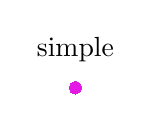
\begin{tikzpicture}

% defining custom colors
\definecolor{mycolor1}{rgb}{1,0.1,0.1}
\definecolor{mycolor2}{rgb}{0.1,1,0.1}
\definecolor{mycolor3}{rgb}{0.1,0.1,1}
\definecolor{mycolor4}{rgb}{0.4,0.4,0.1}
\definecolor{mycolor5}{rgb}{0.1,1,1}
\definecolor{mycolor6}{rgb}{0.9,0.1,0.9}


\begin{axis}[%
view={-72}{42},
xmin=0, xmax=100,
xlabel={Number of samples},
xmajorgrids,
y dir=reverse,
ymin=-4, ymax=4,
ylabel={sample location},
ymajorgrids,
zmin=0, zmax=0.4,
zmajorgrids,
axis lines=left,
scale only axis,
width=\fwidth,
height=\fheight,
title={simple}]
\addplot3 [
color=mycolor1,
only marks,
mark=*,
mark options={solid}
]
coordinates{
 (1,0.864397318249258,0)(2,0.094202610858281,0)(3,-0.851909224508774,0)(4,0.873504449150106,0)(5,-0.438039043088074,0)(6,-0.429661051911298,0)(7,-1.10272856023819,0)(8,0.39624682112797,0)(9,-0.964925101622627,0)(10,0.168448763331274,0)(11,-1.96535886818246,0)(12,-0.744302088643632,0)(13,-0.552306700484431,0)(14,-0.819726048957947,0)(15,1.10914180018547,0)(16,-0.614945861779945,0)(17,-0.254635294228131,0)(18,-0.26982964643979,0)(19,-1.67199406378983,0)(20,-1.87604530491713,0)(21,0.575006015878006,0)(22,-0.866133150431014,0)(23,-2.11652270104548,0)(24,-0.964465668893709,0)(25,0.212729440847614,0)(26,0.477917410863812,0)(27,0.10065773429252,0)(28,0.297433365310199,0)(29,0.570148492190659,0)(30,-1.62449561946395,0)(31,0.643442896614198,0)(32,0.681861101501212,0)(33,0.0146545462976063,0)(34,-1.30154083556885,0)(35,-1.28458694199502,0)(36,0.812213221007246,0)(37,0.838548117504491,0)(38,1.42032099924033,0)(39,-0.989751963936141,0)(40,-1.18322927670026,0)(41,-0.466258701033501,0)(42,-0.365943456601606,0)(43,1.11833282594471,0)(44,-0.465614764979949,0)(45,-1.56079951442098,0)(46,-0.283103049634655,0)(47,-1.32294142478163,0)(48,-0.196238020663121,0)(49,0.419039092209372,0)(50,0.742318242363705,0)(51,-0.143031901660663,0)(52,-2.16194345485188,0)(53,-0.644226188013935,0)(54,1.43958966362552,0)(55,-0.846916703704845,0)(56,0.0573396598842837,0)(57,0.643407819310009,0)(58,-0.670431031039433,0)(59,-0.00314182038723435,0)(60,0.35293137585827,0)(61,1.17950226794027,0)(62,-0.685902078686398,0)(63,1.67678943259546,0)(64,-0.255308776295612,0)(65,-0.647548492231093,0)(66,-0.182214217198884,0)(67,0.851800292262651,0)(68,-0.306550037434344,0)(69,-0.440528888444301,0)(70,-0.611471876975789,0)(71,-0.485206910127117,0)(72,1.19701928905678,0)(73,1.39478769033299,0)(74,0.165367561474691,0)(75,-0.509966956368727,0)(76,1.37771664896642,0)(77,1.29851755410422,0)(78,-0.130117041997769,0)(79,0.740248586252175,0)(80,1.3320174467912,0)(81,-0.278070689182663,0)(82,-0.327992902252155,0)(83,-0.0125272443409905,0)(84,0.903178709204238,0)(85,-1.11246332865596,0)(86,-0.839210796544983,0)(87,0.0355343920326862,0)(88,-1.24652893677206,0)(89,0.884505037335452,0)(90,2.53833384421976,0)(91,1.31679503886664,0)(92,1.44221307180034,0)(93,1.46691939938362,0)(94,-1.10705180813558,0)(95,-0.460936138301192,0)(96,-0.0202959162388906,0)(97,-0.0459981798696434,0)(98,-0.544486576241684,0)(99,0.917034563222667,0)(100,-0.0194183076797647,0) 
};

\addplot3 [
color=mycolor2,
only marks,
mark=*,
mark options={solid}
]
coordinates{
 (1,0.894186799433926,0)(2,0.624789448518379,0)(3,0.901015809078886,0)(4,0.76249570105499,0)(5,0.626624946464636,0)(6,0.277911557337548,0)(7,0.40321580437412,0)(8,0.0980796951144261,0)(9,0.151347871230974,0)(10,-0.470153173075747,0)(11,-0.705522159809189,0)(12,-0.880176873859512,0)(13,-1.13939701106729,0)(14,-0.788655577398747,0)(15,-0.983118533490718,0)(16,-1.06364128373352,0)(17,-1.14896891003229,0)(18,-1.14896891003229,0)(19,-1.74222652575261,0)(20,-1.56039365790527,0)(21,-1.56039365790527,0)(22,-1.56039365790527,0)(23,-1.86538448177946,0)(24,-1.79811352593421,0)(25,-1.64698277075619,0)(26,-1.61515200030855,0)(27,-1.52109531165764,0)(28,-1.34079852767432,0)(29,-1.85450914832154,0)(30,-1.65103463856583,0)(31,-1.43541122570432,0)(32,-1.43077705126664,0)(33,-1.43077705126664,0)(34,-1.43077705126664,0)(35,-1.17393267885818,0)(36,-0.908760480962106,0)(37,-0.459615544345533,0)(38,-0.459615544345533,0)(39,-0.833785495202175,0)(40,-0.981229442615912,0)(41,-0.981229442615912,0)(42,-0.627581551404118,0)(43,-0.774821868358182,0)(44,-0.774821868358182,0)(45,-0.864346913296703,0)(46,-0.864346913296703,0)(47,-0.864346913296703,0)(48,-0.73183511729361,0)(49,-0.49709347783739,0)(50,-0.542324136568681,0)(51,-1.22599068555121,0)(52,-1.22599068555121,0)(53,-0.770752462241984,0)(54,-1.03857103945691,0)(55,-1.02043864690754,0)(56,-0.816975229569369,0)(57,-1.02898413678333,0)(58,-1.02997766762562,0)(59,-0.918370967080706,0)(60,-0.54537959987816,0)(61,-0.762280881927465,0)(62,-0.23203350557716,0)(63,-0.312769229549614,0)(64,-0.517542042635425,0)(65,-0.575163237476735,0)(66,-0.305800333962027,0)(67,-0.402739967472267,0)(68,-0.54204743373089,0)(69,-0.54204743373089,0)(70,-0.695483330976321,0)(71,-0.316952595318832,0)(72,0.124118000062956,0)(73,0.176411814599749,0)(74,0.0151461032448606,0)(75,0.450818361351715,0)(76,0.861445666619741,0)(77,0.820299045108067,0)(78,1.05438620183571,0)(79,1.05438620183571,0)(80,0.966452529000719,0)(81,0.862732066252141,0)(82,0.858770603759842,0)(83,1.14438078928547,0)(84,0.792588996088941,0)(85,0.527207240680309,0)(86,0.538444202089572,0)(87,0.144257141138799,0)(88,0.423962193126028,0)(89,0.423962193126028,0)(90,0.84036934656888,0)(91,1.29643716438458,0)(92,1.29643716438458,0)(93,0.946356644232966,0)(94,0.800595838941552,0)(95,0.794177706690062,0)(96,0.779631805029045,0)(97,0.60745003139798,0)(98,0.897441822686111,0)(99,0.891301214628711,0)(100,1.13626078279853,0) 
};

\addplot3 [
color=mycolor3,
only marks,
mark=*,
mark options={solid}
]
coordinates{
 (1,0.894186799433926,0)(2,0.624789448518379,0)(3,0.901015809078886,0)(4,0.76249570105499,0)(5,0.626624946464636,0)(6,0.277911557337548,0)(7,0.40321580437412,0)(8,0.0980796951144261,0)(9,0.151347871230974,0)(10,-0.470153173075747,0)(11,-0.705522159809189,0)(12,-0.880176873859512,0)(13,-1.13939701106729,0)(14,-0.788655577398747,0)(15,-0.983118533490718,0)(16,-1.06364128373352,0)(17,-1.14896891003229,0)(18,-1.14896891003229,0)(19,-1.74222652575261,0)(20,-1.56039365790527,0)(21,-1.56039365790527,0)(22,-1.56039365790527,0)(23,-1.86538448177946,0)(24,-1.79811352593421,0)(25,-1.64698277075619,0)(26,-1.61515200030855,0)(27,-1.52109531165764,0)(28,-1.34079852767432,0)(29,-1.85450914832154,0)(30,-1.65103463856583,0)(31,-1.43541122570432,0)(32,-1.43077705126664,0)(33,-1.43077705126664,0)(34,-1.43077705126664,0)(35,-1.17393267885818,0)(36,-0.908760480962106,0)(37,-0.459615544345533,0)(38,-0.459615544345533,0)(39,-0.833785495202175,0)(40,-0.981229442615912,0)(41,-0.981229442615912,0)(42,-0.627581551404118,0)(43,-0.774821868358182,0)(44,-0.774821868358182,0)(45,-0.864346913296703,0)(46,-0.864346913296703,0)(47,-0.864346913296703,0)(48,-0.73183511729361,0)(49,-0.49709347783739,0)(50,-0.542324136568681,0)(51,-1.22599068555121,0)(52,-1.22599068555121,0)(53,-0.770752462241984,0)(54,-1.03857103945691,0)(55,-1.02043864690754,0)(56,-0.816975229569369,0)(57,-1.02898413678333,0)(58,-1.02997766762562,0)(59,-0.918370967080706,0)(60,-0.54537959987816,0)(61,-0.762280881927465,0)(62,-0.23203350557716,0)(63,-0.312769229549614,0)(64,-0.517542042635425,0)(65,-0.575163237476735,0)(66,-0.305800333962027,0)(67,-0.402739967472267,0)(68,-0.54204743373089,0)(69,-0.54204743373089,0)(70,-0.695483330976321,0)(71,-0.316952595318832,0)(72,0.124118000062956,0)(73,0.176411814599749,0)(74,0.0151461032448606,0)(75,0.450818361351715,0)(76,0.861445666619741,0)(77,0.820299045108067,0)(78,1.05438620183571,0)(79,1.05438620183571,0)(80,0.966452529000719,0)(81,0.862732066252141,0)(82,0.858770603759842,0)(83,1.14438078928547,0)(84,0.792588996088941,0)(85,0.527207240680309,0)(86,0.538444202089572,0)(87,0.144257141138799,0)(88,0.423962193126028,0)(89,0.423962193126028,0)(90,0.84036934656888,0)(91,1.29643716438458,0)(92,1.29643716438458,0)(93,0.946356644232966,0)(94,0.800595838941552,0)(95,0.794177706690062,0)(96,0.779631805029045,0)(97,0.60745003139798,0)(98,0.897441822686111,0)(99,0.891301214628711,0)(100,1.13626078279853,0) 
};

\addplot3 [
color=mycolor4,
only marks,
mark=*,
mark options={solid}
]
coordinates{
 (1,0,0)(2,-1.33128178779202,0)(3,1.15616106490586,0)(4,-0.819857372188568,0)(5,-0.822315683258383,0)(6,0.0101052362649342,0)(7,0.0100199658716916,0)(8,-2.99124612929279,0)(9,0.746802303049927,0)(10,2.01925804340992,0)(11,0.769541383175744,0)(12,-0.555214351987828,0)(13,0.735803559078723,0)(14,-0.53837469178382,0)(15,0.715012425586035,0)(16,-0.529364928692513,0)(17,-0.527396753166929,0)(18,-1.02296281378926,0)(19,0.690581427317872,0)(20,-0.53686214405986,0)(21,0.694917817134954,0)(22,-0.537302549942372,0)(23,-0.533965804885554,0)(24,0.689080060250669,0)(25,-2.15599746259838,0)(26,-0.105275316545479,0)(27,-0.824561759528231,0)(28,0.47011156182833,0)(29,-0.626666227973692,0)(30,0.477058604626624,0)(31,-0.771635343541967,0)(32,-0.756766973307908,0)(33,0.487424364492131,0)(34,-0.687283067972383,0)(35,1.92402163326157,0)(36,1.93649484481022,0)(37,0.527092955905229,0)(38,0.53943514825233,0)(39,0.566005583787015,0)(40,-0.090855847709705,0)(41,-0.105275316545479,0)(42,-0.824561759528231,0)(43,0.598269744340244,0)(44,-0.626666227973692,0)(45,0.365589555143974,0)(46,-0.771635343541967,0)(47,-0.673706752405501,0)(48,0.634747902398438,0)(49,-0.12274694683746,0)(50,1.95064567700377,0)(51,1.59017527514621,0)(52,0.591368286455537,0)(53,0.339636544799008,0)(54,0.317562026337821,0)(55,-0.090855847709705,0)(56,0.621208799266072,0)(57,0.29466788463721,0)(58,-0.825536409346696,0)(59,-0.567090108836959,0)(60,1.58930706131936,0)(61,-0.830653737839016,0)(62,0.462673513904619,0)(63,-0.586946235913247,0)(64,-0.105275316545479,0)(65,-0.824561759528231,0)(66,0.457917225859266,0)(67,-0.626666227973692,0)(68,0.302722266977014,0)(69,-0.771635343541967,0)(70,-0.586465606341159,0)(71,0.635703963615292,0)(72,-0.12274694683746,0)(73,1.95353986927408,0)(74,1.95301485779942,0)(75,-0.0848456051344682,0)(76,0.348584544735474,0)(77,0.317562026337821,0)(78,-0.090855847709705,0)(79,0.618009059732205,0)(80,0.600989761610443,0)(81,-0.829084480401453,0)(82,-0.461807231299709,0)(83,1.58533262933372,0)(84,-1.31063646161906,0)(85,0.26997478861888,0)(86,-0.553580924410985,0)(87,-0.885244446909254,0)(88,0.253929892316978,0)(89,0.389876870194523,0)(90,1.58437291888327,0)(91,-0.886465268512436,0)(92,1.95302090372003,0)(93,-0.136649296170648,0)(94,0.308762330285705,0)(95,0.189793147403423,0)(96,0.603899653280435,0)(97,1.58402553049076,0)(98,0.610822726249642,0)(99,0.351859513355818,0)(100,0.174218580508368,0) 
};

\addplot3 [
color=mycolor5,
only marks,
mark=*,
mark options={solid}
]
coordinates{
 (1,0.864397318249258,0)(2,0.094202610858281,0)(3,-0.851909224508774,0)(4,0.873504449150106,0)(5,-0.438039043088074,0)(6,-0.429661051911298,0)(7,-1.10272856023819,0)(8,0.39624682112797,0)(9,-0.964925101622627,0)(10,0.168448763331274,0)(11,0,0)(12,-2.99984229028101,0)(13,-0.492834125418496,0)(14,-0.492764178429169,0)(15,-1.01010396312064,0)(16,0.170949658305456,0)(17,-0.492472563225201,0)(18,-0.49242888561874,0)(19,-0.492358310997743,0)(20,-2.99862889165853,0)(21,-2.99840802857503,0)(22,-2.99826516463408,0)(23,-1.01015872251978,0)(24,-2.99815989437713,0)(25,-1.01013695282469,0)(26,0.170989573752006,0)(27,0.170974212566408,0)(28,0.171002647585496,0)(29,0.171029825664793,0)(30,2.9984940356494,0)(31,-2.99805255706076,0)(32,0.83303197814675,0)(33,0.832865625028656,0)(34,0.174078423895961,0)(35,-1.00569327742335,0)(36,-1.00569149030135,0)(37,0.832858052531542,0)(38,0.832818920309209,0)(39,2.82689070696099,0)(40,-1.00135719452385,0)(41,-1.00132405881972,0)(42,-0.489186317823382,0)(43,-0.489219967594414,0)(44,-0.489357796056204,0)(45,-0.489191978640337,0)(46,-2.9946578833904,0)(47,-0.489327887493734,0)(48,-0.489306833210894,0)(49,-0.489299910556622,0)(50,0.183057431585286,0)(51,0.825869621452296,0)(52,-1.00125201912759,0)(53,-2.99432935586456,0)(54,-0.48935723978245,0)(55,2.81599256079584,0)(56,-1.00133619271988,0)(57,0.182870591538854,0)(58,0.825884152905312,0)(59,-0.489202759480156,0)(60,0.182981019868393,0)(61,0.183023888028671,0)(62,0.825894714515985,0)(63,-0.489200500791873,0)(64,2.81483633601357,0)(65,-0.489160522164958,0)(66,-0.489153634789065,0)(67,-0.489151156106985,0)(68,0.82588100917097,0)(69,-0.489136607972968,0)(70,-0.489134713620376,0)(71,-0.489158971466028,0)(72,-0.489219990481902,0)(73,0.825882691249404,0)(74,2.8147685474818,0)(75,0.182781800846237,0)(76,-0.489119943466127,0)(77,0.182782696741198,0)(78,-0.489126425114395,0)(79,0.825878872050626,0)(80,0.825866650445372,0)(81,0.82583719552863,0)(82,-0.489118267972671,0)(83,-0.489247897191441,0)(84,0.182914232264688,0)(85,0.825859768968774,0)(86,-1.00132825844407,0)(87,-1.00136517321485,0)(88,0.182815708436891,0)(89,-1.00135940762781,0)(90,0.825878473194729,0)(91,2.81379300783293,0)(92,-1.00136819242384,0)(93,2.98503476467164,0)(94,2.81654418892335,0)(95,-1.00139511788827,0)(96,-0.489026254191439,0)(97,0.182776917312112,0)(98,0.182654950282649,0)(99,-0.489024631646551,0)(100,0.825924449738613,0) 
};

\addplot3 [
color=mycolor6,
only marks,
mark=*,
mark options={solid}
]
coordinates{
 (1,0.894186799433926,0)(2,0.624789448518379,0)(3,0.901015809078886,0)(4,0.76249570105499,0)(5,0.626624946464636,0)(6,0.277911557337548,0)(7,0.40321580437412,0)(8,0.0980796951144261,0)(9,0.151347871230974,0)(10,-0.470153173075747,0)(11,-0.705522159809189,0)(12,-0.880176873859512,0)(13,-1.13939701106729,0)(14,-0.788655577398747,0)(15,-0.983118533490718,0)(16,-1.06364128373352,0)(17,-1.14896891003229,0)(18,-1.14896891003229,0)(19,-1.74222652575261,0)(20,-1.56039365790527,0)(21,-1.56039365790527,0)(22,-1.56039365790527,0)(23,-1.86538448177946,0)(24,-1.79811352593421,0)(25,-1.64698277075619,0)(26,-1.61515200030855,0)(27,-1.52109531165764,0)(28,-1.34079852767432,0)(29,-1.85450914832154,0)(30,-1.65103463856583,0)(31,-1.43541122570432,0)(32,-1.43077705126664,0)(33,-1.43077705126664,0)(34,-1.43077705126664,0)(35,-1.17393267885818,0)(36,-0.908760480962106,0)(37,-0.459615544345533,0)(38,-0.459615544345533,0)(39,-0.833785495202175,0)(40,-0.981229442615912,0)(41,-0.981229442615912,0)(42,-0.627581551404118,0)(43,-0.774821868358182,0)(44,-0.774821868358182,0)(45,-0.864346913296703,0)(46,-0.864346913296703,0)(47,-0.864346913296703,0)(48,-0.73183511729361,0)(49,-0.49709347783739,0)(50,-0.542324136568681,0)(51,-1.22599068555121,0)(52,-1.22599068555121,0)(53,-0.770752462241984,0)(54,-1.03857103945691,0)(55,-1.02043864690754,0)(56,-0.816975229569369,0)(57,-1.02898413678333,0)(58,-1.02997766762562,0)(59,-0.918370967080706,0)(60,-0.54537959987816,0)(61,-0.762280881927465,0)(62,-0.23203350557716,0)(63,-0.312769229549614,0)(64,-0.517542042635425,0)(65,-0.575163237476735,0)(66,-0.305800333962027,0)(67,-0.402739967472267,0)(68,-0.54204743373089,0)(69,-0.54204743373089,0)(70,-0.695483330976321,0)(71,-0.316952595318832,0)(72,0.124118000062956,0)(73,0.176411814599749,0)(74,0.0151461032448606,0)(75,0.450818361351715,0)(76,0.861445666619741,0)(77,0.820299045108067,0)(78,1.05438620183571,0)(79,1.05438620183571,0)(80,0.966452529000719,0)(81,0.862732066252141,0)(82,0.858770603759842,0)(83,1.14438078928547,0)(84,0.792588996088941,0)(85,0.527207240680309,0)(86,0.538444202089572,0)(87,0.144257141138799,0)(88,0.423962193126028,0)(89,0.423962193126028,0)(90,0.84036934656888,0)(91,1.29643716438458,0)(92,1.29643716438458,0)(93,0.946356644232966,0)(94,0.800595838941552,0)(95,0.794177706690062,0)(96,0.779631805029045,0)(97,0.60745003139798,0)(98,0.897441822686111,0)(99,0.891301214628711,0)(100,1.13626078279853,0) 
};

\addplot3 [
color=black,
solid,
line width=2.0pt
]
coordinates{
 (101,-4,0.000133830225764885)(101,-3.99199199199199,0.000138182046410498)(101,-3.98398398398398,0.000142666228042307)(101,-3.97597597597598,0.000147286481503254)(101,-3.96796796796797,0.000152046611333821)(101,-3.95995995995996,0.000156950517814782)(101,-3.95195195195195,0.00016200219904485)(101,-3.94394394394394,0.00016720575305353)(101,-3.93593593593594,0.000172565379949496)(101,-3.92792792792793,0.00017808538410479)(101,-3.91991991991992,0.000183770176375138)(101,-3.91191191191191,0.000189624276356684)(101,-3.9039039039039,0.000195652314679408)(101,-3.8958958958959,0.000201859035337516)(101,-3.88788788788789,0.000208249298057069)(101,-3.87987987987988,0.000214828080701088)(101,-3.87187187187187,0.000221600481712427)(101,-3.86386386386386,0.0002285717225946)(101,-3.85585585585586,0.000235747150430845)(101,-3.84784784784785,0.000243132240441603)(101,-3.83983983983984,0.000250732598580649)(101,-3.83183183183183,0.00025855396417006)(101,-3.82382382382382,0.000266602212574213)(101,-3.81581581581582,0.000274883357912987)(101,-3.80780780780781,0.000283403555814325)(101,-3.7997997997998,0.000292169106206322)(101,-3.79179179179179,0.000301186456148956)(101,-3.78378378378378,0.0003104622027056)(101,-3.77577577577578,0.000320003095854415)(101,-3.76776776776777,0.000329816041439723)(101,-3.75975975975976,0.000339908104163431)(101,-3.75175175175175,0.00035028651061658)(101,-3.74374374374374,0.000360958652351047)(101,-3.73573573573574,0.000371932088991451)(101,-3.72772772772773,0.000383214551387261)(101,-3.71971971971972,0.000394813944805093)(101,-3.71171171171171,0.000406738352161197)(101,-3.7037037037037,0.000418996037294059)(101,-3.6956956956957,0.00043159544827708)(101,-3.68768768768769,0.00044454522077123)(101,-3.67967967967968,0.000457854181417586)(101,-3.67167167167167,0.000471531351269624)(101,-3.66366366366366,0.000485585949265103)(101,-3.65565565565566,0.000500027395737409)(101,-3.64764764764765,0.000514865315966112)(101,-3.63963963963964,0.000530109543766577)(101,-3.63163163163163,0.000545770125118335)(101,-3.62362362362362,0.000561857321831991)(101,-3.61561561561562,0.00057838161525435)(101,-3.60760760760761,0.000595353710011453)(101,-3.5995995995996,0.000612784537789192)(101,-3.59159159159159,0.000630685261151105)(101,-3.58358358358358,0.000649067277392973)(101,-3.57557557557558,0.000667942222433795)(101,-3.56756756756757,0.000687321974742666)(101,-3.55955955955956,0.000707218659301081)(101,-3.55155155155155,0.000727644651600165)(101,-3.54354354354354,0.000748612581672246)(101,-3.53553553553554,0.000770135338156226)(101,-3.52752752752753,0.000792226072396121)(101,-3.51951951951952,0.000814898202572139)(101,-3.51151151151151,0.000838165417863603)(101,-3.5035035035035,0.000862041682643006)(101,-3.4954954954955,0.000886541240700502)(101,-3.48748748748749,0.00091167861949796)(101,-3.47947947947948,0.000937468634451867)(101,-3.47147147147147,0.000963926393244149)(101,-3.46346346346346,0.00099106730016006)(101,-3.45545545545546,0.0010189070604522)(101,-3.44744744744745,0.00104746168472971)(101,-3.43943943943944,0.0010767474933716)(101,-3.43143143143143,0.00110678112096323)(101,-3.42342342342342,0.00113757952075483)(101,-3.41541541541542,0.00116915996914087)(101,-3.40740740740741,0.00120154007015926)(101,-3.3993993993994,0.00123473776000907)(101,-3.39139139139139,0.00126877131158549)(101,-3.38338338338338,0.00130365933903088)(101,-3.37537537537538,0.00133942080230046)(101,-3.36736736736737,0.00137607501174126)(101,-3.35935935935936,0.00141364163268301)(101,-3.35135135135135,0.00145214069003938)(101,-3.34334334334334,0.0014915925729182)(101,-3.33533533533534,0.00153201803923895)(101,-3.32732732732733,0.00157343822035606)(101,-3.31931931931932,0.00161587462568624)(101,-3.31131131131131,0.00165934914733832)(101,-3.3033033033033,0.00170388406474362)(101,-3.2952952952953,0.00174950204928538)(101,-3.28728728728729,0.00179622616892505)(101,-3.27927927927928,0.00184407989282385)(101,-3.27127127127127,0.00189308709595757)(101,-3.26326326326326,0.00194327206372255)(101,-3.25525525525526,0.00199465949653091)(101,-3.24724724724725,0.00204727451439301)(101,-3.23923923923924,0.00210114266148476)(101,-3.23123123123123,0.00215628991069791)(101,-3.22322322322322,0.00221274266817093)(101,-3.21521521521522,0.00227052777779815)(101,-3.20720720720721,0.00232967252571501)(101,-3.1991991991992,0.00239020464475689)(101,-3.19119119119119,0.00245215231888918)(101,-3.18318318318318,0.00251554418760605)(101,-3.17517517517518,0.00258040935029545)(101,-3.16716716716717,0.00264677737056774)(101,-3.15915915915916,0.00271467828054534)(101,-3.15115115115115,0.00278414258511062)(101,-3.14314314314314,0.00285520126610952)(101,-3.13513513513514,0.00292788578650791)(101,-3.12712712712713,0.00300222809449793)(101,-3.11911911911912,0.00307826062755151)(101,-3.11111111111111,0.00315601631641805)(101,-3.1031031031031,0.00323552858906328)(101,-3.0950950950951,0.00331683137454643)(101,-3.08708708708709,0.00339995910683238)(101,-3.07907907907908,0.00348494672853595)(101,-3.07107107107107,0.00357182969459489)(101,-3.06306306306306,0.00366064397586864)(101,-3.05505505505506,0.00375142606265932)(101,-3.04704704704705,0.00384421296815189)(101,-3.03903903903904,0.00393904223176991)(101,-3.03103103103103,0.00403595192244368)(101,-3.02302302302302,0.0041349806417872)(101,-3.01501501501502,0.00423616752718052)(101,-3.00700700700701,0.00433955225475399)(101,-2.998998998999,0.00444517504227067)(101,-2.99099099099099,0.00455307665190355)(101,-2.98298298298298,0.00466329839290368)(101,-2.97497497497497,0.00477588212415564)(101,-2.96696696696697,0.00489087025661667)(101,-2.95895895895896,0.00500830575563558)(101,-2.95095095095095,0.00512823214314764)(101,-2.94294294294294,0.00525069349974171)(101,-2.93493493493493,0.00537573446659573)(101,-2.92692692692693,0.00550340024727644)(101,-2.91891891891892,0.00563373660939975)(101,-2.91091091091091,0.0057667898861475)(101,-2.9029029029029,0.00590260697763674)(101,-2.89489489489489,0.00604123535213747)(101,-2.88688688688689,0.00618272304713484)(101,-2.87887887887888,0.00632711867023163)(101,-2.87087087087087,0.00647447139988703)(101,-2.86286286286286,0.00662483098598741)(101,-2.85485485485485,0.0067782477502453)(101,-2.84684684684685,0.00693477258642191)(101,-2.83883883883884,0.00709445696036946)(101,-2.83083083083083,0.00725735290988894)(101,-2.82282282282282,0.00742351304439893)(101,-2.81481481481481,0.00759299054441176)(101,-2.80680680680681,0.00776583916081211)(101,-2.7987987987988,0.00794211321393437)(101,-2.79079079079079,0.00812186759243432)(101,-2.78278278278278,0.00830515775195071)(101,-2.77477477477477,0.00849203971355293)(101,-2.76676676676677,0.00868257006197001)(101,-2.75875875875876,0.00887680594359712)(101,-2.75075075075075,0.00907480506427511)(101,-2.74274274274274,0.00927662568683898)(101,-2.73473473473473,0.00948232662843099)(101,-2.72672672672673,0.00969196725757422)(101,-2.71871871871872,0.00990560749100246)(101,-2.71071071071071,0.0101233077902421)(101,-2.7027027027027,0.0103451291579421)(101,-2.69469469469469,0.0105711331339476)(101,-2.68668668668669,0.0108013817911136)(101,-2.67867867867868,0.011035937730854)(101,-2.67067067067067,0.0112748640784219)(101,-2.66266266266266,0.0115182244779185)(101,-2.65465465465465,0.0117660830870247)(101,-2.64664664664665,0.0120185045714526)(101,-2.63863863863864,0.0122755540991133)(101,-2.63063063063063,0.0125372973339956)(101,-2.62262262262262,0.0128038004297541)(101,-2.61461461461461,0.0130751300230007)(101,-2.60660660660661,0.0133513532262973)(101,-2.5985985985986,0.0136325376208454)(101,-2.59059059059059,0.0139187512488692)(101,-2.58258258258258,0.014210062605689)(101,-2.57457457457457,0.0145065406314803)(101,-2.56656656656657,0.0148082547027168)(101,-2.55855855855856,0.0151152746232934)(101,-2.55055055055055,0.0154276706153247)(101,-2.54254254254254,0.0157455133096184)(101,-2.53453453453453,0.0160688737358178)(101,-2.52652652652653,0.016397823312213)(101,-2.51851851851852,0.0167324338352151)(101,-2.51051051051051,0.0170727774684938)(101,-2.5025025025025,0.0174189267317727)(101,-2.49449449449449,0.0177709544892815)(101,-2.48648648648649,0.0181289339378627)(101,-2.47847847847848,0.0184929385947284)(101,-2.47047047047047,0.0188630422848682)(101,-2.46246246246246,0.0192393191281025)(101,-2.45445445445445,0.0196218435257817)(101,-2.44644644644645,0.0200106901471285)(101,-2.43843843843844,0.020405933915221)(101,-2.43043043043043,0.0208076499926159)(101,-2.42242242242242,0.0212159137666093)(101,-2.41441441441441,0.0216308008341344)(101,-2.40640640640641,0.0220523869862944)(101,-2.3983983983984,0.0224807481925294)(101,-2.39039039039039,0.022915960584417)(101,-2.38238238238238,0.0233581004391047)(101,-2.37437437437437,0.023807244162374)(101,-2.36636636636637,0.0242634682713357)(101,-2.35835835835836,0.0247268493767558)(101,-2.35035035035035,0.0251974641650118)(101,-2.34234234234234,0.0256753893796796)(101,-2.33433433433433,0.0261607018027501)(101,-2.32632632632633,0.0266534782354775)(101,-2.31831831831832,0.0271537954788581)(101,-2.31031031031031,0.0276617303137407)(101,-2.3023023023023,0.0281773594805703)(101,-2.29429429429429,0.0287007596587648)(101,-2.28628628628629,0.0292320074457259)(101,-2.27827827827828,0.029771179335487)(101,-2.27027027027027,0.0303183516969979)(101,-2.26226226226226,0.0308736007520491)(101,-2.25425425425425,0.0314370025528369)(101,-2.24624624624625,0.0320086329591723)(101,-2.23823823823824,0.0325885676153351)(101,-2.23023023023023,0.0331768819265761)(101,-2.22222222222222,0.0337736510352706)(101,-2.21421421421421,0.0343789497967251)(101,-2.20620620620621,0.0349928527546413)(101,-2.1981981981982,0.0356154341162401)(101,-2.19019019019019,0.0362467677270497)(101,-2.18218218218218,0.0368869270453615)(101,-2.17417417417417,0.0375359851163567)(101,-2.16616616616617,0.03819401454591)(101,-2.15815815815816,0.0388610874740724)(101,-2.15015015015015,0.03953727554824)(101,-2.14214214214214,0.0402226498960119)(101,-2.13413413413413,0.0409172810977437)(101,-2.12612612612613,0.0416212391588003)(101,-2.11811811811812,0.0423345934815158)(101,-2.11011011011011,0.0430574128368641)(101,-2.1021021021021,0.043789765335848)(101,-2.09409409409409,0.0445317184006116)(101,-2.08608608608609,0.0452833387352837)(101,-2.07807807807808,0.0460446922965577)(101,-2.07007007007007,0.0468158442640166)(101,-2.06206206206206,0.047596859010209)(101,-2.05405405405405,0.0483878000704834)(101,-2.04604604604605,0.0491887301125894)(101,-2.03803803803804,0.0499997109060533)(101,-2.03003003003003,0.0508208032913361)(101,-2.02202202202202,0.0516520671487823)(101,-2.01401401401401,0.0524935613673682)(101,-2.00600600600601,0.053345343813258)(101,-1.997997997998,0.0542074712981785)(101,-1.98998998998999,0.0550799995476186)(101,-1.98198198198198,0.0559629831688667)(101,-1.97397397397397,0.0568564756188931)(101,-1.96596596596597,0.0577605291720876)(101,-1.95795795795796,0.0586751948878651)(101,-1.94994994994995,0.0596005225781457)(101,-1.94194194194194,0.0605365607747232)(101,-1.93393393393393,0.0614833566965309)(101,-1.92592592592593,0.062440956216817)(101,-1.91791791791792,0.06340940383024)(101,-1.90990990990991,0.0643887426198963)(101,-1.9019019019019,0.0653790142242912)(101,-1.89389389389389,0.0663802588042656)(101,-1.88588588588589,0.0673925150098903)(101,-1.87787787787788,0.0684158199473405)(101,-1.86986986986987,0.0694502091457625)(101,-1.86186186186186,0.0704957165241466)(101,-1.85385385385385,0.0715523743582164)(101,-1.84584584584585,0.0726202132473521)(101,-1.83783783783784,0.0736992620815557)(101,-1.82982982982983,0.0747895480084762)(101,-1.82182182182182,0.0758910964005057)(101,-1.81381381381381,0.0770039308219614)(101,-1.80580580580581,0.0781280729963669)(101,-1.7977977977978,0.0792635427738473)(101,-1.78978978978979,0.0804103580986525)(101,-1.78178178178178,0.0815685349768227)(101,-1.77377377377377,0.0827380874440109)(101,-1.76576576576577,0.0839190275334777)(101,-1.75775775775776,0.0851113652442723)(101,-1.74974974974975,0.086315108509615)(101,-1.74174174174174,0.0875302631654975)(101,-1.73373373373373,0.0887568329195139)(101,-1.72572572572573,0.0899948193199404)(101,-1.71771771771772,0.0912442217250772)(101,-1.70970970970971,0.0925050372728685)(101,-1.7017017017017,0.0937772608508177)(101,-1.69369369369369,0.0950608850662112)(101,-1.68568568568569,0.0963559002166691)(101,-1.67767767767768,0.0976622942610364)(101,-1.66966966966967,0.0989800527906321)(101,-1.66166166166166,0.100309159000872)(101,-1.65365365365365,0.10164959366328)(101,-1.64564564564565,0.103001335097907)(101,-1.63763763763764,0.10436435914617)(101,-1.62962962962963,0.105738639144131)(101,-1.62162162162162,0.107124145896225)(101,-1.61361361361361,0.108520847649465)(101,-1.60560560560561,0.10992871006813)(101,-1.5975975975976,0.111347696208955)(101,-1.58958958958959,0.112777766496842)(101,-1.58158158158158,0.114218878701105)(101,-1.57357357357357,0.115670987912262)(101,-1.56556556556557,0.117134046519405)(101,-1.55755755755756,0.11860800418814)(101,-1.54954954954955,0.120092807839133)(101,-1.54154154154154,0.121588401627275)(101,-1.53353353353353,0.123094726921466)(101,-1.52552552552553,0.124611722285057)(101,-1.51751751751752,0.12613932345695)(101,-1.50950950950951,0.127677463333369)(101,-1.5015015015015,0.129226071950339)(101,-1.49349349349349,0.130785076466857)(101,-1.48548548548549,0.132354401148798)(101,-1.47747747747748,0.133933967353555)(101,-1.46946946946947,0.13552369351543)(101,-1.46146146146146,0.137123495131801)(101,-1.45345345345345,0.13873328475006)(101,-1.44544544544545,0.140352971955359)(101,-1.43743743743744,0.141982463359159)(101,-1.42942942942943,0.143621662588612)(101,-1.42142142142142,0.14527047027677)(101,-1.41341341341341,0.146928784053658)(101,-1.40540540540541,0.148596498538208)(101,-1.3973973973974,0.150273505331067)(101,-1.38938938938939,0.151959693008306)(101,-1.38138138138138,0.153654947116025)(101,-1.37337337337337,0.155359150165875)(101,-1.36536536536537,0.157072181631514)(101,-1.35735735735736,0.158793917945997)(101,-1.34934934934935,0.160524232500122)(101,-1.34134134134134,0.16226299564173)(101,-1.33333333333333,0.164010074675994)(101,-1.32532532532533,0.165765333866673)(101,-1.31731731731732,0.167528634438376)(101,-1.30930930930931,0.169299834579821)(101,-1.3013013013013,0.17107878944811)(101,-1.29329329329329,0.172865351174024)(101,-1.28528528528529,0.174659368868355)(101,-1.27727727727728,0.176460688629273)(101,-1.26926926926927,0.178269153550739)(101,-1.26126126126126,0.18008460373198)(101,-1.25325325325325,0.181906876288021)(101,-1.24524524524525,0.183735805361283)(101,-1.23723723723724,0.185571222134271)(101,-1.22922922922923,0.187412954843324)(101,-1.22122122122122,0.18926082879347)(101,-1.21321321321321,0.191114666374361)(101,-1.20520520520521,0.192974287077311)(101,-1.1971971971972,0.194839507513435)(101,-1.18918918918919,0.19671014143289)(101,-1.18118118118118,0.198585999745227)(101,-1.17317317317317,0.200466890540856)(101,-1.16516516516517,0.202352619113618)(101,-1.15715715715716,0.204242987984477)(101,-1.14914914914915,0.206137796926331)(101,-1.14114114114114,0.208036842989938)(101,-1.13313313313313,0.209939920530956)(101,-1.12512512512513,0.21184682123811)(101,-1.11711711711712,0.21375733416247)(101,-1.10910910910911,0.215671245747847)(101,-1.1011011011011,0.217588339862305)(101,-1.09309309309309,0.219508397830784)(101,-1.08508508508509,0.221431198468836)(101,-1.07707707707708,0.223356518117463)(101,-1.06906906906907,0.225284130679063)(101,-1.06106106106106,0.22721380765447)(101,-1.05305305305305,0.229145318181096)(101,-1.04504504504505,0.231078429072154)(101,-1.03703703703704,0.233012904856966)(101,-1.02902902902903,0.234948507822352)(101,-1.02102102102102,0.236884998055083)(101,-1.01301301301301,0.238822133485401)(101,-1.00500500500501,0.24075966993159)(101,-0.996996996996997,0.242697361145593)(101,-0.988988988988989,0.244634958859672)(101,-0.980980980980981,0.246572212834085)(101,-0.972972972972973,0.248508870905785)(101,-0.964964964964965,0.25044467903813)(101,-0.956956956956957,0.252379381371581)(101,-0.948948948948949,0.254312720275385)(101,-0.940940940940941,0.256244436400228)(101,-0.932932932932933,0.258174268731856)(101,-0.924924924924925,0.260101954645624)(101,-0.916916916916917,0.262027229961987)(101,-0.908908908908909,0.263949829002911)(101,-0.900900900900901,0.265869484649171)(101,-0.892892892892893,0.267785928398552)(101,-0.884884884884885,0.269698890424904)(101,-0.876876876876877,0.271608099638066)(101,-0.868868868868869,0.273513283744617)(101,-0.860860860860861,0.275414169309444)(101,-0.852852852852853,0.277310481818125)(101,-0.844844844844845,0.279201945740075)(101,-0.836836836836837,0.281088284592474)(101,-0.828828828828829,0.282969221004931)(101,-0.820820820820821,0.284844476784867)(101,-0.812812812812813,0.286713772983616)(101,-0.804804804804805,0.288576829963198)(101,-0.796796796796797,0.290433367463758)(101,-0.788788788788789,0.292283104671645)(101,-0.780780780780781,0.294125760288111)(101,-0.772772772772773,0.295961052598604)(101,-0.764764764764765,0.29778869954263)(101,-0.756756756756757,0.299608418784177)(101,-0.748748748748749,0.301419927782648)(101,-0.740740740740741,0.303222943864308)(101,-0.732732732732733,0.305017184294205)(101,-0.724724724724725,0.306802366348536)(101,-0.716716716716717,0.308578207387456)(101,-0.708708708708709,0.310344424928268)(101,-0.700700700700701,0.312100736719007)(101,-0.692692692692693,0.313846860812361)(101,-0.684684684684685,0.31558251563992)(101,-0.676676676676677,0.317307420086723)(101,-0.668668668668669,0.319021293566066)(101,-0.660660660660661,0.320723856094559)(101,-0.652652652652653,0.322414828367396)(101,-0.644644644644645,0.324093931833804)(101,-0.636636636636636,0.325760888772662)(101,-0.628628628628629,0.327415422368237)(101,-0.62062062062062,0.329057256786028)(101,-0.612612612612613,0.330686117248681)(101,-0.604604604604605,0.33230173011195)(101,-0.596596596596596,0.333903822940662)(101,-0.588588588588589,0.335492124584683)(101,-0.58058058058058,0.337066365254824)(101,-0.572572572572573,0.338626276598684)(101,-0.564564564564565,0.340171591776383)(101,-0.556556556556556,0.341702045536168)(101,-0.548548548548549,0.343217374289848)(101,-0.54054054054054,0.344717316188045)(101,-0.532532532532533,0.346201611195215)(101,-0.524524524524525,0.347670001164422)(101,-0.516516516516516,0.349122229911825)(101,-0.508508508508509,0.350558043290856)(101,-0.5005005005005,0.351977189266054)(101,-0.492492492492492,0.353379417986526)(101,-0.484484484484485,0.354764481859011)(101,-0.476476476476476,0.356132135620502)(101,-0.468468468468469,0.357482136410418)(101,-0.46046046046046,0.358814243842273)(101,-0.452452452452452,0.36012822007484)(101,-0.444444444444445,0.361423829882744)(101,-0.436436436436436,0.362700840726495)(101,-0.428428428428429,0.363959022821904)(101,-0.42042042042042,0.365198149208855)(101,-0.412412412412412,0.366417995819425)(101,-0.404404404404405,0.3676183415453)(101,-0.396396396396396,0.368798968304465)(101,-0.388388388388389,0.369959661107154)(101,-0.38038038038038,0.37110020812101)(101,-0.372372372372372,0.372220400735444)(101,-0.364364364364364,0.373320033625156)(101,-0.356356356356356,0.374398904812801)(101,-0.348348348348348,0.375456815730761)(101,-0.34034034034034,0.376493571282005)(101,-0.332332332332332,0.377508979900006)(101,-0.324324324324324,0.378502853607702)(101,-0.316316316316316,0.379475008075448)(101,-0.308308308308308,0.380425262677969)(101,-0.3003003003003,0.38135344055026)(101,-0.292292292292292,0.382259368642425)(101,-0.284284284284284,0.38314287777343)(101,-0.276276276276276,0.384003802683735)(101,-0.268268268268268,0.3848419820868)(101,-0.26026026026026,0.385657258719425)(101,-0.252252252252252,0.386449479390916)(101,-0.244244244244244,0.387218495031049)(101,-0.236236236236236,0.387964160736805)(101,-0.228228228228228,0.38868633581787)(101,-0.22022022022022,0.389384883840873)(101,-0.212212212212212,0.390059672672329)(101,-0.204204204204204,0.390710574520297)(101,-0.196196196196196,0.391337465974705)(101,-0.188188188188188,0.39194022804635)(101,-0.18018018018018,0.392518746204527)(101,-0.172172172172172,0.393072910413305)(101,-0.164164164164164,0.393602615166401)(101,-0.156156156156156,0.394107759520658)(101,-0.148148148148148,0.394588247128102)(101,-0.14014014014014,0.395043986266573)(101,-0.132132132132132,0.3954748898689)(101,-0.124124124124124,0.395880875550626)(101,-0.116116116116116,0.396261865636259)(101,-0.108108108108108,0.396617787184037)(101,-0.1001001001001,0.396948572009207)(101,-0.0920920920920922,0.397254156705792)(101,-0.084084084084084,0.397534482666846)(101,-0.0760760760760761,0.39778949610319)(101,-0.0680680680680679,0.39801914806061)(101,-0.06006006006006,0.398223394435522)(101,-0.0520520520520522,0.398402195989086)(101,-0.0440440440440439,0.398555518359772)(101,-0.0360360360360361,0.398683332074364)(101,-0.0280280280280278,0.398785612557403)(101,-0.02002002002002,0.398862340139061)(101,-0.0120120120120122,0.398913500061449)(101,-0.00400400400400391,0.398939082483343)(101,0.00400400400400436,0.398939082483343)(101,0.0120120120120122,0.398913500061449)(101,0.02002002002002,0.398862340139061)(101,0.0280280280280278,0.398785612557403)(101,0.0360360360360357,0.398683332074364)(101,0.0440440440440444,0.398555518359772)(101,0.0520520520520522,0.398402195989086)(101,0.06006006006006,0.398223394435522)(101,0.0680680680680679,0.39801914806061)(101,0.0760760760760757,0.39778949610319)(101,0.0840840840840844,0.397534482666846)(101,0.0920920920920922,0.397254156705792)(101,0.1001001001001,0.396948572009207)(101,0.108108108108108,0.396617787184037)(101,0.116116116116116,0.396261865636259)(101,0.124124124124124,0.395880875550626)(101,0.132132132132132,0.3954748898689)(101,0.14014014014014,0.395043986266573)(101,0.148148148148148,0.394588247128102)(101,0.156156156156156,0.394107759520658)(101,0.164164164164164,0.393602615166401)(101,0.172172172172172,0.393072910413305)(101,0.18018018018018,0.392518746204527)(101,0.188188188188188,0.39194022804635)(101,0.196196196196196,0.391337465974706)(101,0.204204204204204,0.390710574520297)(101,0.212212212212212,0.390059672672329)(101,0.22022022022022,0.389384883840873)(101,0.228228228228228,0.388686335817871)(101,0.236236236236236,0.387964160736805)(101,0.244244244244245,0.387218495031049)(101,0.252252252252252,0.386449479390916)(101,0.26026026026026,0.385657258719425)(101,0.268268268268268,0.3848419820868)(101,0.276276276276277,0.384003802683735)(101,0.284284284284285,0.38314287777343)(101,0.292292292292292,0.382259368642425)(101,0.3003003003003,0.38135344055026)(101,0.308308308308308,0.380425262677969)(101,0.316316316316317,0.379475008075448)(101,0.324324324324325,0.378502853607702)(101,0.332332332332332,0.377508979900006)(101,0.34034034034034,0.376493571282005)(101,0.348348348348348,0.375456815730761)(101,0.356356356356357,0.374398904812801)(101,0.364364364364365,0.373320033625156)(101,0.372372372372372,0.372220400735444)(101,0.38038038038038,0.37110020812101)(101,0.388388388388388,0.369959661107154)(101,0.396396396396397,0.368798968304465)(101,0.404404404404405,0.3676183415453)(101,0.412412412412412,0.366417995819425)(101,0.42042042042042,0.365198149208855)(101,0.428428428428428,0.363959022821904)(101,0.436436436436437,0.362700840726495)(101,0.444444444444445,0.361423829882744)(101,0.452452452452452,0.36012822007484)(101,0.46046046046046,0.358814243842273)(101,0.468468468468468,0.357482136410418)(101,0.476476476476477,0.356132135620502)(101,0.484484484484485,0.354764481859011)(101,0.492492492492492,0.353379417986526)(101,0.5005005005005,0.351977189266054)(101,0.508508508508508,0.350558043290856)(101,0.516516516516517,0.349122229911825)(101,0.524524524524525,0.347670001164422)(101,0.532532532532533,0.346201611195215)(101,0.54054054054054,0.344717316188045)(101,0.548548548548548,0.343217374289848)(101,0.556556556556557,0.341702045536168)(101,0.564564564564565,0.340171591776383)(101,0.572572572572573,0.338626276598684)(101,0.58058058058058,0.337066365254824)(101,0.588588588588588,0.335492124584683)(101,0.596596596596597,0.333903822940662)(101,0.604604604604605,0.33230173011195)(101,0.612612612612613,0.330686117248681)(101,0.62062062062062,0.329057256786028)(101,0.628628628628628,0.327415422368237)(101,0.636636636636637,0.325760888772662)(101,0.644644644644645,0.324093931833804)(101,0.652652652652653,0.322414828367396)(101,0.66066066066066,0.32072385609456)(101,0.668668668668668,0.319021293566066)(101,0.676676676676677,0.317307420086723)(101,0.684684684684685,0.31558251563992)(101,0.692692692692693,0.313846860812361)(101,0.7007007007007,0.312100736719007)(101,0.708708708708708,0.310344424928268)(101,0.716716716716717,0.308578207387456)(101,0.724724724724725,0.306802366348536)(101,0.732732732732733,0.305017184294205)(101,0.74074074074074,0.303222943864308)(101,0.748748748748748,0.301419927782648)(101,0.756756756756757,0.299608418784177)(101,0.764764764764765,0.29778869954263)(101,0.772772772772773,0.295961052598604)(101,0.780780780780781,0.294125760288111)(101,0.788788788788789,0.292283104671645)(101,0.796796796796797,0.290433367463758)(101,0.804804804804805,0.288576829963198)(101,0.812812812812813,0.286713772983616)(101,0.820820820820821,0.284844476784867)(101,0.828828828828829,0.28296922100493)(101,0.836836836836837,0.281088284592474)(101,0.844844844844845,0.279201945740075)(101,0.852852852852853,0.277310481818125)(101,0.860860860860861,0.275414169309444)(101,0.868868868868869,0.273513283744616)(101,0.876876876876877,0.271608099638066)(101,0.884884884884885,0.269698890424904)(101,0.892892892892893,0.267785928398552)(101,0.900900900900901,0.265869484649172)(101,0.908908908908909,0.263949829002911)(101,0.916916916916917,0.262027229961987)(101,0.924924924924925,0.260101954645624)(101,0.932932932932933,0.258174268731856)(101,0.940940940940941,0.256244436400228)(101,0.948948948948949,0.254312720275384)(101,0.956956956956957,0.252379381371581)(101,0.964964964964965,0.25044467903813)(101,0.972972972972973,0.248508870905785)(101,0.980980980980981,0.246572212834085)(101,0.988988988988989,0.244634958859672)(101,0.996996996996997,0.242697361145593)(101,1.00500500500501,0.24075966993159)(101,1.01301301301301,0.238822133485401)(101,1.02102102102102,0.236884998055083)(101,1.02902902902903,0.234948507822352)(101,1.03703703703704,0.233012904856966)(101,1.04504504504505,0.231078429072154)(101,1.05305305305305,0.229145318181096)(101,1.06106106106106,0.22721380765447)(101,1.06906906906907,0.225284130679062)(101,1.07707707707708,0.223356518117463)(101,1.08508508508509,0.221431198468836)(101,1.09309309309309,0.219508397830784)(101,1.1011011011011,0.217588339862305)(101,1.10910910910911,0.215671245747847)(101,1.11711711711712,0.21375733416247)(101,1.12512512512513,0.21184682123811)(101,1.13313313313313,0.209939920530956)(101,1.14114114114114,0.208036842989938)(101,1.14914914914915,0.206137796926331)(101,1.15715715715716,0.204242987984477)(101,1.16516516516517,0.202352619113618)(101,1.17317317317317,0.200466890540856)(101,1.18118118118118,0.198585999745227)(101,1.18918918918919,0.19671014143289)(101,1.1971971971972,0.194839507513435)(101,1.20520520520521,0.192974287077311)(101,1.21321321321321,0.191114666374361)(101,1.22122122122122,0.18926082879347)(101,1.22922922922923,0.187412954843324)(101,1.23723723723724,0.185571222134271)(101,1.24524524524525,0.183735805361283)(101,1.25325325325325,0.181906876288021)(101,1.26126126126126,0.18008460373198)(101,1.26926926926927,0.178269153550739)(101,1.27727727727728,0.176460688629273)(101,1.28528528528529,0.174659368868355)(101,1.29329329329329,0.172865351174024)(101,1.3013013013013,0.17107878944811)(101,1.30930930930931,0.169299834579821)(101,1.31731731731732,0.167528634438376)(101,1.32532532532533,0.165765333866673)(101,1.33333333333333,0.164010074675994)(101,1.34134134134134,0.16226299564173)(101,1.34934934934935,0.160524232500121)(101,1.35735735735736,0.158793917945997)(101,1.36536536536537,0.157072181631514)(101,1.37337337337337,0.155359150165875)(101,1.38138138138138,0.153654947116025)(101,1.38938938938939,0.151959693008306)(101,1.3973973973974,0.150273505331067)(101,1.40540540540541,0.148596498538208)(101,1.41341341341341,0.146928784053658)(101,1.42142142142142,0.14527047027677)(101,1.42942942942943,0.143621662588612)(101,1.43743743743744,0.141982463359159)(101,1.44544544544545,0.140352971955359)(101,1.45345345345345,0.13873328475006)(101,1.46146146146146,0.137123495131801)(101,1.46946946946947,0.13552369351543)(101,1.47747747747748,0.133933967353555)(101,1.48548548548549,0.132354401148798)(101,1.49349349349349,0.130785076466857)(101,1.5015015015015,0.129226071950339)(101,1.50950950950951,0.127677463333369)(101,1.51751751751752,0.12613932345695)(101,1.52552552552553,0.124611722285057)(101,1.53353353353353,0.123094726921466)(101,1.54154154154154,0.121588401627275)(101,1.54954954954955,0.120092807839133)(101,1.55755755755756,0.11860800418814)(101,1.56556556556557,0.117134046519405)(101,1.57357357357357,0.115670987912262)(101,1.58158158158158,0.114218878701105)(101,1.58958958958959,0.112777766496842)(101,1.5975975975976,0.111347696208955)(101,1.60560560560561,0.10992871006813)(101,1.61361361361361,0.108520847649465)(101,1.62162162162162,0.107124145896225)(101,1.62962962962963,0.105738639144131)(101,1.63763763763764,0.10436435914617)(101,1.64564564564565,0.103001335097907)(101,1.65365365365365,0.10164959366328)(101,1.66166166166166,0.100309159000872)(101,1.66966966966967,0.0989800527906321)(101,1.67767767767768,0.0976622942610364)(101,1.68568568568569,0.0963559002166692)(101,1.69369369369369,0.0950608850662112)(101,1.7017017017017,0.0937772608508176)(101,1.70970970970971,0.0925050372728685)(101,1.71771771771772,0.0912442217250772)(101,1.72572572572573,0.0899948193199405)(101,1.73373373373373,0.088756832919514)(101,1.74174174174174,0.0875302631654974)(101,1.74974974974975,0.086315108509615)(101,1.75775775775776,0.0851113652442723)(101,1.76576576576577,0.0839190275334777)(101,1.77377377377377,0.0827380874440108)(101,1.78178178178178,0.0815685349768226)(101,1.78978978978979,0.0804103580986525)(101,1.7977977977978,0.0792635427738473)(101,1.80580580580581,0.078128072996367)(101,1.81381381381381,0.0770039308219613)(101,1.82182182182182,0.0758910964005057)(101,1.82982982982983,0.0747895480084762)(101,1.83783783783784,0.0736992620815557)(101,1.84584584584585,0.0726202132473521)(101,1.85385385385385,0.0715523743582164)(101,1.86186186186186,0.0704957165241465)(101,1.86986986986987,0.0694502091457625)(101,1.87787787787788,0.0684158199473405)(101,1.88588588588589,0.0673925150098903)(101,1.89389389389389,0.0663802588042655)(101,1.9019019019019,0.0653790142242912)(101,1.90990990990991,0.0643887426198963)(101,1.91791791791792,0.06340940383024)(101,1.92592592592593,0.0624409562168171)(101,1.93393393393393,0.0614833566965309)(101,1.94194194194194,0.0605365607747232)(101,1.94994994994995,0.0596005225781457)(101,1.95795795795796,0.0586751948878651)(101,1.96596596596597,0.0577605291720876)(101,1.97397397397397,0.056856475618893)(101,1.98198198198198,0.0559629831688667)(101,1.98998998998999,0.0550799995476186)(101,1.997997997998,0.0542074712981785)(101,2.00600600600601,0.0533453438132581)(101,2.01401401401401,0.0524935613673681)(101,2.02202202202202,0.0516520671487823)(101,2.03003003003003,0.0508208032913361)(101,2.03803803803804,0.0499997109060533)(101,2.04604604604605,0.0491887301125894)(101,2.05405405405405,0.0483878000704834)(101,2.06206206206206,0.047596859010209)(101,2.07007007007007,0.0468158442640166)(101,2.07807807807808,0.0460446922965577)(101,2.08608608608609,0.0452833387352837)(101,2.09409409409409,0.0445317184006116)(101,2.1021021021021,0.043789765335848)(101,2.11011011011011,0.0430574128368641)(101,2.11811811811812,0.0423345934815158)(101,2.12612612612613,0.0416212391588004)(101,2.13413413413413,0.0409172810977437)(101,2.14214214214214,0.0402226498960119)(101,2.15015015015015,0.03953727554824)(101,2.15815815815816,0.0388610874740724)(101,2.16616616616617,0.03819401454591)(101,2.17417417417417,0.0375359851163567)(101,2.18218218218218,0.0368869270453615)(101,2.19019019019019,0.0362467677270497)(101,2.1981981981982,0.0356154341162401)(101,2.20620620620621,0.0349928527546413)(101,2.21421421421421,0.0343789497967251)(101,2.22222222222222,0.0337736510352706)(101,2.23023023023023,0.0331768819265761)(101,2.23823823823824,0.0325885676153351)(101,2.24624624624625,0.0320086329591724)(101,2.25425425425425,0.0314370025528369)(101,2.26226226226226,0.0308736007520491)(101,2.27027027027027,0.0303183516969979)(101,2.27827827827828,0.029771179335487)(101,2.28628628628629,0.0292320074457258)(101,2.29429429429429,0.0287007596587648)(101,2.3023023023023,0.0281773594805703)(101,2.31031031031031,0.0276617303137407)(101,2.31831831831832,0.0271537954788581)(101,2.32632632632633,0.0266534782354775)(101,2.33433433433433,0.0261607018027501)(101,2.34234234234234,0.0256753893796796)(101,2.35035035035035,0.0251974641650118)(101,2.35835835835836,0.0247268493767558)(101,2.36636636636637,0.0242634682713356)(101,2.37437437437437,0.023807244162374)(101,2.38238238238238,0.0233581004391047)(101,2.39039039039039,0.022915960584417)(101,2.3983983983984,0.0224807481925294)(101,2.40640640640641,0.0220523869862943)(101,2.41441441441441,0.0216308008341344)(101,2.42242242242242,0.0212159137666093)(101,2.43043043043043,0.0208076499926159)(101,2.43843843843844,0.020405933915221)(101,2.44644644644645,0.0200106901471285)(101,2.45445445445445,0.0196218435257817)(101,2.46246246246246,0.0192393191281025)(101,2.47047047047047,0.0188630422848682)(101,2.47847847847848,0.0184929385947284)(101,2.48648648648649,0.0181289339378626)(101,2.49449449449449,0.0177709544892815)(101,2.5025025025025,0.0174189267317727)(101,2.51051051051051,0.0170727774684938)(101,2.51851851851852,0.0167324338352152)(101,2.52652652652653,0.016397823312213)(101,2.53453453453453,0.0160688737358178)(101,2.54254254254254,0.0157455133096184)(101,2.55055055055055,0.0154276706153247)(101,2.55855855855856,0.0151152746232934)(101,2.56656656656657,0.0148082547027168)(101,2.57457457457457,0.0145065406314803)(101,2.58258258258258,0.014210062605689)(101,2.59059059059059,0.0139187512488692)(101,2.5985985985986,0.0136325376208454)(101,2.60660660660661,0.0133513532262973)(101,2.61461461461461,0.0130751300230007)(101,2.62262262262262,0.0128038004297541)(101,2.63063063063063,0.0125372973339956)(101,2.63863863863864,0.0122755540991133)(101,2.64664664664665,0.0120185045714526)(101,2.65465465465465,0.0117660830870247)(101,2.66266266266266,0.0115182244779185)(101,2.67067067067067,0.0112748640784219)(101,2.67867867867868,0.011035937730854)(101,2.68668668668669,0.0108013817911136)(101,2.69469469469469,0.0105711331339476)(101,2.7027027027027,0.0103451291579421)(101,2.71071071071071,0.0101233077902421)(101,2.71871871871872,0.00990560749100247)(101,2.72672672672673,0.00969196725757422)(101,2.73473473473473,0.00948232662843099)(101,2.74274274274274,0.00927662568683898)(101,2.75075075075075,0.00907480506427511)(101,2.75875875875876,0.0088768059435971)(101,2.76676676676677,0.00868257006197001)(101,2.77477477477477,0.00849203971355293)(101,2.78278278278278,0.00830515775195071)(101,2.79079079079079,0.00812186759243432)(101,2.7987987987988,0.00794211321393437)(101,2.80680680680681,0.00776583916081211)(101,2.81481481481481,0.00759299054441176)(101,2.82282282282282,0.00742351304439893)(101,2.83083083083083,0.00725735290988894)(101,2.83883883883884,0.00709445696036946)(101,2.84684684684685,0.00693477258642191)(101,2.85485485485485,0.0067782477502453)(101,2.86286286286286,0.00662483098598741)(101,2.87087087087087,0.00647447139988703)(101,2.87887887887888,0.00632711867023163)(101,2.88688688688689,0.00618272304713484)(101,2.89489489489489,0.00604123535213747)(101,2.9029029029029,0.00590260697763674)(101,2.91091091091091,0.0057667898861475)(101,2.91891891891892,0.00563373660939975)(101,2.92692692692693,0.00550340024727644)(101,2.93493493493493,0.00537573446659573)(101,2.94294294294294,0.00525069349974171)(101,2.95095095095095,0.00512823214314764)(101,2.95895895895896,0.00500830575563557)(101,2.96696696696697,0.00489087025661667)(101,2.97497497497497,0.00477588212415564)(101,2.98298298298298,0.00466329839290368)(101,2.99099099099099,0.00455307665190356)(101,2.998998998999,0.00444517504227067)(101,3.00700700700701,0.00433955225475399)(101,3.01501501501502,0.00423616752718052)(101,3.02302302302302,0.0041349806417872)(101,3.03103103103103,0.00403595192244368)(101,3.03903903903904,0.00393904223176991)(101,3.04704704704705,0.00384421296815189)(101,3.05505505505506,0.00375142606265932)(101,3.06306306306306,0.00366064397586864)(101,3.07107107107107,0.00357182969459489)(101,3.07907907907908,0.00348494672853595)(101,3.08708708708709,0.00339995910683238)(101,3.0950950950951,0.00331683137454643)(101,3.1031031031031,0.00323552858906328)(101,3.11111111111111,0.00315601631641805)(101,3.11911911911912,0.00307826062755151)(101,3.12712712712713,0.00300222809449793)(101,3.13513513513514,0.00292788578650791)(101,3.14314314314314,0.00285520126610952)(101,3.15115115115115,0.00278414258511062)(101,3.15915915915916,0.00271467828054533)(101,3.16716716716717,0.00264677737056774)(101,3.17517517517518,0.00258040935029545)(101,3.18318318318318,0.00251554418760605)(101,3.19119119119119,0.00245215231888918)(101,3.1991991991992,0.00239020464475689)(101,3.20720720720721,0.00232967252571501)(101,3.21521521521522,0.00227052777779815)(101,3.22322322322322,0.00221274266817093)(101,3.23123123123123,0.00215628991069792)(101,3.23923923923924,0.00210114266148476)(101,3.24724724724725,0.00204727451439301)(101,3.25525525525526,0.00199465949653091)(101,3.26326326326326,0.00194327206372255)(101,3.27127127127127,0.00189308709595757)(101,3.27927927927928,0.00184407989282385)(101,3.28728728728729,0.00179622616892505)(101,3.2952952952953,0.00174950204928538)(101,3.3033033033033,0.00170388406474363)(101,3.31131131131131,0.00165934914733831)(101,3.31931931931932,0.00161587462568624)(101,3.32732732732733,0.00157343822035606)(101,3.33533533533534,0.00153201803923895)(101,3.34334334334334,0.0014915925729182)(101,3.35135135135135,0.00145214069003938)(101,3.35935935935936,0.00141364163268301)(101,3.36736736736737,0.00137607501174126)(101,3.37537537537538,0.00133942080230046)(101,3.38338338338338,0.00130365933903088)(101,3.39139139139139,0.00126877131158548)(101,3.3993993993994,0.00123473776000907)(101,3.40740740740741,0.00120154007015926)(101,3.41541541541542,0.00116915996914087)(101,3.42342342342342,0.00113757952075483)(101,3.43143143143143,0.00110678112096323)(101,3.43943943943944,0.0010767474933716)(101,3.44744744744745,0.00104746168472971)(101,3.45545545545546,0.0010189070604522)(101,3.46346346346346,0.000991067300160061)(101,3.47147147147147,0.000963926393244147)(101,3.47947947947948,0.000937468634451867)(101,3.48748748748749,0.00091167861949796)(101,3.4954954954955,0.000886541240700502)(101,3.5035035035035,0.000862041682643008)(101,3.51151151151151,0.000838165417863601)(101,3.51951951951952,0.000814898202572139)(101,3.52752752752753,0.000792226072396121)(101,3.53553553553554,0.000770135338156226)(101,3.54354354354354,0.000748612581672247)(101,3.55155155155155,0.000727644651600164)(101,3.55955955955956,0.000707218659301081)(101,3.56756756756757,0.000687321974742666)(101,3.57557557557558,0.000667942222433795)(101,3.58358358358358,0.000649067277392974)(101,3.59159159159159,0.000630685261151104)(101,3.5995995995996,0.000612784537789192)(101,3.60760760760761,0.000595353710011453)(101,3.61561561561562,0.00057838161525435)(101,3.62362362362362,0.000561857321831992)(101,3.63163163163163,0.000545770125118334)(101,3.63963963963964,0.000530109543766577)(101,3.64764764764765,0.000514865315966112)(101,3.65565565565566,0.000500027395737409)(101,3.66366366366366,0.000485585949265104)(101,3.67167167167167,0.000471531351269623)(101,3.67967967967968,0.000457854181417586)(101,3.68768768768769,0.00044454522077123)(101,3.6956956956957,0.00043159544827708)(101,3.7037037037037,0.000418996037294059)(101,3.71171171171171,0.000406738352161196)(101,3.71971971971972,0.000394813944805093)(101,3.72772772772773,0.000383214551387261)(101,3.73573573573574,0.000371932088991452)(101,3.74374374374374,0.000360958652351047)(101,3.75175175175175,0.000350286510616579)(101,3.75975975975976,0.000339908104163431)(101,3.76776776776777,0.000329816041439723)(101,3.77577577577578,0.000320003095854415)(101,3.78378378378378,0.000310462202705599)(101,3.79179179179179,0.000301186456148956)(101,3.7997997997998,0.000292169106206322)(101,3.80780780780781,0.000283403555814325)(101,3.81581581581582,0.000274883357912987)(101,3.82382382382382,0.000266602212574213)(101,3.83183183183183,0.000258553964170059)(101,3.83983983983984,0.000250732598580649)(101,3.84784784784785,0.000243132240441603)(101,3.85585585585586,0.000235747150430845)(101,3.86386386386386,0.0002285717225946)(101,3.87187187187187,0.000221600481712427)(101,3.87987987987988,0.000214828080701088)(101,3.88788788788789,0.000208249298057069)(101,3.8958958958959,0.000201859035337517)(101,3.9039039039039,0.000195652314679407)(101,3.91191191191191,0.000189624276356684)(101,3.91991991991992,0.000183770176375138)(101,3.92792792792793,0.00017808538410479)(101,3.93593593593594,0.000172565379949497)(101,3.94394394394394,0.00016720575305353)(101,3.95195195195195,0.00016200219904485)(101,3.95995995995996,0.000156950517814782)(101,3.96796796796797,0.000152046611333821)(101,3.97597597597598,0.000147286481503255)(101,3.98398398398398,0.000142666228042307)(101,3.99199199199199,0.000138182046410498)(101,4,0.000133830225764885) 
};

\addplot3 [
color=green,
solid,
line width=2.0pt
]
coordinates{
 (100,-4,1.46949648065806e-06)(100,-3.99199199199199,1.52947996883088e-06)(100,-3.98398398398398,1.59180984439406e-06)(100,-3.97597597597598,1.65657357127182e-06)(100,-3.96796796796797,1.7238616970833e-06)(100,-3.95995995995996,1.79376795490697e-06)(100,-3.95195195195195,1.86638936813989e-06)(100,-3.94394394394394,1.94182635853646e-06)(100,-3.93593593593594,2.02018285751307e-06)(100,-3.92792792792793,2.10156642080729e-06)(100,-3.91991991991992,2.1860883465821e-06)(100,-3.91191191191191,2.27386379706791e-06)(100,-3.9039039039039,2.36501192383701e-06)(100,-3.8958958958959,2.45965599680755e-06)(100,-3.88788788788789,2.55792353707597e-06)(100,-3.87987987987988,2.65994645367945e-06)(100,-3.87187187187187,2.76586118439174e-06)(100,-3.86386386386386,2.87580884065848e-06)(100,-3.85585585585586,2.98993535678003e-06)(100,-3.84784784784785,3.10839164345256e-06)(100,-3.83983983983984,3.2313337457804e-06)(100,-3.83183183183183,3.35892300587503e-06)(100,-3.82382382382382,3.49132623015844e-06)(100,-3.81581581581582,3.62871586149193e-06)(100,-3.80780780780781,3.77127015625238e-06)(100,-3.7997997997998,3.91917336648252e-06)(100,-3.79179179179179,4.07261592724273e-06)(100,-3.78378378378378,4.23179464929544e-06)(100,-3.77577577577578,4.39691291725595e-06)(100,-3.76776776776777,4.5681808933453e-06)(100,-3.75975975975976,4.74581572688505e-06)(100,-3.75175175175175,4.93004176967515e-06)(100,-3.74374374374374,5.12109079739983e-06)(100,-3.73573573573574,5.3192022372095e-06)(100,-3.72772772772773,5.52462340162811e-06)(100,-3.71971971971972,5.73760972894057e-06)(100,-3.71171171171171,5.95842503021577e-06)(100,-3.7037037037037,6.18734174312483e-06)(100,-3.6956956956957,6.42464119271746e-06)(100,-3.68768768768769,6.67061385932093e-06)(100,-3.67967967967968,6.92555965373155e-06)(100,-3.67167167167167,7.18978819986937e-06)(100,-3.66366366366366,7.46361912507134e-06)(100,-3.65565565565566,7.74738235820168e-06)(100,-3.64764764764765,8.04141843575945e-06)(100,-3.63963963963964,8.34607881616941e-06)(100,-3.63163163163163,8.6617262024431e-06)(100,-3.62362362362362,8.98873487340138e-06)(100,-3.61561561561562,9.32749102365377e-06)(100,-3.60760760760761,9.67839311253107e-06)(100,-3.5995995995996,1.00418522221742e-05)(100,-3.59159159159159,1.04182924249823e-05)(100,-3.58358358358358,1.08081511606296e-05)(100,-3.57557557557558,1.12118796228616e-05)(100,-3.56756756756757,1.16299431562857e-05)(100,-3.55955955955956,1.20628216633759e-05)(100,-3.55155155155155,1.25110100219118e-05)(100,-3.54354354354354,1.29750185130782e-05)(100,-3.53553553553554,1.34553732604557e-05)(100,-3.52752752752753,1.39526166801319e-05)(100,-3.51951951951952,1.4467307942172e-05)(100,-3.51151151151151,1.50000234436876e-05)(100,-3.5035035035035,1.55513572937461e-05)(100,-3.4954954954955,1.6121921810369e-05)(100,-3.48748748748749,1.67123480298679e-05)(100,-3.47947947947948,1.73232862287741e-05)(100,-3.47147147147147,1.7955406458617e-05)(100,-3.46346346346346,1.86093990938141e-05)(100,-3.45545545545546,1.92859753929375e-05)(100,-3.44744744744745,1.99858680736222e-05)(100,-3.43943943943944,2.07098319013928e-05)(100,-3.43143143143143,2.14586442926791e-05)(100,-3.42342342342342,2.22331059323018e-05)(100,-3.41541541541542,2.30340414057116e-05)(100,-3.40740740740741,2.38622998462637e-05)(100,-3.3993993993994,2.47187555978214e-05)(100,-3.39139139139139,2.56043088929781e-05)(100,-3.38338338338338,2.65198865471953e-05)(100,-3.37537537537538,2.7466442669156e-05)(100,-3.36736736736737,2.84449593876346e-05)(100,-3.35935935935936,2.94564475951921e-05)(100,-3.35135135135135,3.0501947709004e-05)(100,-3.34334334334334,3.15825304491312e-05)(100,-3.33533533533534,3.26992976345572e-05)(100,-3.32732732732733,3.38533829972984e-05)(100,-3.31931931931932,3.50459530149222e-05)(100,-3.31131131131131,3.62782077617867e-05)(100,-3.3033033033033,3.75513817793364e-05)(100,-3.2952952952953,3.8866744965783e-05)(100,-3.28728728728729,4.02256034855011e-05)(100,-3.27927927927928,4.16293006984806e-05)(100,-3.27127127127127,4.30792181101691e-05)(100,-3.26326326326326,4.45767763420483e-05)(100,-3.25525525525526,4.61234361232886e-05)(100,-3.24724724724725,4.77206993038244e-05)(100,-3.23923923923924,4.93701098892021e-05)(100,-3.23123123123123,5.10732550975485e-05)(100,-3.22322322322322,5.28317664390136e-05)(100,-3.21521521521522,5.46473208180411e-05)(100,-3.20720720720721,5.6521641658824e-05)(100,-3.1991991991992,5.84565000543005e-05)(100,-3.19119119119119,6.04537159390531e-05)(100,-3.18318318318318,6.25151592864681e-05)(100,-3.17517517517518,6.46427513305217e-05)(100,-3.16716716716717,6.68384658125513e-05)(100,-3.15915915915916,6.91043302533801e-05)(100,-3.15115115115115,7.14424272511576e-05)(100,-3.14314314314314,7.3854895805282e-05)(100,-3.13513513513514,7.63439326667738e-05)(100,-3.12712712712713,7.89117937154622e-05)(100,-3.11911911911912,8.15607953643546e-05)(100,-3.11111111111111,8.42933159915543e-05)(100,-3.1031031031031,8.71117974000932e-05)(100,-3.0950950950951,9.00187463060475e-05)(100,-3.08708708708709,9.30167358552968e-05)(100,-3.07907907907908,9.61084071692973e-05)(100,-3.07107107107107,9.92964709202276e-05)(100,-3.06306306306306,0.000102583708935871)(100,-3.05505505505506,0.000105972975834599)(100,-3.04704704704705,0.000109467200690805)(100,-3.03903903903904,0.000113069388731158)(100,-3.03103103103103,0.000116782623062019)(100,-3.02302302302302,0.000120610066428377)(100,-3.01501501501502,0.000124554963004666)(100,-3.00700700700701,0.000128620640217777)(100,-2.998998998999,0.000132810510602652)(100,-2.99099099099099,0.000137128073690756)(100,-2.98298298298298,0.000141576917931797)(100,-2.97497497497497,0.000146160722649004)(100,-2.96696696696697,0.000150883260028299)(100,-2.95895895895896,0.000155748397141678)(100,-2.95095095095095,0.00016076009800513)(100,-2.94294294294294,0.000165922425671392)(100,-2.93493493493493,0.000171239544357849)(100,-2.92692692692693,0.000176715721609884)(100,-2.91891891891892,0.000182355330499964)(100,-2.91091091091091,0.000188162851862751)(100,-2.9029029029029,0.000194142876566513)(100,-2.89489489489489,0.000200300107821112)(100,-2.88688688688689,0.000206639363522824)(100,-2.87887887887888,0.00021316557863625)(100,-2.87087087087087,0.000219883807613567)(100,-2.86286286286286,0.000226799226851338)(100,-2.85485485485485,0.000233917137185137)(100,-2.84684684684685,0.000241242966422174)(100,-2.83883883883884,0.000248782271912149)(100,-2.83083083083083,0.000256540743156519)(100,-2.82282282282282,0.000264524204456357)(100,-2.81481481481481,0.000272738617598996)(100,-2.80680680680681,0.000281190084583586)(100,-2.7987987987988,0.000289884850385744)(100,-2.79079079079079,0.000298829305761397)(100,-2.78278278278278,0.000308029990089966)(100,-2.77477477477477,0.000317493594256985)(100,-2.76676676676677,0.000327226963576234)(100,-2.75875875875876,0.000337237100751487)(100,-2.75075075075075,0.000347531168877909)(100,-2.74274274274274,0.000358116494483164)(100,-2.73473473473473,0.00036900057060825)(100,-2.72672672672673,0.000380191059928078)(100,-2.71871871871872,0.000391695797911777)(100,-2.71071071071071,0.000403522796022706)(100,-2.7027027027027,0.000415680244958129)(100,-2.69469469469469,0.000428176517928481)(100,-2.68668668668669,0.000441020173976142)(100,-2.67867867867868,0.000454219961333615)(100,-2.67067067067067,0.000467784820820981)(100,-2.66266266266266,0.000481723889282484)(100,-2.65465465465465,0.000496046503062067)(100,-2.64664664664665,0.000510762201517683)(100,-2.63863863863864,0.000525880730574137)(100,-2.63063063063063,0.000541412046314245)(100,-2.62262262262262,0.000557366318608028)(100,-2.61461461461461,0.000573753934779662)(100,-2.60660660660661,0.000590585503311844)(100,-2.5985985985986,0.000607871857587265)(100,-2.59059059059059,0.000625624059666791)(100,-2.58258258258258,0.000643853404103966)(100,-2.57457457457457,0.000662571421795418)(100,-2.56656656656657,0.000681789883866697)(100,-2.55855855855856,0.000701520805593076)(100,-2.55055055055055,0.000721776450354788)(100,-2.54254254254254,0.000742569333626168)(100,-2.53453453453453,0.000763912226998116)(100,-2.52652652652653,0.000785818162233271)(100,-2.51851851851852,0.000808300435353262)(100,-2.51051051051051,0.000831372610757357)(100,-2.5025025025025,0.000855048525371815)(100,-2.49449449449449,0.000879342292829184)(100,-2.48648648648649,0.000904268307676779)(100,-2.47847847847848,0.000929841249613527)(100,-2.47047047047047,0.00095607608775433)(100,-2.46246246246246,0.000982988084921069)(100,-2.45445445445445,0.00101059280195932)(100,-2.44644644644645,0.00103890610207983)(100,-2.43843843843844,0.00106794415522373)(100,-2.43043043043043,0.00109772344245053)(100,-2.42242242242242,0.00112826076034768)(100,-2.41441441441441,0.00115957322546075)(100,-2.40640640640641,0.00119167827874292)(100,-2.3983983983984,0.0012245936900227)(100,-2.39039039039039,0.00125833756248857)(100,-2.38238238238238,0.00129292833718927)(100,-2.37437437437437,0.00132838479754851)(100,-2.36636636636637,0.00136472607389254)(100,-2.35835835835836,0.00140197164798936)(100,-2.35035035035035,0.00144014135759805)(100,-2.34234234234234,0.0014792554010267)(100,-2.33433433433433,0.00151933434169739)(100,-2.32632632632633,0.00156039911271669)(100,-2.31831831831832,0.00160247102145005)(100,-2.31031031031031,0.00164557175409824)(100,-2.3023023023023,0.00168972338027441)(100,-2.29429429429429,0.00173494835757969)(100,-2.28628628628629,0.00178126953617572)(100,-2.27827827827828,0.00182871016335216)(100,-2.27027027027027,0.00187729388808726)(100,-2.26226226226226,0.00192704476559954)(100,-2.25425425425425,0.00197798726188866)(100,-2.24624624624625,0.00203014625826317)(100,-2.23823823823824,0.00208354705585339)(100,-2.23023023023023,0.00213821538010689)(100,-2.22222222222222,0.00219417738526469)(100,-2.21421421421421,0.00225145965881568)(100,-2.20620620620621,0.00231008922592713)(100,-2.1981981981982,0.00237009355384876)(100,-2.19019019019019,0.00243150055628819)(100,-2.18218218218218,0.0024943385977551)(100,-2.17417417417417,0.0025586364978717)(100,-2.16616616616617,0.00262442353564702)(100,-2.15815815815816,0.00269172945371224)(100,-2.15015015015015,0.00276058446251458)(100,-2.14214214214214,0.002831019244467)(100,-2.13413413413413,0.00290306495805088)(100,-2.12612612612613,0.00297675324186896)(100,-2.11811811811812,0.00305211621864574)(100,-2.11011011011011,0.00312918649917229)(100,-2.1021021021021,0.00320799718619266)(100,-2.09409409409409,0.00328858187822885)(100,-2.08608608608609,0.0033709746733413)(100,-2.07807807807808,0.00345521017282179)(100,-2.07007007007007,0.00354132348481564)(100,-2.06206206206206,0.00362935022787009)(100,-2.05405405405405,0.00371932653440542)(100,-2.04604604604605,0.00381128905410588)(100,-2.03803803803804,0.00390527495722673)(100,-2.03003003003003,0.00400132193781432)(100,-2.02202202202202,0.00409946821683571)(100,-2.01401401401401,0.00419975254521428)(100,-2.00600600600601,0.00430221420676798)(100,-1.997997997998,0.00440689302104669)(100,-1.98998998998999,0.00451382934606493)(100,-1.98198198198198,0.00462306408092658)(100,-1.97397397397397,0.00473463866833769)(100,-1.96596596596597,0.00484859509700393)(100,-1.95795795795796,0.00496497590390876)(100,-1.94994994994995,0.00508382417646865)(100,-1.94194194194194,0.00520518355456161)(100,-1.93393393393393,0.005329098232425)(100,-1.92592592592593,0.00545561296041903)(100,-1.91791791791792,0.00558477304665181)(100,-1.90990990990991,0.00571662435846215)(100,-1.9019019019019,0.00585121332375618)(100,-1.89389389389389,0.00598858693219368)(100,-1.88588588588589,0.00612879273622029)(100,-1.87787787787788,0.00627187885194141)(100,-1.86986986986987,0.00641789395983378)(100,-1.86186186186186,0.00656688730529083)(100,-1.85385385385385,0.00671890869899736)(100,-1.84584584584585,0.00687400851712984)(100,-1.83783783783784,0.00703223770137784)(100,-1.82982982982983,0.0071936477587827)(100,-1.82182182182182,0.00735829076138921)(100,-1.81381381381381,0.00752621934570601)(100,-1.80580580580581,0.00769748671197077)(100,-1.7977977977978,0.00787214662321582)(100,-1.78978978978979,0.00805025340412989)(100,-1.78178178178178,0.00823186193971223)(100,-1.77377377377377,0.00841702767371438)(100,-1.76576576576577,0.00860580660686582)(100,-1.75775775775776,0.00879825529487903)(100,-1.74974974974975,0.00899443084622997)(100,-1.74174174174174,0.00919439091970971)(100,-1.73373373373373,0.00939819372174307)(100,-1.72572572572573,0.00960589800347013)(100,-1.71771771771772,0.00981756305758652)(100,-1.70970970970971,0.0100332487149382)(100,-1.7017017017017,0.0102530153408668)(100,-1.69369369369369,0.0104769238313018)(100,-1.68568568568569,0.0107050356085943)(100,-1.67767767767768,0.0109374126170899)(100,-1.66966966966967,0.0111741173184358)(100,-1.66166166166166,0.0114152126866181)(100,-1.65365365365365,0.0116607622027261)(100,-1.64564564564565,0.0119108298494386)(100,-1.63763763763764,0.0121654801052296)(100,-1.62962962962963,0.012424777938289)(100,-1.62162162162162,0.012688788800154)(100,-1.61361361361361,0.012957578619049)(100,-1.60560560560561,0.0132312137929286)(100,-1.5975975975976,0.0135097611822216)(100,-1.58958958958959,0.0137932881022716)(100,-1.58158158158158,0.0140818623154708)(100,-1.57357357357357,0.0143755520230844)(100,-1.56556556556557,0.0146744258567615)(100,-1.55755755755756,0.0149785528697286)(100,-1.54954954954955,0.0152880025276648)(100,-1.54154154154154,0.0156028446992535)(100,-1.53353353353353,0.0159231496464078)(100,-1.52552552552553,0.0162489880141678)(100,-1.51751751751752,0.0165804308202666)(100,-1.50950950950951,0.016917549444361)(100,-1.5015015015015,0.0172604156169261)(100,-1.49349349349349,0.0176091014078099)(100,-1.48548548548549,0.0179636792144464)(100,-1.47747747747748,0.0183242217497238)(100,-1.46946946946947,0.0186908020295065)(100,-1.46146146146146,0.0190634933598089)(100,-1.45345345345345,0.0194423693236177)(100,-1.44544544544545,0.0198275037673621)(100,-1.43743743743744,0.02021897078703)(100,-1.42942942942943,0.0206168447139278)(100,-1.42142142142142,0.0210212001000828)(100,-1.41341341341341,0.0214321117032874)(100,-1.40540540540541,0.0218496544717823)(100,-1.3973973973974,0.0222739035285797)(100,-1.38938938938939,0.0227049341554232)(100,-1.38138138138138,0.0231428217763861)(100,-1.37337337337337,0.0235876419411049)(100,-1.36536536536537,0.0240394703076497)(100,-1.35735735735736,0.0244983826250297)(100,-1.34934934934935,0.0249644547153343)(100,-1.34134134134134,0.0254377624555094)(100,-1.33333333333333,0.0259183817587695)(100,-1.32532532532533,0.0264063885556453)(100,-1.31731731731732,0.0269018587746678)(100,-1.30930930930931,0.0274048683226893)(100,-1.3013013013013,0.027915493064842)(100,-1.29329329329329,0.0284338088041357)(100,-1.28528528528529,0.0289598912606952)(100,-1.27727727727728,0.0294938160506391)(100,-1.26926926926927,0.0300356586646018)(100,-1.26126126126126,0.0305854944458995)(100,-1.25325325325325,0.0311433985683435)(100,-1.24524524524525,0.0317094460137021)(100,-1.23723723723724,0.0322837115488132)(100,-1.22922922922923,0.0328662697023512)(100,-1.22122122122122,0.0334571947412498)(100,-1.21321321321321,0.0340565606467845)(100,-1.20520520520521,0.0346644410903175)(100,-1.1971971971972,0.0352809094087087)(100,-1.18918918918919,0.0359060385793957)(100,-1.18118118118118,0.0365399011951479)(100,-1.17317317317317,0.0371825694384973)(100,-1.16516516516517,0.0378341150558517)(100,-1.15715715715716,0.0384946093312925)(100,-1.14914914914915,0.0391641230600648)(100,-1.14114114114114,0.0398427265217624)(100,-1.13313313313313,0.0405304894532135)(100,-1.12512512512513,0.0412274810210732)(100,-1.11711711711712,0.0419337697941266)(100,-1.10910910910911,0.0426494237153104)(100,-1.1011011011011,0.0433745100734579)(100,-1.09309309309309,0.0441090954747735)(100,-1.08508508508509,0.0448532458140442)(100,-1.07707707707708,0.0456070262455931)(100,-1.06906906906907,0.0463705011539844)(100,-1.06106106106106,0.0471437341244845)(100,-1.05305305305305,0.0479267879132885)(100,-1.04504504504505,0.0487197244175185)(100,-1.03703703703704,0.0495226046450026)(100,-1.02902902902903,0.0503354886838426)(100,-1.02102102102102,0.0511584356717771)(100,-1.01301301301301,0.051991503765352)(100,-1.00500500500501,0.0528347501089029)(100,-0.996996996996997,0.0536882308033629)(100,-0.988988988988989,0.0545520008749015)(100,-0.980980980980981,0.0554261142434058)(100,-0.972972972972973,0.056310623690814)(100,-0.964964964964965,0.0572055808293099)(100,-0.956956956956957,0.05811103606939)(100,-0.948948948948949,0.0590270385878127)(100,-0.940940940940941,0.0599536362954402)(100,-0.932932932932933,0.0608908758049848)(100,-0.924924924924925,0.0618388023986695)(100,-0.916916916916917,0.0627974599958155)(100,-0.908908908908909,0.0637668911203669)(100,-0.900900900900901,0.0647471368683646)(100,-0.892892892892893,0.0657382368753824)(100,-0.884884884884885,0.0667402292839357)(100,-0.876876876876877,0.0677531507108764)(100,-0.868868868868869,0.068777036214786)(100,-0.860860860860861,0.0698119192633796)(100,-0.852852852852853,0.070857831700934)(100,-0.844844844844845,0.0719148037157527)(100,-0.836836836836837,0.0729828638076813)(100,-0.828828828828829,0.074062038755686)(100,-0.820820820820821,0.0751523535855109)(100,-0.812812812812813,0.0762538315374249)(100,-0.804804804804805,0.0773664940340744)(100,-0.796796796796797,0.0784903606484556)(100,-0.788788788788789,0.0796254490720199)(100,-0.780780780780781,0.0807717750829272)(100,-0.772772772772773,0.0819293525144624)(100,-0.764764764764765,0.0830981932236282)(100,-0.756756756756757,0.0842783070599314)(100,-0.748748748748749,0.0854697018343747)(100,-0.740740740740741,0.0866723832886724)(100,-0.732732732732733,0.0878863550647026)(100,-0.724724724724725,0.0891116186742122)(100,-0.716716716716717,0.0903481734687911)(100,-0.708708708708709,0.091596016610129)(100,-0.700700700700701,0.0928551430405728)(100,-0.692692692692693,0.0941255454539985)(100,-0.684684684684685,0.0954072142670144)(100,-0.676676676676677,0.0967001375905114)(100,-0.668668668668669,0.0980043012015755)(100,-0.660660660660661,0.09931968851578)(100,-0.652652652652653,0.100646280559872)(100,-0.644644644644645,0.10198405594487)(100,-0.636636636636636,0.10333299083959)(100,-0.628628628628629,0.10469305894461)(100,-0.62062062062062,0.106064231466703)(100,-0.612612612612613,0.107446477093736)(100,-0.604604604604605,0.108839761970068)(100,-0.596596596596596,0.110244049672449)(100,-0.588588588588589,0.111659301186455)(100,-0.58058058058058,0.113085474883447)(100,-0.572572572572573,0.114522526498102)(100,-0.564564564564565,0.115970409106507)(100,-0.556556556556556,0.117429073104846)(100,-0.548548548548549,0.118898466188687)(100,-0.54054054054054,0.120378533332899)(100,-0.532532532532533,0.121869216772192)(100,-0.524524524524525,0.123370455982323)(100,-0.516516516516516,0.124882187661958)(100,-0.508508508508509,0.126404345715223)(100,-0.5005005005005,0.127936861234958)(100,-0.492492492492492,0.129479662486675)(100,-0.484484484484485,0.131032674893255)(100,-0.476476476476476,0.132595821020381)(100,-0.468468468468469,0.134169020562738)(100,-0.46046046046046,0.135752190330986)(100,-0.452452452452452,0.137345244239512)(100,-0.444444444444445,0.138948093295002)(100,-0.436436436436436,0.140560645585811)(100,-0.428428428428429,0.142182806272186)(100,-0.42042042042042,0.143814477577313)(100,-0.412412412412412,0.145455558779237)(100,-0.404404404404405,0.147105946203651)(100,-0.396396396396396,0.148765533217567)(100,-0.388388388388389,0.150434210223888)(100,-0.38038038038038,0.152111864656895)(100,-0.372372372372372,0.153798380978645)(100,-0.364364364364364,0.155493640676322)(100,-0.356356356356356,0.157197522260522)(100,-0.348348348348348,0.158909901264499)(100,-0.34034034034034,0.160630650244391)(100,-0.332332332332332,0.162359638780411)(100,-0.324324324324324,0.164096733479048)(100,-0.316316316316316,0.165841797976255)(100,-0.308308308308308,0.167594692941657)(100,-0.3003003003003,0.169355276083783)(100,-0.292292292292292,0.17112340215632)(100,-0.284284284284284,0.172898922965418)(100,-0.276276276276276,0.174681687378036)(100,-0.268268268268268,0.176471541331349)(100,-0.26026026026026,0.178268327843218)(100,-0.252252252252252,0.180071887023732)(100,-0.244244244244244,0.181882056087832)(100,-0.236236236236236,0.183698669369018)(100,-0.228228228228228,0.185521558334147)(100,-0.22022022022022,0.187350551599335)(100,-0.212212212212212,0.189185474946955)(100,-0.204204204204204,0.191026151343748)(100,-0.196196196196196,0.192872400960043)(100,-0.188188188188188,0.194724041190099)(100,-0.18018018018018,0.19658088667356)(100,-0.172172172172172,0.198442749318043)(100,-0.164164164164164,0.200309438322839)(100,-0.156156156156156,0.202180760203756)(100,-0.148148148148148,0.204056518819084)(100,-0.14014014014014,0.20593651539669)(100,-0.132132132132132,0.207820548562249)(100,-0.124124124124124,0.209708414368608)(100,-0.116116116116116,0.211599906326278)(100,-0.108108108108108,0.213494815435055)(100,-0.1001001001001,0.215392930216778)(100,-0.0920920920920922,0.217294036749211)(100,-0.084084084084084,0.219197918701048)(100,-0.0760760760760761,0.221104357368047)(100,-0.0680680680680679,0.223013131710277)(100,-0.06006006006006,0.224924018390483)(100,-0.0520520520520522,0.226836791813565)(100,-0.0440440440440439,0.22875122416716)(100,-0.0360360360360361,0.230667085463326)(100,-0.0280280280280278,0.232584143581315)(100,-0.02002002002002,0.234502164311449)(100,-0.0120120120120122,0.236420911400057)(100,-0.00400400400400391,0.238340146595505)(100,0.00400400400400436,0.240259629695275)(100,0.0120120120120122,0.242179118594112)(100,0.02002002002002,0.244098369333215)(100,0.0280280280280278,0.24601713615046)(100,0.0360360360360357,0.24793517153166)(100,0.0440440440440444,0.249852226262834)(100,0.0520520520520522,0.251768049483484)(100,0.06006006006006,0.253682388740868)(100,0.0680680680680679,0.255594990045245)(100,0.0760760760760757,0.257505597926098)(100,0.0840840840840844,0.259413955489303)(100,0.0920920920920922,0.261319804475245)(100,0.1001001001001,0.263222885317855)(100,0.108108108108108,0.265122937204557)(100,0.116116116116116,0.267019698137116)(100,0.124124124124124,0.268912904993356)(100,0.132132132132132,0.270802293589749)(100,0.14014014014014,0.272687598744844)(100,0.148148148148148,0.274568554343522)(100,0.156156156156156,0.276444893402068)(100,0.164164164164164,0.278316348134025)(100,0.172172172172172,0.280182650016827)(100,0.18018018018018,0.282043529859178)(100,0.188188188188188,0.283898717869169)(100,0.196196196196196,0.285747943723105)(100,0.204204204204204,0.287590936635018)(100,0.212212212212212,0.289427425426858)(100,0.22022022022022,0.291257138599325)(100,0.228228228228228,0.293079804403332)(100,0.236236236236236,0.294895150912063)(100,0.244244244244245,0.29670290609362)(100,0.252252252252252,0.29850279788422)(100,0.26026026026026,0.300294554261927)(100,0.268268268268268,0.302077903320893)(100,0.276276276276277,0.303852573346078)(100,0.284284284284285,0.305618292888434)(100,0.292292292292292,0.307374790840522)(100,0.3003003003003,0.30912179651253)(100,0.308308308308308,0.310859039708683)(100,0.316316316316317,0.312586250803999)(100,0.324324324324325,0.314303160821376)(100,0.332332332332332,0.316009501508986)(100,0.34034034034034,0.317705005417936)(100,0.348348348348348,0.319389405980178)(100,0.356356356356357,0.321062437586642)(100,0.364364364364365,0.322723835665555)(100,0.372372372372372,0.324373336760922)(100,0.38038038038038,0.326010678611152)(100,0.388388388388388,0.32763560022777)(100,0.396396396396397,0.329247841974226)(100,0.404404404404405,0.330847145644736)(100,0.412412412412412,0.332433254543153)(100,0.42042042042042,0.334005913561815)(100,0.428428428428428,0.335564869260361)(100,0.436436436436437,0.337109869944475)(100,0.444444444444445,0.338640665744524)(100,0.452452452452452,0.340157008694073)(100,0.46046046046046,0.341658652808233)(100,0.468468468468468,0.343145354161822)(100,0.476476476476477,0.344616870967307)(100,0.484484484484485,0.346072963652486)(100,0.492492492492492,0.347513394937904)(100,0.5005005005005,0.348937929913938)(100,0.508508508508508,0.350346336117558)(100,0.516516516516517,0.351738383608705)(100,0.524524524524525,0.353113845046268)(100,0.532532532532533,0.354472495763635)(100,0.54054054054054,0.355814113843769)(100,0.548548548548548,0.357138480193801)(100,0.556556556556557,0.3584453786191)(100,0.564564564564565,0.359734595896781)(100,0.572572572572573,0.361005921848639)(100,0.58058058058058,0.362259149413468)(100,0.588588588588588,0.363494074718736)(100,0.596596596596597,0.364710497151594)(100,0.604604604604605,0.365908219429175)(100,0.612612612612613,0.367087047668174)(100,0.62062062062062,0.368246791453661)(100,0.628628628628628,0.369387263907116)(100,0.636636636636637,0.370508281753639)(100,0.644644644644645,0.37160966538832)(100,0.652652652652653,0.372691238941744)(100,0.66066066066066,0.373752830344587)(100,0.668668668668668,0.374794271391293)(100,0.676676676676677,0.375815397802794)(100,0.684684684684685,0.376816049288251)(100,0.692692692692693,0.37779606960579)(100,0.7007007007007,0.378755306622204)(100,0.708708708708708,0.379693612371597)(100,0.716716716716717,0.380610843112947)(100,0.724724724724725,0.381506859386558)(100,0.732732732732733,0.38238152606938)(100,0.74074074074074,0.383234712429174)(100,0.748748748748748,0.384066292177492)(100,0.756756756756757,0.38487614352146)(100,0.764764764764765,0.385664149214327)(100,0.772772772772773,0.38643019660477)(100,0.780780780780781,0.387174177684925)(100,0.788788788788789,0.387895989137127)(100,0.796796796796797,0.388595532379337)(100,0.804804804804805,0.389272713609235)(100,0.812812812812813,0.389927443846956)(100,0.820820820820821,0.390559638976458)(100,0.828828828828829,0.391169219785493)(100,0.836836836836837,0.391756112004169)(100,0.844844844844845,0.392320246342088)(100,0.852852852852853,0.392861558524028)(100,0.860860860860861,0.393379989324173)(100,0.868868868868869,0.393875484598858)(100,0.876876876876877,0.394347995317823)(100,0.884884884884885,0.394797477593957)(100,0.892892892892893,0.395223892711513)(100,0.900900900900901,0.395627207152797)(100,0.908908908908909,0.396007392623296)(100,0.916916916916917,0.396364426075247)(100,0.924924924924925,0.396698289729629)(100,0.932932932932933,0.397008971096573)(100,0.940940940940941,0.397296462994167)(100,0.948948948948949,0.397560763565661)(100,0.956956956956957,0.39780187629505)(100,0.964964964964965,0.398019810021035)(100,0.972972972972973,0.398214578949347)(100,0.980980980980981,0.39838620266343)(100,0.988988988988989,0.398534706133481)(100,0.996996996996997,0.398660119723825)(100,1.00500500500501,0.398762479198641)(100,1.01301301301301,0.398841825726018)(100,1.02102102102102,0.398898205880338)(100,1.02902902902903,0.398931671642995)(100,1.03703703703704,0.398942280401433)(100,1.04504504504505,0.398930094946501)(100,1.05305305305305,0.398895183468144)(100,1.06106106106106,0.398837619549394)(100,1.06906906906907,0.398757482158695)(100,1.07707707707708,0.398654855640545)(100,1.08508508508509,0.398529829704449)(100,1.09309309309309,0.398382499412207)(100,1.1011011011011,0.398212965163523)(100,1.10910910910911,0.398021332679936)(100,1.11711711711712,0.397807712987089)(100,1.12512512512513,0.397572222395332)(100,1.13313313313313,0.397314982478666)(100,1.14114114114114,0.397036120052031)(100,1.14914914914915,0.396735767146952)(100,1.15715715715716,0.396414060985539)(100,1.16516516516517,0.396071143952855)(100,1.17317317317317,0.395707163567666)(100,1.18118118118118,0.395322272451564)(100,1.18918918918919,0.39491662829649)(100,1.1971971971972,0.394490393830662)(100,1.20520520520521,0.394043736782914)(100,1.21321321321321,0.393576829845456)(100,1.22122122122122,0.39308985063508)(100,1.22922922922923,0.39258298165281)(100,1.23723723723724,0.392056410242011)(100,1.24524524524525,0.391510328544982)(100,1.25325325325325,0.390944933458031)(100,1.26126126126126,0.390360426585057)(100,1.26926926926927,0.389757014189654)(100,1.27727727727728,0.389134907145748)(100,1.28528528528529,0.388494320886782)(100,1.29329329329329,0.387835475353475)(100,1.3013013013013,0.387158594940163)(100,1.30930930930931,0.386463908439744)(100,1.31731731731732,0.385751648987243)(100,1.32532532532533,0.385022054002017)(100,1.33333333333333,0.384275365128622)(100,1.34134134134134,0.383511828176357)(100,1.34934934934935,0.382731693057502)(100,1.35735735735736,0.381935213724285)(100,1.36536536536537,0.381122648104581)(100,1.37337337337337,0.380294258036376)(100,1.38138138138138,0.379450309201012)(100,1.38938938938939,0.378591071055246)(100,1.3973973973974,0.377716816762121)(100,1.40540540540541,0.376827823120705)(100,1.41341341341341,0.375924370494692)(100,1.42142142142142,0.375006742739908)(100,1.42942942942943,0.374075227130735)(100,1.43743743743744,0.373130114285481)(100,1.44544544544545,0.372171698090727)(100,1.45345345345345,0.371200275624656)(100,1.46146146146146,0.37021614707942)(100,1.46946946946947,0.369219615682538)(100,1.47747747747748,0.368210987617375)(100,1.48548548548549,0.367190571942716)(100,1.49349349349349,0.366158680511465)(100,1.5015015015015,0.365115627888491)(100,1.50950950950951,0.364061731267658)(100,1.51751751751752,0.362997310388052)(100,1.52552552552553,0.361922687449446)(100,1.53353353353353,0.360838187027017)(100,1.54154154154154,0.359744135985353)(100,1.54954954954955,0.358640863391772)(100,1.55755755755756,0.357528700428983)(100,1.56556556556557,0.356407980307116)(100,1.57357357357357,0.355279038175149)(100,1.58158158158158,0.354142211031756)(100,1.58958958958959,0.352997837635618)(100,1.5975975975976,0.351846258415207)(100,1.60560560560561,0.350687815378079)(100,1.61361361361361,0.349522852019717)(100,1.62162162162162,0.348351713231924)(100,1.62962962962963,0.34717474521083)(100,1.63763763763764,0.345992295364505)(100,1.64564564564565,0.344804712220235)(100,1.65365365365365,0.34361234533148)(100,1.66166166166166,0.342415545184533)(100,1.66966966966967,0.341214663104929)(100,1.67767767767768,0.340010051163607)(100,1.68568568568569,0.338802062082879)(100,1.69369369369369,0.337591049142219)(100,1.7017017017017,0.336377366083897)(100,1.70970970970971,0.335161367018507)(100,1.71771771771772,0.33394340633039)(100,1.72572572572573,0.332723838583005)(100,1.73373373373373,0.331503018424255)(100,1.74174174174174,0.330281300491812)(100,1.74974974974975,0.329059039318465)(100,1.75775775775776,0.327836589237507)(100,1.76576576576577,0.326614304288209)(100,1.77377377377377,0.325392538121389)(100,1.78178178178178,0.324171643905116)(100,1.78978978978979,0.322951974230573)(100,1.7977977977978,0.321733881018104)(100,1.80580580580581,0.32051771542347)(100,1.81381381381381,0.319303827744346)(100,1.82182182182182,0.318092567327086)(100,1.82982982982983,0.316884282473776)(100,1.83783783783784,0.315679320349603)(100,1.84584584584585,0.31447802689057)(100,1.85385385385385,0.313280746711581)(100,1.86186186186186,0.312087823014919)(100,1.86986986986987,0.31089959749914)(100,1.87787787787788,0.30971641026842)(100,1.88588588588589,0.308538599742364)(100,1.89389389389389,0.307366502566312)(100,1.9019019019019,0.306200453522164)(100,1.90990990990991,0.305040785439746)(100,1.91791791791792,0.303887829108741)(100,1.92592592592593,0.302741913191211)(100,1.93393393393393,0.301603364134732)(100,1.94194194194194,0.300472506086165)(100,1.94994994994995,0.299349660806082)(100,1.95795795795796,0.298235147583877)(100,1.96596596596597,0.297129283153578)(100,1.97397397397397,0.29603238161038)(100,1.98198198198198,0.294944754327934)(100,1.98998998998999,0.293866709876391)(100,1.997997997998,0.292798553941246)(100,2.00600600600601,0.29174058924298)(100,2.01401401401401,0.290693115457541)(100,2.02202202202202,0.289656429137668)(100,2.03003003003003,0.288630823635088)(100,2.03803803803804,0.287616589023596)(100,2.04604604604605,0.286614012023052)(100,2.05405405405405,0.285623375924292)(100,2.06206206206206,0.284644960514996)(100,2.07007007007007,0.283679042006508)(100,2.07807807807808,0.282725892961648)(100,2.08608608608609,0.28178578222351)(100,2.09409409409409,0.280858974845287)(100,2.1021021021021,0.279945732021118)(100,2.11011011011011,0.279046311017993)(100,2.11811811811812,0.278160965108719)(100,2.12612612612613,0.277289943505961)(100,2.13413413413413,0.276433491297393)(100,2.14214214214214,0.275591849381947)(100,2.15015015015015,0.274765254407198)(100,2.15815815815816,0.273953938707885)(100,2.16616616616617,0.273158130245589)(100,2.17417417417417,0.272378052549583)(100,2.18218218218218,0.271613924658858)(100,2.19019019019019,0.270865961065355)(100,2.1981981981982,0.270134371658396)(100,2.20620620620621,0.269419361670344)(100,2.21421421421421,0.268721131623495)(100,2.22222222222222,0.268039877278215)(100,2.23023023023023,0.267375789582332)(100,2.23823823823824,0.266729054621807)(100,2.24624624624625,0.266099853572672)(100,2.25425425425425,0.265488362654266)(100,2.26226226226226,0.264894753083772)(100,2.27027027027027,0.264319191032064)(100,2.27827827827828,0.263761837580872)(100,2.28628628628629,0.263222848681278)(100,2.29429429429429,0.262702375113556)(100,2.3023023023023,0.262200562448354)(100,2.31031031031031,0.261717551009232)(100,2.31831831831832,0.261253475836568)(100,2.32632632632633,0.260808466652837)(100,2.33433433433433,0.26038264782926)(100,2.34234234234234,0.259976138353853)(100,2.35035035035035,0.25958905180086)(100,2.35835835835836,0.259221496301588)(100,2.36636636636637,0.258873574516651)(100,2.37437437437437,0.258545383609622)(100,2.38238238238238,0.258237015222107)(100,2.39039039039039,0.257948555450237)(100,2.3983983983984,0.257680084822592)(100,2.40640640640641,0.257431678279556)(100,2.41441441441441,0.257203405154108)(100,2.42242242242242,0.256995329154054)(100,2.43043043043043,0.256807508345706)(100,2.43843843843844,0.256639995139004)(100,2.44644644644645,0.256492836274097)(100,2.45445445445445,0.256366072809368)(100,2.46246246246246,0.256259740110922)(100,2.47047047047047,0.256173867843535)(100,2.47847847847848,0.256108479963052)(100,2.48648648648649,0.256063594710262)(100,2.49449449449449,0.256039224606222)(100,2.5025025025025,0.256035376449057)(100,2.51051051051051,0.256052051312219)(100,2.51851851851852,0.256089244544211)(100,2.52652652652653,0.256146945769776)(100,2.53453453453453,0.256225138892557)(100,2.54254254254254,0.256323802099215)(100,2.55055055055055,0.256442907865012)(100,2.55855855855856,0.256582422960859)(100,2.56656656656657,0.256742308461822)(100,2.57457457457457,0.25692251975709)(100,2.58258258258258,0.257123006561401)(100,2.59059059059059,0.257343712927916)(100,2.5985985985986,0.257584577262555)(100,2.60660660660661,0.257845532339772)(100,2.61461461461461,0.258126505319789)(100,2.62262262262262,0.258427417767256)(100,2.63063063063063,0.258748185671364)(100,2.63863863863864,0.259088719467381)(100,2.64664664664665,0.259448924059627)(100,2.65465465465465,0.259828698845867)(100,2.66266266266266,0.260227937743127)(100,2.67067067067067,0.260646529214922)(100,2.67867867867868,0.261084356299894)(100,2.68668668668669,0.261541296641853)(100,2.69469469469469,0.262017222521211)(100,2.7027027027027,0.262512000887809)(100,2.71071071071071,0.263025493395124)(100,2.71871871871872,0.263557556435848)(100,2.72672672672673,0.264108041178842)(100,2.73473473473473,0.264676793607442)(100,2.74274274274274,0.265263654559118)(100,2.75075075075075,0.265868459766478)(100,2.75875875875876,0.266491039899602)(100,2.76676676676677,0.267131220609701)(100,2.77477477477477,0.267788822574091)(100,2.78278278278278,0.268463661542474)(100,2.79079079079079,0.269155548384508)(100,2.7987987987988,0.269864289138665)(100,2.80680680680681,0.270589685062366)(100,2.81481481481481,0.271331532683363)(100,2.82282282282282,0.272089623852393)(100,2.83083083083083,0.27286374579705)(100,2.83883883883884,0.2736536811769)(100,2.84684684684685,0.274459208139794)(100,2.85485485485485,0.2752801003794)(100,2.86286286286286,0.276116127193905)(100,2.87087087087087,0.276967053545906)(100,2.87887887887888,0.277832640123453)(100,2.88688688688689,0.278712643402239)(100,2.89489489489489,0.279606815708931)(100,2.9029029029029,0.280514905285604)(100,2.91091091091091,0.281436656355289)(100,2.91891891891892,0.282371809188605)(100,2.92692692692693,0.283320100171456)(100,2.93493493493493,0.284281261873791)(100,2.94294294294294,0.285255023119401)(100,2.95095095095095,0.286241109056729)(100,2.95895895895896,0.287239241230699)(100,2.96696696696697,0.288249137655521)(100,2.97497497497497,0.289270512888472)(100,2.98298298298298,0.290303078104624)(100,2.99099099099099,0.291346541172509)(100,2.998998998999,0.292400606730697)(100,3.00700700700701,0.293464976265271)(100,3.01501501501502,0.294539348188174)(100,3.02302302302302,0.295623417916421)(100,3.03103103103103,0.296716877952138)(100,3.03903903903904,0.297819417963426)(100,3.04704704704705,0.298930724866014)(100,3.05505505505506,0.300050482905697)(100,3.06306306306306,0.301178373741515)(100,3.07107107107107,0.302314076529678)(100,3.07907907907908,0.303457268008191)(100,3.08708708708709,0.304607622582175)(100,3.0950950950951,0.305764812409855)(100,3.1031031031031,0.306928507489187)(100,3.11111111111111,0.308098375745109)(100,3.11911911911912,0.309274083117393)(100,3.12712712712713,0.310455293649066)(100,3.13513513513514,0.311641669575389)(100,3.14314314314314,0.312832871413357)(100,3.15115115115115,0.314028558051708)(100,3.15915915915916,0.315228386841403)(100,3.16716716716717,0.316432013686568)(100,3.17517517517518,0.317639093135862)(100,3.18318318318318,0.318849278474245)(100,3.19119119119119,0.320062221815131)(100,3.1991991991992,0.321277574192894)(100,3.20720720720721,0.32249498565569)(100,3.21521521521522,0.323714105358596)(100,3.22322322322322,0.324934581657016)(100,3.23123123123123,0.326156062200332)(100,3.23923923923924,0.327378194025783)(100,3.24724724724725,0.328600623652541)(100,3.25525525525526,0.329822997175944)(100,3.26326326326326,0.331044960361886)(100,3.27127127127127,0.332266158741304)(100,3.27927927927928,0.333486237704769)(100,3.28728728728729,0.334704842597118)(100,3.2952952952953,0.335921618812131)(100,3.3033033033033,0.337136211887206)(100,3.31131131131131,0.338348267598008)(100,3.31931931931932,0.339557432053067)(100,3.32732732732733,0.340763351788294)(100,3.33533533533534,0.341965673861396)(100,3.34334334334334,0.343164045946136)(100,3.35135135135135,0.344358116426447)(100,3.35935935935936,0.345547534490338)(100,3.36736736736737,0.346731950223584)(100,3.37537537537538,0.347911014703164)(100,3.38338338338338,0.349084380090416)(100,3.39139139139139,0.350251699723892)(100,3.3993993993994,0.35141262821186)(100,3.40740740740741,0.352566821524463)(100,3.41541541541542,0.353713937085463)(100,3.42342342342342,0.354853633863577)(100,3.43143143143143,0.355985572463356)(100,3.43943943943944,0.357109415215581)(100,3.44744744744745,0.358224826267162)(100,3.45545545545546,0.35933147167049)(100,3.46346346346346,0.360429019472232)(100,3.47147147147147,0.361517139801527)(100,3.47947947947948,0.36259550495757)(100,3.48748748748749,0.36366378949654)(100,3.4954954954955,0.364721670317856)(100,3.5035035035035,0.365768826749725)(100,3.51151151151151,0.366804940633968)(100,3.51951951951952,0.367829696410074)(100,3.52752752752753,0.368842781198482)(100,3.53553553553554,0.369843884883038)(100,3.54354354354354,0.370832700192622)(100,3.55155155155155,0.371808922781905)(100,3.55955955955956,0.372772251311211)(100,3.56756756756757,0.373722387525468)(100,3.57557557557558,0.374659036332208)(100,3.58358358358358,0.375581905878599)(100,3.59159159159159,0.376490707627486)(100,3.5995995995996,0.377385156432405)(100,3.60760760760761,0.378264970611559)(100,3.61561561561562,0.379129872020718)(100,3.62362362362362,0.379979586125034)(100,3.63163163163163,0.380813842069732)(100,3.63963963963964,0.381632372749663)(100,3.64764764764765,0.382434914877694)(100,3.65565565565566,0.383221209051912)(100,3.66366366366366,0.383990999821622)(100,3.67167167167167,0.384744035752106)(100,3.67967967967968,0.385480069488142)(100,3.68768768768769,0.38619885781624)(100,3.6956956956957,0.386900161725591)(100,3.7037037037037,0.387583746467701)(100,3.71171171171171,0.388249381614687)(100,3.71971971971972,0.388896841116228)(100,3.72772772772773,0.389525903355133)(100,3.73573573573574,0.390136351201532)(100,3.74374374374374,0.390727972065649)(100,3.75175175175175,0.391300557949153)(100,3.75975975975976,0.391853905495066)(100,3.76776776776777,0.392387816036215)(100,3.77577577577578,0.392902095642202)(100,3.78378378378378,0.393396555164893)(100,3.79179179179179,0.393871010282396)(100,3.7997997997998,0.394325281541521)(100,3.80780780780781,0.394759194398708)(100,3.81581581581582,0.39517257925941)(100,3.82382382382382,0.395565271515914)(100,3.83183183183183,0.395937111583597)(100,3.83983983983984,0.396287944935593)(100,3.84784784784785,0.396617622135874)(100,3.85585585585586,0.396925998870721)(100,3.86386386386386,0.397212935978592)(100,3.87187187187187,0.397478299478358)(100,3.87987987987988,0.397721960595918)(100,3.88788788788789,0.397943795789168)(100,3.8958958958959,0.398143686771332)(100,3.9039039039039,0.39832152053264)(100,3.91191191191191,0.398477189360346)(100,3.91991991991992,0.398610590857087)(100,3.92792792792793,0.398721627957571)(100,3.93593593593594,0.398810208943603)(100,3.94394394394394,0.398876247457423)(100,3.95195195195195,0.39891966251338)(100,3.95995995995996,0.398940378507921)(100,3.96796796796797,0.398938325227902)(100,3.97597597597598,0.398913437857215)(100,3.98398398398398,0.39886565698174)(100,3.99199199199199,0.398794928592612)(100,4,0.398701204087814) 
};

\end{axis}
\end{tikzpicture}

\end{figure}

\begin{figure}
\centering\setlength\fheight{14cm}\setlength\fwidth{12cm}% This file was created by matlab2tikz v0.1.4.
% Copyright (c) 2008--2012, Nico Schlömer <nico.schloemer@gmail.com>
% All rights reserved.
% 
% 
% 
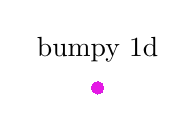
\begin{tikzpicture}

% defining custom colors
\definecolor{mycolor1}{rgb}{1,0.1,0.1}
\definecolor{mycolor2}{rgb}{0.1,1,0.1}
\definecolor{mycolor3}{rgb}{0.1,0.1,1}
\definecolor{mycolor4}{rgb}{0.4,0.4,0.1}
\definecolor{mycolor5}{rgb}{0.1,1,1}
\definecolor{mycolor6}{rgb}{0.9,0.1,0.9}


\begin{axis}[%
view={-72}{42},
xmin=0, xmax=100,
xlabel={Number of samples},
xmajorgrids,
y dir=reverse,
ymin=-5, ymax=5,
ylabel={sample location},
ymajorgrids,
zmin=0, zmax=0.4,
zmajorgrids,
axis lines=left,
scale only axis,
width=\fwidth,
height=\fheight,
title={bumpy 1d}]
\addplot3 [
color=mycolor1,
only marks,
mark=*,
mark options={solid}
]
coordinates{
 (1,1.80658755571437,0)(2,0.998800531788895,0)(3,0.00651006749742544,0)(4,1.81613919518463,0)(5,0.440580775765241,0)(6,0.449367687041336,0)(7,-0.256551471107748,0)(8,1.31558717205831,0)(9,-0.112021984403294,0)(10,1.07667055344516,0)(11,-1.16128577077944,0)(12,0.119369383719034,0)(13,0.320735845628267,0)(14,0.0402640667773458,0)(15,2.06327773390989,0)(16,0.255039339019574,0)(17,0.632936250357127,0)(18,0.617000279315325,0)(19,-0.853602168190745,0)(20,-1.06761291536516,0)(21,1.50307139720392,0)(22,-0.00840811186553614,0)(23,-1.31982773620949,0)(24,-0.111540127292066,0)(25,1.12311251982727,0)(26,1.40124400920854,0)(27,1.00557072236276,0)(28,1.21195074527836,0)(29,1.49797678338043,0)(30,-0.803785379507438,0)(31,1.5748486032612,0)(32,1.61514195647752,0)(33,0.915369817822849,0)(34,-0.465067544599383,0)(35,-0.447286151008213,0)(36,1.75185641279318,0)(37,1.77947668525513,0)(38,2.38964523124513,0)(39,-0.138060617270009,0)(40,-0.340981334817202,0)(41,0.410983748819743,0)(42,0.516195264786266,0)(43,2.07291736304994,0)(44,0.411659114650364,0)(45,-0.736980340944403,0)(46,0.60307901659922,0)(47,-0.487512671921799,0)(48,0.694183827581122,0)(49,1.33949190763838,0)(50,1.67854994074917,0)(51,0.749986875967693,0)(52,-1.36746542469219,0)(53,0.224329873788057,0)(54,2.40985437694474,0)(55,0.0117462674912602,0)(56,0.960138342637704,0)(57,1.5748118138742,0)(58,0.196846002558005,0)(59,0.896704830978507,0)(60,1.27015754979702,0)(61,2.13707241505252,0)(62,0.180619830895406,0)(63,2.65863159342433,0)(64,0.632229896405668,0)(65,0.220845411728789,0)(66,0.708892116739413,0)(67,1.79337568339899,0)(68,0.578487608331969,0)(69,0.437969403925056,0)(70,0.258682885020582,0)(71,0.39111069946538,0)(72,2.15544442179309,0)(73,2.36286567094005,0)(74,1.07343896167498,0)(75,0.365142143886078,0)(76,2.34496141170731,0)(77,2.26189670024877,0)(78,0.763532095055013,0)(79,1.67637926710673,0)(80,2.29703168411162,0)(81,0.608357000768451,0)(82,0.555998141980932,0)(83,0.88686131529198,0)(84,1.8472618216923,0)(85,-0.26676138235919,0)(86,0.0198282911037008,0)(87,0.937268784778228,0)(88,-0.407370578386672,0)(89,1.82767670940849,0)(90,3.56222699542744,0)(91,2.28106628798989,0)(92,2.41260583065085,0)(93,2.43851804562599,0)(94,-0.261085731755362,0)(95,0.41656609970833,0)(96,0.878713463466931,0)(97,0.851756701952996,0)(98,0.32893766112785,0)(99,1.86179396398578,0)(100,0.879633907088972,0) 
};

\addplot3 [
color=mycolor2,
only marks,
mark=*,
mark options={solid}
]
coordinates{
 (1,1.83783102716325,0)(2,1.55528470184943,0)(3,1.84499335290312,0)(4,1.69971223795818,0)(5,1.55720978833626,0)(6,1.19147610034437,0)(7,1.32289630334962,0)(8,1.00286685206184,0)(9,1.05873498649876,0)(10,0.406899192082884,0)(11,0.160042116212007,0)(12,-0.0231372932585992,0)(13,-0.295009666786,0)(14,0.0728510522654545,0)(15,-0.131103416725129,0)(16,-0.215556389658775,0)(17,-0.305048759114279,0)(18,-0.305048759114279,0)(19,-0.927262595726079,0)(20,-0.736554675039631,0)(21,-0.736554675039631,0)(22,-0.736554675039631,0)(23,-1.05643174972959,0)(24,-0.985877376014225,0)(25,-0.827370102752886,0)(26,-0.793985709063328,0)(27,-0.695338221776664,0)(28,-0.506241359438335,0)(29,-1.04502560377212,0)(30,-0.831619737563249,0)(31,-0.605471994281453,0)(32,-0.600611631127248,0)(33,-0.600611631127248,0)(34,-0.600611631127248,0)(35,-0.331230980742544,0)(36,-0.0531160333004192,0)(37,0.417951150333865,0)(38,0.417951150333865,0)(39,0.0255183951560275,0)(40,-0.129122121500634,0)(41,-0.129122121500634,0)(42,0.24178691593901,0)(43,0.0873599687102102,0)(44,0.0873599687102102,0)(45,-0.00653469055414106,0)(46,-0.445304723116025,0)(47,-0.510389511530183,0)(48,-0.371409967395221,0)(49,-0.12521085889957,0)(50,-0.172649173985513,0)(51,-0.889684699756346,0)(52,-0.889684699756346,0)(53,-0.412226823124366,0)(54,-0.693117316611722,0)(55,-0.674099902867446,0)(56,-0.460705670484238,0)(57,-0.683062488261129,0)(58,-0.684104512199444,0)(59,-0.567050417152866,0)(60,-0.175853770939754,0)(61,-0.403341754732515,0)(62,0.152786385302694,0)(63,0.0681100436369607,0)(64,-0.14665749459213,0)(65,-0.207091113583832,0)(66,0.0754190829911965,0)(67,-0.0262520623727157,0)(68,-0.172358965600923,0)(69,-0.172358965600923,0)(70,-0.333283892258858,0)(71,0.0637224926030731,0)(72,0.526321235707169,0)(73,0.581167451097927,0)(74,0.412030546122466,0)(75,0.868967465327205,0)(76,1.29963701639258,0)(77,1.25648207567882,0)(78,1.50199475689777,0)(79,1.94377496541913,0)(80,1.85154935129769,0)(81,1.74276641223068,0)(82,1.73861159531706,0)(83,2.03816208502386,0)(84,1.6691997396057,0)(85,1.3908650063902,0)(86,1.40265043094278,0)(87,0.989223553583419,0)(88,0.989223553583419,0)(89,0.989223553583419,0)(90,1.42595506055563,0)(91,1.90428302324639,0)(92,1.90428302324639,0)(93,1.53711547613937,0)(94,1.38424025383332,0)(95,1.37750885993924,0)(96,1.36225298957255,0)(97,1.36225298957255,0)(98,1.66639894617225,0)(99,1.6599586221085,0)(100,1.91687438464895,0) 
};

\addplot3 [
color=mycolor3,
only marks,
mark=*,
mark options={solid}
]
coordinates{
 (1,1.83783102716325,0)(2,1.55528470184943,0)(3,1.84499335290312,0)(4,1.69971223795818,0)(5,1.55720978833626,0)(6,1.19147610034437,0)(7,1.32289630334962,0)(8,1.00286685206184,0)(9,1.05873498649876,0)(10,0.406899192082884,0)(11,0.160042116212007,0)(12,-0.0231372932585992,0)(13,-0.295009666786,0)(14,0.0728510522654545,0)(15,-0.131103416725129,0)(16,-0.215556389658775,0)(17,-0.305048759114279,0)(18,-0.305048759114279,0)(19,-0.927262595726079,0)(20,-0.736554675039631,0)(21,-0.736554675039631,0)(22,-0.736554675039631,0)(23,-1.05643174972959,0)(24,-0.985877376014225,0)(25,-0.827370102752886,0)(26,-0.793985709063328,0)(27,-0.695338221776664,0)(28,-0.506241359438335,0)(29,-1.04502560377212,0)(30,-0.831619737563249,0)(31,-0.605471994281453,0)(32,-0.600611631127248,0)(33,-0.600611631127248,0)(34,-0.600611631127248,0)(35,-0.331230980742544,0)(36,-0.0531160333004192,0)(37,0.417951150333865,0)(38,0.417951150333865,0)(39,0.0255183951560275,0)(40,-0.129122121500634,0)(41,-0.129122121500634,0)(42,0.24178691593901,0)(43,0.0873599687102102,0)(44,0.0873599687102102,0)(45,-0.00653469055414106,0)(46,-0.445304723116025,0)(47,-0.510389511530183,0)(48,-0.371409967395221,0)(49,-0.12521085889957,0)(50,-0.172649173985513,0)(51,-0.889684699756346,0)(52,-0.889684699756346,0)(53,-0.412226823124366,0)(54,-0.693117316611722,0)(55,-0.674099902867446,0)(56,-0.460705670484238,0)(57,-0.683062488261129,0)(58,-0.684104512199444,0)(59,-0.567050417152866,0)(60,-0.175853770939754,0)(61,-0.403341754732515,0)(62,0.152786385302694,0)(63,0.0681100436369607,0)(64,-0.14665749459213,0)(65,-0.207091113583832,0)(66,0.0754190829911965,0)(67,-0.0262520623727157,0)(68,-0.172358965600923,0)(69,-0.172358965600923,0)(70,-0.333283892258858,0)(71,0.0637224926030731,0)(72,0.526321235707169,0)(73,0.581167451097927,0)(74,0.412030546122466,0)(75,0.868967465327205,0)(76,1.29963701639258,0)(77,1.25648207567882,0)(78,1.50199475689777,0)(79,1.94377496541913,0)(80,1.85154935129769,0)(81,1.74276641223068,0)(82,1.73861159531706,0)(83,2.03816208502386,0)(84,1.6691997396057,0)(85,1.3908650063902,0)(86,1.40265043094278,0)(87,0.989223553583419,0)(88,0.989223553583419,0)(89,0.989223553583419,0)(90,1.42595506055563,0)(91,1.90428302324639,0)(92,1.90428302324639,0)(93,1.53711547613937,0)(94,1.38424025383332,0)(95,1.37750885993924,0)(96,1.36225298957255,0)(97,1.36225298957255,0)(98,1.66639894617225,0)(99,1.6599586221085,0)(100,1.91687438464895,0) 
};

\addplot3 [
color=mycolor4,
only marks,
mark=*,
mark options={solid}
]
coordinates{
 (1,0,0)(2,-0.0722630014509791,0)(3,1.59220657523401,0)(4,0.197755900389233,0)(5,4.0463876976921,0)(6,2.11653093363423,0)(7,0.746390256836199,0)(8,2.97844603826185,0)(9,-2.22861557871095,0)(10,4.01308310538301,0)(11,0.789586316513189,0)(12,0.0351923307440427,0)(13,0.853226303417136,0)(14,0.242746915251778,0)(15,1.07528987040132,0)(16,0.0907020241323707,0)(17,0.789586316513189,0)(18,0.0351923307440427,0)(19,0.853226303417136,0)(20,0.242746915251778,0)(21,1.07528987040132,0)(22,0.0907020241323707,0)(23,-0.416507338688399,0)(24,1.63015961285643,0)(25,0.771261916071001,0)(26,0.789586316513189,0)(27,0.0351923307440427,0)(28,0.853226303417136,0)(29,0.242746915251778,0)(30,1.07528987040132,0)(31,0.0907020241323707,0)(32,-0.416507338688399,0)(33,1.63015961285643,0)(34,0.771261916071001,0)(35,2.88348313168541,0)(36,2.2184343839345,0)(37,0.811013178606619,0)(38,1.98191060610841,0)(39,1.23306186306595,0)(40,0.804709583014062,0)(41,0.789586316513189,0)(42,0.0351923307440427,0)(43,0.853226303417136,0)(44,0.242746915251778,0)(45,1.07528987040132,0)(46,0.0907020241323707,0)(47,-0.416507338688399,0)(48,1.63015961285643,0)(49,0.771261916071001,0)(50,2.88348313168541,0)(51,2.2184343839345,0)(52,0.811013178606619,0)(53,1.98191060610841,0)(54,1.23306186306595,0)(55,0.804709583014062,0)(56,1.84186443585223,0)(57,0.842580847347834,0)(58,-0.08353703384268,0)(59,0.415652489663906,0)(60,2.58249395877938,0)(61,-0.474607117680487,0)(62,0.971133308379448,0)(63,0.522485881853354,0)(64,0.789586316513189,0)(65,0.0351923307440427,0)(66,0.853226303417136,0)(67,0.242746915251778,0)(68,1.07528987040132,0)(69,0.0907020241323707,0)(70,-0.416507338688399,0)(71,1.63015961285643,0)(72,0.771261916071001,0)(73,2.88348313168541,0)(74,2.2184343839345,0)(75,0.811013178606619,0)(76,1.98191060610841,0)(77,1.23306186306595,0)(78,0.804709583014062,0)(79,1.84186443585223,0)(80,0.842580847347834,0)(81,-0.08353703384268,0)(82,0.415652489663906,0)(83,2.58249395877938,0)(84,-0.474607117680487,0)(85,0.971133308379448,0)(86,0.522485881853354,0)(87,-0.214329251278042,0)(88,0.930527460243513,0)(89,1.3089063111569,0)(90,2.20557234988212,0)(91,-0.154194462831529,0)(92,3.03327209711364,0)(93,0.75668100908,0)(94,1.22383266398528,0)(95,1.09905673231877,0)(96,1.44878152474525,0)(97,2.18602489450474,0)(98,1.86088328161285,0)(99,1.26903337092043,0)(100,1.05503737070021,0) 
};

\addplot3 [
color=mycolor5,
only marks,
mark=*,
mark options={solid}
]
coordinates{
 (1,1.80658755571437,0)(2,0.998800531788895,0)(3,0.00651006749742544,0)(4,1.81613919518463,0)(5,0.440580775765241,0)(6,0.449367687041336,0)(7,-0.256551471107748,0)(8,1.31558717205831,0)(9,-0.112021984403294,0)(10,1.07667055344516,0)(11,0,0)(12,-1.14594657440319,0)(13,-0.616168526087009,0)(14,0.712549368281365,0)(15,0.138718470241905,0)(16,2.45337658582799,0)(17,0.218209336164939,0)(18,0.546853976227813,0)(19,0.819606310351342,0)(20,-0.894591378617445,0)(21,-0.876760961426866,0)(22,1.51222411809321,0)(23,0.00399522635115273,0)(24,-1.51535303706221,0)(25,-0.109286243603495,0)(26,1.20399091703377,0)(27,1.64399732844031,0)(28,0.999531503263326,0)(29,1.25238235098803,0)(30,1.47642033115146,0)(31,-0.894386511001479,0)(32,1.56101555439251,0)(33,1.63646504917843,0)(34,0.868054218107654,0)(35,-0.448547079920989,0)(36,-0.448561952217575,0)(37,1.74905864673983,0)(38,1.76493935039812,0)(39,2.18476014145013,0)(40,-0.24045281825292,0)(41,-0.381829348682345,0)(42,0.506548718756328,0)(43,0.513326430931756,0)(44,2.04966687359209,0)(45,0.446710491959082,0)(46,-0.725203374522731,0)(47,0.513647705818216,0)(48,-0.546673845202187,0)(49,0.668984085400999,0)(50,1.31224405596341,0)(51,1.72175300081553,0)(52,0.768418907222412,0)(53,-1.34168941133323,0)(54,0.289697077722724,0)(55,2.31716728244177,0)(56,0.0697993084470579,0)(57,0.685315149721928,0)(58,1.59951626081611,0)(59,0.303468214486822,0)(60,0.87645226982307,0)(61,1.24049419404599,0)(62,2.24762194723401,0)(63,0.285457622952648,0)(64,2.72536652864443,0)(65,0.830801563203287,0)(66,0.222834694381501,0)(67,0.729955186370048,0)(68,1.72166038857147,0)(69,0.549579927808608,0)(70,0.448664475691728,0)(71,0.275056485864974,0)(72,0.275568664366949,0)(73,2.21393344246776,0)(74,2.24806357023684,0)(75,1.07350530262427,0)(76,0.224868666332245,0)(77,2.21516566226414,0)(78,2.24818601247864,0)(79,0.729698064081902,0)(80,1.66332979509496,0)(81,2.31696278991064,0)(82,0.514779221089341,0)(83,0.550038370328908,0)(84,0.870214925760818,0)(85,1.66284289395576,0)(86,-0.311412799091636,0)(87,-0.000218215974774869,0)(88,-1.78585287090431,0)(89,-0.392925049261162,0)(90,1.77034541235097,0)(91,2.99689081798096,0)(92,2.21557249432498,0)(93,3.26973560838496,0)(94,2.59377750926398,0)(95,-0.253853593600891,0)(96,0.449512403755979,0)(97,0.870326471095568,0)(98,0.832883013117596,0)(99,0.308989523620833,0)(100,2.31761076540514,0) 
};

\addplot3 [
color=mycolor6,
only marks,
mark=*,
mark options={solid}
]
coordinates{
 (1,1.83783102716325,0)(2,1.55528470184943,0)(3,1.84499335290312,0)(4,1.69971223795818,0)(5,1.55720978833626,0)(6,1.19147610034437,0)(7,1.32289630334962,0)(8,1.00286685206184,0)(9,1.05873498649876,0)(10,0.406899192082884,0)(11,0.160042116212007,0)(12,-0.0231372932585992,0)(13,-0.295009666786,0)(14,0.0728510522654545,0)(15,-0.131103416725129,0)(16,-0.215556389658775,0)(17,-0.305048759114279,0)(18,-0.305048759114279,0)(19,-0.927262595726079,0)(20,-0.736554675039631,0)(21,-0.736554675039631,0)(22,-0.736554675039631,0)(23,-1.05643174972959,0)(24,-0.985877376014225,0)(25,-0.827370102752886,0)(26,-0.793985709063328,0)(27,-0.695338221776664,0)(28,-0.506241359438335,0)(29,-1.04502560377212,0)(30,-0.831619737563249,0)(31,-0.605471994281453,0)(32,-0.600611631127248,0)(33,-0.600611631127248,0)(34,-0.600611631127248,0)(35,-0.331230980742544,0)(36,-0.0531160333004192,0)(37,0.417951150333865,0)(38,0.417951150333865,0)(39,0.0255183951560275,0)(40,-0.129122121500634,0)(41,-0.129122121500634,0)(42,0.24178691593901,0)(43,0.0873599687102102,0)(44,0.0873599687102102,0)(45,-0.00653469055414106,0)(46,-0.445304723116025,0)(47,-0.510389511530183,0)(48,-0.371409967395221,0)(49,-0.12521085889957,0)(50,-0.172649173985513,0)(51,-0.889684699756346,0)(52,-0.889684699756346,0)(53,-0.412226823124366,0)(54,-0.693117316611722,0)(55,-0.674099902867446,0)(56,-0.460705670484238,0)(57,-0.683062488261129,0)(58,-0.684104512199444,0)(59,-0.567050417152866,0)(60,-0.175853770939754,0)(61,-0.403341754732515,0)(62,0.152786385302694,0)(63,0.0681100436369607,0)(64,-0.14665749459213,0)(65,-0.207091113583832,0)(66,0.0754190829911965,0)(67,-0.0262520623727157,0)(68,-0.172358965600923,0)(69,-0.172358965600923,0)(70,-0.333283892258858,0)(71,0.0637224926030731,0)(72,0.526321235707169,0)(73,0.581167451097927,0)(74,0.412030546122466,0)(75,0.868967465327205,0)(76,1.29963701639258,0)(77,1.25648207567882,0)(78,1.50199475689777,0)(79,1.94377496541913,0)(80,1.85154935129769,0)(81,1.74276641223068,0)(82,1.73861159531706,0)(83,2.03816208502386,0)(84,1.6691997396057,0)(85,1.3908650063902,0)(86,1.40265043094278,0)(87,0.989223553583419,0)(88,0.989223553583419,0)(89,0.989223553583419,0)(90,1.42595506055563,0)(91,1.90428302324639,0)(92,1.90428302324639,0)(93,1.53711547613937,0)(94,1.38424025383332,0)(95,1.37750885993924,0)(96,1.36225298957255,0)(97,1.36225298957255,0)(98,1.66639894617225,0)(99,1.6599586221085,0)(100,1.91687438464895,0) 
};

\addplot3 [
color=black,
solid,
line width=2.0pt
]
coordinates{
 (101,-5,5.11081993411746e-08)(101,-4.98998998998999,5.39247442308828e-08)(101,-4.97997997997998,5.68913248336488e-08)(101,-4.96996996996997,6.00156398164438e-08)(101,-4.95995995995996,6.33057667195323e-08)(101,-4.94994994994995,6.6770179739441e-08)(101,-4.93993993993994,7.04177683020775e-08)(101,-4.92992992992993,7.42578564588783e-08)(101,-4.91991991991992,7.8300223140139e-08)(101,-4.90990990990991,8.25551233009881e-08)(101,-4.8998998998999,8.7033309996806e-08)(101,-4.88988988988989,9.1746057426298e-08)(101,-4.87987987987988,9.67051849818651e-08)(101,-4.86986986986987,1.01923082348423e-07)(101,-4.85985985985986,1.07412735693343e-07)(101,-4.84984984984985,1.131877549918e-07)(101,-4.83983983983984,1.19262402533461e-07)(101,-4.82982982982983,1.25651622658131e-07)(101,-4.81981981981982,1.32371072769752e-07)(101,-4.80980980980981,1.39437155679971e-07)(101,-4.7997997997998,1.46867053334327e-07)(101,-4.78978978978979,1.5467876197611e-07)(101,-4.77977977977978,1.62891128804875e-07)(101,-4.76976976976977,1.71523890188706e-07)(101,-4.75975975975976,1.80597711491431e-07)(101,-4.74974974974975,1.90134228578186e-07)(101,-4.73973973973974,2.00156091064989e-07)(101,-4.72972972972973,2.1068700738034e-07)(101,-4.71971971971972,2.21751791709245e-07)(101,-4.70970970970971,2.33376412892543e-07)(101,-4.6996996996997,2.45588045357023e-07)(101,-4.68968968968969,2.58415122154387e-07)(101,-4.67967967967968,2.71887390189872e-07)(101,-4.66966966966967,2.86035967724152e-07)(101,-4.65965965965966,3.00893404234997e-07)(101,-4.64964964964965,3.16493742728137e-07)(101,-4.63963963963964,3.32872584589879e-07)(101,-4.62962962962963,3.5006715707711e-07)(101,-4.61961961961962,3.681163835436e-07)(101,-4.60960960960961,3.87060956504849e-07)(101,-4.5995995995996,4.06943413647142e-07)(101,-4.58958958958959,4.2780821688998e-07)(101,-4.57957957957958,4.4970183461476e-07)(101,-4.56956956956957,4.72672827176209e-07)(101,-4.55955955955956,4.9677193581697e-07)(101,-4.54954954954955,5.22052175109697e-07)(101,-4.53953953953954,5.48568929055003e-07)(101,-4.52952952952953,5.76380050967807e-07)(101,-4.51951951951952,6.05545967288918e-07)(101,-4.50950950950951,6.36129785463041e-07)(101,-4.4994994994995,6.68197406028908e-07)(101,-4.48948948948949,7.01817639071892e-07)(101,-4.47947947947948,7.37062325194204e-07)(101,-4.46946946946947,7.74006461162573e-07)(101,-4.45945945945946,8.12728330398438e-07)(101,-4.44944944944945,8.53309638480717e-07)(101,-4.43943943943944,8.95835653836442e-07)(101,-4.42942942942943,9.4039535380009e-07)(101,-4.41941941941942,9.87081576227803e-07)(101,-4.40940940940941,1.03599117685841e-06)(101,-4.3993993993994,1.08722519261902e-06)(101,-4.38938938938939,1.14088901107883e-06)(101,-4.37937937937938,1.19709254626088e-06)(101,-4.36936936936937,1.25595042102768e-06)(101,-4.35935935935936,1.31758215626328e-06)(101,-4.34934934934935,1.38211236708027e-06)(101,-4.33933933933934,1.44967096628772e-06)(101,-4.32932932932933,1.52039337536206e-06)(101,-4.31931931931932,1.59442074317044e-06)(101,-4.30930930930931,1.67190017270311e-06)(101,-4.2992992992993,1.75298495607845e-06)(101,-4.28928928928929,1.83783481809205e-06)(101,-4.27927927927928,1.92661616858863e-06)(101,-4.26926926926927,2.01950236394344e-06)(101,-4.25925925925926,2.11667397794776e-06)(101,-4.24924924924925,2.21831908240112e-06)(101,-4.23923923923924,2.32463353772121e-06)(101,-4.22922922922923,2.43582129389097e-06)(101,-4.21921921921922,2.55209470207066e-06)(101,-4.20920920920921,2.67367483721183e-06)(101,-4.1991991991992,2.80079183201889e-06)(101,-4.18918918918919,2.93368522261295e-06)(101,-4.17917917917918,3.07260430626219e-06)(101,-4.16916916916917,3.21780851155235e-06)(101,-4.15915915915916,3.36956778138026e-06)(101,-4.14914914914915,3.52816296916362e-06)(101,-4.13913913913914,3.69388624866996e-06)(101,-4.12912912912913,3.86704153787763e-06)(101,-4.11911911911912,4.04794493729243e-06)(101,-4.10910910910911,4.23692518315371e-06)(101,-4.0990990990991,4.43432411597417e-06)(101,-4.08908908908909,4.640497164869e-06)(101,-4.07907907907908,4.85581384814053e-06)(101,-4.06906906906907,5.08065829059558e-06)(101,-4.05905905905906,5.31542975808455e-06)(101,-4.04904904904905,5.56054320976244e-06)(101,-4.03903903903904,5.81642986858316e-06)(101,-4.02902902902903,6.08353781055134e-06)(101,-4.01901901901902,6.3623325732668e-06)(101,-4.00900900900901,6.65329778430931e-06)(101,-3.998998998999,6.95693581002364e-06)(101,-3.98898898898899,7.27376842527704e-06)(101,-3.97897897897898,7.60433750477391e-06)(101,-3.96896896896897,7.94920573652506e-06)(101,-3.95895895895896,8.30895735808191e-06)(101,-3.94894894894895,8.68419891615835e-06)(101,-3.93893893893894,9.07556005027689e-06)(101,-3.92892892892893,9.4836943010883e-06)(101,-3.91891891891892,9.90927994402685e-06)(101,-3.90890890890891,1.03530208489778e-05)(101,-3.8988988988989,1.08156473666464e-05)(101,-3.88888888888889,1.12979172423307e-05)(101,-3.87887887887888,1.18006165578159e-05)(101,-3.86886886886887,1.232456070212e-05)(101,-3.85885885885886,1.28705953718348e-05)(101,-3.84884884884885,1.34395976018207e-05)(101,-3.83883883883884,1.40324768270271e-05)(101,-3.82882882882883,1.46501759762241e-05)(101,-3.81881881881882,1.52936725984456e-05)(101,-3.80880880880881,1.5963980022958e-05)(101,-3.7987987987988,1.66621485535812e-05)(101,-3.78878878878879,1.73892666982059e-05)(101,-3.77877877877878,1.8146462434361e-05)(101,-3.76876876876877,1.89349045117025e-05)(101,-3.75875875875876,1.9755803792307e-05)(101,-3.74874874874875,2.06104146296689e-05)(101,-3.73873873873874,2.15000362873099e-05)(101,-3.72872872872873,2.24260143979306e-05)(101,-3.71871871871872,2.33897424640398e-05)(101,-3.70870870870871,2.43926634010146e-05)(101,-3.6986986986987,2.54362711235598e-05)(101,-3.68868868868869,2.65221121765426e-05)(101,-3.67867867867868,2.7651787411198e-05)(101,-3.66866866866867,2.88269537077078e-05)(101,-3.65865865865866,3.00493257451746e-05)(101,-3.64864864864865,3.13206778200181e-05)(101,-3.63863863863864,3.26428457138395e-05)(101,-3.62862862862863,3.40177286118086e-05)(101,-3.61861861861862,3.54472910726394e-05)(101,-3.60860860860861,3.69335650512342e-05)(101,-3.5985985985986,3.84786519750866e-05)(101,-3.58858858858859,4.00847248755399e-05)(101,-3.57857857857858,4.17540305750184e-05)(101,-3.56856856856857,4.34888919313471e-05)(101,-3.55855855855856,4.52917101402936e-05)(101,-3.54854854854855,4.7164967097471e-05)(101,-3.53853853853854,4.91112278207536e-05)(101,-3.52852852852853,5.11331429343566e-05)(101,-3.51851851851852,5.32334512157526e-05)(101,-3.50850850850851,5.54149822065914e-05)(101,-3.4984984984985,5.76806588888031e-05)(101,-3.48848848848849,6.00335004270721e-05)(101,-3.47847847847848,6.247662497887e-05)(101,-3.46846846846847,6.50132525732432e-05)(101,-3.45845845845846,6.76467080595536e-05)(101,-3.44844844844845,7.038042412738e-05)(101,-3.43843843843844,7.32179443987761e-05)(101,-3.42842842842843,7.61629265941018e-05)(101,-3.41841841841842,7.92191457726318e-05)(101,-3.40840840840841,8.23904976491468e-05)(101,-3.3983983983984,8.56810019877199e-05)(101,-3.38838838838839,8.90948060739029e-05)(101,-3.37837837837838,9.26361882665113e-05)(101,-3.36836836836837,9.63095616302123e-05)(101,-3.35835835835836,0.000100119477650111)(101,-3.34834834834835,0.000104070630029518)(101,-3.33833833833834,0.000108167858572083)(101,-3.32832832832833,0.000112416153149481)(101,-3.31831831831832,0.000116820657755785)(101,-3.30830830830831,0.00012138667464972)(101,-3.2982982982983,0.000126119668585905)(101,-3.28828828828829,0.000131025271136235)(101,-3.27827827827828,0.000136109285102509)(101,-3.26826826826827,0.00014137768902141)(101,-3.25825825825826,0.000146836641762907)(101,-3.24824824824825,0.000152492487223157)(101,-3.23823823823824,0.000158351759112941)(101,-3.22822822822823,0.000164421185842662)(101,-3.21821821821822,0.000170707695504897)(101,-3.20820820820821,0.000177218420955482)(101,-3.1981981981982,0.00018396070499407)(101,-3.18818818818819,0.000190942105645091)(101,-3.17817817817818,0.000198170401539993)(101,-3.16816816816817,0.000205653597401617)(101,-3.15815815815816,0.000213399929631547)(101,-3.14814814814815,0.000221417872001199)(101,-3.13813813813814,0.000229716141447411)(101,-3.12812812812813,0.000238303703973239)(101,-3.11811811811812,0.000247189780654635)(101,-3.10810810810811,0.000256383853753615)(101,-3.0980980980981,0.00026589567293851)(101,-3.08808808808809,0.000275735261611827)(101,-3.07807807807808,0.000285912923346188)(101,-3.06806806806807,0.000296439248428802)(101,-3.05805805805806,0.000307325120514806)(101,-3.04804804804805,0.000318581723389829)(101,-3.03803803803804,0.000330220547842006)(101,-3.02802802802803,0.000342253398643658)(101,-3.01801801801802,0.000354692401642761)(101,-3.00800800800801,0.000367550010964257)(101,-2.997997997998,0.000380839016321237)(101,-2.98798798798799,0.00039457255043588)(101,-2.97797797797798,0.000408764096570028)(101,-2.96796796796797,0.000423427496165156)(101,-2.95795795795796,0.000438576956591439)(101,-2.94794794794795,0.000454227059005526)(101,-2.93793793793794,0.000470392766316549)(101,-2.92792792792793,0.000487089431259813)(101,-2.91791791791792,0.000504332804577509)(101,-2.90790790790791,0.000522139043305726)(101,-2.8978978978979,0.000540524719166906)(101,-2.88788788788789,0.000559506827066819)(101,-2.87787787787788,0.000579102793695029)(101,-2.86786786786787,0.000599330486227695)(101,-2.85785785785786,0.000620208221131474)(101,-2.84784784784785,0.000641754773067176)(101,-2.83783783783784,0.000663989383891688)(101,-2.82782782782783,0.000686931771756599)(101,-2.81781781781782,0.000710602140301833)(101,-2.80780780780781,0.000735021187942446)(101,-2.7977977977978,0.000760210117246659)(101,-2.78778778778779,0.000786190644403083)(101,-2.77777777777778,0.000812985008774878)(101,-2.76776776776777,0.000840615982538572)(101,-2.75775775775776,0.000869106880405052)(101,-2.74774774774775,0.00089848156942012)(101,-2.73773773773774,0.000928764478841885)(101,-2.72772772772773,0.000959980610092101)(101,-2.71771771771772,0.000992155546778408)(101,-2.70770770770771,0.00102531546478432)(101,-2.6976976976977,0.00105948714242363)(101,-2.68768768768769,0.00109469797065569)(101,-2.67767767767768,0.00113097596335804)(101,-2.66766766766767,0.00116834976765247)(101,-2.65765765765766,0.00120684867428064)(101,-2.64764764764765,0.00124650262802509)(101,-2.63763763763764,0.00128734223817133)(101,-2.62762762762763,0.0013293987890067)(101,-2.61761761761762,0.00137270425035111)(101,-2.60760760760761,0.00141729128811515)(101,-2.5975975975976,0.00146319327488038)(101,-2.58758758758759,0.00151044430049673)(101,-2.57757757757758,0.00155907918269173)(101,-2.56756756756757,0.00160913347768595)(101,-2.55755755755756,0.00166064349080907)(101,-2.54754754754755,0.0017136462871106)(101,-2.53753753753754,0.0017681797019593)(101,-2.52752752752753,0.00182428235162492)(101,-2.51751751751752,0.00188199364383595)(101,-2.50750750750751,0.00194135378830667)(101,-2.4974974974975,0.00200240380722678)(101,-2.48748748748749,0.00206518554570639)(101,-2.47747747747748,0.00212974168216944)(101,-2.46746746746747,0.00219611573868801)(101,-2.45745745745746,0.0022643520912499)(101,-2.44744744744745,0.00233449597995175)(101,-2.43743743743744,0.00240659351910981)(101,-2.42742742742743,0.00248069170727998)(101,-2.41741741741742,0.00255683843717888)(101,-2.40740740740741,0.00263508250549754)(101,-2.3973973973974,0.00271547362259854)(101,-2.38738738738739,0.00279806242208813)(101,-2.37737737737738,0.00288290047025379)(101,-2.36736736736737,0.00297004027535818)(101,-2.35735735735736,0.00305953529677974)(101,-2.34734734734735,0.00315143995399044)(101,-2.33733733733734,0.00324580963536052)(101,-2.32732732732733,0.00334270070678032)(101,-2.31731731731732,0.00344217052008891)(101,-2.30730730730731,0.00354427742129893)(101,-2.2972972972973,0.00364908075860708)(101,-2.28728728728729,0.00375664089017954)(101,-2.27727727727728,0.00386701919170111)(101,-2.26726726726727,0.00398027806367701)(101,-2.25725725725726,0.00409648093847614)(101,-2.24724724724725,0.00421569228710397)(101,-2.23723723723724,0.0043379776256937)(101,-2.22722722722723,0.00446340352170372)(101,-2.21721721721722,0.00459203759980943)(101,-2.20720720720721,0.00472394854747712)(101,-2.1971971971972,0.00485920612020806)(101,-2.18718718718719,0.0049978811464398)(101,-2.17717717717718,0.00514004553209264)(101,-2.16716716716717,0.00528577226474827)(101,-2.15715715715716,0.00543513541744791)(101,-2.14714714714715,0.00558821015209692)(101,-2.13713713713714,0.00574507272246302)(101,-2.12712712712713,0.00590580047675471)(101,-2.11711711711712,0.00607047185976689)(101,-2.10710710710711,0.0062391664145802)(101,-2.0970970970971,0.00641196478380062)(101,-2.08708708708709,0.00658894871032608)(101,-2.07707707707708,0.00677020103762612)(101,-2.06706706706707,0.0069558057095212)(101,-2.05705705705706,0.00714584776944816)(101,-2.04704704704705,0.00734041335919751)(101,-2.03703703703704,0.00753958971710945)(101,-2.02702702702703,0.0077434651757144)(101,-2.01701701701702,0.0079521291588043)(101,-2.00700700700701,0.00816567217792099)(101,-1.996996996997,0.00838418582824773)(101,-1.98698698698699,0.00860776278389006)(101,-1.97697697697698,0.00883649679253226)(101,-1.96696696696697,0.0090704826694557)(101,-1.95695695695696,0.00930981629090521)(101,-1.94694694694695,0.00955459458679001)(101,-1.93693693693694,0.00980491553270555)(101,-1.92692692692693,0.0100608781412627)(101,-1.91691691691692,0.0103225824527109)(101,-1.90690690690691,0.0105901295248422)(101,-1.8968968968969,0.0108636214221624)(101,-1.88688688688689,0.0111431612043171)(101,-1.87687687687688,0.0114288529137591)(101,-1.86686686686687,0.0117208015626442)(101,-1.85685685685686,0.0120191131189437)(101,-1.84684684684685,0.0123238944917605)(101,-1.83683683683684,0.0126352535158368)(101,-1.82682682682683,0.0129532989352406)(101,-1.81681681681682,0.0132781403862217)(101,-1.80680680680681,0.0136098883792217)(101,-1.7967967967968,0.0139486542800312)(101,-1.78678678678679,0.0142945502900789)(101,-1.77677677677678,0.0146476894258455)(101,-1.76676676676677,0.0150081854973896)(101,-1.75675675675676,0.015376153085976)(101,-1.74674674674675,0.0157517075207978)(101,-1.73673673673674,0.0161349648547808)(101,-1.72672672672673,0.0165260418394633)(101,-1.71671671671672,0.0169250558989407)(101,-1.70670670670671,0.0173321251028675)(101,-1.6966966966967,0.0177473681385093)(101,-1.68668668668669,0.018170904281836)(101,-1.67667667667668,0.0186028533676497)(101,-1.66666666666667,0.0190433357587419)(101,-1.65665665665666,0.0194924723140716)(101,-1.64664664664665,0.0199503843559603)(101,-1.63663663663664,0.0204171936362984)(101,-1.62662662662663,0.0208930223017582)(101,-1.61661661661662,0.0213779928580092)(101,-1.60660660660661,0.0218722281329328)(101,-1.5965965965966,0.0223758512388325)(101,-1.58658658658659,0.0228889855336385)(101,-1.57657657657658,0.0234117545811032)(101,-1.56656656656657,0.0239442821099876)(101,-1.55655655655656,0.0244866919722379)(101,-1.54654654654655,0.0250391081001521)(101,-1.53653653653654,0.0256016544625367)(101,-1.52652652652653,0.0261744550198564)(101,-1.51651651651652,0.0267576336783773)(101,-1.50650650650651,0.0273513142433071)(101,-1.4964964964965,0.0279556203709362)(101,-1.48648648648649,0.0285706755197821)(101,-1.47647647647648,0.0291966029007447)(101,-1.46646646646647,0.0298335254262754)(101,-1.45645645645646,0.0304815656585686)(101,-1.44644644644645,0.0311408457567812)(101,-1.43643643643644,0.0318114874232894)(101,-1.42642642642643,0.03249361184899)(101,-1.41641641641642,0.0331873396576579)(101,-1.40640640640641,0.0338927908493678)(101,-1.3963963963964,0.0346100847429932)(101,-1.38638638638639,0.0353393399177936)(101,-1.37637637637638,0.0360806741541035)(101,-1.36636636636637,0.0368342043731365)(101,-1.35635635635636,0.0376000465759191)(101,-1.34634634634635,0.0383783157813702)(101,-1.33633633633634,0.0391691259635421)(101,-1.32632632632633,0.0399725899880398)(101,-1.31631631631632,0.0407888195476381)(101,-1.30630630630631,0.0416179250971146)(101,-1.2962962962963,0.0424600157873179)(101,-1.28628628628629,0.0433151993984932)(101,-1.27627627627628,0.0441835822728858)(101,-1.26626626626627,0.0450652692466461)(101,-1.25625625625626,0.0459603635810582)(101,-1.24624624624625,0.0468689668931186)(101,-1.23623623623624,0.047791179085488)(101,-1.22622622622623,0.0487270982758443)(101,-1.21621621621622,0.0496768207256629)(101,-1.20620620620621,0.0506404407684523)(101,-1.1961961961962,0.0516180507374753)(101,-1.18618618618619,0.0526097408929834)(101,-1.17617617617618,0.053615599348997)(101,-1.16616616616617,0.0546357119996626)(101,-1.15615615615616,0.0556701624452183)(101,-1.14614614614615,0.0567190319176032)(101,-1.13613613613614,0.0577823992057425)(101,-1.12612612612613,0.0588603405805454)(101,-1.11611611611612,0.0599529297196508)(101,-1.10610610610611,0.0610602376319567)(101,-1.0960960960961,0.0621823325819738)(101,-1.08608608608609,0.0633192800140383)(101,-1.07607607607608,0.0644711424764251)(101,-1.06606606606607,0.065637979545401)(101,-1.05605605605606,0.0668198477492589)(101,-1.04604604604605,0.0680168004923745)(101,-1.03603603603604,0.0692288879793261)(101,-1.02602602602603,0.0704561571391243)(101,-1.01601601601602,0.0716986515495911)(101,-1.00600600600601,0.0729564113619356)(101,-0.995995995995996,0.0742294732255705)(101,-0.985985985985986,0.075517870213214)(101,-0.975975975975976,0.076821631746326)(101,-0.965965965965966,0.0781407835209231)(101,-0.955955955955956,0.0794753474338202)(101,-0.945945945945946,0.0808253415093486)(101,-0.935935935935936,0.0821907798265965)(101,-0.925925925925926,0.0835716724472234)(101,-0.915915915915916,0.0849680253438959)(101,-0.905905905905906,0.0863798403293959)(101,-0.895895895895896,0.0878071149864522)(101,-0.885885885885886,0.089249842598344)(101,-0.875875875875876,0.0907080120803301)(101,-0.865865865865866,0.0921816079119533)(101,-0.855855855855856,0.093670610070272)(101,-0.845845845845846,0.0951749939640724)(101,-0.835835835835836,0.0966947303691108)(101,-0.825825825825826,0.0982297853644411)(101,-0.815815815815816,0.0997801202698778)(101,-0.805805805805806,0.101345691584649)(101,-0.795795795795796,0.102926450927289)(101,-0.785785785785786,0.104522344976829)(101,-0.775775775775776,0.106133315415332)(101,-0.765765765765765,0.107759298871824)(101,-0.755755755755755,0.10940022686769)(101,-0.745745745745745,0.111056025763558)(101,-0.735735735735735,0.112726616707754)(101,-0.725725725725725,0.114411915586356)(101,-0.715715715715715,0.116111832974919)(101,-0.705705705705705,0.117826274091901)(101,-0.695695695695695,0.119555138753866)(101,-0.685685685685685,0.121298321332489)(101,-0.675675675675675,0.123055710713434)(101,-0.665665665665665,0.124827190257145)(101,-0.655655655655655,0.126612637761601)(101,-0.645645645645645,0.128411925427089)(101,-0.635635635635635,0.130224919823028)(101,-0.625625625625625,0.132051481856919)(101,-0.615615615615615,0.133891466745435)(101,-0.605605605605605,0.135744723987727)(101,-0.595595595595595,0.137611097340974)(101,-0.585585585585585,0.139490424798223)(101,-0.575575575575575,0.141382538568572)(101,-0.565565565565565,0.143287265059733)(101,-0.555555555555555,0.145204424863015)(101,-0.545545545545545,0.147133832740771)(101,-0.535535535535535,0.149075297616351)(101,-0.525525525525525,0.151028622566596)(101,-0.515515515515515,0.152993604816915)(101,-0.505505505505505,0.154970035738977)(101,-0.495495495495495,0.156957700851058)(101,-0.485485485485485,0.158956379821074)(101,-0.475475475475475,0.160965846472335)(101,-0.465465465465465,0.162985868792053)(101,-0.455455455455455,0.165016208942631)(101,-0.445445445445445,0.167056623275763)(101,-0.435435435435435,0.169106862349372)(101,-0.425425425425425,0.17116667094742)(101,-0.415415415415415,0.173235788102597)(101,-0.405405405405405,0.175313947121934)(101,-0.395395395395395,0.17740087561534)(101,-0.385385385385385,0.179496295527099)(101,-0.375375375375375,0.181599923170336)(101,-0.365365365365365,0.183711469264476)(101,-0.355355355355355,0.185830638975701)(101,-0.345345345345345,0.187957131960421)(101,-0.335335335335335,0.190090642411784)(101,-0.325325325325325,0.192230859109207)(101,-0.315315315315315,0.194377465470964)(101,-0.305305305305305,0.196530139609814)(101,-0.295295295295295,0.198688554391694)(101,-0.285285285285285,0.200852377497451)(101,-0.275275275275275,0.203021271487647)(101,-0.265265265265265,0.205194893870404)(101,-0.255255255255255,0.207372897172306)(101,-0.245245245245245,0.209554929012339)(101,-0.235235235235235,0.21174063217887)(101,-0.225225225225225,0.213929644709649)(101,-0.215215215215215,0.216121599974822)(101,-0.205205205205205,0.218316126762952)(101,-0.195195195195195,0.220512849370005)(101,-0.185185185185185,0.222711387691321)(101,-0.175175175175175,0.224911357316513)(101,-0.165165165165165,0.227112369627294)(101,-0.155155155155155,0.229314031898199)(101,-0.145145145145145,0.231515947400177)(101,-0.135135135135135,0.233717715507026)(101,-0.125125125125125,0.235918931804637)(101,-0.115115115115115,0.238119188203013)(101,-0.105105105105105,0.24031807305103)(101,-0.0950950950950951,0.242515171253913)(101,-0.0850850850850851,0.24471006439336)(101,-0.075075075075075,0.246902330850308)(101,-0.065065065065065,0.249091545930266)(101,-0.055055055055055,0.251277281991193)(101,-0.045045045045045,0.25345910857386)(101,-0.035035035035035,0.255636592534648)(101,-0.025025025025025,0.257809298180739)(101,-0.015015015015015,0.25997678740764)(101,-0.005005005005005,0.262138619838973)(101,0.005005005005005,0.264294352968507)(101,0.015015015015015,0.26644354230433)(101,0.025025025025025,0.268585741515139)(101,0.035035035035035,0.270720502578553)(101,0.045045045045045,0.272847375931408)(101,0.055055055055055,0.274965910621957)(101,0.065065065065065,0.277075654463898)(101,0.075075075075075,0.279176154192186)(101,0.0850850850850851,0.281266955620525)(101,0.0950950950950951,0.283347603800492)(101,0.105105105105105,0.285417643182202)(101,0.115115115115115,0.287476617776452)(101,0.125125125125125,0.289524071318249)(101,0.135135135135135,0.291559547431654)(101,0.145145145145145,0.293582589795863)(101,0.155155155155155,0.295592742312432)(101,0.165165165165165,0.29758954927357)(101,0.175175175175175,0.299572555531413)(101,0.185185185185185,0.3015413066682)(101,0.195195195195195,0.303495349167244)(101,0.205205205205205,0.305434230584635)(101,0.215215215215215,0.307357499721565)(101,0.225225225225225,0.309264706797202)(101,0.235235235235235,0.311155403621998)(101,0.245245245245245,0.313029143771372)(101,0.255255255255255,0.314885482759639)(101,0.265265265265265,0.316723978214123)(101,0.275275275275275,0.318544190049331)(101,0.285285285285285,0.320345680641122)(101,0.295295295295295,0.322128015000751)(101,0.305305305305305,0.323890760948702)(101,0.315315315315315,0.325633489288218)(101,0.325325325325325,0.327355773978424)(101,0.335335335335335,0.329057192306945)(101,0.345345345345345,0.33073732506193)(101,0.355355355355355,0.332395756703377)(101,0.365365365365365,0.334032075533667)(101,0.375375375375375,0.335645873867197)(101,0.385385385385385,0.337236748199039)(101,0.395395395395395,0.338804299372501)(101,0.405405405405405,0.34034813274551)(101,0.415415415415415,0.341867858355713)(101,0.425425425425425,0.343363091084204)(101,0.435435435435435,0.344833450817776)(101,0.445445445445445,0.346278562609611)(101,0.455455455455455,0.347698056838297)(101,0.465465465465465,0.349091569365099)(101,0.475475475475475,0.350458741689375)(101,0.485485485485485,0.351799221102047)(101,0.495495495495495,0.353112660837041)(101,0.505505505505505,0.354398720220603)(101,0.515515515515515,0.355657064818391)(101,0.525525525525525,0.356887366580273)(101,0.535535535535535,0.358089303982724)(101,0.545545545545545,0.359262562168752)(101,0.555555555555555,0.360406833085256)(101,0.565565565565565,0.361521815617737)(101,0.575575575575575,0.362607215722281)(101,0.585585585585585,0.36366274655473)(101,0.595595595595595,0.364688128596959)(101,0.605605605605605,0.365683089780195)(101,0.615615615615615,0.366647365605282)(101,0.625625625625625,0.36758069925983)(101,0.635635635635635,0.368482841732179)(101,0.645645645645645,0.369353551922089)(101,0.655655655655655,0.370192596748114)(101,0.665665665665665,0.370999751251563)(101,0.675675675675675,0.371774798697015)(101,0.685685685685685,0.37251753066929)(101,0.695695695695695,0.373227747166849)(101,0.705705705705705,0.373905256691545)(101,0.715715715715715,0.374549876334665)(101,0.725725725725725,0.37516143185923)(101,0.735735735735735,0.375739757778475)(101,0.745745745745745,0.376284697430485)(101,0.755755755755755,0.376796103048913)(101,0.765765765765765,0.377273835829763)(101,0.775775775775776,0.377717765994173)(101,0.785785785785786,0.378127772847174)(101,0.795795795795796,0.378503744832376)(101,0.805805805805806,0.378845579582554)(101,0.815815815815816,0.379153183966102)(101,0.825825825825826,0.379426474129318)(101,0.835835835835836,0.379665375534499)(101,0.845845845845846,0.379869822993829)(101,0.855855855855856,0.380039760699017)(101,0.865865865865866,0.380175142246689)(101,0.875875875875876,0.380275930659508)(101,0.885885885885886,0.380342098403002)(101,0.895895895895896,0.380373627398104)(101,0.905905905905906,0.380370509029381)(101,0.915915915915916,0.380332744148963)(101,0.925925925925926,0.380260343076151)(101,0.935935935935936,0.380153325592716)(101,0.945945945945946,0.380011720933897)(101,0.955955955955956,0.379835567775085)(101,0.965965965965966,0.379624914214222)(101,0.975975975975976,0.379379817749909)(101,0.985985985985986,0.379100345255254)(101,0.995995995995996,0.378786572947463)(101,1.00600600600601,0.378438586353194)(101,1.01601601601602,0.378056480269707)(101,1.02602602602603,0.377640358721824)(101,1.03603603603604,0.377190334914733)(101,1.04604604604605,0.376706531182658)(101,1.05605605605606,0.376189078933439)(101,1.06606606606607,0.375638118589045)(101,1.07607607607608,0.375053799522068)(101,1.08608608608609,0.374436279988231)(101,1.0960960960961,0.373785727054956)(101,1.10610610610611,0.373102316526039)(101,1.11611611611612,0.372386232862473)(101,1.12612612612613,0.371637669099475)(101,1.13613613613614,0.37085682675977)(101,1.14614614614615,0.370043915763176)(101,1.15615615615616,0.369199154332566)(101,1.16616616616617,0.368322768896243)(101,1.17617617617618,0.367414993986811)(101,1.18618618618619,0.366476072136585)(101,1.1961961961962,0.365506253769621)(101,1.20620620620621,0.364505797090432)(101,1.21621621621622,0.363474967969442)(101,1.22622622622623,0.362414039825273)(101,1.23623623623624,0.361323293503922)(101,1.24624624624625,0.360203017154908)(101,1.25625625625626,0.359053506104467)(101,1.26626626626627,0.357875062725866)(101,1.27627627627628,0.356667996306926)(101,1.28628628628629,0.355432622914828)(101,1.2962962962963,0.354169265258286)(101,1.30630630630631,0.352878252547168)(101,1.31631631631632,0.351559920349664)(101,1.32632632632633,0.35021461044707)(101,1.33633633633634,0.34884267068628)(101,1.34634634634635,0.34744445483009)(101,1.35635635635636,0.346020322405384)(101,1.36636636636637,0.344570638549303)(101,1.37637637637638,0.343095773853489)(101,1.38638638638639,0.341596104206499)(101,1.3963963963964,0.340072010634468)(101,1.40640640640641,0.338523879140143)(101,1.41641641641642,0.336952100540349)(101,1.42642642642643,0.335357070302013)(101,1.43643643643644,0.333739188376826)(101,1.44644644644645,0.332098859034637)(101,1.45645645645646,0.330436490695686)(101,1.46646646646647,0.328752495761768)(101,1.47647647647648,0.32704729044643)(101,1.48648648648649,0.325321294604279)(101,1.4964964964965,0.323574931559536)(101,1.50650650650651,0.32180862793389)(101,1.51651651651652,0.320022813473783)(101,1.52652652652653,0.31821792087721)(101,1.53653653653654,0.316394385620123)(101,1.54654654654655,0.314552645782556)(101,1.55655655655656,0.312693141874549)(101,1.56656656656657,0.310816316661974)(101,1.57657657657658,0.308922614992363)(101,1.58658658658659,0.307012483620822)(101,1.5965965965966,0.305086371036135)(101,1.60660660660661,0.303144727287151)(101,1.61661661661662,0.30118800380954)(101,1.62662662662663,0.299216653253011)(101,1.63663663663664,0.297231129309096)(101,1.64664664664665,0.295231886539573)(101,1.65665665665666,0.293219380205624)(101,1.66666666666667,0.291194066097822)(101,1.67667667667668,0.289156400367029)(101,1.68668668668669,0.28710683935628)(101,1.6966966966967,0.285045839433766)(101,1.70670670670671,0.282973856826967)(101,1.71671671671672,0.280891347458038)(101,1.72672672672673,0.278798766780524)(101,1.73673673673674,0.276696569617479)(101,1.74674674674675,0.274585210001072)(101,1.75675675675676,0.272465141013748)(101,1.76676676676677,0.270336814631037)(101,1.77677677677678,0.268200681566057)(101,1.78678678678679,0.266057191115808)(101,1.7967967967968,0.263906791009313)(101,1.80680680680681,0.261749927257673)(101,1.81681681681682,0.259587044006111)(101,1.82682682682683,0.257418583388064)(101,1.83683683683684,0.255244985381388)(101,1.84684684684685,0.253066687666727)(101,1.85685685685686,0.250884125488125)(101,1.86686686686687,0.248697731515919)(101,1.87687687687688,0.246507935711974)(101,1.88688688688689,0.244315165197322)(101,1.8968968968969,0.24211984412224)(101,1.90690690690691,0.239922393538832)(101,1.91691691691692,0.237723231276146)(101,1.92692692692693,0.235522771817892)(101,1.93693693693694,0.23332142618278)(101,1.94694694694695,0.231119601807537)(101,1.95695695695696,0.228917702432639)(101,1.96696696696697,0.226716127990779)(101,1.97697697697698,0.224515274498136)(101,1.98698698698699,0.222315533948445)(101,1.996996996997,0.220117294209921)(101,2.00700700700701,0.217920938925055)(101,2.01701701701702,0.215726847413314)(101,2.02702702702703,0.213535394576763)(101,2.03703703703704,0.211346950808638)(101,2.04704704704705,0.209161881904885)(101,2.05705705705706,0.206980548978681)(101,2.06706706706707,0.204803308377964)(101,2.07707707707708,0.202630511605975)(101,2.08708708708709,0.200462505244821)(101,2.0970970970971,0.198299630882084)(101,2.10710710710711,0.196142225040471)(101,2.11711711711712,0.19399061911051)(101,2.12712712712713,0.191845139286306)(101,2.13713713713714,0.189706106504349)(101,2.14714714714715,0.187573836385375)(101,2.15715715715716,0.185448639179289)(101,2.16716716716717,0.183330819713124)(101,2.17717717717718,0.181220677342053)(101,2.18718718718719,0.179118505903432)(101,2.1971971971972,0.17702459367387)(101,2.20720720720721,0.174939223329308)(101,2.21721721721722,0.172862671908108)(101,2.22722722722723,0.170795210777117)(101,2.23723723723724,0.168737105600708)(101,2.24724724724725,0.166688616312764)(101,2.25725725725726,0.164649997091604)(101,2.26726726726727,0.162621496337801)(101,2.27727727727728,0.160603356654903)(101,2.28728728728729,0.158595814833)(101,2.2972972972973,0.156599101835134)(101,2.30730730730731,0.154613442786512)(101,2.31731731731732,0.1526390569665)(101,2.32732732732733,0.150676157803357)(101,2.33733733733734,0.148724952871688)(101,2.34734734734735,0.14678564389258)(101,2.35735735735736,0.144858426736381)(101,2.36736736736737,0.142943491428093)(101,2.37737737737738,0.141041022155334)(101,2.38738738738739,0.139151197278848)(101,2.3973973973974,0.137274189345491)(101,2.40740740740741,0.1354101651037)(101,2.41741741741742,0.133559285521351)(101,2.42742742742743,0.131721705806009)(101,2.43743743743744,0.129897575427499)(101,2.44744744744745,0.128087038142762)(101,2.45745745745746,0.126290232022959)(101,2.46746746746747,0.124507289482758)(101,2.47747747747748,0.12273833731178)(101,2.48748748748749,0.120983496708144)(101,2.4974974974975,0.119242883314058)(101,2.50750750750751,0.117516607253428)(101,2.51751751751752,0.115804773171408)(101,2.52752752752753,0.114107480275868)(101,2.53753753753754,0.112424822380714)(101,2.54754754754755,0.11075688795101)(101,2.55755755755756,0.10910376014986)(101,2.56756756756757,0.107465516886992)(101,2.57757757757758,0.105842230868991)(101,2.58758758758759,0.104233969651133)(101,2.5975975975976,0.102640795690772)(101,2.60760760760761,0.101062766402211)(101,2.61761761761762,0.0994999342130296)(101,2.62762762762763,0.0979523466217882)(101,2.63763763763764,0.0964200462570813)(101,2.64764764764765,0.0949030709378684)(101,2.65765765765766,0.0934014537350405)(101,2.66766766766767,0.0919152230341646)(101,2.67767767767768,0.0904444025993558)(101,2.68768768768769,0.0889890116382242)(101,2.6976976976977,0.0875490648678431)(101,2.70770770770771,0.0861245725816878)(101,2.71771771771772,0.0847155407174933)(101,2.72772772772773,0.0833219709259766)(101,2.73773773773774,0.0819438606403763)(101,2.74774774774775,0.0805812031467552)(101,2.75775775775776,0.0792339876550165)(101,2.76776776776777,0.0779021993705837)(101,2.77777777777778,0.0765858195666928)(101,2.78778778778779,0.0752848256572501)(101,2.7977977977978,0.0739991912702028)(101,2.80780780780781,0.0727288863213779)(101,2.81781781781782,0.0714738770887392)(101,2.82782782782783,0.0702341262870142)(101,2.83783783783784,0.0690095931426474)(101,2.84784784784785,0.0678002334690302)(101,2.85785785785786,0.0666059997419642)(101,2.86786786786787,0.0654268411753116)(101,2.87787787787788,0.0642627037967897)(101,2.88788788788789,0.0631135305238642)(101,2.8978978978979,0.0619792612397006)(101,2.90790790790791,0.0608598328691293)(101,2.91791791791792,0.0597551794545848)(101,2.92792792792793,0.058665232231977)(101,2.93793793793794,0.0575899197064563)(101,2.94794794794795,0.0565291677280315)(101,2.95795795795796,0.0554828995670034)(101,2.96796796796797,0.054451035989177)(101,2.97797797797798,0.0534334953308145)(101,2.98798798798799,0.0524301935732941)(101,2.997997997998,0.0514410444174391)(101,3.00800800800801,0.0504659593574845)(101,3.01801801801802,0.0495048477546461)(101,3.02802802802803,0.0485576169102605)(101,3.03803803803804,0.0476241721384653)(101,3.04804804804805,0.0467044168383881)(101,3.05805805805806,0.0457982525658142)(101,3.06806806806807,0.0449055791043057)(101,3.07807807807808,0.0440262945357429)(101,3.08808808808809,0.0431602953102607)(101,3.0980980980981,0.0423074763155558)(101,3.10810810810811,0.0414677309455373)(101,3.11811811811812,0.0406409511682984)(101,3.12812812812813,0.0398270275933837)(101,3.13813813813814,0.0390258495383327)(101,3.14814814814815,0.038237305094474)(101,3.15815815815816,0.0374612811919537)(101,3.16816816816817,0.036697663663975)(101,3.17817817817818,0.0359463373102321)(101,3.18818818818819,0.0352071859595196)(101,3.1981981981982,0.0344800925315006)(101,3.20820820820821,0.0337649390976171)(101,3.21821821821822,0.0330616069411278)(101,3.22822822822823,0.0323699766162584)(101,3.23823823823824,0.0316899280064514)(101,3.24824824824825,0.0310213403817013)(101,3.25825825825826,0.030364092454966)(101,3.26826826826827,0.0297180624376395)(101,3.27827827827828,0.0290831280940798)(101,3.28828828828829,0.0284591667951791)(101,3.2982982982983,0.0278460555709702)(101,3.30830830830831,0.0272436711622592)(101,3.31831831831832,0.0266518900712795)(101,3.32832832832833,0.0260705886113591)(101,3.33833833833834,0.0254996429555965)(101,3.34834834834835,0.0249389291845409)(101,3.35835835835836,0.024388323332871)(101,3.36836836836837,0.0238477014350709)(101,3.37837837837838,0.0233169395700998)(101,3.38838838838839,0.022795913905053)(101,3.3983983983984,0.0222845007378136)(101,3.40840840840841,0.0217825765386947)(101,3.41841841841842,0.0212900179910706)(101,3.42842842842843,0.0208067020309998)(101,3.43843843843844,0.0203325058858395)(101,3.44844844844845,0.0198673071118538)(101,3.45845845845846,0.0194109836308194)(101,3.46846846846847,0.0189634137656299)(101,3.47847847847848,0.0185244762749039)(101,3.48848848848849,0.0180940503866)(101,3.4984984984985,0.0176720158306451)(101,3.50850850850851,0.0172582528705786)(101,3.51851851851852,0.0168526423342211)(101,3.52852852852853,0.0164550656433716)(101,3.53853853853854,0.0160654048425414)(101,3.54854854854855,0.0156835426267303)(101,3.55855855855856,0.0153093623682548)(101,3.56856856856857,0.0149427481426338)(101,3.57857857857858,0.0145835847535427)(101,3.58858858858859,0.0142317577568421)(101,3.5985985985986,0.0138871534836927)(101,3.60860860860861,0.0135496590627643)(101,3.61861861861862,0.0132191624415492)(101,3.62862862862863,0.0128955524067906)(101,3.63863863863864,0.0125787186040354)(101,3.64864864864865,0.0122685515563238)(101,3.65865865865866,0.0119649426820252)(101,3.66866866866867,0.0116677843118329)(101,3.67867867867868,0.0113769697049278)(101,3.68868868868869,0.0110923930643249)(101,3.6986986986987,0.0108139495514131)(101,3.70870870870871,0.0105415352997003)(101,3.71871871871872,0.0102750474277782)(101,3.72872872872873,0.0100143840515169)(101,3.73873873873874,0.00975944429550458)(101,3.74874874874875,0.00951012830374251)(101,3.75875875875876,0.00926633724961131)(101,3.76876876876877,0.00902797334511946)(101,3.77877877877878,0.0087949398494484)(101,3.78878878878879,0.00856714107680755)(101,3.7987987987988,0.00834448240361259)(101,3.80880880880881,0.00812687027500063)(101,3.81881881881882,0.00791421221069612)(101,3.82882882882883,0.00770641681024089)(101,3.83883883883884,0.00750339375760237)(101,3.84884884884885,0.00730505382517365)(101,3.85885885885886,0.00711130887717913)(101,3.86886886886887,0.0069220718724997)(101,3.87887887887888,0.00673725686693129)(101,3.88888888888889,0.00655677901489037)(101,3.8988988988989,0.00638055457058045)(101,3.90890890890891,0.00620850088863336)(101,3.91891891891892,0.00604053642423869)(101,3.92892892892893,0.00587658073277544)(101,3.93893893893894,0.00571655446895947)(101,3.94894894894895,0.00556037938551994)(101,3.95895895895896,0.00540797833141877)(101,3.96896896896897,0.00525927524962616)(101,3.97897897897898,0.00511419517446548)(101,3.98898898898899,0.00497266422854111)(101,3.998998998999,0.00483460961926192)(101,4.00900900900901,0.00469995963497374)(101,4.01901901901902,0.00456864364071353)(101,4.02902902902903,0.00444059207359818)(101,4.03903903903904,0.00431573643786047)(101,4.04904904904905,0.00419400929954483)(101,4.05905905905906,0.00407534428087526)(101,4.06906906906907,0.00395967605430758)(101,4.07907907907908,0.0038469403362783)(101,4.08908908908909,0.00373707388066183)(101,4.0990990990991,0.00363001447194805)(101,4.10910910910911,0.00352570091815174)(101,4.11911911911912,0.00342407304346534)(101,4.12912912912913,0.00332507168066653)(101,4.13913913913914,0.00322863866329145)(101,4.14914914914915,0.00313471681758485)(101,4.15915915915916,0.00304324995423778)(101,4.16916916916917,0.00295418285992343)(101,4.17917917917918,0.00286746128864163)(101,4.18918918918919,0.00278303195288214)(101,4.1991991991992,0.00270084251461704)(101,4.20920920920921,0.00262084157613164)(101,4.21921921921922,0.00254297867070406)(101,4.22922922922923,0.00246720425314279)(101,4.23923923923924,0.00239346969019134)(101,4.24924924924925,0.00232172725080948)(101,4.25925925925926,0.00225193009633963)(101,4.26926926926927,0.00218403227056728)(101,4.27927927927928,0.00211798868968406)(101,4.28928928928929,0.00205375513216151)(101,4.2992992992993,0.00199128822854402)(101,4.30930930930931,0.0019305454511686)(101,4.31931931931932,0.00187148510381945)(101,4.32932932932933,0.00181406631132469)(101,4.33933933933934,0.00175824900910278)(101,4.34934934934935,0.00170399393266569)(101,4.35935935935936,0.00165126260708578)(101,4.36936936936937,0.00160001733643329)(101,4.37937937937938,0.00155022119319093)(101,4.38938938938939,0.00150183800765196)(101,4.3993993993994,0.00145483235730809)(101,4.40940940940941,0.00140916955623306)(101,4.41941941941942,0.00136481564446794)(101,4.42942942942943,0.00132173737741361)(101,4.43943943943944,0.00127990221523605)(101,4.44944944944945,0.00123927831228967)(101,4.45945945945946,0.00119983450656377)(101,4.46946946946947,0.00116154030915716)(101,4.47947947947948,0.00112436589378565)(101,4.48948948948949,0.00108828208632697)(101,4.4994994994995,0.00105326035440761)(101,4.50950950950951,0.00101927279703588)(101,4.51951951951952,0.000986292134285129)(101,4.52952952952953,0.000954291697031184)(101,4.53953953953954,0.000923245416747757)(101,4.54954954954955,0.000893127815363383)(101,4.55955955955956,0.000863913995183394)(101,4.56956956956957,0.000835579628880196)(101,4.57957957957958,0.000808100949555026)(101,4.58958958958959,0.000781454740874195)(101,4.5995995995996,0.000755618327282633)(101,4.60960960960961,0.00073056956429752)(101,4.61961961961962,0.00070628682888452)(101,4.62962962962963,0.000682749009919098)(101,4.63963963963964,0.000659935498735204)(101,4.64964964964965,0.000637826179763499)(101,4.65965965965966,0.000616401421261193)(101,4.66966966966967,0.000595642066135389)(101,4.67967967967968,0.000575529422861734)(101,4.68968968968969,0.000556045256500071)(101,4.6996996996997,0.000537171779808642)(101,4.70970970970971,0.000518891644458276)(101,4.71971971971972,0.000501187932347926)(101,4.72972972972973,0.000484044147022752)(101,4.73973973973974,0.000467444205195879)(101,4.74974974974975,0.000451372428374861)(101,4.75975975975976,0.000435813534593745)(101,4.76976976976977,0.000420752630251566)(101,4.77977977977978,0.000406175202057996)(101,4.78978978978979,0.000392067109086781)(101,4.7997997997998,0.000378414574937499)(101,4.80980980980981,0.000365204180006103)(101,4.81981981981982,0.00035242285386463)(101,4.82982982982983,0.000340057867750335)(101,4.83983983983984,0.000328096827164502)(101,4.84984984984985,0.000316527664581048)(101,4.85985985985986,0.000305338632264964)(101,4.86986986986987,0.000294518295200629)(101,4.87987987987988,0.000284055524129877)(101,4.88988988988989,0.000273939488699701)(101,4.8998998998999,0.00026415965071937)(101,4.90990990990991,0.000254705757526709)(101,4.91991991991992,0.000245567835463191)(101,4.92992992992993,0.000236736183457487)(101,4.93993993993994,0.000228201366717014)(101,4.94994994994995,0.000219954210526991)(101,4.95995995995996,0.000211985794156493)(101,4.96996996996997,0.000204287444870873)(101,4.97997997997998,0.000196850732049959)(101,4.98998998998999,0.000189667461411319)(101,5,0.000182729669337911) 
};

\addplot3 [
color=green,
solid,
line width=2.0pt
]
coordinates{
 (100,-5,0.370319688461508)(100,-4.98998998998999,0.373881638025348)(100,-4.97997997997998,0.376637322870134)(100,-4.96996996996997,0.378621708727886)(100,-4.95995995995996,0.379858877018777)(100,-4.94994994994995,0.380363381092043)(100,-4.93993993993994,0.380141055078739)(100,-4.92992992992993,0.379189335131702)(100,-4.91991991991992,0.377497118486638)(100,-4.90990990990991,0.375044149080606)(100,-4.8998998998999,0.371799882651771)(100,-4.88988988988989,0.367721755138933)(100,-4.87987987987988,0.36275277642352)(100,-4.86986986986987,0.35681846424616)(100,-4.85985985985986,0.349823531046473)(100,-4.84984984984985,0.341650104843698)(100,-4.83983983983984,0.332163776363564)(100,-4.82982982982983,0.321248770751417)(100,-4.81981981981982,0.308943899670505)(100,-4.80980980980981,0.295905755880481)(100,-4.7997997997998,0.284658943462018)(100,-4.78978978978979,0.280611132314709)(100,-4.77977977977978,0.286813079332216)(100,-4.76976976976977,0.298852728439207)(100,-4.75975975975976,0.311849648150723)(100,-4.74974974974975,0.323861089086656)(100,-4.73973973973974,0.334444960335835)(100,-4.72972972972973,0.343620604419239)(100,-4.71971971971972,0.351514381682696)(100,-4.70970970970971,0.358258391819489)(100,-4.6996996996997,0.363965442247044)(100,-4.68968968968969,0.368725823165406)(100,-4.67967967967968,0.372609740354391)(100,-4.66966966966967,0.375670653086741)(100,-4.65965965965966,0.377948203748671)(100,-4.64964964964965,0.379470465931224)(100,-4.63963963963964,0.380255532668468)(100,-4.62962962962963,0.380312527024832)(100,-4.61961961961962,0.379642105841985)(100,-4.60960960960961,0.378236495832928)(100,-4.5995995995996,0.37607906491385)(100,-4.58958958958959,0.373143395148788)(100,-4.57957957957958,0.369391790754044)(100,-4.56956956956957,0.364773138032515)(100,-4.55955955955956,0.359220076929848)(100,-4.54954954954955,0.352645682004656)(100,-4.53953953953954,0.344940710176208)(100,-4.52952952952953,0.335975325557709)(100,-4.51951951951952,0.32561864348277)(100,-4.50950950950951,0.313821101430159)(100,-4.4994994994995,0.300907795236093)(100,-4.48948948948949,0.288476662319935)(100,-4.47947947947948,0.28094767656033)(100,-4.46946946946947,0.28338919566384)(100,-4.45945945945946,0.29391553373112)(100,-4.44944944944945,0.30691296194115)(100,-4.43943943943944,0.319404004375262)(100,-4.42942942942943,0.330547321868955)(100,-4.41941941941942,0.340251695474639)(100,-4.40940940940941,0.34862208507233)(100,-4.3993993993994,0.355793606796846)(100,-4.38938938938939,0.361887494140368)(100,-4.37937937937938,0.367002549200536)(100,-4.36936936936937,0.371216306882436)(100,-4.35935935935936,0.37458828503213)(100,-4.34934934934935,0.377163134581779)(100,-4.33933933933934,0.378973155170716)(100,-4.32932932932933,0.380040128167095)(100,-4.31931931931932,0.380376539631091)(100,-4.30930930930931,0.379986272399128)(100,-4.2992992992993,0.378864819639908)(100,-4.28928928928929,0.37699903690064)(100,-4.27927927927928,0.374366412919029)(100,-4.26926926926927,0.370933804421079)(100,-4.25925925925926,0.366655554554845)(100,-4.24924924924925,0.36147092581959)(100,-4.23923923923924,0.355300913970647)(100,-4.22922922922923,0.34804504352369)(100,-4.21921921921922,0.339580549628651)(100,-4.20920920920921,0.329772296061457)(100,-4.1991991991992,0.318521635346287)(100,-4.18918918918919,0.305948685905837)(100,-4.17917917917918,0.292993877986487)(100,-4.16916916916917,0.282860268712828)(100,-4.15915915915916,0.281199363525626)(100,-4.14914914914915,0.289303219809409)(100,-4.13913913913914,0.301879933748488)(100,-4.12912912912913,0.314741049648201)(100,-4.11911911911912,0.326435318348566)(100,-4.10910910910911,0.336685373518579)(100,-4.0990990990991,0.345552721236549)(100,-4.08908908908909,0.353169740853458)(100,-4.07907907907908,0.359665052429945)(100,-4.06906906906907,0.365146208603953)(100,-4.05905905905906,0.369698572799642)(100,-4.04904904904905,0.373388191521482)(100,-4.03903903903904,0.376265096281071)(100,-4.02902902902903,0.378366082889209)(100,-4.01901901901902,0.379716800994436)(100,-4.00900900900901,0.380333201418226)(100,-3.998998998999,0.380222424385796)(100,-3.98898898898899,0.379383193070521)(100,-3.97897897897898,0.377805743425889)(100,-3.96896896896897,0.37547128468794)(100,-3.95895895895896,0.372350948767795)(100,-3.94894894894895,0.368404155860991)(100,-3.93893893893894,0.363576315039842)(100,-3.92892892892893,0.357795848686338)(100,-3.91891891891892,0.350970855128922)(100,-3.90890890890891,0.342986861386206)(100,-3.8988988988989,0.333710874311201)(100,-3.88888888888889,0.323019400856245)(100,-3.87887887887888,0.310909979503808)(100,-3.86886886886887,0.297888207661612)(100,-3.85885885885886,0.28607567360374)(100,-3.84884884884885,0.280547309332495)(100,-3.83883883883884,0.285322197842232)(100,-3.82882882882883,0.296858317267158)(100,-3.81881881881882,0.309894874236161)(100,-3.80880880880881,0.32210691651204)(100,-3.7987987987988,0.332914086326882)(100,-3.78878878878879,0.342298598972783)(100,-3.77877877877878,0.350380270397075)(100,-3.76876876876877,0.357292906376295)(100,-3.75875875875876,0.363152750543487)(100,-3.74874874874875,0.368053450478982)(100,-3.73873873873874,0.372068077543672)(100,-3.72872872872873,0.375252455871459)(100,-3.71871871871872,0.377648185683836)(100,-3.70870870870871,0.379284997965006)(100,-3.6986986986987,0.380182438929847)(100,-3.68868868868869,0.380350964049241)(100,-3.67867867867868,0.379792516186335)(100,-3.66866866866867,0.378500632380672)(100,-3.65865865865866,0.376460087822317)(100,-3.64864864864865,0.373646048903797)(100,-3.63863863863864,0.370022673301901)(100,-3.62862862862863,0.365541074317199)(100,-3.61861861861862,0.360136595124329)(100,-3.60860860860861,0.353725530235064)(100,-3.5985985985986,0.346202143531168)(100,-3.58858858858859,0.337439208454411)(100,-3.57857857857858,0.327303137654927)(100,-3.56856856856857,0.315721053044329)(100,-3.55855855855856,0.302923840554137)(100,-3.54854854854855,0.290216336009285)(100,-3.53853853853854,0.281533702082001)(100,-3.52852852852853,0.282346602865705)(100,-3.51851851851852,0.292019720826385)(100,-3.50850850850851,0.304910030612206)(100,-3.4984984984985,0.317565924634789)(100,-3.48848848848849,0.328931351365764)(100,-3.47847847847848,0.338851805345571)(100,-3.46846846846847,0.347418172416325)(100,-3.45845845845846,0.354765351207439)(100,-3.44844844844845,0.361017701641678)(100,-3.43843843843844,0.366277504153079)(100,-3.42842842842843,0.370625360989048)(100,-3.41841841841842,0.374123338735044)(100,-3.40840840840841,0.376818189867033)(100,-3.3983983983984,0.378743974819134)(100,-3.38838838838839,0.379923996140751)(100,-3.37837837837838,0.380372109551654)(100,-3.36836836836837,0.380093493302387)(100,-3.35835835835836,0.379084933178271)(100,-3.34834834834835,0.377334645768316)(100,-3.33833833833834,0.374821625892665)(100,-3.32832832832833,0.371514468489734)(100,-3.31831831831832,0.367369587220019)(100,-3.30830830830831,0.362328754216275)(100,-3.2982982982983,0.35631599129494)(100,-3.28828828828829,0.349234282553094)(100,-3.27827827827828,0.34096407980311)(100,-3.26826826826827,0.331370520359018)(100,-3.25825825825826,0.320342759068005)(100,-3.24824824824825,0.307944057222624)(100,-3.23823823823824,0.294918066363726)(100,-3.22822822822823,0.284008152342631)(100,-3.21821821821822,0.280743328613454)(100,-3.20820820820821,0.287618004358283)(100,-3.1981981981982,0.299865530381131)(100,-3.18818818818819,0.312826097540167)(100,-3.17817817817818,0.324732929644103)(100,-3.16816816816817,0.335204508270629)(100,-3.15815815815816,0.344275975815747)(100,-3.14814814814815,0.352076171715202)(100,-3.13813813813814,0.358736136317913)(100,-3.12812812812813,0.364366922492202)(100,-3.11811811811812,0.369057151041688)(100,-3.10810810810811,0.372875612910635)(100,-3.0980980980981,0.375874600946782)(100,-3.08808808808809,0.378092790166202)(100,-3.07807807807808,0.379557432392045)(100,-3.06806806806807,0.380285896729031)(100,-3.05805805805806,0.380286638713236)(100,-3.04804804804805,0.379559666895411)(100,-3.03803803803804,0.378096543310844)(100,-3.02802802802803,0.37587991787339)(100,-3.01801801801802,0.372882560313107)(100,-3.00800800800801,0.369065820954712)(100,-2.997997997998,0.364377437485413)(100,-2.98798798798799,0.358748656008126)(100,-2.97797797797798,0.35209089952753)(100,-2.96796796796797,0.344293161595812)(100,-2.95795795795796,0.335224431400431)(100,-2.94794794794795,0.324755810828443)(100,-2.93793793793794,0.312851764803463)(100,-2.92792792792793,0.299892290652221)(100,-2.91791791791792,0.287639675992293)(100,-2.90790790790791,0.280747714945641)(100,-2.8978978978979,0.283991607517324)(100,-2.88788788788789,0.294892147255322)(100,-2.87787787787788,0.307917614356686)(100,-2.86786786786787,0.320318742158689)(100,-2.85785785785786,0.33134947638393)(100,-2.84784784784785,0.340945874610494)(100,-2.83783783783784,0.349218641551996)(100,-2.82782782782783,0.356302649201275)(100,-2.81781781781782,0.362317489537781)(100,-2.80780780780781,0.367360224226146)(100,-2.7977977977978,0.371506871191905)(100,-2.78778778778779,0.374815691208813)(100,-2.77777777777778,0.377330297783249)(100,-2.76776776776777,0.379082118828189)(100,-2.75775775775776,0.380092179379822)(100,-2.74774774774775,0.380372280856832)(100,-2.73773773773774,0.379925654644471)(100,-2.72772772772773,0.378747139770953)(100,-2.71771771771772,0.376822898857463)(100,-2.70770770770771,0.374129649794812)(100,-2.6976976976977,0.370633355873531)(100,-2.68768768768769,0.366287292984454)(100,-2.67767767767768,0.361029428960601)(100,-2.66766766766767,0.354779202891986)(100,-2.65765765765766,0.34743438082861)(100,-2.64764764764765,0.338870643140669)(100,-2.63763763763764,0.328953081484857)(100,-2.62762762762763,0.317590596914802)(100,-2.61761761761762,0.304936764854185)(100,-2.60760760760761,0.292044540762031)(100,-2.5975975975976,0.282359078153963)(100,-2.58758758758759,0.281524294054146)(100,-2.57757757757758,0.290192557025254)(100,-2.56756756756757,0.302897015401482)(100,-2.55755755755756,0.315695965354262)(100,-2.54754754754755,0.327280948295497)(100,-2.53753753753754,0.337419941978919)(100,-2.52752752752753,0.346185549846011)(100,-2.51751751751752,0.353711332996341)(100,-2.50750750750751,0.360124554849943)(100,-2.4974974974975,0.365530998210509)(100,-2.48748748748749,0.370014410928703)(100,-2.47747747747748,0.373639485283868)(100,-2.46746746746747,0.37645513718262)(100,-2.45745745745746,0.378497233293426)(100,-2.44744744744745,0.379790628086846)(100,-2.43743743743744,0.380350564965647)(100,-2.42742742742743,0.380183524268898)(100,-2.41741741741742,0.379287580259867)(100,-2.40740740740741,0.377652295283613)(100,-2.3973973973974,0.375258142627338)(100,-2.38738738738739,0.372075413616989)(100,-2.37737737737738,0.368062534443233)(100,-2.36736736736737,0.363163712908603)(100,-2.35735735735736,0.357305916317558)(100,-2.34734734734735,0.350395542160869)(100,-2.33733733733734,0.342316392047535)(100,-2.32732732732733,0.332934679034627)(100,-2.31731731731732,0.322130484372071)(100,-2.30730730730731,0.309921043126151)(100,-2.2972972972973,0.296884701884762)(100,-2.28728728728729,0.285341041321534)(100,-2.27727727727728,0.280546419993825)(100,-2.26726726726727,0.286055798075987)(100,-2.25725725725726,0.297861657150118)(100,-2.24724724724725,0.310883968209444)(100,-2.23723723723724,0.322996062139261)(100,-2.22722722722723,0.333690507445779)(100,-2.21721721721722,0.342969273638872)(100,-2.20720720720721,0.350955767276952)(100,-2.1971971971972,0.357783004369184)(100,-2.18718718718719,0.363565503654819)(100,-2.17717717717718,0.368395211479037)(100,-2.16716716716717,0.372343743581325)(100,-2.15715715715716,0.375465722347918)(100,-2.14714714714715,0.37780175362767)(100,-2.13713713713714,0.379380727558223)(100,-2.12712712712713,0.380221454236945)(100,-2.11711711711712,0.380333715438452)(100,-2.10710710710711,0.379718805101873)(100,-2.0970970970971,0.378369600439515)(100,-2.08708708708709,0.376270169359157)(100,-2.07707707707708,0.373394883299438)(100,-2.06706706706707,0.369706971120265)(100,-2.05705705705706,0.365156430954001)(100,-2.04704704704705,0.35967725228025)(100,-2.03703703703704,0.353184114537452)(100,-2.02702702702703,0.34556951176888)(100,-2.01701701701702,0.336704858637938)(100,-2.00700700700701,0.326457739778673)(100,-1.996996996997,0.314766338610528)(100,-1.98698698698699,0.301906766776533)(100,-1.97697697697698,0.289326368129389)(100,-1.96696696696697,0.281207133594187)(100,-1.95695695695696,0.282846350890421)(100,-1.94694694694695,0.29296863091589)(100,-1.93693693693694,0.305922030764726)(100,-1.92692692692693,0.318497179385923)(100,-1.91691691691692,0.329750796802586)(100,-1.90690690690691,0.339561925614631)(100,-1.8968968968969,0.348029026982518)(100,-1.88688688688689,0.355287234504735)(100,-1.87687687687688,0.36145935469838)(100,-1.86686686686687,0.366645909339303)(100,-1.85685685685686,0.37092594347994)(100,-1.84684684684685,0.374360228525968)(100,-1.83683683683684,0.376994449285159)(100,-1.82682682682683,0.378861772455348)(100,-1.81681681681682,0.379984729536349)(100,-1.80680680680681,0.380376483204102)(100,-1.7967967967968,0.380041557526781)(100,-1.78678678678679,0.378976086869206)(100,-1.77677677677678,0.377167603284593)(100,-1.76676676676677,0.374594345450001)(100,-1.75675675675676,0.37122403686231)(100,-1.74674674674675,0.367012054149922)(100,-1.73673673673674,0.361898912873549)(100,-1.72672672672673,0.355807118409779)(100,-1.71671671671672,0.348637914712628)(100,-1.70670670670671,0.340270111102964)(100,-1.6966966966967,0.330568595063844)(100,-1.68668668668669,0.319428244262786)(100,-1.67667667667668,0.306939520464104)(100,-1.66666666666667,0.293941141572919)(100,-1.65665665665666,0.28340445524895)(100,-1.64664664664665,0.280941563861259)(100,-1.63663663663664,0.288454207131016)(100,-1.62662662662663,0.300880982651913)(100,-1.61661661661662,0.313795621242129)(100,-1.60660660660661,0.32559599408092)(100,-1.5965965965966,0.335955624119832)(100,-1.58658658658659,0.344923724609745)(100,-1.57657657657658,0.352631133555732)(100,-1.56656656656657,0.359207719166017)(100,-1.55655655655656,0.364762771118361)(100,-1.54654654654655,0.369383258193921)(100,-1.53653653653654,0.373136576956159)(100,-1.52652652652653,0.37607387118354)(100,-1.51651651651652,0.378232861658377)(100,-1.50650650650651,0.379639987631111)(100,-1.4964964964965,0.380311900055027)(100,-1.48648648648649,0.380256389718129)(100,-1.47647647647648,0.379472816883051)(100,-1.46646646646647,0.377952076132911)(100,-1.45645645645646,0.37567609360781)(100,-1.44644644644645,0.372616817516152)(100,-1.43643643643644,0.368734631163222)(100,-1.42642642642643,0.363976106273113)(100,-1.41641641641642,0.358271074654132)(100,-1.40640640640641,0.351529290362683)(100,-1.3963963963964,0.343637992123306)(100,-1.38638638638639,0.334465106616636)(100,-1.37637637637638,0.323884201496202)(100,-1.36636636636637,0.311875493794475)(100,-1.35635635635636,0.298879401582197)(100,-1.34634634634635,0.286833885990935)(100,-1.33633633633634,0.280613763302375)(100,-1.32632632632633,0.284641197235335)(100,-1.31631631631632,0.295879578035427)(100,-1.30630630630631,0.308917588125416)(100,-1.2962962962963,0.32122497935168)(100,-1.28628628628629,0.332142960582554)(100,-1.27627627627628,0.341632108380038)(100,-1.26626626626627,0.349808077080593)(100,-1.25625625625626,0.356805290343556)(100,-1.24624624624625,0.362741664749041)(100,-1.23623623623624,0.367712533288402)(100,-1.22622622622623,0.37179241742056)(100,-1.21621621621622,0.375038339677566)(100,-1.20620620620621,0.377492890902516)(100,-1.1961961961962,0.379186637931758)(100,-1.18618618618619,0.380139856502538)(100,-1.17617617617618,0.380363667287177)(100,-1.16616616616617,0.379860651278374)(100,-1.15615615615616,0.378624991671401)(100,-1.14614614614615,0.376642153581965)(100,-1.13613613613614,0.373888076239895)(100,-1.12612612612613,0.370327817946821)(100,-1.11611611611612,0.365913571597329)(100,-1.10610610610611,0.360581990778418)(100,-1.0960960960961,0.35425093797487)(100,-1.08608608608609,0.346816414533422)(100,-1.07607607607608,0.338152602325746)(100,-1.06606606606607,0.328125104348329)(100,-1.05605605605606,0.316651435875763)(100,-1.04604604604605,0.303922235816674)(100,-1.03603603603604,0.291112570601364)(100,-1.02602602602603,0.281913921491381)(100,-1.01601601601602,0.281910263473279)(100,-1.00600600600601,0.291104459597929)(100,-0.995995995995996,0.303913305349904)(100,-0.985985985985986,0.31664314172523)(100,-0.975975975975976,0.328117784502919)(100,-0.965965965965966,0.338146251881321)(100,-0.955955955955956,0.346810947790485)(100,-0.945945945945946,0.354246263386406)(100,-0.935935935935936,0.360578029698344)(100,-0.925925925925926,0.365910260918575)(100,-0.915915915915916,0.370325108513901)(100,-0.905905905905906,0.373885930541821)(100,-0.895895895895896,0.376640543701995)(100,-0.885885885885886,0.378623897703091)(100,-0.875875875875876,0.379860060197989)(100,-0.865865865865866,0.38036357222559)(100,-0.855855855855856,0.380140256365917)(100,-0.845845845845846,0.379187537341516)(100,-0.835835835835836,0.37749430044969)(100,-0.825825825825826,0.375040276511818)(100,-0.815815815815816,0.371794906217192)(100,-0.805805805805806,0.367715607651129)(100,-0.795795795795796,0.362745369087504)(100,-0.785785785785786,0.356809682135508)(100,-0.775775775775776,0.349813228948466)(100,-0.765765765765765,0.341638107810583)(100,-0.755755755755755,0.332149899843496)(100,-0.745745745745745,0.32123291048249)(100,-0.735735735735735,0.308926359046612)(100,-0.725725725725725,0.295888303298346)(100,-0.715715715715715,0.284647109246843)(100,-0.705705705705705,0.280612881129837)(100,-0.695695695695695,0.286826947781376)(100,-0.685685685685685,0.298870510225164)(100,-0.675675675675675,0.311866879088951)(100,-0.665665665665665,0.32387649803634)(100,-0.655655655655655,0.334458391845876)(100,-0.645645645645645,0.343632196816336)(100,-0.635635635635635,0.351524321335067)(100,-0.625625625625625,0.358266847522596)(100,-0.615615615615615,0.363972552036015)(100,-0.605605605605605,0.36873169556979)(100,-0.595595595595595,0.372614458843399)(100,-0.585585585585585,0.375674280463661)(100,-0.575575575575575,0.377950785688083)(100,-0.565565565565565,0.379472033574013)(100,-0.555555555555555,0.380256104372272)(100,-0.545545545545545,0.380312109382026)(100,-0.535535535535535,0.37964069404206)(100,-0.525525525525525,0.378234073398235)(100,-0.515515515515515,0.376075602787519)(100,-0.505505505505505,0.373138850064986)(100,-0.495495495495495,0.369386102782184)(100,-0.485485485485485,0.364766227189087)(100,-0.475475475475475,0.359211838893508)(100,-0.465465465465465,0.35263598356228)(100,-0.455455455455455,0.344929387049607)(100,-0.445445445445445,0.335962191913427)(100,-0.435435435435435,0.325603544561468)(100,-0.425425425425425,0.313804115198145)(100,-0.415415415415415,0.300889920074495)(100,-0.405405405405405,0.288461690013674)(100,-0.395395395395395,0.280943596420279)(100,-0.385385385385385,0.283399364832991)(100,-0.375375375375375,0.293932604632675)(100,-0.365365365365365,0.306930667937521)(100,-0.355355355355355,0.319420164949667)(100,-0.345345345345345,0.330561504672151)(100,-0.335335335335335,0.340263973179504)(100,-0.325325325325325,0.348632638721165)(100,-0.315315315315315,0.35580261503766)(100,-0.305305305305305,0.361895107082277)(100,-0.295295295295295,0.367008886250765)(100,-0.285285285285285,0.371221460592183)(100,-0.275275275275275,0.374592325679937)(100,-0.265265265265265,0.37716611407131)(100,-0.255255255255255,0.378975109980646)(100,-0.245245245245245,0.380041081412063)(100,-0.235235235235235,0.380376502349821)(100,-0.225225225225225,0.379985244162749)(100,-0.215215215215215,0.378862788528416)(100,-0.205205205205205,0.376995978845598)(100,-0.195195195195195,0.374362290360906)(100,-0.185185185185185,0.370928564185322)(100,-0.175175175175175,0.366649124830873)(100,-0.165165165165165,0.361463212195027)(100,-0.155155155155155,0.355291794829498)(100,-0.145145145145145,0.348034366389587)(100,-0.135135135135135,0.339568134243496)(100,-0.125125125125125,0.329757963897878)(100,-0.115115115115115,0.318505332012427)(100,-0.105105105105105,0.305930916072982)(100,-0.0950950950950951,0.292977045444309)(100,-0.0850850850850851,0.282850986047188)(100,-0.075075075075075,0.28120453869326)(100,-0.065065065065065,0.289318650065357)(100,-0.055055055055055,0.301897822415973)(100,-0.045045045045045,0.314757909537067)(100,-0.035035035035035,0.326450266648974)(100,-0.025025025025025,0.336698364241344)(100,-0.015015015015015,0.345563915504239)(100,-0.005005005005005,0.353179323828776)(100,0.005005005005005,0.359673186132938)(100,0.015015015015015,0.365153023933986)(100,0.025025025025025,0.369704172079565)(100,0.035035035035035,0.373392653083204)(100,0.045045045045045,0.376268478692567)(100,0.055055055055055,0.378368428270349)(100,0.065065065065065,0.379718137406304)(100,0.075075075075075,0.380333544435327)(100,0.0850850850850851,0.38022177795744)(100,0.0950950950950951,0.379381549737713)(100,0.105105105105105,0.377803083911147)(100,0.115115115115115,0.375467576825328)(100,0.125125125125125,0.372346145692958)(100,0.135135135135135,0.36839819334771)(100,0.145145145145145,0.363569107890922)(100,0.155155155155155,0.357787286291859)(100,0.165165165165165,0.350960797097757)(100,0.175175175175175,0.342975136820663)(100,0.185185185185185,0.33369729706102)(100,0.195195195195195,0.323003842385227)(100,0.205205205205205,0.310892639119731)(100,0.215215215215215,0.297870506896574)(100,0.225225225225225,0.286062420351468)(100,0.235235235235235,0.280546711229275)(100,0.245245245245245,0.285334757011606)(100,0.255255255255255,0.296875906461994)(100,0.265265265265265,0.309912320607204)(100,0.275275275275275,0.322122629088231)(100,0.285285285285285,0.332927815462552)(100,0.295295295295295,0.342310461626986)(100,0.305305305305305,0.350390452114299)(100,0.315315315315315,0.357301580157814)(100,0.325325325325325,0.363160059230919)(100,0.335335335335335,0.368059506865424)(100,0.345345345345345,0.372072968643726)(100,0.355355355355355,0.375256247407358)(100,0.365365365365365,0.377650925768614)(100,0.375375375375375,0.379286719837488)(100,0.385385385385385,0.380183162826966)(100,0.395395395395395,0.380350698330371)(100,0.405405405405405,0.37979125779319)(100,0.415415415415415,0.37849836666939)(100,0.425425425425425,0.376456787754204)(100,0.435435435435435,0.373641673532081)(100,0.445445445445445,0.370017165450582)(100,0.455455455455455,0.365534357340087)(100,0.465465465465465,0.360128568740792)(100,0.475475475475475,0.353716065924332)(100,0.485485485485485,0.346191081648933)(100,0.495495495495495,0.337426364775986)(100,0.505505505505505,0.327288345428687)(100,0.515515515515515,0.315704328516487)(100,0.525525525525525,0.302905957181788)(100,0.535535535535535,0.290200481611709)(100,0.545545545545545,0.281527425343405)(100,0.555555555555555,0.282354915387667)(100,0.565565565565565,0.29203626610595)(100,0.575575575575575,0.304927853641663)(100,0.585585585585585,0.317582373449587)(100,0.595595595595595,0.328945838789477)(100,0.605605605605605,0.338864364504708)(100,0.615615615615615,0.347428978589339)(100,0.625625625625625,0.35477458617064)(100,0.635635635635635,0.361025520313755)(100,0.645645645645645,0.366284030462883)(100,0.655655655655655,0.370630691305606)(100,0.665665665665665,0.374127546480216)(100,0.675675675675675,0.376821329550263)(100,0.685685685685685,0.378746085132537)(100,0.695695695695695,0.379925102149029)(100,0.705705705705705,0.380372224091851)(100,0.715715715715715,0.380092617692244)(100,0.725725725725725,0.379083057288562)(100,0.735735735735735,0.377331747464986)(100,0.745745745745745,0.374817669804648)(100,0.755755755755755,0.371509404012527)(100,0.765765765765765,0.36736334563901)(100,0.775775775775776,0.362321244880633)(100,0.785785785785786,0.356307097060775)(100,0.795795795795796,0.349223855769617)(100,0.805805805805806,0.340951943622374)(100,0.815815815815816,0.331356491712743)(100,0.825825825825826,0.320326748452671)(100,0.835835835835836,0.307926429008084)(100,0.845845845845846,0.294900786124413)(100,0.855855855855856,0.283997118813328)(100,0.865865865865866,0.280746247726791)(100,0.875875875875876,0.287632449699752)(100,0.885885885885886,0.299883370359178)(100,0.895895895895896,0.312843209585224)(100,0.905905905905906,0.324748184445732)(100,0.915915915915916,0.33521779100915)(100,0.925925925925926,0.34428743359182)(100,0.935935935935936,0.352085990784693)(100,0.945945945945946,0.358744483254464)(100,0.955955955955956,0.364373932923111)(100,0.965965965965966,0.369062931387376)(100,0.975975975975976,0.37288024489182)(100,0.985985985985986,0.375878145926211)(100,0.995995995995996,0.378095292611746)(100,1.00600600600601,0.379558922402057)(100,1.01601601601602,0.38028639172237)(100,1.02602602602603,0.380286144394302)(100,1.03603603603604,0.379558177567603)(100,1.04604604604605,0.378094041563534)(100,1.05605605605606,0.375876373617345)(100,1.06606606606607,0.372877929091001)(100,1.07607607607608,0.369060041416374)(100,1.08608608608609,0.364370427925382)(100,1.0960960960961,0.358740310024404)(100,1.10610610610611,0.35208108151393)(100,1.11611611611612,0.34428170499848)(100,1.12612612612613,0.335211149965896)(100,1.13613613613614,0.324740557384281)(100,1.14614614614615,0.312834653830718)(100,1.15615615615616,0.299874450268516)(100,1.16616616616617,0.28762522582105)(100,1.17617617617618,0.280744785615812)(100,1.18618618618619,0.284002633755818)(100,1.1961961961962,0.294909425827664)(100,1.20620620620621,0.307935243296864)(100,1.21621621621622,0.320334754089131)(100,1.22622622622623,0.331363506371096)(100,1.23623623623624,0.340958012019898)(100,1.24624624624625,0.349229069436635)(100,1.25625625625626,0.356311544425318)(100,1.26626626626627,0.362324999773456)(100,1.27627627627628,0.36736646663696)(100,1.28628628628629,0.371511936445132)(100,1.2962962962963,0.374819648032595)(100,1.30630630630631,0.377333196793338)(100,1.31631631631632,0.379083995405254)(100,1.32632632632633,0.380093055666432)(100,1.33633633633634,0.380372166990125)(100,1.34634634634635,0.379924549314457)(100,1.35635635635636,0.378745030148599)(100,1.36636636636637,0.376819759886789)(100,1.37637637637638,0.374125442793631)(100,1.38638638638639,0.370628026344117)(100,1.3963963963964,0.366280767519099)(100,1.40640640640641,0.361021611207457)(100,1.41641641641642,0.354769968942469)(100,1.42642642642643,0.347423575785258)(100,1.43643643643644,0.338858085239689)(100,1.44644644644645,0.328938595416451)(100,1.45645645645646,0.317574149356212)(100,1.46646646646647,0.304918942227485)(100,1.47647647647648,0.292027992793514)(100,1.48648648648649,0.282350756957625)(100,1.4964964964965,0.281530561353193)(100,1.50650650650651,0.290208407940338)(100,1.51651651651652,0.302914898899566)(100,1.52652652652653,0.315712691079893)(100,1.53653653653654,0.327295741881828)(100,1.54654654654655,0.33743278693447)(100,1.55655655655656,0.346196612877305)(100,1.56656656656657,0.353720798337228)(100,1.57657657657658,0.360132582165578)(100,1.58658658658659,0.365537716042309)(100,1.5965965965966,0.370019919574976)(100,1.60660660660661,0.373643861405386)(100,1.61661661661662,0.376458437967433)(100,1.62662662662663,0.37849949969847)(100,1.63663663663664,0.379791887159685)(100,1.64664664664665,0.380350831358235)(100,1.65665665665666,0.380182801047283)(100,1.66666666666667,0.379285859072536)(100,1.67667667667668,0.377649555902024)(100,1.68668668668669,0.375254351822068)(100,1.6966966966967,0.372070523285959)(100,1.70670670670671,0.368056478877347)(100,1.71671671671672,0.363156405109223)(100,1.72672672672673,0.357297243510737)(100,1.73673673673674,0.350385361526381)(100,1.74674674674675,0.342304530602083)(100,1.75675675675676,0.332920951226647)(100,1.76676676676677,0.322114773134873)(100,1.77677677677678,0.309903597643766)(100,1.78678678678679,0.296867111589072)(100,1.7967967967968,0.285328475851102)(100,1.80680680680681,0.280547007675549)(100,1.81681681681682,0.286069045528116)(100,1.82682682682683,0.297879357067428)(100,1.83683683683684,0.310901309551282)(100,1.84684684684685,0.323011621957566)(100,1.85685685685686,0.333704086016149)(100,1.86686686686687,0.342980999403093)(100,1.87687687687688,0.350965826381734)(100,1.88688688688689,0.3577915677309)(100,1.8968968968969,0.363572711685921)(100,1.90690690690691,0.368401174808355)(100,1.91691691691692,0.372348547421776)(100,1.92692692692693,0.375469430938666)(100,1.93693693693694,0.377804413843884)(100,1.94694694694695,0.379382371575144)(100,1.95695695695696,0.38022210134039)(100,1.96696696696697,0.380333373095252)(100,1.97697697697698,0.379717469370492)(100,1.98698698698699,0.378367255753582)(100,1.996996996997,0.376266787666541)(100,2.00700700700701,0.373390422490556)(100,2.01701701701702,0.369701372639364)(100,2.02702702702703,0.365149616483977)(100,2.03703703703704,0.35966911951618)(100,2.04704704704705,0.35317453260079)(100,2.05705705705706,0.345558318660143)(100,2.06706706706707,0.33669186920157)(100,2.07707707707708,0.326442792838939)(100,2.08708708708709,0.3147494798829)(100,2.0970970970971,0.301888878073042)(100,2.10710710710711,0.289310933958048)(100,2.11711711711712,0.281201948669981)(100,2.12712712712713,0.28285562532199)(100,2.13713713713714,0.292985461135027)(100,2.14714714714715,0.305939801120186)(100,2.15715715715716,0.318513483999246)(100,2.16716716716717,0.329765130317495)(100,2.17717717717718,0.339574342248155)(100,2.18718718718719,0.34803970523663)(100,2.1971971971972,0.355296354651457)(100,2.20720720720721,0.361467069235421)(100,2.21721721721722,0.366652339902713)(100,2.22722722722723,0.37093118449903)(100,2.23723723723724,0.374364351825256)(100,2.24724724724725,0.376997508050755)(100,2.25725725725726,0.3788638042566)(100,2.26726726726727,0.379985758450342)(100,2.27727727727728,0.380376521158817)(100,2.28728728728729,0.380040604958835)(100,2.2972972972973,0.378974132747818)(100,2.30730730730731,0.377164624503707)(100,2.31731731731732,0.37459030554065)(100,2.32732732732733,0.371218883932231)(100,2.33733733733734,0.367005717934309)(100,2.34734734734735,0.361891300837893)(100,2.35735735735736,0.355798111166694)(100,2.36736736736737,0.348627362174412)(100,2.37737737737738,0.340257834636743)(100,2.38738738738739,0.330554413607195)(100,2.3973973973974,0.319412084987132)(100,2.40740740740741,0.306921815096386)(100,2.41741741741742,0.293924068684923)(100,2.42742742742743,0.283394278303922)(100,2.43743743743744,0.280945633986978)(100,2.44744744744745,0.288469175077324)(100,2.45745745745746,0.300898857602828)(100,2.46746746746747,0.313812608594221)(100,2.47747747747748,0.325611094362087)(100,2.48748748748749,0.335968759059374)(100,2.4974974974975,0.344935048905081)(100,2.50750750750751,0.352640833045242)(100,2.51751751751752,0.359215958148109)(100,2.52752752752753,0.36476968282713)(100,2.53753753753754,0.369388946968885)(100,2.54754754754755,0.373141122795857)(100,2.55755755755756,0.376077334030952)(100,2.56756756756757,0.37823528478975)(100,2.57757757757758,0.37964140011235)(100,2.58758758758759,0.380312318371961)(100,2.5975975975976,0.380255818689052)(100,2.60760760760761,0.379471249923405)(100,2.61761761761762,0.377949494893339)(100,2.62762762762763,0.375672466956641)(100,2.63763763763764,0.372612099789483)(100,2.64764764764765,0.368728759570524)(100,2.65765765765766,0.363968997360667)(100,2.66766766766767,0.358262619911059)(100,2.67767767767768,0.351519351775084)(100,2.68768768768769,0.343626400914995)(100,2.6976976976977,0.334451676418954)(100,2.70770770770771,0.323868793899817)(100,2.71771771771772,0.311858263874282)(100,2.72772772772773,0.298861619177173)(100,2.73773773773774,0.286820012227751)(100,2.74774774774775,0.280612004133797)(100,2.75775775775776,0.284653024656471)(100,2.76776776776777,0.295897029247115)(100,2.77777777777778,0.308935129561762)(100,2.78778778778779,0.321240840949087)(100,2.7977977977978,0.332156838437156)(100,2.80780780780781,0.341644106631789)(100,2.81781781781782,0.349818380270412)(100,2.82782782782783,0.356814073436364)(100,2.83783783783784,0.362749072978989)(100,2.84784784784785,0.367718681601299)(100,2.85785785785786,0.371797394627591)(100,2.86786786786787,0.375042212979495)(100,2.87787787787788,0.377495709644394)(100,2.88788788788789,0.379188436408162)(100,2.8978978978979,0.380140655891317)(100,2.90790790790791,0.380363476827212)(100,2.91791791791792,0.379859468778124)(100,2.92792792792793,0.378622803388588)(100,2.93793793793794,0.37663893346472)(100,2.94794794794795,0.37388378447031)(100,2.95795795795796,0.370322398685469)(100,2.96796796796797,0.36590694981505)(100,2.97797797797798,0.360574068155527)(100,2.98798798798799,0.354241588286996)(100,2.997997997998,0.346805480477865)(100,3.00800800800801,0.33813990080301)(100,3.01801801801802,0.328110463978373)(100,3.02802802802803,0.316634846960167)(100,3.03803803803804,0.303904374747868)(100,3.04804804804805,0.291096350132677)(100,3.05805805805806,0.281906609994693)(100,3.06806806806807,0.281917584047297)(100,3.07807807807808,0.291120683141223)(100,3.08808808808809,0.30393116614757)(100,3.0980980980981,0.316659729411641)(100,3.10810810810811,0.328132423514618)(100,3.11811811811812,0.338158952136329)(100,3.12812812812813,0.346821880706722)(100,3.13813813813814,0.354255612052426)(100,3.14814814814815,0.36058595139578)(100,3.15815815815816,0.365916881851336)(100,3.16816816816817,0.370330526984246)(100,3.17817817817818,0.373890221564545)(100,3.18818818818819,0.376643763104641)(100,3.1981981981982,0.378626085293525)(100,3.20820820820821,0.379861242019284)(100,3.21821821821822,0.380363762011973)(100,3.22822822822823,0.380139456301176)(100,3.23823823823824,0.379185738178884)(100,3.24824824824825,0.377491481002865)(100,3.25825825825826,0.375036402476724)(100,3.26826826826827,0.371789928237678)(100,3.27827827827828,0.367709458513098)(100,3.28828828828829,0.362737959963571)(100,3.2982982982983,0.356800898060476)(100,3.30830830830831,0.349802924666752)(100,3.31831831831832,0.341626108340107)(100,3.32832832832833,0.3321360206543)(100,3.33833833833834,0.321217047556708)(100,3.34834834834835,0.308908816798532)(100,3.35835835835836,0.295870853459613)(100,3.36836836836837,0.284635288624145)(100,3.37837837837838,0.280614650650957)(100,3.38838838838839,0.286840826854274)(100,3.3983983983984,0.298888293247296)(100,3.40840840840841,0.311884107990604)(100,3.41841841841842,0.323891904279383)(100,3.42842842842843,0.334471820731272)(100,3.43843843843844,0.343643786835948)(100,3.44844844844845,0.351534258857973)(100,3.45845845845846,0.3582753013057)(100,3.46846846846847,0.363979660071986)(100,3.47847847847848,0.36873756635084)(100,3.48848848848849,0.372619175807759)(100,3.4984984984985,0.375677906389101)(100,3.50850850850851,0.37795336622783)(100,3.51851851851852,0.379473599850525)(100,3.52852852852853,0.380256674726626)(100,3.53853853853854,0.380311690390963)(100,3.54854854854855,0.379639280879499)(100,3.55855855855856,0.378231649570169)(100,3.56856856856857,0.376072139219005)(100,3.57857857857858,0.373134303469364)(100,3.58858858858859,0.369380413204078)(100,3.5985985985986,0.364759314614927)(100,3.60860860860861,0.359203598965603)(100,3.61861861861862,0.352626283025558)(100,3.62862862862863,0.344918061585449)(100,3.63863863863864,0.335949055678547)(100,3.64864864864865,0.32558844292045)(100,3.65865865865866,0.313787126726366)(100,3.66866866866867,0.300872045335899)(100,3.67867867867868,0.288446726431377)(100,3.68868868868869,0.28093953631094)(100,3.6986986986987,0.283409549549702)(100,3.70870870870871,0.293949679504203)(100,3.71871871871872,0.306948372675686)(100,3.72872872872873,0.319436322926414)(100,3.73873873873874,0.3305756847823)(100,3.74874874874875,0.340276248407168)(100,3.75875875875876,0.348643190148846)(100,3.76876876876877,0.355811621283086)(100,3.77877877877878,0.361902718211738)(100,3.78878878878879,0.367015221631805)(100,3.7987987987988,0.371226612742627)(100,3.80880880880881,0.374596364850856)(100,3.81881881881882,0.377169092143567)(100,3.82882882882883,0.378977063413502)(100,3.83883883883884,0.380042033302992)(100,3.84884884884885,0.380376463721661)(100,3.85885885885886,0.379984214571137)(100,3.86886886886887,0.378860756037392)(100,3.87887887887888,0.37699291936943)(100,3.88888888888889,0.374358166320429)(100,3.8988988988989,0.370923322382867)(100,3.90890890890891,0.36664269342798)(100,3.91891891891892,0.361455496745453)(100,3.92892892892893,0.355282673677135)(100,3.93893893893894,0.348023687015382)(100,3.94894894894895,0.339555716361519)(100,3.95895895895896,0.3297436290316)(100,3.96896896896897,0.318489026119831)(100,3.97897897897898,0.305913145195918)(100,3.98898898898899,0.292960217551329)(100,3.998998998999,0.282841719853688)(100,4.00900900900901,0.281209733371481)(100,4.01901901901902,0.289334088148194)(100,4.02902902902903,0.301915711153977)(100,4.03903903903904,0.314774767103113)(100,4.04904904904905,0.326465212228033)(100,4.05905905905906,0.336711352391394)(100,4.06906906906907,0.34557510745411)(100,4.07907907907908,0.353188904726855)(100,4.08908908908909,0.359681317958145)(100,4.0990990990991,0.365159837544047)(100,4.10910910910911,0.369709769761481)(100,4.11911911911912,0.373397113139272)(100,4.12912912912913,0.376271859666322)(100,4.13913913913914,0.378370772261087)(100,4.14914914914915,0.379719472457205)(100,4.15915915915916,0.380333886104627)(100,4.16916916916917,0.380221130178903)(100,4.17917917917918,0.37937990503667)(100,4.18918918918919,0.377800422993446)(100,4.1991991991992,0.375463867506422)(100,4.20920920920921,0.372341341086863)(100,4.21921921921922,0.368392229202317)(100,4.22922922922923,0.363561898977586)(100,4.23923923923924,0.357778721962842)(100,4.24924924924925,0.350950736919279)(100,4.25925925925926,0.342963409857677)(100,4.26926926926927,0.333683717170393)(100,4.27927927927928,0.3229882812197)(100,4.28928928928929,0.310875296820706)(100,4.2992992992993,0.297852807829129)(100,4.30930930930931,0.286049178703867)(100,4.31931931931932,0.280546133969353)(100,4.32932932932933,0.285347328778677)(100,4.33933933933934,0.296893497856218)(100,4.34934934934935,0.309929765200286)(100,4.35935935935936,0.322138338986352)(100,4.36936936936937,0.332941541942905)(100,4.37937937937938,0.342322321863776)(100,4.38938938938939,0.350400631666129)(100,4.3993993993994,0.357310251990002)(100,4.40940940940941,0.363167366142299)(100,4.41941941941942,0.368065561610792)(100,4.42942942942943,0.372077858205762)(100,4.43943943943944,0.375260037482021)(100,4.44944944944945,0.377653664447028)(100,4.45945945945946,0.379288440339677)(100,4.46946946946947,0.380183885373081)(100,4.47947947947948,0.380350431264063)(100,4.48948948948949,0.37978999804065)(100,4.4994994994995,0.378496099570573)(100,4.50950950950951,0.376453486252672)(100,4.51951951951952,0.373637296660733)(100,4.52952952952953,0.370011656009321)(100,4.53953953953954,0.365527638653553)(100,4.54954954954955,0.360120540493)(100,4.55955955955956,0.353706599553217)(100,4.56956956956957,0.346180017468496)(100,4.57957957957958,0.337413518543227)(100,4.58958958958959,0.327273550482254)(100,4.5995995995996,0.315687601593367)(100,4.60960960960961,0.302888073559326)(100,4.61961961961962,0.290184634182832)(100,4.62962962962963,0.281521167486917)(100,4.63963963963964,0.282363245254646)(100,4.64964964964965,0.292052816760098)(100,4.65965965965966,0.304945675864495)(100,4.66966966966967,0.317598819751746)(100,4.67967967967968,0.328960323502606)(100,4.68968968968969,0.338876921147614)(100,4.6996996996997,0.347439782503113)(100,4.70970970970971,0.354783819106543)(100,4.71971971971972,0.361033337148022)(100,4.72972972972973,0.366290555083833)(100,4.73973973973974,0.370636020047909)(100,4.74974974974975,0.374131752737431)(100,4.75975975975976,0.376824467808399)(100,4.76976976976977,0.378748194063853)(100,4.77977977977978,0.379926206800785)(100,4.78978978978979,0.380372337285068)(100,4.7997997997998,0.380091740729163)(100,4.80980980980981,0.379081180024131)(100,4.81981981981982,0.377328847748121)(100,4.82982982982983,0.374813712245077)(100,4.83983983983984,0.371504337983249)(100,4.84984984984985,0.367357102398349)(100,4.85985985985986,0.362313733744871)(100,4.86986986986987,0.356298200846787)(100,4.87987987987988,0.349213426783734)(100,4.88988988988989,0.340939804984214)(100,4.8998998998999,0.331342460384632)(100,4.90990990990991,0.320310735207252)(100,4.91991991991992,0.307908799343075)(100,4.92992992992993,0.29488350922175)(100,4.93993993993994,0.283986099869969)(100,4.94994994994995,0.280749187271613)(100,4.95995995995996,0.287646904696571)(100,4.96996996996997,0.299901211146749)(100,4.97997997997998,0.312860319485212)(100,4.98998998998999,0.3247634365324)(100,5,0.335231071139776) 
};

\end{axis}
\end{tikzpicture}

\end{figure}

\begin{figure}
\centering\setlength\fheight{14cm}\setlength\fwidth{12cm}% This file was created by matlab2tikz v0.1.4.
% Copyright (c) 2008--2012, Nico Schlömer <nico.schloemer@gmail.com>
% All rights reserved.
% 
% 
% 
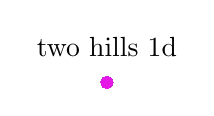
\begin{tikzpicture}

% defining custom colors
\definecolor{mycolor1}{rgb}{1,0.1,0.1}
\definecolor{mycolor2}{rgb}{0.1,1,0.1}
\definecolor{mycolor3}{rgb}{0.1,0.1,1}
\definecolor{mycolor4}{rgb}{0.4,0.4,0.1}
\definecolor{mycolor5}{rgb}{0.1,1,1}
\definecolor{mycolor6}{rgb}{0.9,0.1,0.9}


\begin{axis}[%
view={-72}{42},
xmin=0, xmax=100,
xlabel={Number of samples},
xmajorgrids,
y dir=reverse,
ymin=-40, ymax=40,
ylabel={sample location},
ymajorgrids,
zmin=0, zmax=0.04,
zmajorgrids,
axis lines=left,
scale only axis,
width=\fwidth,
height=\fheight,
title={two hills 1d}]
\addplot3 [
color=mycolor1,
only marks,
mark=*,
mark options={solid}
]
coordinates{
 (1,8.64397318249258,0)(2,0.94202610858281,0)(3,-8.51909224508774,0)(4,8.73504449150106,0)(5,-4.38039043088074,0)(6,-4.29661051911298,0)(7,-11.0272856023819,0)(8,3.9624682112797,0)(9,-9.64925101622627,0)(10,1.68448763331274,0)(11,-19.6535886818246,0)(12,-7.44302088643632,0)(13,-5.52306700484431,0)(14,-8.19726048957947,0)(15,11.0914180018547,0)(16,-6.14945861779946,0)(17,-2.54635294228131,0)(18,-2.6982964643979,0)(19,-16.7199406378983,0)(20,-18.7604530491713,0)(21,5.75006015878006,0)(22,-8.66133150431014,0)(23,-21.1652270104548,0)(24,-9.64465668893709,0)(25,2.12729440847614,0)(26,4.77917410863812,0)(27,1.0065773429252,0)(28,2.97433365310199,0)(29,5.70148492190659,0)(30,-16.2449561946395,0)(31,6.43442896614198,0)(32,6.81861101501212,0)(33,0.146545462976063,0)(34,-13.0154083556885,0)(35,-12.8458694199502,0)(36,8.12213221007246,0)(37,8.38548117504491,0)(38,14.2032099924033,0)(39,-9.89751963936141,0)(40,-11.8322927670026,0)(41,-4.66258701033501,0)(42,-3.65943456601606,0)(43,11.1833282594471,0)(44,-4.65614764979949,0)(45,-15.6079951442098,0)(46,-2.83103049634655,0)(47,-13.2294142478163,0)(48,-1.96238020663121,0)(49,4.19039092209372,0)(50,7.42318242363705,0)(51,-1.43031901660663,0)(52,-21.6194345485188,0)(53,-6.44226188013935,0)(54,14.3958966362552,0)(55,-8.46916703704845,0)(56,0.573396598842837,0)(57,6.43407819310009,0)(58,-6.70431031039433,0)(59,-0.0314182038723435,0)(60,3.5293137585827,0)(61,11.7950226794027,0)(62,-6.85902078686398,0)(63,16.7678943259546,0)(64,-2.55308776295612,0)(65,-6.47548492231093,0)(66,-1.82214217198884,0)(67,8.51800292262651,0)(68,-3.06550037434344,0)(69,-4.40528888444301,0)(70,-6.11471876975789,0)(71,-4.85206910127117,0)(72,11.9701928905678,0)(73,13.9478769033299,0)(74,1.65367561474691,0)(75,-5.09966956368727,0)(76,13.7771664896642,0)(77,12.9851755410422,0)(78,-1.30117041997769,0)(79,7.40248586252175,0)(80,13.320174467912,0)(81,-2.78070689182663,0)(82,-3.27992902252155,0)(83,-0.125272443409905,0)(84,9.03178709204238,0)(85,-11.1246332865596,0)(86,-8.39210796544983,0)(87,0.355343920326862,0)(88,-12.4652893677206,0)(89,8.84505037335452,0)(90,25.3833384421976,0)(91,13.1679503886664,0)(92,14.4221307180034,0)(93,14.6691939938362,0)(94,-11.0705180813558,0)(95,-4.60936138301192,0)(96,-0.202959162388906,0)(97,-0.459981798696434,0)(98,-5.44486576241684,0)(99,9.17034563222667,0)(100,-0.194183076797647,0) 
};

\addplot3 [
color=mycolor2,
only marks,
mark=*,
mark options={solid}
]
coordinates{
 (1,8.94186799433925,0)(2,6.24789448518379,0)(3,9.01015809078886,0)(4,7.6249570105499,0)(5,6.26624946464636,0)(6,6.26624946464636,0)(7,7.51929193501207,0)(8,7.51929193501207,0)(9,8.05197369617755,0)(10,8.05197369617755,0)(11,8.05197369617755,0)(12,8.05197369617755,0)(13,8.05197369617755,0)(14,11.559388032863,0)(15,9.6147584719433,0)(16,8.80953096951528,0)(17,7.9562547065276,0)(18,7.9562547065276,0)(19,7.9562547065276,0)(20,9.77458338500104,0)(21,9.77458338500104,0)(22,9.77458338500104,0)(23,9.77458338500104,0)(24,10.4472929434536,0)(25,10.4472929434536,0)(26,10.4472929434536,0)(27,11.3878598299627,0)(28,11.3878598299627,0)(29,11.3878598299627,0)(30,11.3878598299627,0)(31,11.3878598299627,0)(32,11.4342015743395,0)(33,11.4342015743395,0)(34,11.4342015743395,0)(35,11.4342015743395,0)(36,11.4342015743395,0)(37,11.4342015743395,0)(38,11.4342015743395,0)(39,7.6925020657731,0)(40,7.6925020657731,0)(41,7.6925020657731,0)(42,11.228980977891,0)(43,9.75657780835039,0)(44,9.75657780835039,0)(45,8.86132735896518,0)(46,8.86132735896518,0)(47,8.86132735896518,0)(48,10.1864453189961,0)(49,10.1864453189961,0)(50,9.7341387316832,0)(51,9.7341387316832,0)(52,9.7341387316832,0)(53,9.7341387316832,0)(54,9.7341387316832,0)(55,9.91546265717692,0)(56,9.91546265717692,0)(57,9.91546265717692,0)(58,9.90552734875411,0)(59,9.90552734875411,0)(60,9.90552734875411,0)(61,9.90552734875411,0)(62,9.90552734875411,0)(63,9.90552734875411,0)(64,9.90552734875411,0)(65,9.32931540034101,0)(66,9.32931540034101,0)(67,9.32931540034101,0)(68,9.32931540034101,0)(69,9.32931540034101,0)(70,9.32931540034101,0)(71,9.32931540034101,0)(72,9.32931540034101,0)(73,9.85225354570895,0)(74,9.85225354570895,0)(75,9.85225354570895,0)(76,9.85225354570895,0)(77,9.85225354570895,0)(78,9.85225354570895,0)(79,9.85225354570895,0)(80,9.85225354570895,0)(81,9.85225354570895,0)(82,9.81263892078596,0)(83,9.81263892078596,0)(84,9.81263892078596,0)(85,9.81263892078596,0)(86,9.92500853487859,0)(87,9.92500853487859,0)(88,9.92500853487859,0)(89,9.92500853487859,0)(90,9.92500853487859,0)(91,9.92500853487859,0)(92,9.92500853487859,0)(93,9.92500853487859,0)(94,9.92500853487859,0)(95,9.8608272123637,0)(96,9.71536819575352,0)(97,9.71536819575352,0)(98,9.71536819575352,0)(99,9.65396211517952,0)(100,9.65396211517952,0) 
};

\addplot3 [
color=mycolor3,
only marks,
mark=*,
mark options={solid}
]
coordinates{
 (1,8.94186799433925,0)(2,6.24789448518379,0)(3,9.01015809078886,0)(4,7.6249570105499,0)(5,6.26624946464636,0)(6,6.26624946464636,0)(7,7.51929193501207,0)(8,7.51929193501207,0)(9,8.05197369617755,0)(10,8.05197369617755,0)(11,8.05197369617755,0)(12,8.05197369617755,0)(13,8.05197369617755,0)(14,11.559388032863,0)(15,9.6147584719433,0)(16,8.80953096951528,0)(17,7.9562547065276,0)(18,7.9562547065276,0)(19,7.9562547065276,0)(20,9.77458338500104,0)(21,9.77458338500104,0)(22,9.77458338500104,0)(23,9.77458338500104,0)(24,10.4472929434536,0)(25,10.4472929434536,0)(26,10.4472929434536,0)(27,11.3878598299627,0)(28,11.3878598299627,0)(29,11.3878598299627,0)(30,11.3878598299627,0)(31,11.3878598299627,0)(32,11.4342015743395,0)(33,11.4342015743395,0)(34,11.4342015743395,0)(35,11.4342015743395,0)(36,11.4342015743395,0)(37,11.4342015743395,0)(38,11.4342015743395,0)(39,7.6925020657731,0)(40,7.6925020657731,0)(41,7.6925020657731,0)(42,11.228980977891,0)(43,9.75657780835039,0)(44,9.75657780835039,0)(45,8.86132735896518,0)(46,8.86132735896518,0)(47,8.86132735896518,0)(48,10.1864453189961,0)(49,10.1864453189961,0)(50,9.7341387316832,0)(51,9.7341387316832,0)(52,9.7341387316832,0)(53,9.7341387316832,0)(54,9.7341387316832,0)(55,9.91546265717692,0)(56,9.91546265717692,0)(57,9.91546265717692,0)(58,9.90552734875411,0)(59,9.90552734875411,0)(60,9.90552734875411,0)(61,9.90552734875411,0)(62,9.90552734875411,0)(63,9.90552734875411,0)(64,9.90552734875411,0)(65,9.32931540034101,0)(66,9.32931540034101,0)(67,9.32931540034101,0)(68,9.32931540034101,0)(69,9.32931540034101,0)(70,9.32931540034101,0)(71,9.32931540034101,0)(72,9.32931540034101,0)(73,9.85225354570895,0)(74,9.85225354570895,0)(75,9.85225354570895,0)(76,9.85225354570895,0)(77,9.85225354570895,0)(78,9.85225354570895,0)(79,9.85225354570895,0)(80,9.85225354570895,0)(81,9.85225354570895,0)(82,9.81263892078596,0)(83,9.81263892078596,0)(84,9.81263892078596,0)(85,9.81263892078596,0)(86,9.92500853487859,0)(87,9.92500853487859,0)(88,9.92500853487859,0)(89,9.92500853487859,0)(90,9.92500853487859,0)(91,9.92500853487859,0)(92,9.92500853487859,0)(93,9.92500853487859,0)(94,9.92500853487859,0)(95,9.8608272123637,0)(96,9.71536819575352,0)(97,9.71536819575352,0)(98,9.71536819575352,0)(99,9.65396211517952,0)(100,9.65396211517952,0) 
};

\addplot3 [
color=mycolor4,
only marks,
mark=*,
mark options={solid}
]
coordinates{
 (1,0,0)(2,-13.1063646161906,0)(3,0.678229483890732,0)(4,-3.59945588564868,0)(5,-10.6247125319566,0)(6,0.291067912868716,0)(7,3.89876870194523,0)(8,12.4481439316606,0)(9,-9.05291428473774,0)(10,20.3399513727934,0)(11,-1.05275316545479,0)(12,-8.24561759528231,0)(13,-0.445969698524856,0)(14,-6.26666227973692,0)(15,1.67132333701364,0)(16,-7.71635343541967,0)(17,-1.05275316545479,0)(18,-8.24561759528231,0)(19,-0.445969698524856,0)(20,-6.26666227973692,0)(21,1.67132333701364,0)(22,-7.71635343541967,0)(23,-12.5524049590666,0)(24,6.96179875036652,0)(25,-1.2274694683746,0)(26,-1.05275316545479,0)(27,-8.24561759528231,0)(28,-0.445969698524856,0)(29,-6.26666227973692,0)(30,1.67132333701364,0)(31,-7.71635343541967,0)(32,-12.5524049590666,0)(33,6.96179875036652,0)(34,-1.2274694683746,0)(35,18.9117696246173,0)(36,12.5707786145661,0)(37,-0.848456051344682,0)(38,10.3156128783239,0)(39,3.17562026337821,0)(40,-0.90855847709705,0)(41,-1.05275316545479,0)(42,-8.24561759528231,0)(43,-0.445969698524856,0)(44,-6.26666227973692,0)(45,1.67132333701364,0)(46,-7.71635343541967,0)(47,-12.5524049590666,0)(48,6.96179875036652,0)(49,-1.2274694683746,0)(50,18.9117696246173,0)(51,12.5707786145661,0)(52,-0.848456051344682,0)(53,10.3156128783239,0)(54,3.17562026337821,0)(55,-0.90855847709705,0)(56,8.98032503726006,0)(57,-0.54747013960022,0)(58,-9.37765766906571,0)(59,-4.61807231299709,0)(60,16.0419504632786,0)(61,-13.1063646161906,0)(62,0.678229483890732,0)(63,-3.59945588564868,0)(64,-1.05275316545479,0)(65,-8.24561759528231,0)(66,-0.445969698524856,0)(67,-6.26666227973692,0)(68,1.67132333701364,0)(69,-7.71635343541967,0)(70,-12.5524049590666,0)(71,6.96179875036652,0)(72,-1.2274694683746,0)(73,18.9117696246173,0)(74,12.5707786145661,0)(75,-0.848456051344682,0)(76,10.3156128783239,0)(77,3.17562026337821,0)(78,-0.90855847709705,0)(79,8.98032503726006,0)(80,-0.54747013960022,0)(81,-9.37765766906571,0)(82,-4.61807231299709,0)(83,16.0419504632786,0)(84,-13.1063646161906,0)(85,0.678229483890732,0)(86,-3.59945588564868,0)(87,-10.6247125319566,0)(88,0.291067912868716,0)(89,3.89876870194523,0)(90,12.4481439316606,0)(91,-10.0513498209972,0)(92,20.3399513727934,0)(93,-1.36649296170648,0)(94,3.08762330285705,0)(95,1.89793147403423,0)(96,5.2324265351375,0)(97,12.2617662574878,0)(98,9.16166261649394,0)(99,3.51859513355818,0)(100,1.47822332897649,0) 
};

\addplot3 [
color=mycolor5,
only marks,
mark=*,
mark options={solid}
]
coordinates{
 (1,8.64397318249258,0)(2,0.94202610858281,0)(3,-8.51909224508774,0)(4,8.73504449150106,0)(5,-4.38039043088074,0)(6,-4.29661051911298,0)(7,-11.0272856023819,0)(8,3.9624682112797,0)(9,-9.64925101622627,0)(10,1.68448763331274,0)(11,0,0)(12,-19.6535886818246,0)(13,-7.44302088643632,0)(14,-5.52306700484431,0)(15,-8.19726048957947,0)(16,11.0914180018547,0)(17,-6.14945861779946,0)(18,-2.54635294228131,0)(19,-2.6982964643979,0)(20,-16.7199406378983,0)(21,-18.7604530491713,0)(22,5.75006015878006,0)(23,-8.66133150431014,0)(24,-21.1652270104548,0)(25,-9.61937219373153,0)(26,2.12729440847614,0)(27,4.77917410863812,0)(28,1.0065773429252,0)(29,2.97433365310199,0)(30,5.70148492190659,0)(31,-16.2449561946395,0)(32,6.43442896614198,0)(33,6.81861101501212,0)(34,0.146545462976063,0)(35,-13.0154083556885,0)(36,-12.8458694199502,0)(37,8.12213221007246,0)(38,8.38548117504491,0)(39,14.2032099924033,0)(40,-9.89751963936141,0)(41,-11.8322927670026,0)(42,-4.66258701033501,0)(43,-3.65943456601606,0)(44,11.1833282594471,0)(45,-4.65614764979949,0)(46,-15.6079951442098,0)(47,-2.83103049634655,0)(48,-13.2294142478163,0)(49,-1.96238020663121,0)(50,4.19039092209372,0)(51,7.42318242363705,0)(52,-1.43031901660663,0)(53,-21.6194345485188,0)(54,-6.44226188013935,0)(55,14.3958966362552,0)(56,-8.46916703704845,0)(57,0.573396598842837,0)(58,6.43407819310009,0)(59,-6.70431031039433,0)(60,-0.0314182038723435,0)(61,3.5293137585827,0)(62,11.7950226794027,0)(63,-6.85902078686398,0)(64,16.7678943259546,0)(65,-2.55308776295612,0)(66,-6.47548492231093,0)(67,-1.82214217198884,0)(68,8.51800292262651,0)(69,-3.06550037434344,0)(70,-4.40528888444301,0)(71,-6.11471876975789,0)(72,-4.85206910127117,0)(73,11.9701928905678,0)(74,13.9478769033299,0)(75,1.65367561474691,0)(76,-5.09966956368727,0)(77,13.7771664896642,0)(78,12.9851755410422,0)(79,-1.30117041997769,0)(80,7.40248586252175,0)(81,13.320174467912,0)(82,-2.78070689182663,0)(83,-3.27992902252155,0)(84,-0.125272443409905,0)(85,9.03178709204238,0)(86,-11.1246332865596,0)(87,-8.39210796544983,0)(88,0.355343920326862,0)(89,-12.4652893677206,0)(90,8.84505037335452,0)(91,25.3833384421976,0)(92,13.1679503886664,0)(93,14.4221307180034,0)(94,14.6691939938362,0)(95,-11.0705180813558,0)(96,-4.60936138301192,0)(97,-0.202959162388906,0)(98,-0.459981798696434,0)(99,-5.44486576241684,0)(100,9.86193797775324,0) 
};

\addplot3 [
color=mycolor6,
only marks,
mark=*,
mark options={solid}
]
coordinates{
 (1,8.94186799433925,0)(2,6.24789448518379,0)(3,9.01015809078886,0)(4,7.6249570105499,0)(5,6.26624946464636,0)(6,6.26624946464636,0)(7,7.51929193501207,0)(8,7.51929193501207,0)(9,8.05197369617755,0)(10,8.05197369617755,0)(11,8.05197369617755,0)(12,8.05197369617755,0)(13,8.05197369617755,0)(14,11.559388032863,0)(15,9.6147584719433,0)(16,8.80953096951528,0)(17,7.9562547065276,0)(18,7.9562547065276,0)(19,7.9562547065276,0)(20,9.77458338500104,0)(21,9.77458338500104,0)(22,9.77458338500104,0)(23,9.77458338500104,0)(24,10.4472929434536,0)(25,10.4472929434536,0)(26,10.4472929434536,0)(27,11.3878598299627,0)(28,11.3878598299627,0)(29,11.3878598299627,0)(30,11.3878598299627,0)(31,11.3878598299627,0)(32,11.4342015743395,0)(33,11.4342015743395,0)(34,11.4342015743395,0)(35,11.4342015743395,0)(36,11.4342015743395,0)(37,11.4342015743395,0)(38,11.4342015743395,0)(39,7.6925020657731,0)(40,7.6925020657731,0)(41,7.6925020657731,0)(42,11.228980977891,0)(43,9.75657780835039,0)(44,9.75657780835039,0)(45,8.86132735896518,0)(46,8.86132735896518,0)(47,8.86132735896518,0)(48,10.1864453189961,0)(49,10.1864453189961,0)(50,9.7341387316832,0)(51,9.7341387316832,0)(52,9.7341387316832,0)(53,9.7341387316832,0)(54,9.7341387316832,0)(55,9.91546265717692,0)(56,9.91546265717692,0)(57,9.91546265717692,0)(58,9.90552734875411,0)(59,9.90552734875411,0)(60,9.90552734875411,0)(61,9.90552734875411,0)(62,9.90552734875411,0)(63,9.90552734875411,0)(64,9.90552734875411,0)(65,9.32931540034101,0)(66,9.32931540034101,0)(67,9.32931540034101,0)(68,9.32931540034101,0)(69,9.32931540034101,0)(70,9.32931540034101,0)(71,9.32931540034101,0)(72,9.32931540034101,0)(73,9.85225354570895,0)(74,9.85225354570895,0)(75,9.85225354570895,0)(76,9.85225354570895,0)(77,9.85225354570895,0)(78,9.85225354570895,0)(79,9.85225354570895,0)(80,9.85225354570895,0)(81,9.85225354570895,0)(82,9.81263892078596,0)(83,9.81263892078596,0)(84,9.81263892078596,0)(85,9.81263892078596,0)(86,9.92500853487859,0)(87,9.92500853487859,0)(88,9.92500853487859,0)(89,9.92500853487859,0)(90,9.92500853487859,0)(91,9.92500853487859,0)(92,9.92500853487859,0)(93,9.92500853487859,0)(94,9.92500853487859,0)(95,9.8608272123637,0)(96,9.71536819575352,0)(97,9.71536819575352,0)(98,9.71536819575352,0)(99,9.65396211517952,0)(100,9.65396211517952,0) 
};

\addplot3 [
color=black,
solid,
line width=2.0pt
]
coordinates{
 (101,-40,1.33830225764885e-05)(101,-39.9199199199199,1.38182046410497e-05)(101,-39.8398398398398,1.42666228042307e-05)(101,-39.7597597597598,1.47286481503254e-05)(101,-39.6796796796797,1.52046611333821e-05)(101,-39.5995995995996,1.56950517814782e-05)(101,-39.5195195195195,1.6200219904485e-05)(101,-39.4394394394394,1.6720575305353e-05)(101,-39.3593593593594,1.72565379949497e-05)(101,-39.2792792792793,1.7808538410479e-05)(101,-39.1991991991992,1.83770176375138e-05)(101,-39.1191191191191,1.89624276356684e-05)(101,-39.039039039039,1.95652314679408e-05)(101,-38.958958958959,2.01859035337517e-05)(101,-38.8788788788789,2.08249298057069e-05)(101,-38.7987987987988,2.14828080701089e-05)(101,-38.7187187187187,2.21600481712426e-05)(101,-38.6386386386386,2.285717225946e-05)(101,-38.5585585585586,2.35747150430845e-05)(101,-38.4784784784785,2.43132240441603e-05)(101,-38.3983983983984,2.50732598580649e-05)(101,-38.3183183183183,2.58553964170059e-05)(101,-38.2382382382382,2.66602212574213e-05)(101,-38.1581581581582,2.74883357912987e-05)(101,-38.0780780780781,2.83403555814326e-05)(101,-37.997997997998,2.92169106206323e-05)(101,-37.9179179179179,3.01186456148956e-05)(101,-37.8378378378378,3.104622027056e-05)(101,-37.7577577577578,3.20003095854415e-05)(101,-37.6776776776777,3.29816041439723e-05)(101,-37.5975975975976,3.39908104163431e-05)(101,-37.5175175175175,3.50286510616579e-05)(101,-37.4374374374374,3.60958652351047e-05)(101,-37.3573573573574,3.71932088991451e-05)(101,-37.2772772772773,3.8321455138726e-05)(101,-37.1971971971972,3.94813944805093e-05)(101,-37.1171171171171,4.06738352161196e-05)(101,-37.037037037037,4.18996037294058e-05)(101,-36.956956956957,4.31595448277079e-05)(101,-36.8768768768769,4.4454522077123e-05)(101,-36.7967967967968,4.57854181417587e-05)(101,-36.7167167167167,4.71531351269623e-05)(101,-36.6366366366366,4.85585949265103e-05)(101,-36.5565565565566,5.00027395737409e-05)(101,-36.4764764764765,5.14865315966113e-05)(101,-36.3963963963964,5.30109543766577e-05)(101,-36.3163163163163,5.45770125118335e-05)(101,-36.2362362362362,5.61857321831992e-05)(101,-36.1561561561562,5.78381615254348e-05)(101,-36.0760760760761,5.95353710011453e-05)(101,-35.995995995996,6.12784537789192e-05)(101,-35.9159159159159,6.30685261151104e-05)(101,-35.8358358358358,6.49067277392972e-05)(101,-35.7557557557558,6.67942222433795e-05)(101,-35.6756756756757,6.87321974742665e-05)(101,-35.5955955955956,7.07218659301082e-05)(101,-35.5155155155155,7.27644651600165e-05)(101,-35.4354354354354,7.48612581672246e-05)(101,-35.3553553553554,7.70135338156225e-05)(101,-35.2752752752753,7.9222607239612e-05)(101,-35.1951951951952,8.1489820257214e-05)(101,-35.1151151151151,8.38165417863602e-05)(101,-35.035035035035,8.62041682643007e-05)(101,-34.954954954955,8.86541240700501e-05)(101,-34.8748748748749,9.11678619497959e-05)(101,-34.7947947947948,9.37468634451866e-05)(101,-34.7147147147147,9.63926393244148e-05)(101,-34.6346346346346,9.91067300160058e-05)(101,-34.5545545545546,0.00010189070604522)(101,-34.4744744744745,0.000104746168472971)(101,-34.3943943943944,0.00010767474933716)(101,-34.3143143143143,0.000110678112096323)(101,-34.2342342342342,0.000113757952075483)(101,-34.1541541541542,0.000116915996914087)(101,-34.0740740740741,0.000120154007015926)(101,-33.993993993994,0.000123473776000907)(101,-33.9139139139139,0.000126877131158549)(101,-33.8338338338338,0.000130365933903088)(101,-33.7537537537538,0.000133942080230046)(101,-33.6736736736737,0.000137607501174126)(101,-33.5935935935936,0.0001413641632683)(101,-33.5135135135135,0.000145214069003937)(101,-33.4334334334334,0.00014915925729182)(101,-33.3533533533534,0.000153201803923895)(101,-33.2732732732733,0.000157343822035606)(101,-33.1931931931932,0.000161587462568624)(101,-33.1131131131131,0.000165934914733831)(101,-33.033033033033,0.000170388406474362)(101,-32.952952952953,0.000174950204928538)(101,-32.8728728728729,0.000179622616892505)(101,-32.7927927927928,0.000184407989282385)(101,-32.7127127127127,0.000189308709595757)(101,-32.6326326326326,0.000194327206372254)(101,-32.5525525525526,0.000199465949653091)(101,-32.4724724724725,0.000204727451439301)(101,-32.3923923923924,0.000210114266148476)(101,-32.3123123123123,0.000215628991069791)(101,-32.2322322322322,0.000221274266817093)(101,-32.1521521521522,0.000227052777779814)(101,-32.0720720720721,0.000232967252571501)(101,-31.991991991992,0.000239020464475689)(101,-31.9119119119119,0.000245215231888918)(101,-31.8318318318318,0.000251554418760605)(101,-31.7517517517518,0.000258040935029545)(101,-31.6716716716717,0.000264677737056775)(101,-31.5915915915916,0.000271467828054534)(101,-31.5115115115115,0.000278414258511061)(101,-31.4314314314314,0.000285520126610952)(101,-31.3513513513514,0.000292788578650791)(101,-31.2712712712713,0.000300222809449793)(101,-31.1911911911912,0.000307826062755151)(101,-31.1111111111111,0.000315601631641804)(101,-31.031031031031,0.000323552858906328)(101,-30.950950950951,0.000331683137454643)(101,-30.8708708708709,0.000339995910683238)(101,-30.7907907907908,0.000348494672853595)(101,-30.7107107107107,0.000357182969459489)(101,-30.6306306306306,0.000366064397586863)(101,-30.5505505505506,0.000375142606265932)(101,-30.4704704704705,0.000384421296815189)(101,-30.3903903903904,0.000393904223176991)(101,-30.3103103103103,0.000403595192244368)(101,-30.2302302302302,0.000413498064178719)(101,-30.1501501501502,0.000423616752718052)(101,-30.0700700700701,0.000433955225475398)(101,-29.98998998999,0.000444517504227068)(101,-29.9099099099099,0.000455307665190355)(101,-29.8298298298298,0.000466329839290368)(101,-29.7497497497497,0.000477588212415564)(101,-29.6696696696697,0.000489087025661667)(101,-29.5895895895896,0.000500830575563558)(101,-29.5095095095095,0.000512823214314763)(101,-29.4294294294294,0.000525069349974172)(101,-29.3493493493493,0.000537573446659573)(101,-29.2692692692693,0.000550340024727644)(101,-29.1891891891892,0.000563373660939975)(101,-29.1091091091091,0.00057667898861475)(101,-29.029029029029,0.000590260697763673)(101,-28.9489489489489,0.000604123535213746)(101,-28.8688688688689,0.000618272304713484)(101,-28.7887887887888,0.000632711867023164)(101,-28.7087087087087,0.000647447139988702)(101,-28.6286286286286,0.000662483098598742)(101,-28.5485485485485,0.000677824775024529)(101,-28.4684684684685,0.00069347725864219)(101,-28.3883883883884,0.000709445696036946)(101,-28.3083083083083,0.000725735290988892)(101,-28.2282282282282,0.000742351304439893)(101,-28.1481481481481,0.000759299054441176)(101,-28.0680680680681,0.00077658391608121)(101,-27.987987987988,0.000794211321393438)(101,-27.9079079079079,0.000812186759243431)(101,-27.8278278278278,0.000830515775195072)(101,-27.7477477477477,0.000849203971355292)(101,-27.6676676676677,0.000868257006197)(101,-27.5875875875876,0.000887680594359711)(101,-27.5075075075075,0.00090748050642751)(101,-27.4274274274274,0.000927662568683897)(101,-27.3473473473473,0.0009482326628431)(101,-27.2672672672673,0.000969196725757424)(101,-27.1871871871872,0.000990560749100247)(101,-27.1071071071071,0.00101233077902421)(101,-27.027027027027,0.00103451291579421)(101,-26.9469469469469,0.00105711331339476)(101,-26.8668668668669,0.00108013817911136)(101,-26.7867867867868,0.0011035937730854)(101,-26.7067067067067,0.00112748640784219)(101,-26.6266266266266,0.00115182244779185)(101,-26.5465465465465,0.00117660830870247)(101,-26.4664664664665,0.00120185045714527)(101,-26.3863863863864,0.00122755540991133)(101,-26.3063063063063,0.00125372973339956)(101,-26.2262262262262,0.00128038004297541)(101,-26.1461461461461,0.00130751300230007)(101,-26.0660660660661,0.00133513532262973)(101,-25.985985985986,0.00136325376208454)(101,-25.9059059059059,0.00139187512488693)(101,-25.8258258258258,0.0014210062605689)(101,-25.7457457457457,0.00145065406314803)(101,-25.6656656656657,0.00148082547027168)(101,-25.5855855855856,0.00151152746232934)(101,-25.5055055055055,0.00154276706153247)(101,-25.4254254254254,0.00157455133096184)(101,-25.3453453453453,0.00160688737358179)(101,-25.2652652652653,0.0016397823312213)(101,-25.1851851851852,0.00167324338352152)(101,-25.1051051051051,0.00170727774684939)(101,-25.025025025025,0.00174189267317727)(101,-24.9449449449449,0.00177709544892815)(101,-24.8648648648649,0.00181289339378627)(101,-24.7847847847848,0.00184929385947285)(101,-24.7047047047047,0.00188630422848682)(101,-24.6246246246246,0.00192393191281025)(101,-24.5445445445445,0.00196218435257817)(101,-24.4644644644645,0.00200106901471285)(101,-24.3843843843844,0.0020405933915221)(101,-24.3043043043043,0.0020807649992616)(101,-24.2242242242242,0.00212159137666093)(101,-24.1441441441441,0.00216308008341344)(101,-24.0640640640641,0.00220523869862944)(101,-23.983983983984,0.00224807481925294)(101,-23.9039039039039,0.0022915960584417)(101,-23.8238238238238,0.00233581004391047)(101,-23.7437437437437,0.0023807244162374)(101,-23.6636636636637,0.00242634682713357)(101,-23.5835835835836,0.00247268493767558)(101,-23.5035035035035,0.00251974641650119)(101,-23.4234234234234,0.00256753893796796)(101,-23.3433433433433,0.00261607018027502)(101,-23.2632632632633,0.00266534782354776)(101,-23.1831831831832,0.00271537954788581)(101,-23.1031031031031,0.00276617303137407)(101,-23.023023023023,0.00281773594805703)(101,-22.9429429429429,0.00287007596587648)(101,-22.8628628628629,0.00292320074457259)(101,-22.7827827827828,0.0029771179335487)(101,-22.7027027027027,0.00303183516969979)(101,-22.6226226226226,0.00308736007520491)(101,-22.5425425425425,0.00314370025528369)(101,-22.4624624624625,0.00320086329591723)(101,-22.3823823823824,0.00325885676153351)(101,-22.3023023023023,0.00331768819265761)(101,-22.2222222222222,0.00337736510352706)(101,-22.1421421421421,0.00343789497967251)(101,-22.0620620620621,0.00349928527546413)(101,-21.981981981982,0.00356154341162401)(101,-21.9019019019019,0.00362467677270497)(101,-21.8218218218218,0.00368869270453615)(101,-21.7417417417417,0.00375359851163568)(101,-21.6616616616617,0.00381940145459099)(101,-21.5815815815816,0.00388610874740723)(101,-21.5015015015015,0.00395372755482399)(101,-21.4214214214214,0.0040222649896012)(101,-21.3413413413413,0.00409172810977437)(101,-21.2612612612613,0.00416212391588003)(101,-21.1811811811812,0.00423345934815158)(101,-21.1011011011011,0.00430574128368641)(101,-21.021021021021,0.00437897653358481)(101,-20.9409409409409,0.00445317184006117)(101,-20.8608608608609,0.00452833387352837)(101,-20.7807807807808,0.00460446922965576)(101,-20.7007007007007,0.00468158442640166)(101,-20.6206206206206,0.00475968590102091)(101,-20.5405405405405,0.00483878000704834)(101,-20.4604604604605,0.00491887301125894)(101,-20.3803803803804,0.00499997109060533)(101,-20.3003003003003,0.00508208032913362)(101,-20.2202202202202,0.00516520671487824)(101,-20.1401401401401,0.00524935613673682)(101,-20.0600600600601,0.0053345343813258)(101,-19.97997997998,0.00542074712981784)(101,-19.8998998998999,0.00550799995476186)(101,-19.8198198198198,0.00559629831688667)(101,-19.7397397397397,0.00568564756188931)(101,-19.6596596596597,0.00577605291720876)(101,-19.5795795795796,0.0058675194887865)(101,-19.4994994994995,0.00596005225781458)(101,-19.4194194194194,0.00605365607747232)(101,-19.3393393393393,0.0061483356696531)(101,-19.2592592592593,0.0062440956216817)(101,-19.1791791791792,0.00634094038302401)(101,-19.0990990990991,0.00643887426198963)(101,-19.019019019019,0.00653790142242912)(101,-18.9389389389389,0.00663802588042656)(101,-18.8588588588589,0.00673925150098903)(101,-18.7787787787788,0.00684158199473404)(101,-18.6986986986987,0.00694502091457626)(101,-18.6186186186186,0.00704957165241465)(101,-18.5385385385385,0.00715523743582165)(101,-18.4584584584585,0.00726202132473521)(101,-18.3783783783784,0.00736992620815557)(101,-18.2982982982983,0.00747895480084762)(101,-18.2182182182182,0.00758910964005057)(101,-18.1381381381381,0.00770039308219614)(101,-18.0580580580581,0.00781280729963669)(101,-17.977977977978,0.00792635427738473)(101,-17.8978978978979,0.00804103580986525)(101,-17.8178178178178,0.00815685349768226)(101,-17.7377377377377,0.00827380874440108)(101,-17.6576576576577,0.00839190275334777)(101,-17.5775775775776,0.00851113652442723)(101,-17.4974974974975,0.0086315108509615)(101,-17.4174174174174,0.00875302631654975)(101,-17.3373373373373,0.00887568329195139)(101,-17.2572572572573,0.00899948193199405)(101,-17.1771771771772,0.00912442217250772)(101,-17.0970970970971,0.00925050372728685)(101,-17.017017017017,0.00937772608508176)(101,-16.9369369369369,0.00950608850662112)(101,-16.8568568568569,0.00963559002166691)(101,-16.7767767767768,0.00976622942610364)(101,-16.6966966966967,0.0098980052790632)(101,-16.6166166166166,0.0100309159000872)(101,-16.5365365365365,0.0101649593663279)(101,-16.4564564564565,0.0103001335097907)(101,-16.3763763763764,0.010436435914617)(101,-16.2962962962963,0.0105738639144131)(101,-16.2162162162162,0.0107124145896225)(101,-16.1361361361361,0.0108520847649465)(101,-16.0560560560561,0.010992871006813)(101,-15.975975975976,0.0111347696208955)(101,-15.8958958958959,0.0112777766496842)(101,-15.8158158158158,0.0114218878701105)(101,-15.7357357357357,0.0115670987912262)(101,-15.6556556556557,0.0117134046519405)(101,-15.5755755755756,0.011860800418814)(101,-15.4954954954955,0.0120092807839133)(101,-15.4154154154154,0.0121588401627275)(101,-15.3353353353353,0.0123094726921466)(101,-15.2552552552553,0.0124611722285057)(101,-15.1751751751752,0.012613932345695)(101,-15.0950950950951,0.0127677463333369)(101,-15.015015015015,0.0129226071950339)(101,-14.9349349349349,0.0130785076466857)(101,-14.8548548548549,0.0132354401148798)(101,-14.7747747747748,0.0133933967353555)(101,-14.6946946946947,0.013552369351543)(101,-14.6146146146146,0.0137123495131801)(101,-14.5345345345345,0.013873328475006)(101,-14.4544544544545,0.0140352971955359)(101,-14.3743743743744,0.0141982463359159)(101,-14.2942942942943,0.0143621662588612)(101,-14.2142142142142,0.014527047027677)(101,-14.1341341341341,0.0146928784053658)(101,-14.0540540540541,0.0148596498538208)(101,-13.973973973974,0.0150273505331067)(101,-13.8938938938939,0.0151959693008306)(101,-13.8138138138138,0.0153654947116025)(101,-13.7337337337337,0.0155359150165875)(101,-13.6536536536537,0.0157072181631514)(101,-13.5735735735736,0.0158793917945997)(101,-13.4934934934935,0.0160524232500122)(101,-13.4134134134134,0.016226299564173)(101,-13.3333333333333,0.0164010074675994)(101,-13.2532532532533,0.0165765333866673)(101,-13.1731731731732,0.0167528634438376)(101,-13.0930930930931,0.0169299834579821)(101,-13.013013013013,0.017107878944811)(101,-12.9329329329329,0.0172865351174024)(101,-12.8528528528529,0.0174659368868355)(101,-12.7727727727728,0.0176460688629273)(101,-12.6926926926927,0.0178269153550739)(101,-12.6126126126126,0.018008460373198)(101,-12.5325325325325,0.0181906876288021)(101,-12.4524524524525,0.0183735805361283)(101,-12.3723723723724,0.0185571222134271)(101,-12.2922922922923,0.0187412954843324)(101,-12.2122122122122,0.018926082879347)(101,-12.1321321321321,0.0191114666374361)(101,-12.0520520520521,0.0192974287077311)(101,-11.971971971972,0.0194839507513435)(101,-11.8918918918919,0.019671014143289)(101,-11.8118118118118,0.0198585999745227)(101,-11.7317317317317,0.0200466890540856)(101,-11.6516516516517,0.0202352619113618)(101,-11.5715715715716,0.0204242987984477)(101,-11.4914914914915,0.0206137796926331)(101,-11.4114114114114,0.0208036842989938)(101,-11.3313313313313,0.0209939920530956)(101,-11.2512512512513,0.021184682123811)(101,-11.1711711711712,0.021375733416247)(101,-11.0910910910911,0.0215671245747847)(101,-11.011011011011,0.0217588339862305)(101,-10.9309309309309,0.0219508397830784)(101,-10.8508508508509,0.0221431198468836)(101,-10.7707707707708,0.0223356518117463)(101,-10.6906906906907,0.0225284130679063)(101,-10.6106106106106,0.022721380765447)(101,-10.5305305305305,0.0229145318181096)(101,-10.4504504504505,0.0231078429072154)(101,-10.3703703703704,0.0233012904856966)(101,-10.2902902902903,0.0234948507822352)(101,-10.2102102102102,0.0236884998055083)(101,-10.1301301301301,0.0238822133485401)(101,-10.0500500500501,0.024075966993159)(101,-9.96996996996997,0.0242697361145593)(101,-9.88988988988989,0.0244634958859672)(101,-9.80980980980981,0.0246572212834085)(101,-9.72972972972973,0.0248508870905785)(101,-9.64964964964965,0.025044467903813)(101,-9.56956956956957,0.0252379381371581)(101,-9.48948948948949,0.0254312720275384)(101,-9.40940940940941,0.0256244436400228)(101,-9.32932932932933,0.0258174268731856)(101,-9.24924924924925,0.0260101954645623)(101,-9.16916916916917,0.0262027229961987)(101,-9.08908908908909,0.0263949829002911)(101,-9.00900900900901,0.0265869484649171)(101,-8.92892892892893,0.0267785928398552)(101,-8.84884884884885,0.0269698890424904)(101,-8.76876876876877,0.0271608099638066)(101,-8.68868868868869,0.0273513283744617)(101,-8.60860860860861,0.0275414169309444)(101,-8.52852852852853,0.0277310481818124)(101,-8.44844844844845,0.0279201945740075)(101,-8.36836836836837,0.0281088284592474)(101,-8.28828828828829,0.028296922100493)(101,-8.20820820820821,0.0284844476784867)(101,-8.12812812812813,0.0286713772983616)(101,-8.04804804804805,0.0288576829963198)(101,-7.96796796796797,0.0290433367463758)(101,-7.88788788788789,0.0292283104671645)(101,-7.80780780780781,0.0294125760288111)(101,-7.72772772772772,0.0295961052598603)(101,-7.64764764764764,0.029778869954263)(101,-7.56756756756756,0.0299608418784177)(101,-7.48748748748748,0.0301419927782648)(101,-7.4074074074074,0.0303222943864308)(101,-7.32732732732732,0.0305017184294204)(101,-7.24724724724724,0.0306802366348536)(101,-7.16716716716716,0.0308578207387456)(101,-7.08708708708708,0.0310344424928268)(101,-7.007007007007,0.0312100736719007)(101,-6.92692692692692,0.0313846860812361)(101,-6.84684684684684,0.031558251563992)(101,-6.76676676676676,0.0317307420086723)(101,-6.68668668668668,0.0319021293566066)(101,-6.6066066066066,0.032072385609456)(101,-6.52652652652652,0.0322414828367396)(101,-6.44644644644644,0.0324093931833804)(101,-6.36636636636636,0.0325760888772662)(101,-6.28628628628628,0.0327415422368237)(101,-6.2062062062062,0.0329057256786028)(101,-6.12612612612612,0.0330686117248681)(101,-6.04604604604604,0.033230173011195)(101,-5.96596596596596,0.0333903822940662)(101,-5.88588588588588,0.0335492124584683)(101,-5.8058058058058,0.0337066365254824)(101,-5.72572572572572,0.0338626276598684)(101,-5.64564564564564,0.0340171591776383)(101,-5.56556556556556,0.0341702045536168)(101,-5.48548548548548,0.0343217374289848)(101,-5.4054054054054,0.0344717316188045)(101,-5.32532532532532,0.0346201611195215)(101,-5.24524524524524,0.0347670001164422)(101,-5.16516516516516,0.0349122229911825)(101,-5.08508508508508,0.0350558043290856)(101,-5.005005005005,0.0351977189266053)(101,-4.92492492492492,0.0353379417986526)(101,-4.84484484484484,0.0354764481859011)(101,-4.76476476476476,0.0356132135620502)(101,-4.68468468468468,0.0357482136410418)(101,-4.6046046046046,0.0358814243842273)(101,-4.52452452452452,0.0360128220074839)(101,-4.44444444444444,0.0361423829882743)(101,-4.36436436436436,0.0362700840726495)(101,-4.28428428428428,0.0363959022821904)(101,-4.2042042042042,0.0365198149208855)(101,-4.12412412412412,0.0366417995819425)(101,-4.04404404404404,0.03676183415453)(101,-3.96396396396396,0.0368798968304465)(101,-3.88388388388388,0.0369959661107154)(101,-3.8038038038038,0.037110020812101)(101,-3.72372372372372,0.0372220400735444)(101,-3.64364364364364,0.0373320033625156)(101,-3.56356356356356,0.0374398904812801)(101,-3.48348348348348,0.0375456815730761)(101,-3.4034034034034,0.0376493571282005)(101,-3.32332332332332,0.0377508979900006)(101,-3.24324324324324,0.0378502853607702)(101,-3.16316316316316,0.0379475008075448)(101,-3.08308308308308,0.0380425262677969)(101,-3.003003003003,0.0381353440550259)(101,-2.92292292292292,0.0382259368642425)(101,-2.84284284284284,0.038314287777343)(101,-2.76276276276276,0.0384003802683735)(101,-2.68268268268268,0.03848419820868)(101,-2.6026026026026,0.0385657258719425)(101,-2.52252252252252,0.0386449479390916)(101,-2.44244244244244,0.0387218495031049)(101,-2.36236236236236,0.0387964160736804)(101,-2.28228228228228,0.038868633581787)(101,-2.2022022022022,0.0389384883840873)(101,-2.12212212212212,0.0390059672672329)(101,-2.04204204204204,0.0390710574520297)(101,-1.96196196196196,0.0391337465974705)(101,-1.88188188188188,0.039194022804635)(101,-1.8018018018018,0.0392518746204527)(101,-1.72172172172172,0.0393072910413305)(101,-1.64164164164164,0.0393602615166401)(101,-1.56156156156156,0.0394107759520657)(101,-1.48148148148148,0.0394588247128102)(101,-1.4014014014014,0.0395043986266573)(101,-1.32132132132132,0.03954748898689)(101,-1.24124124124124,0.0395880875550626)(101,-1.16116116116116,0.0396261865636259)(101,-1.08108108108108,0.0396617787184037)(101,-1.001001001001,0.0396948572009207)(101,-0.920920920920921,0.0397254156705792)(101,-0.840840840840841,0.0397534482666846)(101,-0.76076076076076,0.039778949610319)(101,-0.68068068068068,0.039801914806061)(101,-0.6006006006006,0.0398223394435522)(101,-0.52052052052052,0.0398402195989086)(101,-0.44044044044044,0.0398555518359772)(101,-0.36036036036036,0.0398683332074364)(101,-0.28028028028028,0.0398785612557403)(101,-0.2002002002002,0.0398862340139061)(101,-0.12012012012012,0.0398913500061449)(101,-0.04004004004004,0.0398939082483343)(101,0.04004004004004,0.0398939082483343)(101,0.12012012012012,0.0398913500061449)(101,0.2002002002002,0.0398862340139061)(101,0.28028028028028,0.0398785612557403)(101,0.36036036036036,0.0398683332074364)(101,0.44044044044044,0.0398555518359772)(101,0.52052052052052,0.0398402195989086)(101,0.6006006006006,0.0398223394435522)(101,0.68068068068068,0.039801914806061)(101,0.76076076076076,0.039778949610319)(101,0.840840840840841,0.0397534482666846)(101,0.920920920920921,0.0397254156705792)(101,1.001001001001,0.0396948572009207)(101,1.08108108108108,0.0396617787184037)(101,1.16116116116116,0.0396261865636259)(101,1.24124124124124,0.0395880875550626)(101,1.32132132132132,0.03954748898689)(101,1.4014014014014,0.0395043986266573)(101,1.48148148148148,0.0394588247128102)(101,1.56156156156156,0.0394107759520657)(101,1.64164164164164,0.0393602615166401)(101,1.72172172172172,0.0393072910413305)(101,1.8018018018018,0.0392518746204527)(101,1.88188188188188,0.039194022804635)(101,1.96196196196196,0.0391337465974705)(101,2.04204204204204,0.0390710574520297)(101,2.12212212212212,0.0390059672672329)(101,2.2022022022022,0.0389384883840873)(101,2.28228228228228,0.038868633581787)(101,2.36236236236236,0.0387964160736804)(101,2.44244244244244,0.0387218495031049)(101,2.52252252252252,0.0386449479390916)(101,2.6026026026026,0.0385657258719425)(101,2.68268268268268,0.03848419820868)(101,2.76276276276276,0.0384003802683735)(101,2.84284284284284,0.038314287777343)(101,2.92292292292292,0.0382259368642425)(101,3.003003003003,0.0381353440550259)(101,3.08308308308308,0.0380425262677969)(101,3.16316316316316,0.0379475008075448)(101,3.24324324324324,0.0378502853607702)(101,3.32332332332332,0.0377508979900006)(101,3.4034034034034,0.0376493571282005)(101,3.48348348348348,0.0375456815730761)(101,3.56356356356356,0.0374398904812801)(101,3.64364364364364,0.0373320033625156)(101,3.72372372372372,0.0372220400735444)(101,3.8038038038038,0.037110020812101)(101,3.88388388388388,0.0369959661107154)(101,3.96396396396396,0.0368798968304465)(101,4.04404404404404,0.03676183415453)(101,4.12412412412412,0.0366417995819425)(101,4.2042042042042,0.0365198149208855)(101,4.28428428428428,0.0363959022821904)(101,4.36436436436436,0.0362700840726495)(101,4.44444444444444,0.0361423829882743)(101,4.52452452452452,0.0360128220074839)(101,4.6046046046046,0.0358814243842273)(101,4.68468468468468,0.0357482136410418)(101,4.76476476476476,0.0356132135620502)(101,4.84484484484484,0.0354764481859011)(101,4.92492492492492,0.0353379417986526)(101,5.005005005005,0.0351977189266053)(101,5.08508508508508,0.0350558043290856)(101,5.16516516516516,0.0349122229911825)(101,5.24524524524524,0.0347670001164422)(101,5.32532532532532,0.0346201611195215)(101,5.4054054054054,0.0344717316188045)(101,5.48548548548548,0.0343217374289848)(101,5.56556556556556,0.0341702045536168)(101,5.64564564564564,0.0340171591776383)(101,5.72572572572572,0.0338626276598684)(101,5.8058058058058,0.0337066365254824)(101,5.88588588588588,0.0335492124584683)(101,5.96596596596596,0.0333903822940662)(101,6.04604604604604,0.033230173011195)(101,6.12612612612612,0.0330686117248681)(101,6.2062062062062,0.0329057256786028)(101,6.28628628628628,0.0327415422368237)(101,6.36636636636636,0.0325760888772662)(101,6.44644644644644,0.0324093931833804)(101,6.52652652652652,0.0322414828367396)(101,6.6066066066066,0.032072385609456)(101,6.68668668668668,0.0319021293566066)(101,6.76676676676676,0.0317307420086723)(101,6.84684684684684,0.031558251563992)(101,6.92692692692692,0.0313846860812361)(101,7.007007007007,0.0312100736719007)(101,7.08708708708708,0.0310344424928268)(101,7.16716716716716,0.0308578207387456)(101,7.24724724724724,0.0306802366348536)(101,7.32732732732732,0.0305017184294204)(101,7.4074074074074,0.0303222943864308)(101,7.48748748748748,0.0301419927782648)(101,7.56756756756756,0.0299608418784177)(101,7.64764764764764,0.029778869954263)(101,7.72772772772772,0.0295961052598603)(101,7.80780780780781,0.0294125760288111)(101,7.88788788788789,0.0292283104671645)(101,7.96796796796797,0.0290433367463758)(101,8.04804804804805,0.0288576829963198)(101,8.12812812812813,0.0286713772983616)(101,8.20820820820821,0.0284844476784867)(101,8.28828828828829,0.028296922100493)(101,8.36836836836837,0.0281088284592474)(101,8.44844844844845,0.0279201945740075)(101,8.52852852852853,0.0277310481818125)(101,8.60860860860861,0.0275414169309444)(101,8.68868868868869,0.0273513283744617)(101,8.76876876876877,0.0271608099638066)(101,8.84884884884885,0.0269698890424904)(101,8.92892892892893,0.0267785928398552)(101,9.00900900900901,0.0265869484649172)(101,9.08908908908909,0.0263949829002911)(101,9.16916916916917,0.0262027229961987)(101,9.24924924924925,0.0260101954645624)(101,9.32932932932933,0.0258174268731856)(101,9.40940940940941,0.0256244436400228)(101,9.48948948948949,0.0254312720275385)(101,9.56956956956957,0.0252379381371581)(101,9.64964964964965,0.0250444679038131)(101,9.72972972972973,0.0248508870905785)(101,9.80980980980981,0.0246572212834085)(101,9.88988988988989,0.0244634958859673)(101,9.96996996996997,0.0242697361145594)(101,10.0500500500501,0.024075966993159)(101,10.1301301301301,0.0238822133485401)(101,10.2102102102102,0.0236884998055083)(101,10.2902902902903,0.0234948507822352)(101,10.3703703703704,0.0233012904856966)(101,10.4504504504505,0.0231078429072154)(101,10.5305305305305,0.0229145318181096)(101,10.6106106106106,0.022721380765447)(101,10.6906906906907,0.0225284130679062)(101,10.7707707707708,0.0223356518117463)(101,10.8508508508509,0.0221431198468836)(101,10.9309309309309,0.0219508397830784)(101,11.011011011011,0.0217588339862305)(101,11.0910910910911,0.0215671245747847)(101,11.1711711711712,0.021375733416247)(101,11.2512512512513,0.021184682123811)(101,11.3313313313313,0.0209939920530956)(101,11.4114114114114,0.0208036842989938)(101,11.4914914914915,0.0206137796926331)(101,11.5715715715716,0.0204242987984477)(101,11.6516516516517,0.0202352619113618)(101,11.7317317317317,0.0200466890540856)(101,11.8118118118118,0.0198585999745227)(101,11.8918918918919,0.019671014143289)(101,11.971971971972,0.0194839507513435)(101,12.0520520520521,0.0192974287077311)(101,12.1321321321321,0.0191114666374361)(101,12.2122122122122,0.018926082879347)(101,12.2922922922923,0.0187412954843324)(101,12.3723723723724,0.0185571222134271)(101,12.4524524524525,0.0183735805361283)(101,12.5325325325325,0.018190687628802)(101,12.6126126126126,0.018008460373198)(101,12.6926926926927,0.0178269153550739)(101,12.7727727727728,0.0176460688629273)(101,12.8528528528529,0.0174659368868355)(101,12.9329329329329,0.0172865351174024)(101,13.013013013013,0.017107878944811)(101,13.0930930930931,0.0169299834579821)(101,13.1731731731732,0.0167528634438376)(101,13.2532532532533,0.0165765333866673)(101,13.3333333333333,0.0164010074675993)(101,13.4134134134134,0.016226299564173)(101,13.4934934934935,0.0160524232500122)(101,13.5735735735736,0.0158793917945997)(101,13.6536536536537,0.0157072181631514)(101,13.7337337337337,0.0155359150165875)(101,13.8138138138138,0.0153654947116025)(101,13.8938938938939,0.0151959693008306)(101,13.973973973974,0.0150273505331067)(101,14.0540540540541,0.0148596498538208)(101,14.1341341341341,0.0146928784053658)(101,14.2142142142142,0.014527047027677)(101,14.2942942942943,0.0143621662588612)(101,14.3743743743744,0.0141982463359159)(101,14.4544544544545,0.0140352971955359)(101,14.5345345345345,0.013873328475006)(101,14.6146146146146,0.0137123495131801)(101,14.6946946946947,0.013552369351543)(101,14.7747747747748,0.0133933967353555)(101,14.8548548548549,0.0132354401148798)(101,14.9349349349349,0.0130785076466857)(101,15.015015015015,0.0129226071950339)(101,15.0950950950951,0.0127677463333369)(101,15.1751751751752,0.012613932345695)(101,15.2552552552553,0.0124611722285057)(101,15.3353353353353,0.0123094726921466)(101,15.4154154154154,0.0121588401627275)(101,15.4954954954955,0.0120092807839133)(101,15.5755755755756,0.011860800418814)(101,15.6556556556557,0.0117134046519405)(101,15.7357357357357,0.0115670987912262)(101,15.8158158158158,0.0114218878701105)(101,15.8958958958959,0.0112777766496842)(101,15.975975975976,0.0111347696208955)(101,16.0560560560561,0.010992871006813)(101,16.1361361361361,0.0108520847649465)(101,16.2162162162162,0.0107124145896225)(101,16.2962962962963,0.0105738639144131)(101,16.3763763763764,0.010436435914617)(101,16.4564564564565,0.0103001335097907)(101,16.5365365365365,0.0101649593663279)(101,16.6166166166166,0.0100309159000872)(101,16.6966966966967,0.0098980052790632)(101,16.7767767767768,0.00976622942610364)(101,16.8568568568569,0.00963559002166691)(101,16.9369369369369,0.00950608850662112)(101,17.017017017017,0.00937772608508176)(101,17.0970970970971,0.00925050372728685)(101,17.1771771771772,0.00912442217250772)(101,17.2572572572573,0.00899948193199405)(101,17.3373373373373,0.00887568329195139)(101,17.4174174174174,0.00875302631654975)(101,17.4974974974975,0.0086315108509615)(101,17.5775775775776,0.00851113652442723)(101,17.6576576576577,0.00839190275334777)(101,17.7377377377377,0.00827380874440108)(101,17.8178178178178,0.00815685349768226)(101,17.8978978978979,0.00804103580986525)(101,17.977977977978,0.00792635427738473)(101,18.0580580580581,0.00781280729963669)(101,18.1381381381381,0.00770039308219614)(101,18.2182182182182,0.00758910964005057)(101,18.2982982982983,0.00747895480084762)(101,18.3783783783784,0.00736992620815557)(101,18.4584584584585,0.00726202132473521)(101,18.5385385385385,0.00715523743582165)(101,18.6186186186186,0.00704957165241465)(101,18.6986986986987,0.00694502091457626)(101,18.7787787787788,0.00684158199473404)(101,18.8588588588589,0.00673925150098903)(101,18.9389389389389,0.00663802588042656)(101,19.019019019019,0.00653790142242912)(101,19.0990990990991,0.00643887426198963)(101,19.1791791791792,0.00634094038302401)(101,19.2592592592593,0.0062440956216817)(101,19.3393393393393,0.0061483356696531)(101,19.4194194194194,0.00605365607747232)(101,19.4994994994995,0.00596005225781458)(101,19.5795795795796,0.0058675194887865)(101,19.6596596596597,0.00577605291720876)(101,19.7397397397397,0.00568564756188931)(101,19.8198198198198,0.00559629831688667)(101,19.8998998998999,0.00550799995476186)(101,19.97997997998,0.00542074712981784)(101,20.0600600600601,0.0053345343813258)(101,20.1401401401401,0.00524935613673682)(101,20.2202202202202,0.00516520671487824)(101,20.3003003003003,0.00508208032913362)(101,20.3803803803804,0.00499997109060533)(101,20.4604604604605,0.00491887301125894)(101,20.5405405405405,0.00483878000704834)(101,20.6206206206206,0.00475968590102091)(101,20.7007007007007,0.00468158442640166)(101,20.7807807807808,0.00460446922965576)(101,20.8608608608609,0.00452833387352837)(101,20.9409409409409,0.00445317184006117)(101,21.021021021021,0.00437897653358481)(101,21.1011011011011,0.00430574128368641)(101,21.1811811811812,0.00423345934815158)(101,21.2612612612613,0.00416212391588003)(101,21.3413413413413,0.00409172810977437)(101,21.4214214214214,0.0040222649896012)(101,21.5015015015015,0.00395372755482399)(101,21.5815815815816,0.00388610874740723)(101,21.6616616616617,0.00381940145459099)(101,21.7417417417417,0.00375359851163568)(101,21.8218218218218,0.00368869270453615)(101,21.9019019019019,0.00362467677270497)(101,21.981981981982,0.00356154341162401)(101,22.0620620620621,0.00349928527546413)(101,22.1421421421421,0.00343789497967251)(101,22.2222222222222,0.00337736510352706)(101,22.3023023023023,0.00331768819265761)(101,22.3823823823824,0.00325885676153351)(101,22.4624624624625,0.00320086329591723)(101,22.5425425425425,0.00314370025528369)(101,22.6226226226226,0.00308736007520491)(101,22.7027027027027,0.00303183516969979)(101,22.7827827827828,0.0029771179335487)(101,22.8628628628629,0.00292320074457259)(101,22.9429429429429,0.00287007596587648)(101,23.023023023023,0.00281773594805703)(101,23.1031031031031,0.00276617303137407)(101,23.1831831831832,0.00271537954788581)(101,23.2632632632633,0.00266534782354776)(101,23.3433433433433,0.00261607018027502)(101,23.4234234234234,0.00256753893796796)(101,23.5035035035035,0.00251974641650119)(101,23.5835835835836,0.00247268493767558)(101,23.6636636636637,0.00242634682713357)(101,23.7437437437437,0.0023807244162374)(101,23.8238238238238,0.00233581004391047)(101,23.9039039039039,0.0022915960584417)(101,23.983983983984,0.00224807481925294)(101,24.0640640640641,0.00220523869862944)(101,24.1441441441441,0.00216308008341344)(101,24.2242242242242,0.00212159137666093)(101,24.3043043043043,0.00208076499926159)(101,24.3843843843844,0.0020405933915221)(101,24.4644644644645,0.00200106901471285)(101,24.5445445445446,0.00196218435257817)(101,24.6246246246246,0.00192393191281025)(101,24.7047047047047,0.00188630422848682)(101,24.7847847847848,0.00184929385947284)(101,24.8648648648649,0.00181289339378626)(101,24.944944944945,0.00177709544892815)(101,25.025025025025,0.00174189267317727)(101,25.1051051051051,0.00170727774684938)(101,25.1851851851852,0.00167324338352151)(101,25.2652652652653,0.0016397823312213)(101,25.3453453453454,0.00160688737358178)(101,25.4254254254254,0.00157455133096184)(101,25.5055055055055,0.00154276706153247)(101,25.5855855855856,0.00151152746232934)(101,25.6656656656657,0.00148082547027168)(101,25.7457457457458,0.00145065406314803)(101,25.8258258258258,0.0014210062605689)(101,25.9059059059059,0.00139187512488692)(101,25.985985985986,0.00136325376208454)(101,26.0660660660661,0.00133513532262973)(101,26.1461461461462,0.00130751300230007)(101,26.2262262262262,0.00128038004297541)(101,26.3063063063063,0.00125372973339956)(101,26.3863863863864,0.00122755540991133)(101,26.4664664664665,0.00120185045714527)(101,26.5465465465466,0.00117660830870247)(101,26.6266266266266,0.00115182244779185)(101,26.7067067067067,0.00112748640784219)(101,26.7867867867868,0.0011035937730854)(101,26.8668668668669,0.00108013817911136)(101,26.946946946947,0.00105711331339476)(101,27.027027027027,0.00103451291579421)(101,27.1071071071071,0.00101233077902421)(101,27.1871871871872,0.000990560749100245)(101,27.2672672672673,0.000969196725757422)(101,27.3473473473474,0.000948232662843098)(101,27.4274274274274,0.000927662568683897)(101,27.5075075075075,0.000907480506427509)(101,27.5875875875876,0.000887680594359711)(101,27.6676676676677,0.000868257006197)(101,27.7477477477478,0.000849203971355292)(101,27.8278278278278,0.00083051577519507)(101,27.9079079079079,0.00081218675924343)(101,27.987987987988,0.000794211321393436)(101,28.0680680680681,0.00077658391608121)(101,28.1481481481482,0.000759299054441175)(101,28.2282282282282,0.000742351304439892)(101,28.3083083083083,0.000725735290988892)(101,28.3883883883884,0.000709445696036945)(101,28.4684684684685,0.00069347725864219)(101,28.5485485485486,0.000677824775024528)(101,28.6286286286286,0.00066248309859874)(101,28.7087087087087,0.000647447139988701)(101,28.7887887887888,0.000632711867023163)(101,28.8688688688689,0.000618272304713484)(101,28.948948948949,0.000604123535213746)(101,29.029029029029,0.000590260697763673)(101,29.1091091091091,0.000576678988614749)(101,29.1891891891892,0.000563373660939974)(101,29.2692692692693,0.000550340024727644)(101,29.3493493493494,0.000537573446659573)(101,29.4294294294294,0.000525069349974171)(101,29.5095095095095,0.000512823214314762)(101,29.5895895895896,0.000500830575563558)(101,29.6696696696697,0.000489087025661667)(101,29.7497497497498,0.000477588212415563)(101,29.8298298298298,0.000466329839290367)(101,29.9099099099099,0.000455307665190355)(101,29.98998998999,0.000444517504227067)(101,30.0700700700701,0.000433955225475398)(101,30.1501501501502,0.000423616752718051)(101,30.2302302302302,0.000413498064178719)(101,30.3103103103103,0.000403595192244367)(101,30.3903903903904,0.000393904223176991)(101,30.4704704704705,0.000384421296815189)(101,30.5505505505506,0.000375142606265931)(101,30.6306306306306,0.000366064397586863)(101,30.7107107107107,0.000357182969459488)(101,30.7907907907908,0.000348494672853594)(101,30.8708708708709,0.000339995910683238)(101,30.950950950951,0.000331683137454642)(101,31.031031031031,0.000323552858906328)(101,31.1111111111111,0.000315601631641804)(101,31.1911911911912,0.000307826062755151)(101,31.2712712712713,0.000300222809449793)(101,31.3513513513514,0.00029278857865079)(101,31.4314314314314,0.000285520126610952)(101,31.5115115115115,0.000278414258511061)(101,31.5915915915916,0.000271467828054534)(101,31.6716716716717,0.000264677737056775)(101,31.7517517517518,0.000258040935029545)(101,31.8318318318318,0.000251554418760605)(101,31.9119119119119,0.000245215231888918)(101,31.991991991992,0.000239020464475689)(101,32.0720720720721,0.000232967252571501)(101,32.1521521521522,0.000227052777779814)(101,32.2322322322322,0.000221274266817093)(101,32.3123123123123,0.000215628991069791)(101,32.3923923923924,0.000210114266148476)(101,32.4724724724725,0.000204727451439301)(101,32.5525525525526,0.000199465949653091)(101,32.6326326326326,0.000194327206372254)(101,32.7127127127127,0.000189308709595757)(101,32.7927927927928,0.000184407989282385)(101,32.8728728728729,0.000179622616892505)(101,32.952952952953,0.000174950204928538)(101,33.033033033033,0.000170388406474362)(101,33.1131131131131,0.000165934914733831)(101,33.1931931931932,0.000161587462568624)(101,33.2732732732733,0.000157343822035606)(101,33.3533533533534,0.000153201803923895)(101,33.4334334334334,0.00014915925729182)(101,33.5135135135135,0.000145214069003937)(101,33.5935935935936,0.0001413641632683)(101,33.6736736736737,0.000137607501174126)(101,33.7537537537538,0.000133942080230046)(101,33.8338338338338,0.000130365933903088)(101,33.9139139139139,0.000126877131158549)(101,33.993993993994,0.000123473776000907)(101,34.0740740740741,0.000120154007015926)(101,34.1541541541542,0.000116915996914087)(101,34.2342342342342,0.000113757952075483)(101,34.3143143143143,0.000110678112096323)(101,34.3943943943944,0.00010767474933716)(101,34.4744744744745,0.000104746168472971)(101,34.5545545545546,0.00010189070604522)(101,34.6346346346346,9.91067300160058e-05)(101,34.7147147147147,9.63926393244148e-05)(101,34.7947947947948,9.37468634451866e-05)(101,34.8748748748749,9.11678619497959e-05)(101,34.954954954955,8.86541240700501e-05)(101,35.035035035035,8.62041682643007e-05)(101,35.1151151151151,8.38165417863602e-05)(101,35.1951951951952,8.1489820257214e-05)(101,35.2752752752753,7.9222607239612e-05)(101,35.3553553553554,7.70135338156225e-05)(101,35.4354354354354,7.48612581672246e-05)(101,35.5155155155155,7.27644651600165e-05)(101,35.5955955955956,7.07218659301082e-05)(101,35.6756756756757,6.87321974742665e-05)(101,35.7557557557558,6.67942222433795e-05)(101,35.8358358358358,6.49067277392972e-05)(101,35.9159159159159,6.30685261151104e-05)(101,35.995995995996,6.12784537789192e-05)(101,36.0760760760761,5.95353710011453e-05)(101,36.1561561561562,5.78381615254348e-05)(101,36.2362362362362,5.61857321831992e-05)(101,36.3163163163163,5.45770125118335e-05)(101,36.3963963963964,5.30109543766577e-05)(101,36.4764764764765,5.14865315966113e-05)(101,36.5565565565566,5.00027395737409e-05)(101,36.6366366366366,4.85585949265103e-05)(101,36.7167167167167,4.71531351269623e-05)(101,36.7967967967968,4.57854181417587e-05)(101,36.8768768768769,4.4454522077123e-05)(101,36.956956956957,4.31595448277079e-05)(101,37.037037037037,4.18996037294058e-05)(101,37.1171171171171,4.06738352161196e-05)(101,37.1971971971972,3.94813944805093e-05)(101,37.2772772772773,3.8321455138726e-05)(101,37.3573573573574,3.71932088991451e-05)(101,37.4374374374374,3.60958652351047e-05)(101,37.5175175175175,3.50286510616579e-05)(101,37.5975975975976,3.39908104163431e-05)(101,37.6776776776777,3.29816041439723e-05)(101,37.7577577577578,3.20003095854415e-05)(101,37.8378378378378,3.104622027056e-05)(101,37.9179179179179,3.01186456148956e-05)(101,37.997997997998,2.92169106206323e-05)(101,38.0780780780781,2.83403555814326e-05)(101,38.1581581581582,2.74883357912987e-05)(101,38.2382382382382,2.66602212574213e-05)(101,38.3183183183183,2.58553964170059e-05)(101,38.3983983983984,2.50732598580649e-05)(101,38.4784784784785,2.43132240441603e-05)(101,38.5585585585586,2.35747150430845e-05)(101,38.6386386386386,2.285717225946e-05)(101,38.7187187187187,2.21600481712426e-05)(101,38.7987987987988,2.14828080701089e-05)(101,38.8788788788789,2.08249298057069e-05)(101,38.958958958959,2.01859035337517e-05)(101,39.039039039039,1.95652314679408e-05)(101,39.1191191191191,1.89624276356684e-05)(101,39.1991991991992,1.83770176375138e-05)(101,39.2792792792793,1.7808538410479e-05)(101,39.3593593593594,1.72565379949497e-05)(101,39.4394394394394,1.6720575305353e-05)(101,39.5195195195195,1.6200219904485e-05)(101,39.5995995995996,1.56950517814782e-05)(101,39.6796796796797,1.52046611333821e-05)(101,39.7597597597598,1.47286481503254e-05)(101,39.8398398398398,1.42666228042307e-05)(101,39.9199199199199,1.38182046410497e-05)(101,40,1.33830225764885e-05) 
};

\addplot3 [
color=green,
solid,
line width=2.0pt
]
coordinates{
 (100,-40,0)(100,-39.9199199199199,0)(100,-39.8398398398398,0)(100,-39.7597597597598,0)(100,-39.6796796796797,0)(100,-39.5995995995996,0)(100,-39.5195195195195,0)(100,-39.4394394394394,0)(100,-39.3593593593594,0)(100,-39.2792792792793,0)(100,-39.1991991991992,0)(100,-39.1191191191191,0)(100,-39.039039039039,0)(100,-38.958958958959,0)(100,-38.8788788788789,0)(100,-38.7987987987988,0)(100,-38.7187187187187,0)(100,-38.6386386386386,0)(100,-38.5585585585586,0)(100,-38.4784784784785,0)(100,-38.3983983983984,0)(100,-38.3183183183183,0)(100,-38.2382382382382,0)(100,-38.1581581581582,0)(100,-38.0780780780781,0)(100,-37.997997997998,0)(100,-37.9179179179179,0)(100,-37.8378378378378,0)(100,-37.7577577577578,0)(100,-37.6776776776777,0)(100,-37.5975975975976,0)(100,-37.5175175175175,0)(100,-37.4374374374374,0)(100,-37.3573573573574,0)(100,-37.2772772772773,0)(100,-37.1971971971972,0)(100,-37.1171171171171,0)(100,-37.037037037037,0)(100,-36.956956956957,0)(100,-36.8768768768769,0)(100,-36.7967967967968,0)(100,-36.7167167167167,0)(100,-36.6366366366366,0)(100,-36.5565565565566,0)(100,-36.4764764764765,0)(100,-36.3963963963964,0)(100,-36.3163163163163,0)(100,-36.2362362362362,0)(100,-36.1561561561562,0)(100,-36.0760760760761,0)(100,-35.995995995996,0)(100,-35.9159159159159,0)(100,-35.8358358358358,0)(100,-35.7557557557558,0)(100,-35.6756756756757,0)(100,-35.5955955955956,0)(100,-35.5155155155155,0)(100,-35.4354354354354,0)(100,-35.3553553553554,0)(100,-35.2752752752753,0)(100,-35.1951951951952,0)(100,-35.1151151151151,0)(100,-35.035035035035,0)(100,-34.954954954955,0)(100,-34.8748748748749,0)(100,-34.7947947947948,0)(100,-34.7147147147147,0)(100,-34.6346346346346,0)(100,-34.5545545545546,0)(100,-34.4744744744745,0)(100,-34.3943943943944,0)(100,-34.3143143143143,0)(100,-34.2342342342342,0)(100,-34.1541541541542,0)(100,-34.0740740740741,0)(100,-33.993993993994,0)(100,-33.9139139139139,0)(100,-33.8338338338338,0)(100,-33.7537537537538,0)(100,-33.6736736736737,0)(100,-33.5935935935936,0)(100,-33.5135135135135,0)(100,-33.4334334334334,0)(100,-33.3533533533534,0)(100,-33.2732732732733,0)(100,-33.1931931931932,0)(100,-33.1131131131131,0)(100,-33.033033033033,0)(100,-32.952952952953,0)(100,-32.8728728728729,0)(100,-32.7927927927928,0)(100,-32.7127127127127,0)(100,-32.6326326326326,0)(100,-32.5525525525526,0)(100,-32.4724724724725,0)(100,-32.3923923923924,0)(100,-32.3123123123123,0)(100,-32.2322322322322,0)(100,-32.1521521521522,0)(100,-32.0720720720721,0)(100,-31.991991991992,0)(100,-31.9119119119119,0)(100,-31.8318318318318,0)(100,-31.7517517517518,0)(100,-31.6716716716717,0)(100,-31.5915915915916,0)(100,-31.5115115115115,0)(100,-31.4314314314314,0)(100,-31.3513513513514,0)(100,-31.2712712712713,0)(100,-31.1911911911912,0)(100,-31.1111111111111,0)(100,-31.031031031031,0)(100,-30.950950950951,0)(100,-30.8708708708709,0)(100,-30.7907907907908,0)(100,-30.7107107107107,0)(100,-30.6306306306306,0)(100,-30.5505505505506,0)(100,-30.4704704704705,0)(100,-30.3903903903904,0)(100,-30.3103103103103,0)(100,-30.2302302302302,0)(100,-30.1501501501502,0)(100,-30.0700700700701,0)(100,-29.98998998999,0)(100,-29.9099099099099,0)(100,-29.8298298298298,0)(100,-29.7497497497497,0)(100,-29.6696696696697,0)(100,-29.5895895895896,0)(100,-29.5095095095095,0)(100,-29.4294294294294,0)(100,-29.3493493493493,0)(100,-29.2692692692693,0)(100,-29.1891891891892,5.82997462092671e-322)(100,-29.1091091091091,2.68806295932847e-319)(100,-29.029029029029,1.20837656697751e-316)(100,-28.9489489489489,5.29448990705132e-314)(100,-28.8688688688689,2.26102696467347e-311)(100,-28.7887887887888,9.41124654377334e-309)(100,-28.7087087087087,3.81810925537673e-306)(100,-28.6286286286286,1.50976496996122e-303)(100,-28.5485485485485,5.81875577597329e-301)(100,-28.4684684684685,2.18580143289177e-298)(100,-28.3883883883884,8.002967905051e-296)(100,-28.3083083083083,2.85595418397122e-293)(100,-28.2282282282282,9.93370340536402e-291)(100,-28.1481481481481,3.36768089997138e-288)(100,-28.0680680680681,1.11278297006437e-285)(100,-27.987987987988,3.58384979559423e-283)(100,-27.9079079079079,1.12499066891033e-280)(100,-27.8278278278278,3.44197596259867e-278)(100,-27.7477477477477,1.02642338461566e-275)(100,-27.6676676676677,2.98335568653506e-273)(100,-27.5875875875876,8.45168541151988e-271)(100,-27.5075075075075,2.3336805366743e-268)(100,-27.4274274274274,6.28057313044282e-266)(100,-27.3473473473473,1.6474678249852e-263)(100,-27.2672672672673,4.21205853837679e-261)(100,-27.1871871871872,1.04961891148729e-258)(100,-27.1071071071071,2.54934544405761e-256)(100,-27.027027027027,6.03511458720463e-254)(100,-26.9469469469469,1.39252225598442e-251)(100,-26.8668668668669,3.13168852986648e-249)(100,-26.7867867867868,6.86459263913613e-247)(100,-26.7067067067067,1.46659692782888e-244)(100,-26.6266266266266,3.05398263644746e-242)(100,-26.5465465465465,6.19843638153001e-240)(100,-26.4664664664665,1.22618930748661e-237)(100,-26.3863863863864,2.36424616518421e-235)(100,-26.3063063063063,4.44311602023131e-233)(100,-26.2262262262262,8.13846324368788e-231)(100,-26.1461461461461,1.45297101561668e-228)(100,-26.0660660660661,2.52831561820164e-226)(100,-25.985985985986,4.28810504796346e-224)(100,-25.9059059059059,7.08858149161165e-222)(100,-25.8258258258258,1.14212345107011e-219)(100,-25.7457457457457,1.79360395711692e-217)(100,-25.6656656656657,2.74536346517619e-215)(100,-25.5855855855856,4.09574526939408e-213)(100,-25.5055055055055,5.95560407976559e-211)(100,-25.4254254254254,8.44070051222016e-209)(100,-25.3453453453453,1.16597960943807e-206)(100,-25.2652652652653,1.56986827123091e-204)(100,-25.1851851851852,2.06013300710015e-202)(100,-25.1051051051051,2.63503932366277e-200)(100,-25.025025025025,3.28502540903645e-198)(100,-24.9449449449449,3.99162889187464e-196)(100,-24.8648648648649,4.72738936415636e-194)(100,-24.7847847847848,5.4569802514471e-192)(100,-24.7047047047047,6.13964389517086e-190)(100,-24.6246246246246,6.73276993848004e-188)(100,-24.5445445445445,7.19621547688142e-186)(100,-24.4644644644645,7.49677256007569e-184)(100,-24.3843843843844,7.61209681953438e-182)(100,-24.3043043043043,7.53345266415724e-180)(100,-24.2242242242242,7.26680683480504e-178)(100,-24.1441441441441,6.83208026977747e-176)(100,-24.0640640640641,6.2606885055493e-174)(100,-23.983983983984,5.59179220856185e-172)(100,-23.9039039039039,4.86787866701448e-170)(100,-23.8238238238238,4.13036333619912e-168)(100,-23.7437437437437,3.41583245922628e-166)(100,-23.6636636636637,2.75337051438247e-164)(100,-23.5835835835836,2.16317943450051e-162)(100,-23.5035035035035,1.65645722514257e-160)(100,-23.4234234234234,1.23631089829441e-158)(100,-23.3433433433433,8.99362886336748e-157)(100,-23.2632632632633,6.3767885721238e-155)(100,-23.1831831831832,4.40685606404519e-153)(100,-23.1031031031031,2.96835272295254e-151)(100,-23.023023023023,1.94877606968686e-149)(100,-22.9429429429429,1.24700490581031e-147)(100,-22.8628628628629,7.77739538490051e-146)(100,-22.7827827827828,4.72780968590405e-144)(100,-22.7027027027027,2.80120947104897e-142)(100,-22.6226226226226,1.61767389818855e-140)(100,-22.5425425425425,9.10533988891254e-139)(100,-22.4624624624625,4.99529496705752e-137)(100,-22.3823823823824,2.67107391349473e-135)(100,-22.3023023023023,1.39210010376603e-133)(100,-22.2222222222222,7.0715532781455e-132)(100,-22.1421421421421,3.50121646124569e-130)(100,-22.0620620620621,1.68959609676294e-128)(100,-21.981981981982,7.94706244310301e-127)(100,-21.9019019019019,3.64325982964879e-125)(100,-21.8218218218218,1.62792149336841e-123)(100,-21.7417417417417,7.08984206787766e-122)(100,-21.6616616616617,3.00953540501806e-120)(100,-21.5815815815816,1.24515135255674e-118)(100,-21.5015015015015,5.02116652109683e-117)(100,-21.4214214214214,1.97354437660958e-115)(100,-21.3413413413413,7.56047288297521e-114)(100,-21.2612612612613,2.82299959490828e-112)(100,-21.1811811811812,1.02738320903296e-110)(100,-21.1011011011011,3.64429817311737e-109)(100,-21.021021021021,1.25995529225546e-107)(100,-20.9409409409409,4.24576701555369e-106)(100,-20.8608608608609,1.3944950419271e-104)(100,-20.7807807807808,4.4641376987198e-103)(100,-20.7007007007007,1.3928937249193e-101)(100,-20.6206206206206,4.23602167384612e-100)(100,-20.5405405405405,1.25561980483793e-98)(100,-20.4604604604605,3.62758780158547e-97)(100,-20.3803803803804,1.02149795250279e-95)(100,-20.3003003003003,2.80360522107021e-94)(100,-20.2202202202202,7.49990930691833e-93)(100,-20.1401401401401,1.95548709978625e-91)(100,-20.0600600600601,4.96951139614716e-90)(100,-19.97997997998,1.23092677476397e-88)(100,-19.8998998998999,2.97173813898418e-87)(100,-19.8198198198198,6.99276042757681e-86)(100,-19.7397397397397,1.6037864986052e-84)(100,-19.6596596596597,3.58512455492364e-83)(100,-19.5795795795796,7.81127155488444e-82)(100,-19.4994994994995,1.65881905534149e-80)(100,-19.4194194194194,3.43349237347762e-79)(100,-19.3393393393393,6.92680482095368e-78)(100,-19.2592592592593,1.36203919711524e-76)(100,-19.1791791791792,2.61039394521509e-75)(100,-19.0990990990991,4.87620878843541e-74)(100,-19.019019019019,8.87806508049194e-73)(100,-18.9389389389389,1.57548454664686e-71)(100,-18.8588588588589,2.72502043297764e-70)(100,-18.7787787787788,4.59393843188861e-69)(100,-18.6986986986987,7.54849496736425e-68)(100,-18.6186186186186,1.2089138724376e-66)(100,-18.5385385385385,1.88707927306199e-65)(100,-18.4584584584585,2.87107620525688e-64)(100,-18.3783783783784,4.25754343405311e-63)(100,-18.2982982982983,6.15365644936164e-62)(100,-18.2182182182182,8.66896396695252e-61)(100,-18.1381381381381,1.19031235398368e-59)(100,-18.0580580580581,1.59299523353831e-58)(100,-17.977977977978,2.0779151216444e-57)(100,-17.8978978978979,2.64180600383368e-56)(100,-17.8178178178178,3.27366197614058e-55)(100,-17.7377377377377,3.95390779425794e-54)(100,-17.6576576576577,4.65456428166064e-53)(100,-17.5775775775776,5.3406155960439e-52)(100,-17.4974974974975,5.97259957270448e-51)(100,-17.4174174174174,6.51021408015479e-50)(100,-17.3373373373373,6.91650878959624e-49)(100,-17.2572572572573,7.16206714635761e-48)(100,-17.1771771771772,7.22852413583064e-47)(100,-17.0970970970971,7.11083619847331e-46)(100,-17.017017017017,6.81791379383484e-45)(100,-16.9369369369369,6.37150647469762e-44)(100,-16.8568568568569,5.80353414369315e-43)(100,-16.7767767767768,5.15231908166005e-42)(100,-16.6966966966967,4.45833553019304e-41)(100,-16.6166166166166,3.76012723677108e-40)(100,-16.5365365365365,3.0909510261887e-39)(100,-16.4564564564565,2.47651805795965e-38)(100,-16.3763763763764,1.93397415523249e-37)(100,-16.2962962962963,1.47204004656748e-36)(100,-16.2162162162162,1.0920647173085e-35)(100,-16.1361361361361,7.89654144315685e-35)(100,-16.0560560560561,5.56525737658367e-34)(100,-15.975975975976,3.82290390021522e-33)(100,-15.8958958958959,2.55953633906191e-32)(100,-15.8158158158158,1.67027896107266e-31)(100,-15.7357357357357,1.06237174998869e-30)(100,-15.6556556556557,6.58603157583622e-30)(100,-15.5755755755756,3.97952186686418e-29)(100,-15.4954954954955,2.34367708773397e-28)(100,-15.4154154154154,1.34531642688661e-27)(100,-15.3353353353353,7.52680921584748e-27)(100,-15.2552552552553,4.10447072874567e-26)(100,-15.1751751751752,2.18154014646866e-25)(100,-15.0950950950951,1.13013167777688e-24)(100,-15.015015015015,5.70630103722671e-24)(100,-14.9349349349349,2.80827802773716e-23)(100,-14.8548548548549,1.34705496442431e-22)(100,-14.7747747747748,6.29782115664433e-22)(100,-14.6946946946947,2.86982306858481e-21)(100,-14.6146146146146,1.27461701903397e-20)(100,-14.5345345345345,5.51777637942398e-20)(100,-14.4544544544545,2.32813559273987e-19)(100,-14.3743743743744,9.57441476192736e-19)(100,-14.2942942942943,3.83774395060974e-18)(100,-14.2142142142142,1.49933799427017e-17)(100,-14.1341341341341,5.7093003304107e-17)(100,-14.0540540540541,2.11897593135411e-16)(100,-13.973973973974,7.66529635873136e-16)(100,-13.8938938938939,2.70266158671012e-15)(100,-13.8138138138138,9.28782833008438e-15)(100,-13.7337337337337,3.11097472125892e-14)(100,-13.6536536536537,1.01563714682754e-13)(100,-13.5735735735736,3.23177013535953e-13)(100,-13.4934934934935,1.00231018134057e-12)(100,-13.4134134134134,3.02986733094446e-12)(100,-13.3333333333333,8.92698643737638e-12)(100,-13.2532532532533,2.56357442024309e-11)(100,-13.1731731731732,7.17541089965986e-11)(100,-13.0930930930931,1.95752543824138e-10)(100,-13.013013013013,5.205085226902e-10)(100,-12.9329329329329,1.34898794102473e-09)(100,-12.8528528528529,3.40759585945175e-09)(100,-12.7727727727728,8.38972814168892e-09)(100,-12.6926926926927,2.01329533267158e-08)(100,-12.6126126126126,4.70898033871554e-08)(100,-12.5325325325325,1.07350991398879e-07)(100,-12.4524524524525,2.38531112624185e-07)(100,-12.3723723723724,5.16587389483873e-07)(100,-12.2922922922923,1.09044146779249e-06)(100,-12.2122122122122,2.2434722862542e-06)(100,-12.1321321321321,4.49882242605392e-06)(100,-12.0520520520521,8.79299418003683e-06)(100,-11.971971971972,1.67507598376959e-05)(100,-11.8918918918919,3.11022659282461e-05)(100,-11.8118118118118,5.62871605144208e-05)(100,-11.7317317317317,9.92856407438325e-05)(100,-11.6516516516517,0.000170695997228397)(100,-11.5715715715716,0.000286035556931908)(100,-11.4914914914915,0.00046717167324999)(100,-11.4114114114114,0.000743691421424468)(100,-11.3313313313313,0.00115390175554853)(100,-11.2512512512513,0.00174503719510734)(100,-11.1711711711712,0.00257217394368392)(100,-11.0910910910911,0.003695351653897)(100,-11.011011011011,0.0051745311158809)(100,-10.9309309309309,0.00706229777096375)(100,-10.8508508508509,0.00939465506456646)(100,-10.7707707707708,0.012180789700793)(100,-10.6906906906907,0.0153932330079)(100,-10.6106106106106,0.0189602488664833)(100,-10.5305305305305,0.0227623981491232)(100,-10.4504504504505,0.026634944098511)(100,-10.3703703703704,0.0303770331893069)(100,-10.2902902902903,0.0337674848540709)(100,-10.2102102102102,0.0365857416916155)(100,-10.1301301301301,0.0386353459883945)(100,-10.0500500500501,0.0397665156623756)(100,-9.96996996996997,0.0398942280401433)(100,-9.88988988988989,0.0390087814236833)(100,-9.80980980980981,0.0371770130419129)(100,-9.72972972972973,0.0345339611222131)(100,-9.64964964964965,0.0312664151231346)(100,-9.56956956956957,0.0275911356023977)(100,-9.48948948948949,0.0237312630642762)(100,-9.40940940940941,0.019894449372182)(100,-9.32932932932933,0.0162555918136951)(100,-9.24924924924925,0.0129459355104601)(100,-9.16916916916917,0.0100490240393039)(100,-9.08908908908909,0.00760280975031589)(100,-9.00900900900901,0.00560640093862432)(100,-8.92892892892893,0.00402952611461948)(100,-8.84884884884885,0.00282282261764252)(100,-8.76876876876877,0.00192740505796148)(100,-8.68868868868869,0.00128269142713011)(100,-8.60860860860861,0.000832015049581255)(100,-8.52852852852853,0.000526017222429937)(100,-8.44844844844845,0.000324136947166206)(100,-8.36836836836837,0.000194678012235014)(100,-8.28828828828829,0.000113963311671129)(100,-8.20820820820821,6.50238994984583e-05)(100,-8.12812812812813,3.61610266779219e-05)(100,-8.04804804804805,1.96005512671256e-05)(100,-7.96796796796797,1.03551313427908e-05)(100,-7.88788788788789,5.33215455876408e-06)(100,-7.80780780780781,2.6761449893132e-06)(100,-7.72772772772772,1.30911060413787e-06)(100,-7.64764764764764,6.24169918706009e-07)(100,-7.56756756756756,2.90060853161825e-07)(100,-7.48748748748748,1.31381796978881e-07)(100,-7.4074074074074,5.80017460163169e-08)(100,-7.32732732732732,2.49578246348922e-08)(100,-7.24724724724724,1.04672400079886e-08)(100,-7.16716716716716,4.27875508205081e-09)(100,-7.08708708708708,1.70475693375514e-09)(100,-7.007007007007,6.62014184819146e-10)(100,-6.92692692692692,2.50571640646814e-10)(100,-6.84684684684684,9.2439232312235e-11)(100,-6.76676676676676,3.323843257757e-11)(100,-6.68668668668668,1.16488897003451e-11)(100,-6.6066066066066,3.97913178284383e-12)(100,-6.52652652652652,1.32480483372761e-12)(100,-6.44644644644644,4.29907753174861e-13)(100,-6.36636636636636,1.35974804449461e-13)(100,-6.28628628628628,4.19180817534916e-14)(100,-6.2062062062062,1.25951733670601e-14)(100,-6.12612612612612,3.68864356442118e-15)(100,-6.04604604604604,1.05290460356509e-15)(100,-5.96596596596596,2.92934922726282e-16)(100,-5.88588588588588,7.94352135234235e-17)(100,-5.8058058058058,2.09949467093104e-17)(100,-5.72572572572572,5.40849307478432e-18)(100,-5.64564564564564,1.35799312500025e-18)(100,-5.56556556556556,3.32336970473709e-19)(100,-5.48548548548548,7.92719486160946e-20)(100,-5.4054054054054,1.84297822148236e-20)(100,-5.32532532532532,4.1761939939607e-21)(100,-5.24524524524524,9.22360970747087e-22)(100,-5.16516516516516,1.9855506174405e-22)(100,-5.08508508508508,4.16601472069763e-23)(100,-5.005005005005,8.51962402218042e-24)(100,-4.92492492492492,1.69816486322295e-24)(100,-4.84484484484484,3.29912722630193e-25)(100,-4.76476476476476,6.24709440565941e-26)(100,-4.68468468468468,1.152966970846e-26)(100,-4.6046046046046,2.07403201229744e-27)(100,-4.52452452452452,3.63641831553618e-28)(100,-4.44444444444444,6.21429705703327e-29)(100,-4.36436436436436,1.03507060392486e-29)(100,-4.28428428428428,1.68038088212653e-30)(100,-4.2042042042042,2.65892006271282e-31)(100,-4.12412412412412,4.10074365945504e-32)(100,-4.04404404404404,6.16424306351468e-33)(100,-3.96396396396396,9.03143332758417e-34)(100,-3.88388388388388,1.2897139497121e-34)(100,-3.8038038038038,1.79510520542549e-35)(100,-3.72372372372372,2.43526488923308e-36)(100,-3.64364364364364,3.22004766423567e-37)(100,-3.56356356356356,4.14990529047138e-38)(100,-3.48348348348348,5.21283360434807e-39)(100,-3.4034034034034,6.38218415306257e-40)(100,-3.32332332332332,7.61595890964793e-41)(100,-3.24324324324324,8.85808095807141e-42)(100,-3.16316316316316,1.00418675798473e-42)(100,-3.08308308308308,1.10955574656263e-43)(100,-3.003003003003,1.1949330025218e-44)(100,-2.92292292292292,1.25428947159093e-45)(100,-2.84284284284284,1.28325152704844e-46)(100,-2.76276276276276,1.279633480825e-47)(100,-2.68268268268268,1.2437101867174e-48)(100,-2.6026026026026,1.17818253421891e-49)(100,-2.52252252252252,1.08784184688067e-50)(100,-2.44244244244244,9.78991078184273e-52)(100,-2.36236236236236,8.58719843484883e-53)(100,-2.28228228228228,7.34148736321988e-54)(100,-2.2022022022022,6.11753417774767e-55)(100,-2.12212212212212,4.96853719269266e-56)(100,-2.04204204204204,3.93314971314964e-57)(100,-1.96196196196196,3.03467510989332e-58)(100,-1.88188188188188,2.28214754743864e-59)(100,-1.8018018018018,1.67276536643728e-60)(100,-1.72172172172172,1.19505014472651e-61)(100,-1.64164164164164,8.3214119366165e-63)(100,-1.56156156156156,5.64764911198855e-64)(100,-1.48148148148148,3.73592529109186e-65)(100,-1.4014014014014,2.40873182948341e-66)(100,-1.32132132132132,1.51369547331624e-67)(100,-1.24124124124124,9.27146503488244e-69)(100,-1.16116116116116,5.53500489681247e-70)(100,-1.08108108108108,3.22067903347705e-71)(100,-1.001001001001,1.82657148979916e-72)(100,-0.920920920920921,1.00968451374689e-73)(100,-0.840840840840841,5.43994498705868e-75)(100,-0.76076076076076,2.8566899857839e-76)(100,-0.68068068068068,1.46214858702212e-77)(100,-0.6006006006006,7.29423410098157e-79)(100,-0.52052052052052,3.54672632118545e-80)(100,-0.44044044044044,1.68087512611801e-81)(100,-0.36036036036036,7.76431264847646e-83)(100,-0.28028028028028,3.49566955020912e-84)(100,-0.2002002002002,1.53397247904751e-85)(100,-0.12012012012012,6.56135585450203e-87)(100,-0.04004004004004,2.8462189377394e-88)(100,0.04004004004004,2.8462189377394e-88)(100,0.12012012012012,6.56135585450203e-87)(100,0.2002002002002,1.53397247904751e-85)(100,0.28028028028028,3.49566955020912e-84)(100,0.36036036036036,7.76431264847646e-83)(100,0.44044044044044,1.68087512611801e-81)(100,0.52052052052052,3.54672632118545e-80)(100,0.6006006006006,7.29423410098157e-79)(100,0.68068068068068,1.46214858702212e-77)(100,0.76076076076076,2.8566899857839e-76)(100,0.840840840840841,5.43994498705868e-75)(100,0.920920920920921,1.00968451374689e-73)(100,1.001001001001,1.82657148979916e-72)(100,1.08108108108108,3.22067903347705e-71)(100,1.16116116116116,5.53500489681247e-70)(100,1.24124124124124,9.27146503488244e-69)(100,1.32132132132132,1.51369547331624e-67)(100,1.4014014014014,2.40873182948341e-66)(100,1.48148148148148,3.73592529109186e-65)(100,1.56156156156156,5.64764911198855e-64)(100,1.64164164164164,8.3214119366165e-63)(100,1.72172172172172,1.19505014472651e-61)(100,1.8018018018018,1.67276536643728e-60)(100,1.88188188188188,2.28214754743864e-59)(100,1.96196196196196,3.03467510989332e-58)(100,2.04204204204204,3.93314971314964e-57)(100,2.12212212212212,4.96853719269266e-56)(100,2.2022022022022,6.11753417774767e-55)(100,2.28228228228228,7.34148736321988e-54)(100,2.36236236236236,8.58719843484883e-53)(100,2.44244244244244,9.78991078184273e-52)(100,2.52252252252252,1.08784184688067e-50)(100,2.6026026026026,1.17818253421891e-49)(100,2.68268268268268,1.2437101867174e-48)(100,2.76276276276276,1.279633480825e-47)(100,2.84284284284284,1.28325152704844e-46)(100,2.92292292292292,1.25428947159093e-45)(100,3.003003003003,1.1949330025218e-44)(100,3.08308308308308,1.10955574656263e-43)(100,3.16316316316316,1.00418675798473e-42)(100,3.24324324324324,8.85808095807141e-42)(100,3.32332332332332,7.61595890964793e-41)(100,3.4034034034034,6.38218415306257e-40)(100,3.48348348348348,5.21283360434807e-39)(100,3.56356356356356,4.14990529047138e-38)(100,3.64364364364364,3.22004766423567e-37)(100,3.72372372372372,2.43526488923308e-36)(100,3.8038038038038,1.79510520542549e-35)(100,3.88388388388388,1.2897139497121e-34)(100,3.96396396396396,9.03143332758417e-34)(100,4.04404404404404,6.16424306351468e-33)(100,4.12412412412412,4.10074365945504e-32)(100,4.2042042042042,2.65892006271282e-31)(100,4.28428428428428,1.68038088212653e-30)(100,4.36436436436436,1.03507060392486e-29)(100,4.44444444444444,6.21429705703327e-29)(100,4.52452452452452,3.63641831553618e-28)(100,4.6046046046046,2.07403201229744e-27)(100,4.68468468468468,1.152966970846e-26)(100,4.76476476476476,6.24709440565941e-26)(100,4.84484484484484,3.29912722630193e-25)(100,4.92492492492492,1.69816486322295e-24)(100,5.005005005005,8.51962402218042e-24)(100,5.08508508508508,4.16601472069763e-23)(100,5.16516516516516,1.9855506174405e-22)(100,5.24524524524524,9.22360970747087e-22)(100,5.32532532532532,4.1761939939607e-21)(100,5.4054054054054,1.84297822148236e-20)(100,5.48548548548548,7.92719486160946e-20)(100,5.56556556556556,3.32336970473709e-19)(100,5.64564564564564,1.35799312500025e-18)(100,5.72572572572572,5.40849307478432e-18)(100,5.8058058058058,2.09949467093104e-17)(100,5.88588588588588,7.94352135234235e-17)(100,5.96596596596596,2.92934922726282e-16)(100,6.04604604604604,1.05290460356509e-15)(100,6.12612612612612,3.68864356442118e-15)(100,6.2062062062062,1.25951733670601e-14)(100,6.28628628628628,4.19180817534916e-14)(100,6.36636636636636,1.35974804449461e-13)(100,6.44644644644644,4.29907753174861e-13)(100,6.52652652652652,1.32480483372761e-12)(100,6.6066066066066,3.97913178284383e-12)(100,6.68668668668668,1.16488897003451e-11)(100,6.76676676676676,3.323843257757e-11)(100,6.84684684684684,9.2439232312235e-11)(100,6.92692692692692,2.50571640646814e-10)(100,7.007007007007,6.62014184819146e-10)(100,7.08708708708708,1.70475693375514e-09)(100,7.16716716716716,4.27875508205081e-09)(100,7.24724724724724,1.04672400079886e-08)(100,7.32732732732732,2.49578246348922e-08)(100,7.4074074074074,5.80017460163169e-08)(100,7.48748748748748,1.31381796978881e-07)(100,7.56756756756756,2.90060853161825e-07)(100,7.64764764764764,6.24169918706009e-07)(100,7.72772772772772,1.30911060413787e-06)(100,7.80780780780781,2.6761449893132e-06)(100,7.88788788788789,5.33215455876408e-06)(100,7.96796796796797,1.03551313427908e-05)(100,8.04804804804805,1.9600551267125e-05)(100,8.12812812812813,3.6161026677921e-05)(100,8.20820820820821,6.50238994984567e-05)(100,8.28828828828829,0.000113963311671126)(100,8.36836836836837,0.000194678012235009)(100,8.44844844844845,0.000324136947166199)(100,8.52852852852853,0.000526017222429927)(100,8.60860860860861,0.000832015049581238)(100,8.68868868868869,0.00128269142713009)(100,8.76876876876877,0.00192740505796144)(100,8.84884884884885,0.00282282261764247)(100,8.92892892892893,0.00402952611461942)(100,9.00900900900901,0.00560640093862425)(100,9.08908908908909,0.00760280975031579)(100,9.16916916916917,0.0100490240393038)(100,9.24924924924925,0.01294593551046)(100,9.32932932932933,0.016255591813695)(100,9.40940940940941,0.0198944493721818)(100,9.48948948948949,0.023731263064276)(100,9.56956956956957,0.0275911356023976)(100,9.64964964964965,0.0312664151231344)(100,9.72972972972973,0.0345339611222129)(100,9.80980980980981,0.0371770130419128)(100,9.88988988988989,0.0390087814236832)(100,9.96996996996997,0.0398942280401432)(100,10.0500500500501,0.0397665156623755)(100,10.1301301301301,0.0386353459883944)(100,10.2102102102102,0.0365857416916154)(100,10.2902902902903,0.0337674848540707)(100,10.3703703703704,0.0303770331893067)(100,10.4504504504505,0.0266349440985108)(100,10.5305305305305,0.022762398149123)(100,10.6106106106106,0.0189602488664831)(100,10.6906906906907,0.0153932330078998)(100,10.7707707707708,0.0121807897007929)(100,10.8508508508509,0.00939465506456635)(100,10.9309309309309,0.00706229777096365)(100,11.011011011011,0.00517453111588083)(100,11.0910910910911,0.00369535165389694)(100,11.1711711711712,0.00257217394368388)(100,11.2512512512513,0.00174503719510731)(100,11.3313313313313,0.00115390175554851)(100,11.4114114114114,0.000743691421424454)(100,11.4914914914915,0.00046717167324998)(100,11.5715715715716,0.000286035556931901)(100,11.6516516516517,0.000170695997228393)(100,11.7317317317317,9.928564074383e-05)(100,11.8118118118118,5.62871605144194e-05)(100,11.8918918918919,3.11022659282453e-05)(100,11.971971971972,1.67507598376954e-05)(100,12.0520520520521,8.79299418003658e-06)(100,12.1321321321321,4.49882242605378e-06)(100,12.2122122122122,2.24347228625413e-06)(100,12.2922922922923,1.09044146779246e-06)(100,12.3723723723724,5.16587389483856e-07)(100,12.4524524524525,2.38531112624176e-07)(100,12.5325325325325,1.07350991398875e-07)(100,12.6126126126126,4.70898033871537e-08)(100,12.6926926926927,2.0132953326715e-08)(100,12.7727727727728,8.38972814168859e-09)(100,12.8528528528529,3.40759585945162e-09)(100,12.9329329329329,1.34898794102467e-09)(100,13.013013013013,5.20508522690178e-10)(100,13.0930930930931,1.9575254382413e-10)(100,13.1731731731732,7.17541089965953e-11)(100,13.2532532532533,2.56357442024297e-11)(100,13.3333333333333,8.92698643737597e-12)(100,13.4134134134134,3.02986733094431e-12)(100,13.4934934934935,1.00231018134052e-12)(100,13.5735735735736,3.23177013535937e-13)(100,13.6536536536537,1.01563714682749e-13)(100,13.7337337337337,3.11097472125875e-14)(100,13.8138138138138,9.28782833008386e-15)(100,13.8938938938939,2.70266158670996e-15)(100,13.973973973974,7.66529635873098e-16)(100,14.0540540540541,2.11897593135399e-16)(100,14.1341341341341,5.70930033041038e-17)(100,14.2142142142142,1.49933799427008e-17)(100,14.2942942942943,3.83774395060949e-18)(100,14.3743743743744,9.57441476192675e-19)(100,14.4544544544545,2.32813559273972e-19)(100,14.5345345345345,5.51777637942359e-20)(100,14.6146146146146,1.27461701903389e-20)(100,14.6946946946947,2.86982306858461e-21)(100,14.7747747747748,6.29782115664388e-22)(100,14.8548548548549,1.34705496442421e-22)(100,14.9349349349349,2.80827802773696e-23)(100,15.015015015015,5.70630103722671e-24)(100,15.0950950950951,1.13013167777688e-24)(100,15.1751751751752,2.18154014646866e-25)(100,15.2552552552553,4.10447072874567e-26)(100,15.3353353353353,7.52680921584748e-27)(100,15.4154154154154,1.34531642688661e-27)(100,15.4954954954955,2.34367708773397e-28)(100,15.5755755755756,3.97952186686418e-29)(100,15.6556556556557,6.58603157583622e-30)(100,15.7357357357357,1.06237174998869e-30)(100,15.8158158158158,1.67027896107266e-31)(100,15.8958958958959,2.55953633906191e-32)(100,15.975975975976,3.82290390021522e-33)(100,16.0560560560561,5.56525737658367e-34)(100,16.1361361361361,7.89654144315685e-35)(100,16.2162162162162,1.0920647173085e-35)(100,16.2962962962963,1.47204004656748e-36)(100,16.3763763763764,1.93397415523249e-37)(100,16.4564564564565,2.47651805795965e-38)(100,16.5365365365365,3.0909510261887e-39)(100,16.6166166166166,3.76012723677108e-40)(100,16.6966966966967,4.45833553019304e-41)(100,16.7767767767768,5.15231908166005e-42)(100,16.8568568568569,5.80353414369315e-43)(100,16.9369369369369,6.37150647469762e-44)(100,17.017017017017,6.81791379383484e-45)(100,17.0970970970971,7.11083619847331e-46)(100,17.1771771771772,7.22852413583064e-47)(100,17.2572572572573,7.16206714635761e-48)(100,17.3373373373373,6.91650878959624e-49)(100,17.4174174174174,6.51021408015479e-50)(100,17.4974974974975,5.97259957270448e-51)(100,17.5775775775776,5.3406155960439e-52)(100,17.6576576576577,4.65456428166064e-53)(100,17.7377377377377,3.95390779425794e-54)(100,17.8178178178178,3.27366197614058e-55)(100,17.8978978978979,2.64180600383368e-56)(100,17.977977977978,2.0779151216444e-57)(100,18.0580580580581,1.59299523353831e-58)(100,18.1381381381381,1.19031235398368e-59)(100,18.2182182182182,8.66896396695252e-61)(100,18.2982982982983,6.15365644936164e-62)(100,18.3783783783784,4.25754343405311e-63)(100,18.4584584584585,2.87107620525688e-64)(100,18.5385385385385,1.88707927306199e-65)(100,18.6186186186186,1.2089138724376e-66)(100,18.6986986986987,7.54849496736425e-68)(100,18.7787787787788,4.59393843188861e-69)(100,18.8588588588589,2.72502043297764e-70)(100,18.9389389389389,1.57548454664686e-71)(100,19.019019019019,8.87806508049194e-73)(100,19.0990990990991,4.87620878843541e-74)(100,19.1791791791792,2.61039394521509e-75)(100,19.2592592592593,1.36203919711524e-76)(100,19.3393393393393,6.92680482095368e-78)(100,19.4194194194194,3.43349237347762e-79)(100,19.4994994994995,1.65881905534149e-80)(100,19.5795795795796,7.81127155488444e-82)(100,19.6596596596597,3.58512455492364e-83)(100,19.7397397397397,1.6037864986052e-84)(100,19.8198198198198,6.99276042757681e-86)(100,19.8998998998999,2.97173813898418e-87)(100,19.97997997998,1.23092677476397e-88)(100,20.0600600600601,4.96951139614716e-90)(100,20.1401401401401,1.95548709978625e-91)(100,20.2202202202202,7.49990930691833e-93)(100,20.3003003003003,2.80360522107021e-94)(100,20.3803803803804,1.02149795250279e-95)(100,20.4604604604605,3.62758780158547e-97)(100,20.5405405405405,1.25561980483793e-98)(100,20.6206206206206,4.23602167384612e-100)(100,20.7007007007007,1.3928937249193e-101)(100,20.7807807807808,4.4641376987198e-103)(100,20.8608608608609,1.3944950419271e-104)(100,20.9409409409409,4.24576701555369e-106)(100,21.021021021021,1.25995529225546e-107)(100,21.1011011011011,3.64429817311737e-109)(100,21.1811811811812,1.02738320903296e-110)(100,21.2612612612613,2.82299959490828e-112)(100,21.3413413413413,7.56047288297521e-114)(100,21.4214214214214,1.97354437660958e-115)(100,21.5015015015015,5.02116652109683e-117)(100,21.5815815815816,1.24515135255674e-118)(100,21.6616616616617,3.00953540501806e-120)(100,21.7417417417417,7.08984206787766e-122)(100,21.8218218218218,1.62792149336841e-123)(100,21.9019019019019,3.64325982964879e-125)(100,21.981981981982,7.94706244310301e-127)(100,22.0620620620621,1.68959609676294e-128)(100,22.1421421421421,3.50121646124569e-130)(100,22.2222222222222,7.0715532781455e-132)(100,22.3023023023023,1.39210010376603e-133)(100,22.3823823823824,2.67107391349473e-135)(100,22.4624624624625,4.99529496705752e-137)(100,22.5425425425425,9.10533988891254e-139)(100,22.6226226226226,1.61767389818855e-140)(100,22.7027027027027,2.80120947104897e-142)(100,22.7827827827828,4.72780968590405e-144)(100,22.8628628628629,7.77739538490051e-146)(100,22.9429429429429,1.24700490581031e-147)(100,23.023023023023,1.94877606968686e-149)(100,23.1031031031031,2.96835272295254e-151)(100,23.1831831831832,4.40685606404519e-153)(100,23.2632632632633,6.3767885721238e-155)(100,23.3433433433433,8.99362886336748e-157)(100,23.4234234234234,1.23631089829441e-158)(100,23.5035035035035,1.65645722514257e-160)(100,23.5835835835836,2.16317943450051e-162)(100,23.6636636636637,2.75337051438247e-164)(100,23.7437437437437,3.41583245922628e-166)(100,23.8238238238238,4.13036333619912e-168)(100,23.9039039039039,4.86787866701448e-170)(100,23.983983983984,5.59179220856185e-172)(100,24.0640640640641,6.26068850554681e-174)(100,24.1441441441441,6.83208026977475e-176)(100,24.2242242242242,7.26680683480215e-178)(100,24.3043043043043,7.53345266415424e-180)(100,24.3843843843844,7.61209681953135e-182)(100,24.4644644644645,7.49677256007228e-184)(100,24.5445445445446,7.19621547687856e-186)(100,24.6246246246246,6.73276993847698e-188)(100,24.7047047047047,6.13964389516807e-190)(100,24.7847847847848,5.45698025144493e-192)(100,24.8648648648649,4.72738936415447e-194)(100,24.944944944945,3.99162889187306e-196)(100,25.025025025025,3.28502540903514e-198)(100,25.1051051051051,2.63503932366157e-200)(100,25.1851851851852,2.06013300709921e-202)(100,25.2652652652653,1.56986827123028e-204)(100,25.3453453453454,1.16597960943754e-206)(100,25.4254254254254,8.44070051221632e-209)(100,25.5055055055055,5.95560407976322e-211)(100,25.5855855855856,4.09574526939245e-213)(100,25.6656656656657,2.74536346517494e-215)(100,25.7457457457458,1.79360395711621e-217)(100,25.8258258258258,1.14212345106959e-219)(100,25.9059059059059,7.08858149160843e-222)(100,25.985985985986,4.28810504796151e-224)(100,26.0660660660661,2.52831561820049e-226)(100,26.1461461461462,1.45297101561602e-228)(100,26.2262262262262,8.13846324368418e-231)(100,26.3063063063063,4.44311602022929e-233)(100,26.3863863863864,2.36424616518313e-235)(100,26.4664664664665,1.22618930748605e-237)(100,26.5465465465466,6.19843638152649e-240)(100,26.6266266266266,3.05398263644607e-242)(100,26.7067067067067,1.46659692782821e-244)(100,26.7867867867868,6.86459263913223e-247)(100,26.8668668668669,3.13168852986506e-249)(100,26.946946946947,1.39252225598379e-251)(100,27.027027027027,6.03511458720189e-254)(100,27.1071071071071,2.54934544405645e-256)(100,27.1871871871872,1.04961891148681e-258)(100,27.2672672672673,4.21205853837488e-261)(100,27.3473473473474,1.64746782498445e-263)(100,27.4274274274274,6.28057313043997e-266)(100,27.5075075075075,2.33368053667351e-268)(100,27.5875875875876,8.45168541151796e-271)(100,27.6676676676677,2.98335568653439e-273)(100,27.7477477477478,1.02642338461531e-275)(100,27.8278278278278,3.44197596259789e-278)(100,27.9079079079079,1.12499066891007e-280)(100,27.987987987988,3.58384979559342e-283)(100,28.0680680680681,1.11278297006399e-285)(100,28.1481481481482,3.36768089997062e-288)(100,28.2282282282282,9.93370340536177e-291)(100,28.3083083083083,2.85595418397024e-293)(100,28.3883883883884,8.00296790504918e-296)(100,28.4684684684685,2.18580143289127e-298)(100,28.5485485485486,5.81875577597197e-301)(100,28.6286286286286,1.50976496996087e-303)(100,28.7087087087087,3.81810925537587e-306)(100,28.7887887887888,9.4112465437712e-309)(100,28.8688688688689,2.26102696467298e-311)(100,28.948948948949,5.29448990705132e-314)(100,29.029029029029,1.20837656697751e-316)(100,29.1091091091091,2.68806295932847e-319)(100,29.1891891891892,5.82997462092671e-322)(100,29.2692692692693,0)(100,29.3493493493494,0)(100,29.4294294294294,0)(100,29.5095095095095,0)(100,29.5895895895896,0)(100,29.6696696696697,0)(100,29.7497497497498,0)(100,29.8298298298298,0)(100,29.9099099099099,0)(100,29.98998998999,0)(100,30.0700700700701,0)(100,30.1501501501502,0)(100,30.2302302302302,0)(100,30.3103103103103,0)(100,30.3903903903904,0)(100,30.4704704704705,0)(100,30.5505505505506,0)(100,30.6306306306306,0)(100,30.7107107107107,0)(100,30.7907907907908,0)(100,30.8708708708709,0)(100,30.950950950951,0)(100,31.031031031031,0)(100,31.1111111111111,0)(100,31.1911911911912,0)(100,31.2712712712713,0)(100,31.3513513513514,0)(100,31.4314314314314,0)(100,31.5115115115115,0)(100,31.5915915915916,0)(100,31.6716716716717,0)(100,31.7517517517518,0)(100,31.8318318318318,0)(100,31.9119119119119,0)(100,31.991991991992,0)(100,32.0720720720721,0)(100,32.1521521521522,0)(100,32.2322322322322,0)(100,32.3123123123123,0)(100,32.3923923923924,0)(100,32.4724724724725,0)(100,32.5525525525526,0)(100,32.6326326326326,0)(100,32.7127127127127,0)(100,32.7927927927928,0)(100,32.8728728728729,0)(100,32.952952952953,0)(100,33.033033033033,0)(100,33.1131131131131,0)(100,33.1931931931932,0)(100,33.2732732732733,0)(100,33.3533533533534,0)(100,33.4334334334334,0)(100,33.5135135135135,0)(100,33.5935935935936,0)(100,33.6736736736737,0)(100,33.7537537537538,0)(100,33.8338338338338,0)(100,33.9139139139139,0)(100,33.993993993994,0)(100,34.0740740740741,0)(100,34.1541541541542,0)(100,34.2342342342342,0)(100,34.3143143143143,0)(100,34.3943943943944,0)(100,34.4744744744745,0)(100,34.5545545545546,0)(100,34.6346346346346,0)(100,34.7147147147147,0)(100,34.7947947947948,0)(100,34.8748748748749,0)(100,34.954954954955,0)(100,35.035035035035,0)(100,35.1151151151151,0)(100,35.1951951951952,0)(100,35.2752752752753,0)(100,35.3553553553554,0)(100,35.4354354354354,0)(100,35.5155155155155,0)(100,35.5955955955956,0)(100,35.6756756756757,0)(100,35.7557557557558,0)(100,35.8358358358358,0)(100,35.9159159159159,0)(100,35.995995995996,0)(100,36.0760760760761,0)(100,36.1561561561562,0)(100,36.2362362362362,0)(100,36.3163163163163,0)(100,36.3963963963964,0)(100,36.4764764764765,0)(100,36.5565565565566,0)(100,36.6366366366366,0)(100,36.7167167167167,0)(100,36.7967967967968,0)(100,36.8768768768769,0)(100,36.956956956957,0)(100,37.037037037037,0)(100,37.1171171171171,0)(100,37.1971971971972,0)(100,37.2772772772773,0)(100,37.3573573573574,0)(100,37.4374374374374,0)(100,37.5175175175175,0)(100,37.5975975975976,0)(100,37.6776776776777,0)(100,37.7577577577578,0)(100,37.8378378378378,0)(100,37.9179179179179,0)(100,37.997997997998,0)(100,38.0780780780781,0)(100,38.1581581581582,0)(100,38.2382382382382,0)(100,38.3183183183183,0)(100,38.3983983983984,0)(100,38.4784784784785,0)(100,38.5585585585586,0)(100,38.6386386386386,0)(100,38.7187187187187,0)(100,38.7987987987988,0)(100,38.8788788788789,0)(100,38.958958958959,0)(100,39.039039039039,0)(100,39.1191191191191,0)(100,39.1991991991992,0)(100,39.2792792792793,0)(100,39.3593593593594,0)(100,39.4394394394394,0)(100,39.5195195195195,0)(100,39.5995995995996,0)(100,39.6796796796797,0)(100,39.7597597597598,0)(100,39.8398398398398,0)(100,39.9199199199199,0)(100,40,0) 
};

\end{axis}
\end{tikzpicture}

\end{figure}

\begin{figure}
\centering\setlength\fheight{14cm}\setlength\fwidth{12cm}% This file was created by matlab2tikz v0.1.4.
% Copyright (c) 2008--2012, Nico Schlömer <nico.schloemer@gmail.com>
% All rights reserved.
% 
% 
% 
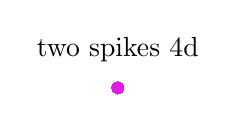
\begin{tikzpicture}

% defining custom colors
\definecolor{mycolor1}{rgb}{1,0.1,0.1}
\definecolor{mycolor2}{rgb}{0.1,1,0.1}
\definecolor{mycolor3}{rgb}{0.1,0.1,1}
\definecolor{mycolor4}{rgb}{0.1,1,1}
\definecolor{mycolor5}{rgb}{0.9,0.1,0.9}


\begin{axis}[%
view={-72}{42},
xmin=0, xmax=100,
xlabel={Number of samples},
xmajorgrids,
y dir=reverse,
ymin=-40, ymax=40,
ylabel={sample location},
ymajorgrids,
zmin=0, zmax=0.04,
zmajorgrids,
axis lines=left,
scale only axis,
width=\fwidth,
height=\fheight,
title={two spikes 4d}]
\addplot3 [
color=mycolor1,
only marks,
mark=*,
mark options={solid}
]
coordinates{
 (1,8.64397318249258,0)(2,0.94202610858281,0)(3,-8.51909224508774,0)(4,8.73504449150106,0)(5,-4.38039043088074,0)(6,-4.29661051911298,0)(7,-11.0272856023819,0)(8,3.9624682112797,0)(9,-9.64925101622627,0)(10,1.68448763331274,0)(11,-19.6535886818246,0)(12,-7.44302088643632,0)(13,-5.52306700484431,0)(14,-8.19726048957947,0)(15,11.0914180018547,0)(16,-6.14945861779946,0)(17,-2.54635294228131,0)(18,-2.6982964643979,0)(19,-16.7199406378983,0)(20,-18.7604530491713,0)(21,5.75006015878006,0)(22,-8.66133150431014,0)(23,-21.1652270104548,0)(24,-9.64465668893709,0)(25,2.12729440847614,0)(26,4.77917410863812,0)(27,1.0065773429252,0)(28,2.97433365310199,0)(29,5.70148492190659,0)(30,-16.2449561946395,0)(31,6.43442896614198,0)(32,6.81861101501212,0)(33,0.146545462976063,0)(34,-13.0154083556885,0)(35,-12.8458694199502,0)(36,8.12213221007246,0)(37,8.38548117504491,0)(38,14.2032099924033,0)(39,-9.89751963936141,0)(40,-11.8322927670026,0)(41,-4.66258701033501,0)(42,-3.65943456601606,0)(43,11.1833282594471,0)(44,-4.65614764979949,0)(45,-15.6079951442098,0)(46,-2.83103049634655,0)(47,-13.2294142478163,0)(48,-1.96238020663121,0)(49,4.19039092209372,0)(50,7.42318242363705,0)(51,-1.43031901660663,0)(52,-21.6194345485188,0)(53,-6.44226188013935,0)(54,14.3958966362552,0)(55,-8.46916703704845,0)(56,0.573396598842837,0)(57,6.43407819310009,0)(58,-6.70431031039433,0)(59,-0.0314182038723435,0)(60,3.5293137585827,0)(61,11.7950226794027,0)(62,-6.85902078686398,0)(63,16.7678943259546,0)(64,-2.55308776295612,0)(65,-6.47548492231093,0)(66,-1.82214217198884,0)(67,8.51800292262651,0)(68,-3.06550037434344,0)(69,-4.40528888444301,0)(70,-6.11471876975789,0)(71,-4.85206910127117,0)(72,11.9701928905678,0)(73,13.9478769033299,0)(74,1.65367561474691,0)(75,-5.09966956368727,0)(76,13.7771664896642,0)(77,12.9851755410422,0)(78,-1.30117041997769,0)(79,7.40248586252175,0)(80,13.320174467912,0)(81,-2.78070689182663,0)(82,-3.27992902252155,0)(83,-0.125272443409905,0)(84,9.03178709204238,0)(85,-11.1246332865596,0)(86,-8.39210796544983,0)(87,0.355343920326862,0)(88,-12.4652893677206,0)(89,8.84505037335452,0)(90,25.3833384421976,0)(91,13.1679503886664,0)(92,14.4221307180034,0)(93,14.6691939938362,0)(94,-11.0705180813558,0)(95,-4.60936138301192,0)(96,-0.202959162388906,0)(97,-0.459981798696434,0)(98,-5.44486576241684,0)(99,9.17034563222667,0)(100,-0.194183076797647,0) 
};

\addplot3 [
color=mycolor2,
only marks,
mark=*,
mark options={solid}
]
coordinates{
 (1,8.64397318249258,0)(2,8.64397318249258,0)(3,6.89742604198936,0)(4,6.89742604198936,0)(5,6.89742604198936,0)(6,7.57013560044188,0)(7,7.57013560044188,0)(8,7.57013560044188,0)(9,7.57013560044188,0)(10,6.09569612630451,0)(11,6.09569612630451,0)(12,6.09569612630451,0)(13,4.05847404385261,0)(14,4.05847404385261,0)(15,7.78838771587807,0)(16,5.74065958501997,0)(17,5.74065958501997,0)(18,10.1513655388378,0)(19,10.1513655388378,0)(20,10.1513655388378,0)(21,10.1513655388378,0)(22,12.9484160587101,0)(23,12.9484160587101,0)(24,12.8029570421,0)(25,12.8029570421,0)(26,12.8029570421,0)(27,7.79353418886505,0)(28,7.79353418886505,0)(29,7.79353418886505,0)(30,7.79353418886505,0)(31,7.79353418886505,0)(32,7.79353418886505,0)(33,7.79353418886505,0)(34,7.79353418886505,0)(35,7.79353418886505,0)(36,7.79353418886505,0)(37,8.05546429941843,0)(38,8.05546429941843,0)(39,8.05546429941843,0)(40,8.05546429941843,0)(41,8.05546429941843,0)(42,8.05546429941843,0)(43,8.05546429941843,0)(44,8.05546429941843,0)(45,8.05546429941843,0)(46,8.05546429941843,0)(47,8.05546429941843,0)(48,8.05546429941843,0)(49,8.05546429941843,0)(50,8.05546429941843,0)(51,8.05546429941843,0)(52,8.05546429941843,0)(53,8.05546429941843,0)(54,6.32383509279916,0)(55,6.32383509279916,0)(56,6.32383509279916,0)(57,6.32383509279916,0)(58,6.32383509279916,0)(59,6.32383509279916,0)(60,6.32383509279916,0)(61,6.32383509279916,0)(62,6.32383509279916,0)(63,6.32383509279916,0)(64,6.32383509279916,0)(65,6.32383509279916,0)(66,6.32383509279916,0)(67,6.32383509279916,0)(68,6.32383509279916,0)(69,6.32383509279916,0)(70,6.32383509279916,0)(71,6.32383509279916,0)(72,8.66723946845967,0)(73,8.66723946845967,0)(74,8.66723946845967,0)(75,8.66723946845967,0)(76,8.66723946845967,0)(77,11.3669821747669,0)(78,11.3669821747669,0)(79,11.3669821747669,0)(80,11.3669821747669,0)(81,11.3669821747669,0)(82,11.3669821747669,0)(83,11.3669821747669,0)(84,11.3669821747669,0)(85,11.3669821747669,0)(86,11.3669821747669,0)(87,11.3669821747669,0)(88,11.3669821747669,0)(89,11.3669821747669,0)(90,11.3669821747669,0)(91,11.3669821747669,0)(92,11.3669821747669,0)(93,11.6096037532094,0)(94,11.6096037532094,0)(95,11.6096037532094,0)(96,11.6096037532094,0)(97,11.6096037532094,0)(98,11.6096037532094,0)(99,11.6096037532094,0)(100,11.6096037532094,0) 
};

\addplot3 [
color=mycolor3,
only marks,
mark=*,
mark options={solid}
]
coordinates{
 (1,8.64397318249258,0)(2,8.64397318249258,0)(3,6.89742604198936,0)(4,6.89742604198936,0)(5,6.89742604198936,0)(6,7.57013560044188,0)(7,7.57013560044188,0)(8,7.57013560044188,0)(9,7.57013560044188,0)(10,6.09569612630451,0)(11,6.09569612630451,0)(12,6.09569612630451,0)(13,4.05847404385261,0)(14,4.05847404385261,0)(15,7.78838771587807,0)(16,5.74065958501997,0)(17,5.74065958501997,0)(18,10.1513655388378,0)(19,10.1513655388378,0)(20,10.1513655388378,0)(21,10.1513655388378,0)(22,12.9484160587101,0)(23,12.9484160587101,0)(24,12.8029570421,0)(25,12.8029570421,0)(26,12.8029570421,0)(27,7.79353418886505,0)(28,7.79353418886505,0)(29,7.79353418886505,0)(30,7.79353418886505,0)(31,7.79353418886505,0)(32,7.79353418886505,0)(33,7.79353418886505,0)(34,7.79353418886505,0)(35,7.79353418886505,0)(36,7.79353418886505,0)(37,8.05546429941843,0)(38,8.05546429941843,0)(39,8.05546429941843,0)(40,8.05546429941843,0)(41,8.05546429941843,0)(42,8.05546429941843,0)(43,8.05546429941843,0)(44,8.05546429941843,0)(45,8.05546429941843,0)(46,8.05546429941843,0)(47,8.05546429941843,0)(48,8.05546429941843,0)(49,8.05546429941843,0)(50,8.05546429941843,0)(51,8.05546429941843,0)(52,8.05546429941843,0)(53,8.05546429941843,0)(54,6.32383509279916,0)(55,6.32383509279916,0)(56,6.32383509279916,0)(57,6.32383509279916,0)(58,6.32383509279916,0)(59,6.32383509279916,0)(60,6.32383509279916,0)(61,6.32383509279916,0)(62,6.32383509279916,0)(63,6.32383509279916,0)(64,6.32383509279916,0)(65,6.32383509279916,0)(66,6.32383509279916,0)(67,6.32383509279916,0)(68,6.32383509279916,0)(69,6.32383509279916,0)(70,6.32383509279916,0)(71,6.32383509279916,0)(72,8.66723946845967,0)(73,8.66723946845967,0)(74,8.66723946845967,0)(75,8.66723946845967,0)(76,8.66723946845967,0)(77,11.3669821747669,0)(78,11.3669821747669,0)(79,11.3669821747669,0)(80,11.3669821747669,0)(81,11.3669821747669,0)(82,11.3669821747669,0)(83,11.3669821747669,0)(84,11.3669821747669,0)(85,11.3669821747669,0)(86,11.3669821747669,0)(87,11.3669821747669,0)(88,11.3669821747669,0)(89,11.3669821747669,0)(90,11.3669821747669,0)(91,11.3669821747669,0)(92,11.3669821747669,0)(93,11.6096037532094,0)(94,11.6096037532094,0)(95,11.6096037532094,0)(96,11.6096037532094,0)(97,11.6096037532094,0)(98,11.6096037532094,0)(99,11.6096037532094,0)(100,11.6096037532094,0) 
};

\addplot3 [
color=mycolor4,
only marks,
mark=*,
mark options={solid}
]
coordinates{
 (1,8.64397318249258,0)(2,-4.38039043088074,0)(3,-9.64925101622627,0)(4,-5.52306700484431,0)(5,-2.54635294228131,0)(6,5.75006015878006,0)(7,2.12729440847614,0)(8,5.70148492190659,0)(9,0.146545462976063,0)(10,8.38548117504491,0)(11,-4.66258701033501,0)(12,-15.6079951442098,0)(13,4.19039092209372,0)(14,-6.44226188013935,0)(15,6.43407819310009,0)(16,11.7950226794027,0)(17,-6.47548492231093,0)(18,-4.40528888444301,0)(19,13.9478769033299,0)(20,12.9851755410422,0)(21,-2.78070689182663,0)(22,-11.1246332865596,0)(23,8.84505037335452,0)(24,14.6691939938362,0)(25,-0.459981798696434,0)(26,7.74630170067919,0)(27,6.8593778037851,0)(28,-15.8411859791217,0)(29,-15.3211487774673,0)(30,2.71534136230341,0)(31,-5.50556055505238,0)(32,-4.27841355720601,0)(33,-12.8432806164091,0)(34,22.788714924349,0)(35,-8.33888222877994,0)(36,-9.25689568236607,0)(37,-5.61827266885125,0)(38,0.828295737128377,0)(39,-0.910346091729716,0)(40,-9.28710447028532,0)(41,0,0)(42,-9.41710232692403,0)(43,16.2075129330797,0)(44,-6.35514086344284,0)(45,-20.4726855027881,0)(46,-0.87972504507333,0)(47,-0.439787231114959,0)(48,-2.14829528926237,0)(49,-7.46695232460116,0)(50,10.0346920730319,0)(51,1.06501925298886,0)(52,-10.8651159936796,0)(53,8.58655786526147,0)(54,-3.26146433447351,0)(55,4.41829071117974,0)(56,-5.47589235578721,0)(57,-16.4297445292357,0)(58,-2.51608297481982,0)(59,-0.386248047719412,0)(60,5.20474117059437,0)(61,11.5973134212842,0)(62,-15.3281983976842,0)(63,-13.9051466783837,0)(64,3.45155795737528,0)(65,-0.480373835359512,0)(66,0.571314603916797,0)(67,8.67396987080217,0)(68,17.9522813398399,0)(69,5.22442218786417,0)(70,-5.43988057630887,0)(71,-22.6243349688659,0)(72,-0.155033585159644,0)(73,-7.30090998573805,0)(74,7.41049530589206,0)(75,15.0507321352726,0)(76,-12.7806691875923,0)(77,-4.98405983066428,0)(78,9.86615924967321,0)(79,8.53733604835799,0)(80,-1.91396023802537,0)(81,-9.65133704029641,0)(82,20.1838052497679,0)(83,-7.26842720767158,0)(84,-8.67937826619676,0)(85,4.85959542900476,0)(86,-14.8766922867241,0)(87,-11.0750411220868,0)(88,-9.18766881909361,0)(89,-7.62727133228085,0)(90,-8.55062699296247,0)(91,-6.32951970568829,0)(92,17.790376880496,0)(93,-0.235713608468783,0)(94,-5.40453938066577,0)(95,0.767236797383346,0)(96,7.55429908599643,0)(97,-13.8998730188666,0)(98,23.7101392186287,0)(99,-4.1303280502124,0)(100,15.0075011042154,0) 
};

\addplot3 [
color=mycolor5,
only marks,
mark=*,
mark options={solid}
]
coordinates{
 (1,8.64397318249258,0)(2,8.64397318249258,0)(3,6.89742604198936,0)(4,6.89742604198936,0)(5,6.89742604198936,0)(6,7.57013560044188,0)(7,7.57013560044188,0)(8,7.57013560044188,0)(9,7.57013560044188,0)(10,6.09569612630451,0)(11,6.09569612630451,0)(12,6.09569612630451,0)(13,4.05847404385261,0)(14,4.05847404385261,0)(15,7.78838771587807,0)(16,5.74065958501997,0)(17,5.74065958501997,0)(18,10.1513655388378,0)(19,10.1513655388378,0)(20,10.1513655388378,0)(21,10.1513655388378,0)(22,12.9484160587101,0)(23,12.9484160587101,0)(24,12.8029570421,0)(25,12.8029570421,0)(26,12.8029570421,0)(27,7.79353418886505,0)(28,7.79353418886505,0)(29,7.79353418886505,0)(30,7.79353418886505,0)(31,7.79353418886505,0)(32,7.79353418886505,0)(33,7.79353418886505,0)(34,7.79353418886505,0)(35,7.79353418886505,0)(36,7.79353418886505,0)(37,8.05546429941843,0)(38,8.05546429941843,0)(39,8.05546429941843,0)(40,8.05546429941843,0)(41,8.05546429941843,0)(42,8.05546429941843,0)(43,8.05546429941843,0)(44,8.05546429941843,0)(45,8.05546429941843,0)(46,8.05546429941843,0)(47,8.05546429941843,0)(48,8.05546429941843,0)(49,8.05546429941843,0)(50,8.05546429941843,0)(51,8.05546429941843,0)(52,8.05546429941843,0)(53,8.05546429941843,0)(54,6.32383509279916,0)(55,6.32383509279916,0)(56,6.32383509279916,0)(57,6.32383509279916,0)(58,6.32383509279916,0)(59,6.32383509279916,0)(60,6.32383509279916,0)(61,6.32383509279916,0)(62,6.32383509279916,0)(63,6.32383509279916,0)(64,6.32383509279916,0)(65,6.32383509279916,0)(66,6.32383509279916,0)(67,6.32383509279916,0)(68,6.32383509279916,0)(69,6.32383509279916,0)(70,6.32383509279916,0)(71,6.32383509279916,0)(72,8.66723946845967,0)(73,8.66723946845967,0)(74,8.66723946845967,0)(75,8.66723946845967,0)(76,8.66723946845967,0)(77,11.3669821747669,0)(78,11.3669821747669,0)(79,11.3669821747669,0)(80,11.3669821747669,0)(81,11.3669821747669,0)(82,11.3669821747669,0)(83,11.3669821747669,0)(84,11.3669821747669,0)(85,11.3669821747669,0)(86,11.3669821747669,0)(87,11.3669821747669,0)(88,11.3669821747669,0)(89,11.3669821747669,0)(90,11.3669821747669,0)(91,11.3669821747669,0)(92,11.3669821747669,0)(93,11.6096037532094,0)(94,11.6096037532094,0)(95,11.6096037532094,0)(96,11.6096037532094,0)(97,11.6096037532094,0)(98,11.6096037532094,0)(99,11.6096037532094,0)(100,11.6096037532094,0) 
};

\addplot3 [
color=black,
solid,
line width=2.0pt
]
coordinates{
 (101,-40,1.33830225764885e-05)(101,-39.9199199199199,1.38182046410497e-05)(101,-39.8398398398398,1.42666228042307e-05)(101,-39.7597597597598,1.47286481503254e-05)(101,-39.6796796796797,1.52046611333821e-05)(101,-39.5995995995996,1.56950517814782e-05)(101,-39.5195195195195,1.6200219904485e-05)(101,-39.4394394394394,1.6720575305353e-05)(101,-39.3593593593594,1.72565379949497e-05)(101,-39.2792792792793,1.7808538410479e-05)(101,-39.1991991991992,1.83770176375138e-05)(101,-39.1191191191191,1.89624276356684e-05)(101,-39.039039039039,1.95652314679408e-05)(101,-38.958958958959,2.01859035337517e-05)(101,-38.8788788788789,2.08249298057069e-05)(101,-38.7987987987988,2.14828080701089e-05)(101,-38.7187187187187,2.21600481712426e-05)(101,-38.6386386386386,2.285717225946e-05)(101,-38.5585585585586,2.35747150430845e-05)(101,-38.4784784784785,2.43132240441603e-05)(101,-38.3983983983984,2.50732598580649e-05)(101,-38.3183183183183,2.58553964170059e-05)(101,-38.2382382382382,2.66602212574213e-05)(101,-38.1581581581582,2.74883357912987e-05)(101,-38.0780780780781,2.83403555814326e-05)(101,-37.997997997998,2.92169106206323e-05)(101,-37.9179179179179,3.01186456148956e-05)(101,-37.8378378378378,3.104622027056e-05)(101,-37.7577577577578,3.20003095854415e-05)(101,-37.6776776776777,3.29816041439723e-05)(101,-37.5975975975976,3.39908104163431e-05)(101,-37.5175175175175,3.50286510616579e-05)(101,-37.4374374374374,3.60958652351047e-05)(101,-37.3573573573574,3.71932088991451e-05)(101,-37.2772772772773,3.8321455138726e-05)(101,-37.1971971971972,3.94813944805093e-05)(101,-37.1171171171171,4.06738352161196e-05)(101,-37.037037037037,4.18996037294058e-05)(101,-36.956956956957,4.31595448277079e-05)(101,-36.8768768768769,4.4454522077123e-05)(101,-36.7967967967968,4.57854181417587e-05)(101,-36.7167167167167,4.71531351269623e-05)(101,-36.6366366366366,4.85585949265103e-05)(101,-36.5565565565566,5.00027395737409e-05)(101,-36.4764764764765,5.14865315966113e-05)(101,-36.3963963963964,5.30109543766577e-05)(101,-36.3163163163163,5.45770125118335e-05)(101,-36.2362362362362,5.61857321831992e-05)(101,-36.1561561561562,5.78381615254348e-05)(101,-36.0760760760761,5.95353710011453e-05)(101,-35.995995995996,6.12784537789192e-05)(101,-35.9159159159159,6.30685261151104e-05)(101,-35.8358358358358,6.49067277392972e-05)(101,-35.7557557557558,6.67942222433795e-05)(101,-35.6756756756757,6.87321974742665e-05)(101,-35.5955955955956,7.07218659301082e-05)(101,-35.5155155155155,7.27644651600165e-05)(101,-35.4354354354354,7.48612581672246e-05)(101,-35.3553553553554,7.70135338156225e-05)(101,-35.2752752752753,7.9222607239612e-05)(101,-35.1951951951952,8.1489820257214e-05)(101,-35.1151151151151,8.38165417863602e-05)(101,-35.035035035035,8.62041682643007e-05)(101,-34.954954954955,8.86541240700501e-05)(101,-34.8748748748749,9.11678619497959e-05)(101,-34.7947947947948,9.37468634451866e-05)(101,-34.7147147147147,9.63926393244148e-05)(101,-34.6346346346346,9.91067300160058e-05)(101,-34.5545545545546,0.00010189070604522)(101,-34.4744744744745,0.000104746168472971)(101,-34.3943943943944,0.00010767474933716)(101,-34.3143143143143,0.000110678112096323)(101,-34.2342342342342,0.000113757952075483)(101,-34.1541541541542,0.000116915996914087)(101,-34.0740740740741,0.000120154007015926)(101,-33.993993993994,0.000123473776000907)(101,-33.9139139139139,0.000126877131158549)(101,-33.8338338338338,0.000130365933903088)(101,-33.7537537537538,0.000133942080230046)(101,-33.6736736736737,0.000137607501174126)(101,-33.5935935935936,0.0001413641632683)(101,-33.5135135135135,0.000145214069003937)(101,-33.4334334334334,0.00014915925729182)(101,-33.3533533533534,0.000153201803923895)(101,-33.2732732732733,0.000157343822035606)(101,-33.1931931931932,0.000161587462568624)(101,-33.1131131131131,0.000165934914733831)(101,-33.033033033033,0.000170388406474362)(101,-32.952952952953,0.000174950204928538)(101,-32.8728728728729,0.000179622616892505)(101,-32.7927927927928,0.000184407989282385)(101,-32.7127127127127,0.000189308709595757)(101,-32.6326326326326,0.000194327206372254)(101,-32.5525525525526,0.000199465949653091)(101,-32.4724724724725,0.000204727451439301)(101,-32.3923923923924,0.000210114266148476)(101,-32.3123123123123,0.000215628991069791)(101,-32.2322322322322,0.000221274266817093)(101,-32.1521521521522,0.000227052777779814)(101,-32.0720720720721,0.000232967252571501)(101,-31.991991991992,0.000239020464475689)(101,-31.9119119119119,0.000245215231888918)(101,-31.8318318318318,0.000251554418760605)(101,-31.7517517517518,0.000258040935029545)(101,-31.6716716716717,0.000264677737056775)(101,-31.5915915915916,0.000271467828054534)(101,-31.5115115115115,0.000278414258511061)(101,-31.4314314314314,0.000285520126610952)(101,-31.3513513513514,0.000292788578650791)(101,-31.2712712712713,0.000300222809449793)(101,-31.1911911911912,0.000307826062755151)(101,-31.1111111111111,0.000315601631641804)(101,-31.031031031031,0.000323552858906328)(101,-30.950950950951,0.000331683137454643)(101,-30.8708708708709,0.000339995910683238)(101,-30.7907907907908,0.000348494672853595)(101,-30.7107107107107,0.000357182969459489)(101,-30.6306306306306,0.000366064397586863)(101,-30.5505505505506,0.000375142606265932)(101,-30.4704704704705,0.000384421296815189)(101,-30.3903903903904,0.000393904223176991)(101,-30.3103103103103,0.000403595192244368)(101,-30.2302302302302,0.000413498064178719)(101,-30.1501501501502,0.000423616752718052)(101,-30.0700700700701,0.000433955225475398)(101,-29.98998998999,0.000444517504227068)(101,-29.9099099099099,0.000455307665190355)(101,-29.8298298298298,0.000466329839290368)(101,-29.7497497497497,0.000477588212415564)(101,-29.6696696696697,0.000489087025661667)(101,-29.5895895895896,0.000500830575563558)(101,-29.5095095095095,0.000512823214314763)(101,-29.4294294294294,0.000525069349974172)(101,-29.3493493493493,0.000537573446659573)(101,-29.2692692692693,0.000550340024727644)(101,-29.1891891891892,0.000563373660939975)(101,-29.1091091091091,0.00057667898861475)(101,-29.029029029029,0.000590260697763673)(101,-28.9489489489489,0.000604123535213746)(101,-28.8688688688689,0.000618272304713484)(101,-28.7887887887888,0.000632711867023164)(101,-28.7087087087087,0.000647447139988702)(101,-28.6286286286286,0.000662483098598742)(101,-28.5485485485485,0.000677824775024529)(101,-28.4684684684685,0.00069347725864219)(101,-28.3883883883884,0.000709445696036946)(101,-28.3083083083083,0.000725735290988892)(101,-28.2282282282282,0.000742351304439893)(101,-28.1481481481481,0.000759299054441176)(101,-28.0680680680681,0.00077658391608121)(101,-27.987987987988,0.000794211321393438)(101,-27.9079079079079,0.000812186759243431)(101,-27.8278278278278,0.000830515775195072)(101,-27.7477477477477,0.000849203971355292)(101,-27.6676676676677,0.000868257006197)(101,-27.5875875875876,0.000887680594359711)(101,-27.5075075075075,0.00090748050642751)(101,-27.4274274274274,0.000927662568683897)(101,-27.3473473473473,0.0009482326628431)(101,-27.2672672672673,0.000969196725757424)(101,-27.1871871871872,0.000990560749100247)(101,-27.1071071071071,0.00101233077902421)(101,-27.027027027027,0.00103451291579421)(101,-26.9469469469469,0.00105711331339476)(101,-26.8668668668669,0.00108013817911136)(101,-26.7867867867868,0.0011035937730854)(101,-26.7067067067067,0.00112748640784219)(101,-26.6266266266266,0.00115182244779185)(101,-26.5465465465465,0.00117660830870247)(101,-26.4664664664665,0.00120185045714527)(101,-26.3863863863864,0.00122755540991133)(101,-26.3063063063063,0.00125372973339956)(101,-26.2262262262262,0.00128038004297541)(101,-26.1461461461461,0.00130751300230007)(101,-26.0660660660661,0.00133513532262973)(101,-25.985985985986,0.00136325376208454)(101,-25.9059059059059,0.00139187512488693)(101,-25.8258258258258,0.0014210062605689)(101,-25.7457457457457,0.00145065406314803)(101,-25.6656656656657,0.00148082547027168)(101,-25.5855855855856,0.00151152746232934)(101,-25.5055055055055,0.00154276706153247)(101,-25.4254254254254,0.00157455133096184)(101,-25.3453453453453,0.00160688737358179)(101,-25.2652652652653,0.0016397823312213)(101,-25.1851851851852,0.00167324338352152)(101,-25.1051051051051,0.00170727774684939)(101,-25.025025025025,0.00174189267317727)(101,-24.9449449449449,0.00177709544892815)(101,-24.8648648648649,0.00181289339378627)(101,-24.7847847847848,0.00184929385947285)(101,-24.7047047047047,0.00188630422848682)(101,-24.6246246246246,0.00192393191281025)(101,-24.5445445445445,0.00196218435257817)(101,-24.4644644644645,0.00200106901471285)(101,-24.3843843843844,0.0020405933915221)(101,-24.3043043043043,0.0020807649992616)(101,-24.2242242242242,0.00212159137666093)(101,-24.1441441441441,0.00216308008341344)(101,-24.0640640640641,0.00220523869862944)(101,-23.983983983984,0.00224807481925294)(101,-23.9039039039039,0.0022915960584417)(101,-23.8238238238238,0.00233581004391047)(101,-23.7437437437437,0.0023807244162374)(101,-23.6636636636637,0.00242634682713357)(101,-23.5835835835836,0.00247268493767558)(101,-23.5035035035035,0.00251974641650119)(101,-23.4234234234234,0.00256753893796796)(101,-23.3433433433433,0.00261607018027502)(101,-23.2632632632633,0.00266534782354776)(101,-23.1831831831832,0.00271537954788581)(101,-23.1031031031031,0.00276617303137407)(101,-23.023023023023,0.00281773594805703)(101,-22.9429429429429,0.00287007596587648)(101,-22.8628628628629,0.00292320074457259)(101,-22.7827827827828,0.0029771179335487)(101,-22.7027027027027,0.00303183516969979)(101,-22.6226226226226,0.00308736007520491)(101,-22.5425425425425,0.00314370025528369)(101,-22.4624624624625,0.00320086329591723)(101,-22.3823823823824,0.00325885676153351)(101,-22.3023023023023,0.00331768819265761)(101,-22.2222222222222,0.00337736510352706)(101,-22.1421421421421,0.00343789497967251)(101,-22.0620620620621,0.00349928527546413)(101,-21.981981981982,0.00356154341162401)(101,-21.9019019019019,0.00362467677270497)(101,-21.8218218218218,0.00368869270453615)(101,-21.7417417417417,0.00375359851163568)(101,-21.6616616616617,0.00381940145459099)(101,-21.5815815815816,0.00388610874740723)(101,-21.5015015015015,0.00395372755482399)(101,-21.4214214214214,0.0040222649896012)(101,-21.3413413413413,0.00409172810977437)(101,-21.2612612612613,0.00416212391588003)(101,-21.1811811811812,0.00423345934815158)(101,-21.1011011011011,0.00430574128368641)(101,-21.021021021021,0.00437897653358481)(101,-20.9409409409409,0.00445317184006117)(101,-20.8608608608609,0.00452833387352837)(101,-20.7807807807808,0.00460446922965576)(101,-20.7007007007007,0.00468158442640166)(101,-20.6206206206206,0.00475968590102091)(101,-20.5405405405405,0.00483878000704834)(101,-20.4604604604605,0.00491887301125894)(101,-20.3803803803804,0.00499997109060533)(101,-20.3003003003003,0.00508208032913362)(101,-20.2202202202202,0.00516520671487824)(101,-20.1401401401401,0.00524935613673682)(101,-20.0600600600601,0.0053345343813258)(101,-19.97997997998,0.00542074712981784)(101,-19.8998998998999,0.00550799995476186)(101,-19.8198198198198,0.00559629831688667)(101,-19.7397397397397,0.00568564756188931)(101,-19.6596596596597,0.00577605291720876)(101,-19.5795795795796,0.0058675194887865)(101,-19.4994994994995,0.00596005225781458)(101,-19.4194194194194,0.00605365607747232)(101,-19.3393393393393,0.0061483356696531)(101,-19.2592592592593,0.0062440956216817)(101,-19.1791791791792,0.00634094038302401)(101,-19.0990990990991,0.00643887426198963)(101,-19.019019019019,0.00653790142242912)(101,-18.9389389389389,0.00663802588042656)(101,-18.8588588588589,0.00673925150098903)(101,-18.7787787787788,0.00684158199473404)(101,-18.6986986986987,0.00694502091457626)(101,-18.6186186186186,0.00704957165241465)(101,-18.5385385385385,0.00715523743582165)(101,-18.4584584584585,0.00726202132473521)(101,-18.3783783783784,0.00736992620815557)(101,-18.2982982982983,0.00747895480084762)(101,-18.2182182182182,0.00758910964005057)(101,-18.1381381381381,0.00770039308219614)(101,-18.0580580580581,0.00781280729963669)(101,-17.977977977978,0.00792635427738473)(101,-17.8978978978979,0.00804103580986525)(101,-17.8178178178178,0.00815685349768226)(101,-17.7377377377377,0.00827380874440108)(101,-17.6576576576577,0.00839190275334777)(101,-17.5775775775776,0.00851113652442723)(101,-17.4974974974975,0.0086315108509615)(101,-17.4174174174174,0.00875302631654975)(101,-17.3373373373373,0.00887568329195139)(101,-17.2572572572573,0.00899948193199405)(101,-17.1771771771772,0.00912442217250772)(101,-17.0970970970971,0.00925050372728685)(101,-17.017017017017,0.00937772608508176)(101,-16.9369369369369,0.00950608850662112)(101,-16.8568568568569,0.00963559002166691)(101,-16.7767767767768,0.00976622942610364)(101,-16.6966966966967,0.0098980052790632)(101,-16.6166166166166,0.0100309159000872)(101,-16.5365365365365,0.0101649593663279)(101,-16.4564564564565,0.0103001335097907)(101,-16.3763763763764,0.010436435914617)(101,-16.2962962962963,0.0105738639144131)(101,-16.2162162162162,0.0107124145896225)(101,-16.1361361361361,0.0108520847649465)(101,-16.0560560560561,0.010992871006813)(101,-15.975975975976,0.0111347696208955)(101,-15.8958958958959,0.0112777766496842)(101,-15.8158158158158,0.0114218878701105)(101,-15.7357357357357,0.0115670987912262)(101,-15.6556556556557,0.0117134046519405)(101,-15.5755755755756,0.011860800418814)(101,-15.4954954954955,0.0120092807839133)(101,-15.4154154154154,0.0121588401627275)(101,-15.3353353353353,0.0123094726921466)(101,-15.2552552552553,0.0124611722285057)(101,-15.1751751751752,0.012613932345695)(101,-15.0950950950951,0.0127677463333369)(101,-15.015015015015,0.0129226071950339)(101,-14.9349349349349,0.0130785076466857)(101,-14.8548548548549,0.0132354401148798)(101,-14.7747747747748,0.0133933967353555)(101,-14.6946946946947,0.013552369351543)(101,-14.6146146146146,0.0137123495131801)(101,-14.5345345345345,0.013873328475006)(101,-14.4544544544545,0.0140352971955359)(101,-14.3743743743744,0.0141982463359159)(101,-14.2942942942943,0.0143621662588612)(101,-14.2142142142142,0.014527047027677)(101,-14.1341341341341,0.0146928784053658)(101,-14.0540540540541,0.0148596498538208)(101,-13.973973973974,0.0150273505331067)(101,-13.8938938938939,0.0151959693008306)(101,-13.8138138138138,0.0153654947116025)(101,-13.7337337337337,0.0155359150165875)(101,-13.6536536536537,0.0157072181631514)(101,-13.5735735735736,0.0158793917945997)(101,-13.4934934934935,0.0160524232500122)(101,-13.4134134134134,0.016226299564173)(101,-13.3333333333333,0.0164010074675994)(101,-13.2532532532533,0.0165765333866673)(101,-13.1731731731732,0.0167528634438376)(101,-13.0930930930931,0.0169299834579821)(101,-13.013013013013,0.017107878944811)(101,-12.9329329329329,0.0172865351174024)(101,-12.8528528528529,0.0174659368868355)(101,-12.7727727727728,0.0176460688629273)(101,-12.6926926926927,0.0178269153550739)(101,-12.6126126126126,0.018008460373198)(101,-12.5325325325325,0.0181906876288021)(101,-12.4524524524525,0.0183735805361283)(101,-12.3723723723724,0.0185571222134271)(101,-12.2922922922923,0.0187412954843324)(101,-12.2122122122122,0.018926082879347)(101,-12.1321321321321,0.0191114666374361)(101,-12.0520520520521,0.0192974287077311)(101,-11.971971971972,0.0194839507513435)(101,-11.8918918918919,0.019671014143289)(101,-11.8118118118118,0.0198585999745227)(101,-11.7317317317317,0.0200466890540856)(101,-11.6516516516517,0.0202352619113618)(101,-11.5715715715716,0.0204242987984477)(101,-11.4914914914915,0.0206137796926331)(101,-11.4114114114114,0.0208036842989938)(101,-11.3313313313313,0.0209939920530956)(101,-11.2512512512513,0.021184682123811)(101,-11.1711711711712,0.021375733416247)(101,-11.0910910910911,0.0215671245747847)(101,-11.011011011011,0.0217588339862305)(101,-10.9309309309309,0.0219508397830784)(101,-10.8508508508509,0.0221431198468836)(101,-10.7707707707708,0.0223356518117463)(101,-10.6906906906907,0.0225284130679063)(101,-10.6106106106106,0.022721380765447)(101,-10.5305305305305,0.0229145318181096)(101,-10.4504504504505,0.0231078429072154)(101,-10.3703703703704,0.0233012904856966)(101,-10.2902902902903,0.0234948507822352)(101,-10.2102102102102,0.0236884998055083)(101,-10.1301301301301,0.0238822133485401)(101,-10.0500500500501,0.024075966993159)(101,-9.96996996996997,0.0242697361145593)(101,-9.88988988988989,0.0244634958859672)(101,-9.80980980980981,0.0246572212834085)(101,-9.72972972972973,0.0248508870905785)(101,-9.64964964964965,0.025044467903813)(101,-9.56956956956957,0.0252379381371581)(101,-9.48948948948949,0.0254312720275384)(101,-9.40940940940941,0.0256244436400228)(101,-9.32932932932933,0.0258174268731856)(101,-9.24924924924925,0.0260101954645623)(101,-9.16916916916917,0.0262027229961987)(101,-9.08908908908909,0.0263949829002911)(101,-9.00900900900901,0.0265869484649171)(101,-8.92892892892893,0.0267785928398552)(101,-8.84884884884885,0.0269698890424904)(101,-8.76876876876877,0.0271608099638066)(101,-8.68868868868869,0.0273513283744617)(101,-8.60860860860861,0.0275414169309444)(101,-8.52852852852853,0.0277310481818124)(101,-8.44844844844845,0.0279201945740075)(101,-8.36836836836837,0.0281088284592474)(101,-8.28828828828829,0.028296922100493)(101,-8.20820820820821,0.0284844476784867)(101,-8.12812812812813,0.0286713772983616)(101,-8.04804804804805,0.0288576829963198)(101,-7.96796796796797,0.0290433367463758)(101,-7.88788788788789,0.0292283104671645)(101,-7.80780780780781,0.0294125760288111)(101,-7.72772772772772,0.0295961052598603)(101,-7.64764764764764,0.029778869954263)(101,-7.56756756756756,0.0299608418784177)(101,-7.48748748748748,0.0301419927782648)(101,-7.4074074074074,0.0303222943864308)(101,-7.32732732732732,0.0305017184294204)(101,-7.24724724724724,0.0306802366348536)(101,-7.16716716716716,0.0308578207387456)(101,-7.08708708708708,0.0310344424928268)(101,-7.007007007007,0.0312100736719007)(101,-6.92692692692692,0.0313846860812361)(101,-6.84684684684684,0.031558251563992)(101,-6.76676676676676,0.0317307420086723)(101,-6.68668668668668,0.0319021293566066)(101,-6.6066066066066,0.032072385609456)(101,-6.52652652652652,0.0322414828367396)(101,-6.44644644644644,0.0324093931833804)(101,-6.36636636636636,0.0325760888772662)(101,-6.28628628628628,0.0327415422368237)(101,-6.2062062062062,0.0329057256786028)(101,-6.12612612612612,0.0330686117248681)(101,-6.04604604604604,0.033230173011195)(101,-5.96596596596596,0.0333903822940662)(101,-5.88588588588588,0.0335492124584683)(101,-5.8058058058058,0.0337066365254824)(101,-5.72572572572572,0.0338626276598684)(101,-5.64564564564564,0.0340171591776383)(101,-5.56556556556556,0.0341702045536168)(101,-5.48548548548548,0.0343217374289848)(101,-5.4054054054054,0.0344717316188045)(101,-5.32532532532532,0.0346201611195215)(101,-5.24524524524524,0.0347670001164422)(101,-5.16516516516516,0.0349122229911825)(101,-5.08508508508508,0.0350558043290856)(101,-5.005005005005,0.0351977189266053)(101,-4.92492492492492,0.0353379417986526)(101,-4.84484484484484,0.0354764481859011)(101,-4.76476476476476,0.0356132135620502)(101,-4.68468468468468,0.0357482136410418)(101,-4.6046046046046,0.0358814243842273)(101,-4.52452452452452,0.0360128220074839)(101,-4.44444444444444,0.0361423829882743)(101,-4.36436436436436,0.0362700840726495)(101,-4.28428428428428,0.0363959022821904)(101,-4.2042042042042,0.0365198149208855)(101,-4.12412412412412,0.0366417995819425)(101,-4.04404404404404,0.03676183415453)(101,-3.96396396396396,0.0368798968304465)(101,-3.88388388388388,0.0369959661107154)(101,-3.8038038038038,0.037110020812101)(101,-3.72372372372372,0.0372220400735444)(101,-3.64364364364364,0.0373320033625156)(101,-3.56356356356356,0.0374398904812801)(101,-3.48348348348348,0.0375456815730761)(101,-3.4034034034034,0.0376493571282005)(101,-3.32332332332332,0.0377508979900006)(101,-3.24324324324324,0.0378502853607702)(101,-3.16316316316316,0.0379475008075448)(101,-3.08308308308308,0.0380425262677969)(101,-3.003003003003,0.0381353440550259)(101,-2.92292292292292,0.0382259368642425)(101,-2.84284284284284,0.038314287777343)(101,-2.76276276276276,0.0384003802683735)(101,-2.68268268268268,0.03848419820868)(101,-2.6026026026026,0.0385657258719425)(101,-2.52252252252252,0.0386449479390916)(101,-2.44244244244244,0.0387218495031049)(101,-2.36236236236236,0.0387964160736804)(101,-2.28228228228228,0.038868633581787)(101,-2.2022022022022,0.0389384883840873)(101,-2.12212212212212,0.0390059672672329)(101,-2.04204204204204,0.0390710574520297)(101,-1.96196196196196,0.0391337465974705)(101,-1.88188188188188,0.039194022804635)(101,-1.8018018018018,0.0392518746204527)(101,-1.72172172172172,0.0393072910413305)(101,-1.64164164164164,0.0393602615166401)(101,-1.56156156156156,0.0394107759520657)(101,-1.48148148148148,0.0394588247128102)(101,-1.4014014014014,0.0395043986266573)(101,-1.32132132132132,0.03954748898689)(101,-1.24124124124124,0.0395880875550626)(101,-1.16116116116116,0.0396261865636259)(101,-1.08108108108108,0.0396617787184037)(101,-1.001001001001,0.0396948572009207)(101,-0.920920920920921,0.0397254156705792)(101,-0.840840840840841,0.0397534482666846)(101,-0.76076076076076,0.039778949610319)(101,-0.68068068068068,0.039801914806061)(101,-0.6006006006006,0.0398223394435522)(101,-0.52052052052052,0.0398402195989086)(101,-0.44044044044044,0.0398555518359772)(101,-0.36036036036036,0.0398683332074364)(101,-0.28028028028028,0.0398785612557403)(101,-0.2002002002002,0.0398862340139061)(101,-0.12012012012012,0.0398913500061449)(101,-0.04004004004004,0.0398939082483343)(101,0.04004004004004,0.0398939082483343)(101,0.12012012012012,0.0398913500061449)(101,0.2002002002002,0.0398862340139061)(101,0.28028028028028,0.0398785612557403)(101,0.36036036036036,0.0398683332074364)(101,0.44044044044044,0.0398555518359772)(101,0.52052052052052,0.0398402195989086)(101,0.6006006006006,0.0398223394435522)(101,0.68068068068068,0.039801914806061)(101,0.76076076076076,0.039778949610319)(101,0.840840840840841,0.0397534482666846)(101,0.920920920920921,0.0397254156705792)(101,1.001001001001,0.0396948572009207)(101,1.08108108108108,0.0396617787184037)(101,1.16116116116116,0.0396261865636259)(101,1.24124124124124,0.0395880875550626)(101,1.32132132132132,0.03954748898689)(101,1.4014014014014,0.0395043986266573)(101,1.48148148148148,0.0394588247128102)(101,1.56156156156156,0.0394107759520657)(101,1.64164164164164,0.0393602615166401)(101,1.72172172172172,0.0393072910413305)(101,1.8018018018018,0.0392518746204527)(101,1.88188188188188,0.039194022804635)(101,1.96196196196196,0.0391337465974705)(101,2.04204204204204,0.0390710574520297)(101,2.12212212212212,0.0390059672672329)(101,2.2022022022022,0.0389384883840873)(101,2.28228228228228,0.038868633581787)(101,2.36236236236236,0.0387964160736804)(101,2.44244244244244,0.0387218495031049)(101,2.52252252252252,0.0386449479390916)(101,2.6026026026026,0.0385657258719425)(101,2.68268268268268,0.03848419820868)(101,2.76276276276276,0.0384003802683735)(101,2.84284284284284,0.038314287777343)(101,2.92292292292292,0.0382259368642425)(101,3.003003003003,0.0381353440550259)(101,3.08308308308308,0.0380425262677969)(101,3.16316316316316,0.0379475008075448)(101,3.24324324324324,0.0378502853607702)(101,3.32332332332332,0.0377508979900006)(101,3.4034034034034,0.0376493571282005)(101,3.48348348348348,0.0375456815730761)(101,3.56356356356356,0.0374398904812801)(101,3.64364364364364,0.0373320033625156)(101,3.72372372372372,0.0372220400735444)(101,3.8038038038038,0.037110020812101)(101,3.88388388388388,0.0369959661107154)(101,3.96396396396396,0.0368798968304465)(101,4.04404404404404,0.03676183415453)(101,4.12412412412412,0.0366417995819425)(101,4.2042042042042,0.0365198149208855)(101,4.28428428428428,0.0363959022821904)(101,4.36436436436436,0.0362700840726495)(101,4.44444444444444,0.0361423829882743)(101,4.52452452452452,0.0360128220074839)(101,4.6046046046046,0.0358814243842273)(101,4.68468468468468,0.0357482136410418)(101,4.76476476476476,0.0356132135620502)(101,4.84484484484484,0.0354764481859011)(101,4.92492492492492,0.0353379417986526)(101,5.005005005005,0.0351977189266053)(101,5.08508508508508,0.0350558043290856)(101,5.16516516516516,0.0349122229911825)(101,5.24524524524524,0.0347670001164422)(101,5.32532532532532,0.0346201611195215)(101,5.4054054054054,0.0344717316188045)(101,5.48548548548548,0.0343217374289848)(101,5.56556556556556,0.0341702045536168)(101,5.64564564564564,0.0340171591776383)(101,5.72572572572572,0.0338626276598684)(101,5.8058058058058,0.0337066365254824)(101,5.88588588588588,0.0335492124584683)(101,5.96596596596596,0.0333903822940662)(101,6.04604604604604,0.033230173011195)(101,6.12612612612612,0.0330686117248681)(101,6.2062062062062,0.0329057256786028)(101,6.28628628628628,0.0327415422368237)(101,6.36636636636636,0.0325760888772662)(101,6.44644644644644,0.0324093931833804)(101,6.52652652652652,0.0322414828367396)(101,6.6066066066066,0.032072385609456)(101,6.68668668668668,0.0319021293566066)(101,6.76676676676676,0.0317307420086723)(101,6.84684684684684,0.031558251563992)(101,6.92692692692692,0.0313846860812361)(101,7.007007007007,0.0312100736719007)(101,7.08708708708708,0.0310344424928268)(101,7.16716716716716,0.0308578207387456)(101,7.24724724724724,0.0306802366348536)(101,7.32732732732732,0.0305017184294204)(101,7.4074074074074,0.0303222943864308)(101,7.48748748748748,0.0301419927782648)(101,7.56756756756756,0.0299608418784177)(101,7.64764764764764,0.029778869954263)(101,7.72772772772772,0.0295961052598603)(101,7.80780780780781,0.0294125760288111)(101,7.88788788788789,0.0292283104671645)(101,7.96796796796797,0.0290433367463758)(101,8.04804804804805,0.0288576829963198)(101,8.12812812812813,0.0286713772983616)(101,8.20820820820821,0.0284844476784867)(101,8.28828828828829,0.028296922100493)(101,8.36836836836837,0.0281088284592474)(101,8.44844844844845,0.0279201945740075)(101,8.52852852852853,0.0277310481818125)(101,8.60860860860861,0.0275414169309444)(101,8.68868868868869,0.0273513283744617)(101,8.76876876876877,0.0271608099638066)(101,8.84884884884885,0.0269698890424904)(101,8.92892892892893,0.0267785928398552)(101,9.00900900900901,0.0265869484649172)(101,9.08908908908909,0.0263949829002911)(101,9.16916916916917,0.0262027229961987)(101,9.24924924924925,0.0260101954645624)(101,9.32932932932933,0.0258174268731856)(101,9.40940940940941,0.0256244436400228)(101,9.48948948948949,0.0254312720275385)(101,9.56956956956957,0.0252379381371581)(101,9.64964964964965,0.0250444679038131)(101,9.72972972972973,0.0248508870905785)(101,9.80980980980981,0.0246572212834085)(101,9.88988988988989,0.0244634958859673)(101,9.96996996996997,0.0242697361145594)(101,10.0500500500501,0.024075966993159)(101,10.1301301301301,0.0238822133485401)(101,10.2102102102102,0.0236884998055083)(101,10.2902902902903,0.0234948507822352)(101,10.3703703703704,0.0233012904856966)(101,10.4504504504505,0.0231078429072154)(101,10.5305305305305,0.0229145318181096)(101,10.6106106106106,0.022721380765447)(101,10.6906906906907,0.0225284130679062)(101,10.7707707707708,0.0223356518117463)(101,10.8508508508509,0.0221431198468836)(101,10.9309309309309,0.0219508397830784)(101,11.011011011011,0.0217588339862305)(101,11.0910910910911,0.0215671245747847)(101,11.1711711711712,0.021375733416247)(101,11.2512512512513,0.021184682123811)(101,11.3313313313313,0.0209939920530956)(101,11.4114114114114,0.0208036842989938)(101,11.4914914914915,0.0206137796926331)(101,11.5715715715716,0.0204242987984477)(101,11.6516516516517,0.0202352619113618)(101,11.7317317317317,0.0200466890540856)(101,11.8118118118118,0.0198585999745227)(101,11.8918918918919,0.019671014143289)(101,11.971971971972,0.0194839507513435)(101,12.0520520520521,0.0192974287077311)(101,12.1321321321321,0.0191114666374361)(101,12.2122122122122,0.018926082879347)(101,12.2922922922923,0.0187412954843324)(101,12.3723723723724,0.0185571222134271)(101,12.4524524524525,0.0183735805361283)(101,12.5325325325325,0.018190687628802)(101,12.6126126126126,0.018008460373198)(101,12.6926926926927,0.0178269153550739)(101,12.7727727727728,0.0176460688629273)(101,12.8528528528529,0.0174659368868355)(101,12.9329329329329,0.0172865351174024)(101,13.013013013013,0.017107878944811)(101,13.0930930930931,0.0169299834579821)(101,13.1731731731732,0.0167528634438376)(101,13.2532532532533,0.0165765333866673)(101,13.3333333333333,0.0164010074675993)(101,13.4134134134134,0.016226299564173)(101,13.4934934934935,0.0160524232500122)(101,13.5735735735736,0.0158793917945997)(101,13.6536536536537,0.0157072181631514)(101,13.7337337337337,0.0155359150165875)(101,13.8138138138138,0.0153654947116025)(101,13.8938938938939,0.0151959693008306)(101,13.973973973974,0.0150273505331067)(101,14.0540540540541,0.0148596498538208)(101,14.1341341341341,0.0146928784053658)(101,14.2142142142142,0.014527047027677)(101,14.2942942942943,0.0143621662588612)(101,14.3743743743744,0.0141982463359159)(101,14.4544544544545,0.0140352971955359)(101,14.5345345345345,0.013873328475006)(101,14.6146146146146,0.0137123495131801)(101,14.6946946946947,0.013552369351543)(101,14.7747747747748,0.0133933967353555)(101,14.8548548548549,0.0132354401148798)(101,14.9349349349349,0.0130785076466857)(101,15.015015015015,0.0129226071950339)(101,15.0950950950951,0.0127677463333369)(101,15.1751751751752,0.012613932345695)(101,15.2552552552553,0.0124611722285057)(101,15.3353353353353,0.0123094726921466)(101,15.4154154154154,0.0121588401627275)(101,15.4954954954955,0.0120092807839133)(101,15.5755755755756,0.011860800418814)(101,15.6556556556557,0.0117134046519405)(101,15.7357357357357,0.0115670987912262)(101,15.8158158158158,0.0114218878701105)(101,15.8958958958959,0.0112777766496842)(101,15.975975975976,0.0111347696208955)(101,16.0560560560561,0.010992871006813)(101,16.1361361361361,0.0108520847649465)(101,16.2162162162162,0.0107124145896225)(101,16.2962962962963,0.0105738639144131)(101,16.3763763763764,0.010436435914617)(101,16.4564564564565,0.0103001335097907)(101,16.5365365365365,0.0101649593663279)(101,16.6166166166166,0.0100309159000872)(101,16.6966966966967,0.0098980052790632)(101,16.7767767767768,0.00976622942610364)(101,16.8568568568569,0.00963559002166691)(101,16.9369369369369,0.00950608850662112)(101,17.017017017017,0.00937772608508176)(101,17.0970970970971,0.00925050372728685)(101,17.1771771771772,0.00912442217250772)(101,17.2572572572573,0.00899948193199405)(101,17.3373373373373,0.00887568329195139)(101,17.4174174174174,0.00875302631654975)(101,17.4974974974975,0.0086315108509615)(101,17.5775775775776,0.00851113652442723)(101,17.6576576576577,0.00839190275334777)(101,17.7377377377377,0.00827380874440108)(101,17.8178178178178,0.00815685349768226)(101,17.8978978978979,0.00804103580986525)(101,17.977977977978,0.00792635427738473)(101,18.0580580580581,0.00781280729963669)(101,18.1381381381381,0.00770039308219614)(101,18.2182182182182,0.00758910964005057)(101,18.2982982982983,0.00747895480084762)(101,18.3783783783784,0.00736992620815557)(101,18.4584584584585,0.00726202132473521)(101,18.5385385385385,0.00715523743582165)(101,18.6186186186186,0.00704957165241465)(101,18.6986986986987,0.00694502091457626)(101,18.7787787787788,0.00684158199473404)(101,18.8588588588589,0.00673925150098903)(101,18.9389389389389,0.00663802588042656)(101,19.019019019019,0.00653790142242912)(101,19.0990990990991,0.00643887426198963)(101,19.1791791791792,0.00634094038302401)(101,19.2592592592593,0.0062440956216817)(101,19.3393393393393,0.0061483356696531)(101,19.4194194194194,0.00605365607747232)(101,19.4994994994995,0.00596005225781458)(101,19.5795795795796,0.0058675194887865)(101,19.6596596596597,0.00577605291720876)(101,19.7397397397397,0.00568564756188931)(101,19.8198198198198,0.00559629831688667)(101,19.8998998998999,0.00550799995476186)(101,19.97997997998,0.00542074712981784)(101,20.0600600600601,0.0053345343813258)(101,20.1401401401401,0.00524935613673682)(101,20.2202202202202,0.00516520671487824)(101,20.3003003003003,0.00508208032913362)(101,20.3803803803804,0.00499997109060533)(101,20.4604604604605,0.00491887301125894)(101,20.5405405405405,0.00483878000704834)(101,20.6206206206206,0.00475968590102091)(101,20.7007007007007,0.00468158442640166)(101,20.7807807807808,0.00460446922965576)(101,20.8608608608609,0.00452833387352837)(101,20.9409409409409,0.00445317184006117)(101,21.021021021021,0.00437897653358481)(101,21.1011011011011,0.00430574128368641)(101,21.1811811811812,0.00423345934815158)(101,21.2612612612613,0.00416212391588003)(101,21.3413413413413,0.00409172810977437)(101,21.4214214214214,0.0040222649896012)(101,21.5015015015015,0.00395372755482399)(101,21.5815815815816,0.00388610874740723)(101,21.6616616616617,0.00381940145459099)(101,21.7417417417417,0.00375359851163568)(101,21.8218218218218,0.00368869270453615)(101,21.9019019019019,0.00362467677270497)(101,21.981981981982,0.00356154341162401)(101,22.0620620620621,0.00349928527546413)(101,22.1421421421421,0.00343789497967251)(101,22.2222222222222,0.00337736510352706)(101,22.3023023023023,0.00331768819265761)(101,22.3823823823824,0.00325885676153351)(101,22.4624624624625,0.00320086329591723)(101,22.5425425425425,0.00314370025528369)(101,22.6226226226226,0.00308736007520491)(101,22.7027027027027,0.00303183516969979)(101,22.7827827827828,0.0029771179335487)(101,22.8628628628629,0.00292320074457259)(101,22.9429429429429,0.00287007596587648)(101,23.023023023023,0.00281773594805703)(101,23.1031031031031,0.00276617303137407)(101,23.1831831831832,0.00271537954788581)(101,23.2632632632633,0.00266534782354776)(101,23.3433433433433,0.00261607018027502)(101,23.4234234234234,0.00256753893796796)(101,23.5035035035035,0.00251974641650119)(101,23.5835835835836,0.00247268493767558)(101,23.6636636636637,0.00242634682713357)(101,23.7437437437437,0.0023807244162374)(101,23.8238238238238,0.00233581004391047)(101,23.9039039039039,0.0022915960584417)(101,23.983983983984,0.00224807481925294)(101,24.0640640640641,0.00220523869862944)(101,24.1441441441441,0.00216308008341344)(101,24.2242242242242,0.00212159137666093)(101,24.3043043043043,0.00208076499926159)(101,24.3843843843844,0.0020405933915221)(101,24.4644644644645,0.00200106901471285)(101,24.5445445445446,0.00196218435257817)(101,24.6246246246246,0.00192393191281025)(101,24.7047047047047,0.00188630422848682)(101,24.7847847847848,0.00184929385947284)(101,24.8648648648649,0.00181289339378626)(101,24.944944944945,0.00177709544892815)(101,25.025025025025,0.00174189267317727)(101,25.1051051051051,0.00170727774684938)(101,25.1851851851852,0.00167324338352151)(101,25.2652652652653,0.0016397823312213)(101,25.3453453453454,0.00160688737358178)(101,25.4254254254254,0.00157455133096184)(101,25.5055055055055,0.00154276706153247)(101,25.5855855855856,0.00151152746232934)(101,25.6656656656657,0.00148082547027168)(101,25.7457457457458,0.00145065406314803)(101,25.8258258258258,0.0014210062605689)(101,25.9059059059059,0.00139187512488692)(101,25.985985985986,0.00136325376208454)(101,26.0660660660661,0.00133513532262973)(101,26.1461461461462,0.00130751300230007)(101,26.2262262262262,0.00128038004297541)(101,26.3063063063063,0.00125372973339956)(101,26.3863863863864,0.00122755540991133)(101,26.4664664664665,0.00120185045714527)(101,26.5465465465466,0.00117660830870247)(101,26.6266266266266,0.00115182244779185)(101,26.7067067067067,0.00112748640784219)(101,26.7867867867868,0.0011035937730854)(101,26.8668668668669,0.00108013817911136)(101,26.946946946947,0.00105711331339476)(101,27.027027027027,0.00103451291579421)(101,27.1071071071071,0.00101233077902421)(101,27.1871871871872,0.000990560749100245)(101,27.2672672672673,0.000969196725757422)(101,27.3473473473474,0.000948232662843098)(101,27.4274274274274,0.000927662568683897)(101,27.5075075075075,0.000907480506427509)(101,27.5875875875876,0.000887680594359711)(101,27.6676676676677,0.000868257006197)(101,27.7477477477478,0.000849203971355292)(101,27.8278278278278,0.00083051577519507)(101,27.9079079079079,0.00081218675924343)(101,27.987987987988,0.000794211321393436)(101,28.0680680680681,0.00077658391608121)(101,28.1481481481482,0.000759299054441175)(101,28.2282282282282,0.000742351304439892)(101,28.3083083083083,0.000725735290988892)(101,28.3883883883884,0.000709445696036945)(101,28.4684684684685,0.00069347725864219)(101,28.5485485485486,0.000677824775024528)(101,28.6286286286286,0.00066248309859874)(101,28.7087087087087,0.000647447139988701)(101,28.7887887887888,0.000632711867023163)(101,28.8688688688689,0.000618272304713484)(101,28.948948948949,0.000604123535213746)(101,29.029029029029,0.000590260697763673)(101,29.1091091091091,0.000576678988614749)(101,29.1891891891892,0.000563373660939974)(101,29.2692692692693,0.000550340024727644)(101,29.3493493493494,0.000537573446659573)(101,29.4294294294294,0.000525069349974171)(101,29.5095095095095,0.000512823214314762)(101,29.5895895895896,0.000500830575563558)(101,29.6696696696697,0.000489087025661667)(101,29.7497497497498,0.000477588212415563)(101,29.8298298298298,0.000466329839290367)(101,29.9099099099099,0.000455307665190355)(101,29.98998998999,0.000444517504227067)(101,30.0700700700701,0.000433955225475398)(101,30.1501501501502,0.000423616752718051)(101,30.2302302302302,0.000413498064178719)(101,30.3103103103103,0.000403595192244367)(101,30.3903903903904,0.000393904223176991)(101,30.4704704704705,0.000384421296815189)(101,30.5505505505506,0.000375142606265931)(101,30.6306306306306,0.000366064397586863)(101,30.7107107107107,0.000357182969459488)(101,30.7907907907908,0.000348494672853594)(101,30.8708708708709,0.000339995910683238)(101,30.950950950951,0.000331683137454642)(101,31.031031031031,0.000323552858906328)(101,31.1111111111111,0.000315601631641804)(101,31.1911911911912,0.000307826062755151)(101,31.2712712712713,0.000300222809449793)(101,31.3513513513514,0.00029278857865079)(101,31.4314314314314,0.000285520126610952)(101,31.5115115115115,0.000278414258511061)(101,31.5915915915916,0.000271467828054534)(101,31.6716716716717,0.000264677737056775)(101,31.7517517517518,0.000258040935029545)(101,31.8318318318318,0.000251554418760605)(101,31.9119119119119,0.000245215231888918)(101,31.991991991992,0.000239020464475689)(101,32.0720720720721,0.000232967252571501)(101,32.1521521521522,0.000227052777779814)(101,32.2322322322322,0.000221274266817093)(101,32.3123123123123,0.000215628991069791)(101,32.3923923923924,0.000210114266148476)(101,32.4724724724725,0.000204727451439301)(101,32.5525525525526,0.000199465949653091)(101,32.6326326326326,0.000194327206372254)(101,32.7127127127127,0.000189308709595757)(101,32.7927927927928,0.000184407989282385)(101,32.8728728728729,0.000179622616892505)(101,32.952952952953,0.000174950204928538)(101,33.033033033033,0.000170388406474362)(101,33.1131131131131,0.000165934914733831)(101,33.1931931931932,0.000161587462568624)(101,33.2732732732733,0.000157343822035606)(101,33.3533533533534,0.000153201803923895)(101,33.4334334334334,0.00014915925729182)(101,33.5135135135135,0.000145214069003937)(101,33.5935935935936,0.0001413641632683)(101,33.6736736736737,0.000137607501174126)(101,33.7537537537538,0.000133942080230046)(101,33.8338338338338,0.000130365933903088)(101,33.9139139139139,0.000126877131158549)(101,33.993993993994,0.000123473776000907)(101,34.0740740740741,0.000120154007015926)(101,34.1541541541542,0.000116915996914087)(101,34.2342342342342,0.000113757952075483)(101,34.3143143143143,0.000110678112096323)(101,34.3943943943944,0.00010767474933716)(101,34.4744744744745,0.000104746168472971)(101,34.5545545545546,0.00010189070604522)(101,34.6346346346346,9.91067300160058e-05)(101,34.7147147147147,9.63926393244148e-05)(101,34.7947947947948,9.37468634451866e-05)(101,34.8748748748749,9.11678619497959e-05)(101,34.954954954955,8.86541240700501e-05)(101,35.035035035035,8.62041682643007e-05)(101,35.1151151151151,8.38165417863602e-05)(101,35.1951951951952,8.1489820257214e-05)(101,35.2752752752753,7.9222607239612e-05)(101,35.3553553553554,7.70135338156225e-05)(101,35.4354354354354,7.48612581672246e-05)(101,35.5155155155155,7.27644651600165e-05)(101,35.5955955955956,7.07218659301082e-05)(101,35.6756756756757,6.87321974742665e-05)(101,35.7557557557558,6.67942222433795e-05)(101,35.8358358358358,6.49067277392972e-05)(101,35.9159159159159,6.30685261151104e-05)(101,35.995995995996,6.12784537789192e-05)(101,36.0760760760761,5.95353710011453e-05)(101,36.1561561561562,5.78381615254348e-05)(101,36.2362362362362,5.61857321831992e-05)(101,36.3163163163163,5.45770125118335e-05)(101,36.3963963963964,5.30109543766577e-05)(101,36.4764764764765,5.14865315966113e-05)(101,36.5565565565566,5.00027395737409e-05)(101,36.6366366366366,4.85585949265103e-05)(101,36.7167167167167,4.71531351269623e-05)(101,36.7967967967968,4.57854181417587e-05)(101,36.8768768768769,4.4454522077123e-05)(101,36.956956956957,4.31595448277079e-05)(101,37.037037037037,4.18996037294058e-05)(101,37.1171171171171,4.06738352161196e-05)(101,37.1971971971972,3.94813944805093e-05)(101,37.2772772772773,3.8321455138726e-05)(101,37.3573573573574,3.71932088991451e-05)(101,37.4374374374374,3.60958652351047e-05)(101,37.5175175175175,3.50286510616579e-05)(101,37.5975975975976,3.39908104163431e-05)(101,37.6776776776777,3.29816041439723e-05)(101,37.7577577577578,3.20003095854415e-05)(101,37.8378378378378,3.104622027056e-05)(101,37.9179179179179,3.01186456148956e-05)(101,37.997997997998,2.92169106206323e-05)(101,38.0780780780781,2.83403555814326e-05)(101,38.1581581581582,2.74883357912987e-05)(101,38.2382382382382,2.66602212574213e-05)(101,38.3183183183183,2.58553964170059e-05)(101,38.3983983983984,2.50732598580649e-05)(101,38.4784784784785,2.43132240441603e-05)(101,38.5585585585586,2.35747150430845e-05)(101,38.6386386386386,2.285717225946e-05)(101,38.7187187187187,2.21600481712426e-05)(101,38.7987987987988,2.14828080701089e-05)(101,38.8788788788789,2.08249298057069e-05)(101,38.958958958959,2.01859035337517e-05)(101,39.039039039039,1.95652314679408e-05)(101,39.1191191191191,1.89624276356684e-05)(101,39.1991991991992,1.83770176375138e-05)(101,39.2792792792793,1.7808538410479e-05)(101,39.3593593593594,1.72565379949497e-05)(101,39.4394394394394,1.6720575305353e-05)(101,39.5195195195195,1.6200219904485e-05)(101,39.5995995995996,1.56950517814782e-05)(101,39.6796796796797,1.52046611333821e-05)(101,39.7597597597598,1.47286481503254e-05)(101,39.8398398398398,1.42666228042307e-05)(101,39.9199199199199,1.38182046410497e-05)(101,40,1.33830225764885e-05) 
};

\addplot3 [
color=green,
solid,
line width=2.0pt
]
coordinates{
 (100,-40,0)(100,-39.9199199199199,0)(100,-39.8398398398398,0)(100,-39.7597597597598,0)(100,-39.6796796796797,0)(100,-39.5995995995996,0)(100,-39.5195195195195,0)(100,-39.4394394394394,0)(100,-39.3593593593594,0)(100,-39.2792792792793,0)(100,-39.1991991991992,0)(100,-39.1191191191191,0)(100,-39.039039039039,0)(100,-38.958958958959,0)(100,-38.8788788788789,0)(100,-38.7987987987988,0)(100,-38.7187187187187,0)(100,-38.6386386386386,0)(100,-38.5585585585586,0)(100,-38.4784784784785,0)(100,-38.3983983983984,0)(100,-38.3183183183183,0)(100,-38.2382382382382,0)(100,-38.1581581581582,0)(100,-38.0780780780781,0)(100,-37.997997997998,0)(100,-37.9179179179179,0)(100,-37.8378378378378,0)(100,-37.7577577577578,0)(100,-37.6776776776777,0)(100,-37.5975975975976,0)(100,-37.5175175175175,0)(100,-37.4374374374374,0)(100,-37.3573573573574,0)(100,-37.2772772772773,0)(100,-37.1971971971972,0)(100,-37.1171171171171,0)(100,-37.037037037037,0)(100,-36.956956956957,0)(100,-36.8768768768769,0)(100,-36.7967967967968,0)(100,-36.7167167167167,0)(100,-36.6366366366366,0)(100,-36.5565565565566,0)(100,-36.4764764764765,0)(100,-36.3963963963964,0)(100,-36.3163163163163,0)(100,-36.2362362362362,0)(100,-36.1561561561562,0)(100,-36.0760760760761,0)(100,-35.995995995996,0)(100,-35.9159159159159,0)(100,-35.8358358358358,0)(100,-35.7557557557558,0)(100,-35.6756756756757,0)(100,-35.5955955955956,0)(100,-35.5155155155155,0)(100,-35.4354354354354,0)(100,-35.3553553553554,0)(100,-35.2752752752753,0)(100,-35.1951951951952,0)(100,-35.1151151151151,0)(100,-35.035035035035,0)(100,-34.954954954955,0)(100,-34.8748748748749,0)(100,-34.7947947947948,0)(100,-34.7147147147147,0)(100,-34.6346346346346,0)(100,-34.5545545545546,0)(100,-34.4744744744745,0)(100,-34.3943943943944,0)(100,-34.3143143143143,0)(100,-34.2342342342342,0)(100,-34.1541541541542,0)(100,-34.0740740740741,0)(100,-33.993993993994,0)(100,-33.9139139139139,0)(100,-33.8338338338338,0)(100,-33.7537537537538,0)(100,-33.6736736736737,0)(100,-33.5935935935936,0)(100,-33.5135135135135,0)(100,-33.4334334334334,0)(100,-33.3533533533534,0)(100,-33.2732732732733,0)(100,-33.1931931931932,0)(100,-33.1131131131131,0)(100,-33.033033033033,0)(100,-32.952952952953,0)(100,-32.8728728728729,0)(100,-32.7927927927928,0)(100,-32.7127127127127,0)(100,-32.6326326326326,0)(100,-32.5525525525526,0)(100,-32.4724724724725,0)(100,-32.3923923923924,0)(100,-32.3123123123123,0)(100,-32.2322322322322,0)(100,-32.1521521521522,0)(100,-32.0720720720721,0)(100,-31.991991991992,0)(100,-31.9119119119119,0)(100,-31.8318318318318,0)(100,-31.7517517517518,0)(100,-31.6716716716717,0)(100,-31.5915915915916,0)(100,-31.5115115115115,0)(100,-31.4314314314314,0)(100,-31.3513513513514,0)(100,-31.2712712712713,0)(100,-31.1911911911912,0)(100,-31.1111111111111,0)(100,-31.031031031031,0)(100,-30.950950950951,0)(100,-30.8708708708709,0)(100,-30.7907907907908,0)(100,-30.7107107107107,0)(100,-30.6306306306306,0)(100,-30.5505505505506,0)(100,-30.4704704704705,0)(100,-30.3903903903904,0)(100,-30.3103103103103,0)(100,-30.2302302302302,0)(100,-30.1501501501502,0)(100,-30.0700700700701,0)(100,-29.98998998999,0)(100,-29.9099099099099,0)(100,-29.8298298298298,0)(100,-29.7497497497497,0)(100,-29.6696696696697,0)(100,-29.5895895895896,0)(100,-29.5095095095095,0)(100,-29.4294294294294,0)(100,-29.3493493493493,0)(100,-29.2692692692693,0)(100,-29.1891891891892,0)(100,-29.1091091091091,0)(100,-29.029029029029,0)(100,-28.9489489489489,0)(100,-28.8688688688689,0)(100,-28.7887887887888,0)(100,-28.7087087087087,0)(100,-28.6286286286286,0)(100,-28.5485485485485,0)(100,-28.4684684684685,0)(100,-28.3883883883884,0)(100,-28.3083083083083,0)(100,-28.2282282282282,0)(100,-28.1481481481481,0)(100,-28.0680680680681,0)(100,-27.987987987988,0)(100,-27.9079079079079,0)(100,-27.8278278278278,0)(100,-27.7477477477477,0)(100,-27.6676676676677,0)(100,-27.5875875875876,0)(100,-27.5075075075075,0)(100,-27.4274274274274,0)(100,-27.3473473473473,0)(100,-27.2672672672673,0)(100,-27.1871871871872,0)(100,-27.1071071071071,5.42307943820657e-161)(100,-27.027027027027,1.63596229719231e-159)(100,-26.9469469469469,4.90065611899267e-158)(100,-26.8668668668669,1.44611836299216e-156)(100,-26.7867867867868,4.19977010162627e-155)(100,-26.7067067067067,1.20028812032654e-153)(100,-26.6266266266266,3.3758479451017e-152)(100,-26.5465465465465,9.34367270324779e-151)(100,-26.4664664664665,2.54501137416634e-149)(100,-26.3863863863864,6.82180353855362e-148)(100,-26.3063063063063,1.79947599828268e-146)(100,-26.2262262262262,4.67121953729075e-145)(100,-26.1461461461461,1.1933061228958e-143)(100,-26.0660660660661,2.99992798486819e-142)(100,-25.985985985986,7.42176432946875e-141)(100,-25.9059059059059,1.80692805089873e-139)(100,-25.8258258258258,4.32924266967454e-138)(100,-25.7457457457457,1.02075230798551e-136)(100,-25.6656656656657,2.36846068908916e-135)(100,-25.5855855855856,5.4081578760254e-134)(100,-25.5055055055055,1.21526198105641e-132)(100,-25.4254254254254,2.68737227085185e-131)(100,-25.3453453453453,5.84821219308695e-130)(100,-25.2652652652653,1.252436691231e-128)(100,-25.1851851851852,2.639525198592e-127)(100,-25.1051051051051,5.47435822191483e-126)(100,-25.025025025025,1.11732105525446e-124)(100,-24.9449449449449,2.24419258496354e-123)(100,-24.8648648648649,4.43587840912737e-122)(100,-24.7847847847848,8.62852404119391e-121)(100,-24.7047047047047,1.65169845933075e-119)(100,-24.6246246246246,3.11144682952435e-118)(100,-24.5445445445445,5.76808131322852e-117)(100,-24.4644644644645,1.05229555092438e-115)(100,-24.3843843843844,1.88921534473151e-114)(100,-24.3043043043043,3.33781732492117e-113)(100,-24.2242242242242,5.80338034715708e-112)(100,-24.1441441441441,9.92971708397166e-111)(100,-24.0640640640641,1.67197617625397e-109)(100,-23.983983983984,2.77051601578557e-108)(100,-23.9039039039039,4.51781679093183e-107)(100,-23.8238238238238,7.2499320354421e-106)(100,-23.7437437437437,1.14492391090783e-104)(100,-23.6636636636637,1.77933075525907e-103)(100,-23.5835835835836,2.72128554997608e-102)(100,-23.5035035035035,4.09570733252982e-101)(100,-23.4234234234234,6.06626091445185e-100)(100,-23.3433433433433,8.84200234539393e-99)(100,-23.2632632632633,1.26828698505888e-97)(100,-23.1831831831832,1.79028352811505e-96)(100,-23.1031031031031,2.48692945377916e-95)(100,-23.023023023023,3.39971480046134e-94)(100,-22.9429429429429,4.57360733749572e-93)(100,-22.8628628628629,6.05497892625876e-92)(100,-22.7827827827828,7.88866958219912e-91)(100,-22.7027027027027,1.01142169721444e-89)(100,-22.6226226226226,1.27613945439159e-88)(100,-22.5425425425425,1.58453331945724e-87)(100,-22.4624624624625,1.93616330937237e-86)(100,-22.3823823823824,2.32819828976499e-85)(100,-22.3023023023023,2.7550869892176e-84)(100,-22.2222222222222,3.20839651390726e-83)(100,-22.1421421421421,3.67686873488928e-82)(100,-22.0620620620621,4.14672834779496e-81)(100,-21.981981981982,4.60225221683015e-80)(100,-21.9019019019019,5.02658019204882e-79)(100,-21.8218218218218,5.40271657808204e-78)(100,-21.7417417417417,5.71464327097622e-77)(100,-21.6616616616617,5.94844479197278e-76)(100,-21.5815815815816,6.09333583671417e-75)(100,-21.5015015015015,6.1424858539954e-74)(100,-21.4214214214214,6.09355288775536e-73)(100,-21.3413413413413,5.94886857925894e-72)(100,-21.2612612612613,5.71525397756766e-71)(100,-21.1811811811812,5.40348642103632e-70)(100,-21.1011011011011,5.02747551623667e-69)(100,-21.021021021021,4.6032359268586e-68)(100,-20.9409409409409,4.14776243411676e-67)(100,-20.8608608608609,3.67791665702875e-66)(100,-20.7807807807808,3.20942523864555e-65)(100,-20.7007007007007,2.75606853755028e-64)(100,-20.6206206206206,2.32911071389088e-63)(100,-20.5405405405405,1.93699108965301e-62)(100,-20.4604604604605,1.58526723199707e-61)(100,-20.3803803803804,1.27677600580534e-60)(100,-20.3003003003003,1.01196225058031e-59)(100,-20.2202202202202,7.89316682707015e-59)(100,-20.1401401401401,6.05864661168447e-58)(100,-20.0600600600601,4.57654072635958e-57)(100,-19.97997997998,3.40201646528501e-56)(100,-19.8998998998999,2.48870179439856e-55)(100,-19.8198198198198,1.79162321274801e-54)(100,-19.7397397397397,1.26928126669353e-53)(100,-19.6596596596597,8.84924929762662e-53)(100,-19.5795795795796,6.0714491179275e-52)(100,-19.4994994994995,4.09935622725122e-51)(100,-19.4194194194194,2.72380698399779e-50)(100,-19.3393393393393,1.7810428521188e-49)(100,-19.2592592592593,1.14606639529522e-48)(100,-19.1791791791792,7.25742502774644e-48)(100,-19.0990990990991,4.52264716717249e-47)(100,-19.019019019019,2.77357700066851e-46)(100,-18.9389389389389,1.67388307057556e-45)(100,-18.8588588588589,9.94139606931115e-45)(100,-18.7787787787788,5.81041304545621e-44)(100,-18.6986986986987,3.34198122577784e-43)(100,-18.6186186186186,1.89163950580469e-42)(100,-18.5385385385385,1.05368334395703e-41)(100,-18.4584584584585,5.77589413562253e-41)(100,-18.3783783783784,3.11577224379387e-40)(100,-18.2982982982983,1.65405350432766e-39)(100,-18.2182182182182,8.64113466474399e-39)(100,-18.1381381381381,4.44251970535106e-38)(100,-18.0580580580581,2.24763259922816e-37)(100,-17.977977977978,1.11907360381717e-36)(100,-17.8978978978979,5.48314021043394e-36)(100,-17.8178178178178,2.64385370953298e-35)(100,-17.7377377377377,1.2545352264037e-34)(100,-17.6576576576577,5.85821990301503e-34)(100,-17.5775775775776,2.69206690764806e-33)(100,-17.4974974974975,1.21742831667113e-32)(100,-17.4174174174174,5.4179914886986e-32)(100,-17.3373373373373,2.37285176376365e-31)(100,-17.2572572572573,1.02268118827734e-30)(100,-17.1771771771772,4.33757799323679e-30)(100,-17.0970970970971,1.81047151518306e-29)(100,-17.017017017017,7.43658362074947e-29)(100,-16.9369369369369,3.00602511789007e-28)(100,-16.8568568568569,1.19577402305088e-27)(100,-16.7767767767768,4.68104691731668e-27)(100,-16.6966966966967,1.80332599630653e-26)(100,-16.6166166166166,6.83664237945759e-26)(100,-16.5365365365365,2.55063815617725e-25)(100,-16.4564564564565,9.36466425660928e-25)(100,-16.3763763763764,3.38355266741037e-24)(100,-16.2962962962963,1.20307039633631e-23)(100,-16.2162162162162,4.20965504636563e-23)(100,-16.1361361361361,1.44957052304403e-22)(100,-16.0560560560561,4.912126680092e-22)(100,-15.975975975976,1.63808765634835e-21)(100,-15.8958958958959,5.37578742524044e-21)(100,-15.8158158158158,1.73613865370589e-20)(100,-15.7357357357357,5.51777637942367e-20)(100,-15.6556556556557,1.72576300578242e-19)(100,-15.5755755755756,5.31172502187519e-19)(100,-15.4954954954955,1.60889382044362e-18)(100,-15.4154154154154,4.7957501925044e-18)(100,-15.3353353353353,1.40676998042464e-17)(100,-15.2552552552553,4.06094400738075e-17)(100,-15.1751751751752,1.15363462045947e-16)(100,-15.0950950950951,3.22512780850909e-16)(100,-15.015015015015,8.87284610979466e-16)(100,-14.9349349349349,2.40223969164232e-15)(100,-14.8548548548549,6.40039972186565e-15)(100,-14.7747747747748,1.67816719379594e-14)(100,-14.6946946946947,4.33012791697382e-14)(100,-14.6146146146146,1.09952116923165e-13)(100,-14.5345345345345,2.74753880239182e-13)(100,-14.4544544544545,6.75649475085049e-13)(100,-14.3743743743744,1.63507027345239e-12)(100,-14.2942942942943,3.89393566638954e-12)(100,-14.2142142142142,9.12595853609293e-12)(100,-14.1341341341341,2.10477453334778e-11)(100,-14.0540540540541,4.77716277530949e-11)(100,-13.973973973974,1.06701830189958e-10)(100,-13.8938938938939,2.34536839113122e-10)(100,-13.8138138138138,5.07326603758332e-10)(100,-13.7337337337337,1.0799448457701e-09)(100,-13.6536536536537,2.2623140108334e-09)(100,-13.5735735735736,4.66381767800817e-09)(100,-13.4934934934935,9.46166600265603e-09)(100,-13.4134134134134,1.88899597459354e-08)(100,-13.3333333333333,3.71134922214599e-08)(100,-13.2532532532533,7.17579429661548e-08)(100,-13.1731731731732,1.36535476293745e-07)(100,-13.0930930930931,2.55657424037051e-07)(100,-13.013013013013,4.71095198426787e-07)(100,-12.9329329329329,8.54272284921327e-07)(100,-12.8528528528529,1.52447857735911e-06)(100,-12.7727727727728,2.67721780641957e-06)(100,-12.6926926926927,4.62682905225524e-06)(100,-12.6126126126126,7.8690186189744e-06)(100,-12.5325325325325,1.31702816299004e-05)(100,-12.4524524524525,2.1692365876437e-05)(100,-12.3723723723724,3.51605896674499e-05)(100,-12.2922922922923,5.60844866237926e-05)(100,-12.2122122122122,8.80373006170785e-05)(100,-12.1321321321321,0.000135996601854135)(100,-12.0520520520521,0.000206741072898822)(100,-11.971971971972,0.000309287839382802)(100,-11.8918918918919,0.000455340514189956)(100,-11.8118118118118,0.000659700954679103)(100,-11.7317317317317,0.000940579050508998)(100,-11.6516516516517,0.00131971714976834)(100,-11.5715715715716,0.00182223250496763)(100,-11.4914914914915,0.00247607667015868)(100,-11.4114114114114,0.00331101964180402)(100,-11.3313313313313,0.00435709266042021)(100,-11.2512512512513,0.00564246930068621)(100,-11.1711711711712,0.00719082937264276)(100,-11.0910910910911,0.00901833019868224)(100,-11.011011011011,0.0111303969072576)(100,-10.9309309309309,0.0135186255975038)(100,-10.8508508508509,0.0161581560888668)(100,-10.7707707707708,0.0190058994781139)(100,-10.6906906906907,0.0219999871310195)(100,-10.6106106106106,0.0250607345057609)(100,-10.5305305305305,0.0280932856059971)(100,-10.4504504504505,0.0309919314801596)(100,-10.3703703703704,0.033645897844359)(100,-10.2902902902903,0.0359461987113693)(100,-10.2102102102102,0.0377929845152923)(100,-10.1301301301301,0.0391027029087592)(100,-10.0500500500501,0.0398143598223918)(100,-9.96996996996997,0.0398942280401433)(100,-9.88988988988989,0.0393384971528384)(100,-9.80980980980981,0.0381735749348593)(100,-9.72972972972973,0.036454006948872)(100,-9.64964964964965,0.034258242619404)(100,-9.56956956956957,0.0316827054264544)(100,-9.48948948948949,0.0288347910167431)(100,-9.40940940940941,0.0258254993063989)(100,-9.32932932932933,0.0227623981491246)(100,-9.24924924924925,0.0197435241012753)(100,-9.16916916916917,0.0168526694627451)(100,-9.08908908908909,0.0141563112111764)(100,-9.00900900900901,0.011702236482435)(100,-8.92892892892893,0.00951973828216613)(100,-8.84884884884885,0.00762111504354583)(100,-8.76876876876877,0.00600412045011055)(100,-8.68868868868869,0.00465497812838342)(100,-8.60860860860861,0.00355159358915235)(100,-8.52852852852853,0.00266665143726535)(100,-8.44844844844845,0.00197036466500796)(100,-8.36836836836837,0.00143272994885725)(100,-8.28828828828829,0.00102522558996895)(100,-8.20820820820821,0.000721957955436383)(100,-8.12812812812813,0.000500312950818123)(100,-8.04804804804805,0.000341199945788866)(100,-7.96796796796797,0.000228988426079588)(100,-7.88788788788789,0.00015123610387472)(100,-7.80780780780781,9.82957632243155e-05)(100,-7.72772772772772,6.28711620733116e-05)(100,-7.64764764764764,3.95735987672943e-05)(100,-7.56756756756756,2.45130287571469e-05)(100,-7.48748748748748,1.49425863158084e-05)(100,-7.4074074074074,8.96379553572298e-06)(100,-7.32732732732732,5.2917032320526e-06)(100,-7.24724724724724,3.07423022906955e-06)(100,-7.16716716716716,1.75757824032112e-06)(100,-7.08708708708708,9.88849767215534e-07)(100,-7.007007007007,5.47499004812946e-07)(100,-6.92692692692692,2.98314059821255e-07)(100,-6.84684684684684,1.59956348330679e-07)(100,-6.76676676676676,8.4404695886721e-08)(100,-6.68668668668668,4.38297615423245e-08)(100,-6.6066066066066,2.23979863833481e-08)(100,-6.52652652652652,1.12638333059361e-08)(100,-6.44644644644644,5.57443458047857e-09)(100,-6.36636636636636,2.71489352358727e-09)(100,-6.28628628628628,1.30119429324667e-09)(100,-6.2062062062062,6.13718010167684e-10)(100,-6.12612612612612,2.84860975148575e-10)(100,-6.04604604604604,1.30117111891016e-10)(100,-5.96596596596596,5.84888716787282e-11)(100,-5.88588588588588,2.58731580652636e-11)(100,-5.8058058058058,1.12632314883222e-11)(100,-5.72572572572572,4.82518477047029e-12)(100,-5.64564564564564,2.03424031375613e-12)(100,-5.56556556556556,8.43971798948156e-13)(100,-5.48548548548548,3.44580727334883e-13)(100,-5.4054054054054,1.38449503190671e-13)(100,-5.32532532532532,5.47430751563977e-14)(100,-5.24524524524524,2.13012136456853e-14)(100,-5.16516516516516,8.15674483351621e-15)(100,-5.08508508508508,3.0737374944024e-15)(100,-5.005005005005,1.13986663880639e-15)(100,-4.92492492492492,4.159859680375e-16)(100,-4.84484484484484,1.49396591660357e-16)(100,-4.76476476476476,5.2800747127965e-17)(100,-4.68468468468468,1.8364403060336e-17)(100,-4.6046046046046,6.28566070270104e-18)(100,-4.52452452452452,2.11720261877723e-18)(100,-4.44444444444444,7.01796633702547e-19)(100,-4.36436436436436,2.28927259272907e-19)(100,-4.28428428428428,7.34887917546284e-20)(100,-4.2042042042042,2.32157156221944e-20)(100,-4.12412412412412,7.21739398743722e-21)(100,-4.04404404404404,2.20808669889248e-21)(100,-3.96396396396396,6.6479722784935e-22)(100,-3.88388388388388,1.96969801826854e-22)(100,-3.8038038038038,5.74311438427726e-23)(100,-3.72372372372372,1.64790683191717e-23)(100,-3.64364364364364,4.65323742508231e-24)(100,-3.56356356356356,1.29304946969102e-24)(100,-3.48348348348348,3.53600148411564e-25)(100,-3.4034034034034,9.51583946451176e-26)(100,-3.32332332332332,2.52010795257227e-26)(100,-3.24324324324324,6.56793056608049e-27)(100,-3.16316316316316,1.68451673937095e-27)(100,-3.08308308308308,4.25166931832202e-28)(100,-3.003003003003,1.0560415288073e-28)(100,-2.92292292292292,2.58130834379769e-29)(100,-2.84284284284284,6.20920706933127e-30)(100,-2.76276276276276,1.46983901609859e-30)(100,-2.68268268268268,3.42405529402952e-31)(100,-2.6026026026026,7.84962911524853e-32)(100,-2.52252252252252,1.77090341488108e-32)(100,-2.44244244244244,3.93167837144674e-33)(100,-2.36236236236236,8.59010478281964e-34)(100,-2.28228228228228,1.84695497954282e-34)(100,-2.2022022022022,3.90797275592873e-35)(100,-2.12212212212212,8.13737097269824e-36)(100,-2.04204204204204,1.66745481198897e-36)(100,-1.96196196196196,3.36249309628862e-37)(100,-1.88188188188188,6.67276913411573e-38)(100,-1.8018018018018,1.30313127296469e-38)(100,-1.72172172172172,2.50442254794628e-39)(100,-1.64164164164164,4.73657494237403e-40)(100,-1.56156156156156,8.81573630311911e-41)(100,-1.48148148148148,1.61469365602177e-41)(100,-1.4014014014014,2.91044272315713e-42)(100,-1.32132132132132,5.16256276578675e-43)(100,-1.24124124124124,9.01174725012874e-44)(100,-1.16116116116116,1.54806798972099e-44)(100,-1.08108108108108,2.61702835679475e-45)(100,-1.001001001001,4.3537571063166e-46)(100,-0.920920920920921,7.12783001717646e-47)(100,-0.840840840840841,1.14838587491019e-47)(100,-0.76076076076076,1.82077264463842e-48)(100,-0.68068068068068,2.84093284443778e-49)(100,-0.6006006006006,4.36218003355994e-50)(100,-0.52052052052052,6.59148963372487e-51)(100,-0.44044044044044,9.80168928837123e-52)(100,-0.36036036036036,1.4343517431213e-52)(100,-0.28028028028028,2.06560897985635e-53)(100,-0.2002002002002,2.92749892826344e-54)(100,-0.12012012012012,4.09272730158036e-55)(100,-0.04004004004004,6.36017190894881e-56)(100,0.04004004004004,6.36017190894881e-56)(100,0.12012012012012,4.09272730158036e-55)(100,0.2002002002002,2.92749892826344e-54)(100,0.28028028028028,2.06560897985635e-53)(100,0.36036036036036,1.4343517431213e-52)(100,0.44044044044044,9.80168928837123e-52)(100,0.52052052052052,6.59148963372487e-51)(100,0.6006006006006,4.36218003355994e-50)(100,0.68068068068068,2.84093284443778e-49)(100,0.76076076076076,1.82077264463842e-48)(100,0.840840840840841,1.14838587491019e-47)(100,0.920920920920921,7.12783001717646e-47)(100,1.001001001001,4.3537571063166e-46)(100,1.08108108108108,2.61702835679475e-45)(100,1.16116116116116,1.54806798972099e-44)(100,1.24124124124124,9.01174725012874e-44)(100,1.32132132132132,5.16256276578675e-43)(100,1.4014014014014,2.91044272315713e-42)(100,1.48148148148148,1.61469365602177e-41)(100,1.56156156156156,8.81573630311911e-41)(100,1.64164164164164,4.73657494237403e-40)(100,1.72172172172172,2.50442254794628e-39)(100,1.8018018018018,1.30313127296469e-38)(100,1.88188188188188,6.67276913411573e-38)(100,1.96196196196196,3.36249309628862e-37)(100,2.04204204204204,1.66745481198897e-36)(100,2.12212212212212,8.13737097269824e-36)(100,2.2022022022022,3.90797275592873e-35)(100,2.28228228228228,1.84695497954282e-34)(100,2.36236236236236,8.59010478281964e-34)(100,2.44244244244244,3.93167837144674e-33)(100,2.52252252252252,1.77090341488108e-32)(100,2.6026026026026,7.84962911524853e-32)(100,2.68268268268268,3.42405529402952e-31)(100,2.76276276276276,1.46983901609859e-30)(100,2.84284284284284,6.20920706933127e-30)(100,2.92292292292292,2.58130834379769e-29)(100,3.003003003003,1.0560415288073e-28)(100,3.08308308308308,4.25166931832202e-28)(100,3.16316316316316,1.68451673937095e-27)(100,3.24324324324324,6.56793056608049e-27)(100,3.32332332332332,2.52010795257227e-26)(100,3.4034034034034,9.51583946451176e-26)(100,3.48348348348348,3.53600148411564e-25)(100,3.56356356356356,1.29304946969102e-24)(100,3.64364364364364,4.65323742508231e-24)(100,3.72372372372372,1.64790683191717e-23)(100,3.8038038038038,5.74311438427726e-23)(100,3.88388388388388,1.96969801826854e-22)(100,3.96396396396396,6.6479722784935e-22)(100,4.04404404404404,2.20808669889248e-21)(100,4.12412412412412,7.21739398743722e-21)(100,4.2042042042042,2.32157156221944e-20)(100,4.28428428428428,7.34887917546284e-20)(100,4.36436436436436,2.28927259272907e-19)(100,4.44444444444444,7.01796633702547e-19)(100,4.52452452452452,2.11720261877723e-18)(100,4.6046046046046,6.28566070270104e-18)(100,4.68468468468468,1.8364403060336e-17)(100,4.76476476476476,5.2800747127965e-17)(100,4.84484484484484,1.49396591660357e-16)(100,4.92492492492492,4.159859680375e-16)(100,5.005005005005,1.13986663880639e-15)(100,5.08508508508508,3.0737374944024e-15)(100,5.16516516516516,8.15674483351621e-15)(100,5.24524524524524,2.13012136456853e-14)(100,5.32532532532532,5.47430751563977e-14)(100,5.4054054054054,1.38449503190671e-13)(100,5.48548548548548,3.44580727334883e-13)(100,5.56556556556556,8.43971798948156e-13)(100,5.64564564564564,2.03424031375613e-12)(100,5.72572572572572,4.82518477047029e-12)(100,5.8058058058058,1.12632314883222e-11)(100,5.88588588588588,2.58731580652636e-11)(100,5.96596596596596,5.84888716787282e-11)(100,6.04604604604604,1.30117111891016e-10)(100,6.12612612612612,2.84860975148575e-10)(100,6.2062062062062,6.13718010167684e-10)(100,6.28628628628628,1.30119429324667e-09)(100,6.36636636636636,2.71489352358727e-09)(100,6.44644644644644,5.57443458047857e-09)(100,6.52652652652652,1.12638333059361e-08)(100,6.6066066066066,2.23979863833481e-08)(100,6.68668668668668,4.38297615423245e-08)(100,6.76676676676676,8.4404695886721e-08)(100,6.84684684684684,1.59956348330679e-07)(100,6.92692692692692,2.98314059821255e-07)(100,7.007007007007,5.47499004812946e-07)(100,7.08708708708708,9.88849767215534e-07)(100,7.16716716716716,1.75757824032112e-06)(100,7.24724724724724,3.07423022906955e-06)(100,7.32732732732732,5.2917032320526e-06)(100,7.4074074074074,8.96379553572298e-06)(100,7.48748748748748,1.49425863158084e-05)(100,7.56756756756756,2.45130287571469e-05)(100,7.64764764764764,3.95735987672943e-05)(100,7.72772772772772,6.28711620733116e-05)(100,7.80780780780781,9.82957632243155e-05)(100,7.88788788788789,0.00015123610387472)(100,7.96796796796797,0.000228988426079588)(100,8.04804804804805,0.000341199945788866)(100,8.12812812812813,0.000500312950818123)(100,8.20820820820821,0.000721957955436342)(100,8.28828828828829,0.00102522558996889)(100,8.36836836836837,0.00143272994885717)(100,8.44844844844845,0.00197036466500796)(100,8.52852852852853,0.00266665143726535)(100,8.60860860860861,0.00355159358915235)(100,8.68868868868869,0.00465497812838342)(100,8.76876876876877,0.00600412045011055)(100,8.84884884884885,0.00762111504354583)(100,8.92892892892893,0.00951973828216613)(100,9.00900900900901,0.011702236482435)(100,9.08908908908909,0.0141563112111764)(100,9.16916916916917,0.0168526694627451)(100,9.24924924924925,0.0197435241012753)(100,9.32932932932933,0.0227623981491233)(100,9.40940940940941,0.0258254993063989)(100,9.48948948948949,0.0288347910167431)(100,9.56956956956957,0.0316827054264544)(100,9.64964964964965,0.034258242619404)(100,9.72972972972973,0.036454006948872)(100,9.80980980980981,0.0381735749348593)(100,9.88988988988989,0.0393384971528384)(100,9.96996996996997,0.0398942280401433)(100,10.0500500500501,0.0398143598223918)(100,10.1301301301301,0.0391027029087592)(100,10.2102102102102,0.0377929845152923)(100,10.2902902902903,0.0359461987113693)(100,10.3703703703704,0.033645897844359)(100,10.4504504504505,0.0309919314801596)(100,10.5305305305305,0.0280932856059971)(100,10.6106106106106,0.0250607345057609)(100,10.6906906906907,0.0219999871310195)(100,10.7707707707708,0.0190058994781139)(100,10.8508508508509,0.0161581560888668)(100,10.9309309309309,0.0135186255975038)(100,11.011011011011,0.0111303969072576)(100,11.0910910910911,0.00901833019868224)(100,11.1711711711712,0.00719082937264276)(100,11.2512512512513,0.00564246930068621)(100,11.3313313313313,0.00435709266042021)(100,11.4114114114114,0.00331101964180384)(100,11.4914914914915,0.00247607667015854)(100,11.5715715715716,0.00182223250496763)(100,11.6516516516517,0.00131971714976834)(100,11.7317317317317,0.000940579050508998)(100,11.8118118118118,0.000659700954679103)(100,11.8918918918919,0.000455340514189956)(100,11.971971971972,0.000309287839382802)(100,12.0520520520521,0.00020674107289881)(100,12.1321321321321,0.000135996601854128)(100,12.2122122122122,8.80373006170785e-05)(100,12.2922922922923,5.60844866237926e-05)(100,12.3723723723724,3.51605896674499e-05)(100,12.4524524524525,2.16923658764358e-05)(100,12.5325325325325,1.31702816299004e-05)(100,12.6126126126126,7.86901861897395e-06)(100,12.6926926926927,4.62682905225524e-06)(100,12.7727727727728,2.67721780641957e-06)(100,12.8528528528529,1.52447857735911e-06)(100,12.9329329329329,8.54272284921278e-07)(100,13.013013013013,4.7109519842676e-07)(100,13.0930930930931,2.55657424037037e-07)(100,13.1731731731732,1.36535476293745e-07)(100,13.2532532532533,7.17579429661548e-08)(100,13.3333333333333,3.71134922214599e-08)(100,13.4134134134134,1.88899597459354e-08)(100,13.4934934934935,9.46166600265549e-09)(100,13.5735735735736,4.66381767800817e-09)(100,13.6536536536537,2.26231401083327e-09)(100,13.7337337337337,1.07994484577004e-09)(100,13.8138138138138,5.07326603758332e-10)(100,13.8938938938939,2.34536839113109e-10)(100,13.973973973974,1.06701830189951e-10)(100,14.0540540540541,4.77716277530949e-11)(100,14.1341341341341,2.10477453334766e-11)(100,14.2142142142142,9.12595853609241e-12)(100,14.2942942942943,3.89393566638932e-12)(100,14.3743743743744,1.63507027345229e-12)(100,14.4544544544545,6.75649475084972e-13)(100,14.5345345345345,2.74753880239182e-13)(100,14.6146146146146,1.09952116923159e-13)(100,14.6946946946947,4.33012791697382e-14)(100,14.7747747747748,1.67816719379594e-14)(100,14.8548548548549,6.40039972186565e-15)(100,14.9349349349349,2.40223969164232e-15)(100,15.015015015015,8.87284610979466e-16)(100,15.0950950950951,3.22512780850909e-16)(100,15.1751751751752,1.15363462045947e-16)(100,15.2552552552553,4.06094400738075e-17)(100,15.3353353353353,1.40676998042464e-17)(100,15.4154154154154,4.7957501925044e-18)(100,15.4954954954955,1.60889382044362e-18)(100,15.5755755755756,5.31172502187519e-19)(100,15.6556556556557,1.72576300578242e-19)(100,15.7357357357357,5.51777637942367e-20)(100,15.8158158158158,1.73613865370589e-20)(100,15.8958958958959,5.37578742524044e-21)(100,15.975975975976,1.63808765634835e-21)(100,16.0560560560561,4.912126680092e-22)(100,16.1361361361361,1.44957052304403e-22)(100,16.2162162162162,4.20965504636563e-23)(100,16.2962962962963,1.20307039633631e-23)(100,16.3763763763764,3.38355266741037e-24)(100,16.4564564564565,9.36466425660928e-25)(100,16.5365365365365,2.55063815617725e-25)(100,16.6166166166166,6.83664237945759e-26)(100,16.6966966966967,1.80332599630653e-26)(100,16.7767767767768,4.68104691731668e-27)(100,16.8568568568569,1.19577402305088e-27)(100,16.9369369369369,3.00602511789007e-28)(100,17.017017017017,7.43658362074947e-29)(100,17.0970970970971,1.81047151518306e-29)(100,17.1771771771772,4.33757799323679e-30)(100,17.2572572572573,1.02268118827734e-30)(100,17.3373373373373,2.37285176376365e-31)(100,17.4174174174174,5.4179914886986e-32)(100,17.4974974974975,1.21742831667113e-32)(100,17.5775775775776,2.69206690764806e-33)(100,17.6576576576577,5.85821990301503e-34)(100,17.7377377377377,1.2545352264037e-34)(100,17.8178178178178,2.64385370953298e-35)(100,17.8978978978979,5.48314021043394e-36)(100,17.977977977978,1.11907360381717e-36)(100,18.0580580580581,2.24763259922816e-37)(100,18.1381381381381,4.44251970535106e-38)(100,18.2182182182182,8.64113466474399e-39)(100,18.2982982982983,1.65405350432766e-39)(100,18.3783783783784,3.11577224379387e-40)(100,18.4584584584585,5.77589413562253e-41)(100,18.5385385385385,1.05368334395703e-41)(100,18.6186186186186,1.89163950580469e-42)(100,18.6986986986987,3.34198122577784e-43)(100,18.7787787787788,5.81041304545621e-44)(100,18.8588588588589,9.94139606931115e-45)(100,18.9389389389389,1.67388307057556e-45)(100,19.019019019019,2.77357700066851e-46)(100,19.0990990990991,4.52264716717249e-47)(100,19.1791791791792,7.25742502774644e-48)(100,19.2592592592593,1.14606639529522e-48)(100,19.3393393393393,1.7810428521188e-49)(100,19.4194194194194,2.72380698399779e-50)(100,19.4994994994995,4.09935622725122e-51)(100,19.5795795795796,6.0714491179275e-52)(100,19.6596596596597,8.84924929762662e-53)(100,19.7397397397397,1.26928126669353e-53)(100,19.8198198198198,1.79162321274801e-54)(100,19.8998998998999,2.48870179439856e-55)(100,19.97997997998,3.40201646528501e-56)(100,20.0600600600601,4.57654072635958e-57)(100,20.1401401401401,6.05864661168447e-58)(100,20.2202202202202,7.89316682707015e-59)(100,20.3003003003003,1.01196225058031e-59)(100,20.3803803803804,1.27677600580534e-60)(100,20.4604604604605,1.58526723199707e-61)(100,20.5405405405405,1.93699108965301e-62)(100,20.6206206206206,2.32911071389088e-63)(100,20.7007007007007,2.75606853755028e-64)(100,20.7807807807808,3.20942523864555e-65)(100,20.8608608608609,3.67791665702875e-66)(100,20.9409409409409,4.14776243411676e-67)(100,21.021021021021,4.6032359268586e-68)(100,21.1011011011011,5.02747551623667e-69)(100,21.1811811811812,5.40348642103632e-70)(100,21.2612612612613,5.71525397756766e-71)(100,21.3413413413413,5.94886857925894e-72)(100,21.4214214214214,6.09355288775536e-73)(100,21.5015015015015,6.1424858539954e-74)(100,21.5815815815816,6.09333583671417e-75)(100,21.6616616616617,5.94844479197278e-76)(100,21.7417417417417,5.71464327097622e-77)(100,21.8218218218218,5.40271657808204e-78)(100,21.9019019019019,5.02658019204882e-79)(100,21.981981981982,4.60225221683015e-80)(100,22.0620620620621,4.14672834779496e-81)(100,22.1421421421421,3.67686873488928e-82)(100,22.2222222222222,3.20839651390726e-83)(100,22.3023023023023,2.7550869892176e-84)(100,22.3823823823824,2.32819828976499e-85)(100,22.4624624624625,1.93616330937237e-86)(100,22.5425425425425,1.58453331945724e-87)(100,22.6226226226226,1.27613945439159e-88)(100,22.7027027027027,1.01142169721444e-89)(100,22.7827827827828,7.88866958219912e-91)(100,22.8628628628629,6.05497892625876e-92)(100,22.9429429429429,4.57360733749572e-93)(100,23.023023023023,3.39971480046134e-94)(100,23.1031031031031,2.48692945377916e-95)(100,23.1831831831832,1.79028352811505e-96)(100,23.2632632632633,1.26828698505888e-97)(100,23.3433433433433,8.84200234539393e-99)(100,23.4234234234234,6.06626091445185e-100)(100,23.5035035035035,4.09570733252982e-101)(100,23.5835835835836,2.72128554997608e-102)(100,23.6636636636637,1.77933075525907e-103)(100,23.7437437437437,1.14492391090783e-104)(100,23.8238238238238,7.2499320354421e-106)(100,23.9039039039039,4.51781679093183e-107)(100,23.983983983984,2.77051601578557e-108)(100,24.0640640640641,1.67197617625378e-109)(100,24.1441441441441,9.9297170839694e-111)(100,24.2242242242242,5.80338034715577e-112)(100,24.3043043043043,3.33781732492042e-113)(100,24.3843843843844,1.88921534473108e-114)(100,24.4644644644645,1.05229555092414e-115)(100,24.5445445445446,5.7680813132272e-117)(100,24.6246246246246,3.11144682952364e-118)(100,24.7047047047047,1.65169845933037e-119)(100,24.7847847847848,8.62852404119195e-121)(100,24.8648648648649,4.43587840912637e-122)(100,24.944944944945,2.24419258496303e-123)(100,25.025025025025,1.1173210552542e-124)(100,25.1051051051051,5.47435822191359e-126)(100,25.1851851851852,2.6395251985911e-127)(100,25.2652652652653,1.25243669123071e-128)(100,25.3453453453454,5.84821219308562e-130)(100,25.4254254254254,2.68737227085124e-131)(100,25.5055055055055,1.21526198105613e-132)(100,25.5855855855856,5.40815787602417e-134)(100,25.6656656656657,2.36846068908863e-135)(100,25.7457457457458,1.02075230798527e-136)(100,25.8258258258258,4.32924266967355e-138)(100,25.9059059059059,1.80692805089811e-139)(100,25.985985985986,7.42176432946706e-141)(100,26.0660660660661,2.99992798486717e-142)(100,26.1461461461462,1.19330612289553e-143)(100,26.2262262262262,4.67121953728969e-145)(100,26.3063063063063,1.79947599828206e-146)(100,26.3863863863864,6.82180353855208e-148)(100,26.4664664664665,2.54501137416544e-149)(100,26.5465465465466,9.34367270324779e-151)(100,26.6266266266266,3.3758479451017e-152)(100,26.7067067067067,1.20028812032654e-153)(100,26.7867867867868,4.19977010162627e-155)(100,26.8668668668669,1.44611836299216e-156)(100,26.946946946947,4.90065611899267e-158)(100,27.027027027027,1.63596229719231e-159)(100,27.1071071071071,5.42307943820657e-161)(100,27.1871871871872,0)(100,27.2672672672673,0)(100,27.3473473473474,0)(100,27.4274274274274,0)(100,27.5075075075075,0)(100,27.5875875875876,0)(100,27.6676676676677,0)(100,27.7477477477478,0)(100,27.8278278278278,0)(100,27.9079079079079,0)(100,27.987987987988,0)(100,28.0680680680681,0)(100,28.1481481481482,0)(100,28.2282282282282,0)(100,28.3083083083083,0)(100,28.3883883883884,0)(100,28.4684684684685,0)(100,28.5485485485486,0)(100,28.6286286286286,0)(100,28.7087087087087,0)(100,28.7887887887888,0)(100,28.8688688688689,0)(100,28.948948948949,0)(100,29.029029029029,0)(100,29.1091091091091,0)(100,29.1891891891892,0)(100,29.2692692692693,0)(100,29.3493493493494,0)(100,29.4294294294294,0)(100,29.5095095095095,0)(100,29.5895895895896,0)(100,29.6696696696697,0)(100,29.7497497497498,0)(100,29.8298298298298,0)(100,29.9099099099099,0)(100,29.98998998999,0)(100,30.0700700700701,0)(100,30.1501501501502,0)(100,30.2302302302302,0)(100,30.3103103103103,0)(100,30.3903903903904,0)(100,30.4704704704705,0)(100,30.5505505505506,0)(100,30.6306306306306,0)(100,30.7107107107107,0)(100,30.7907907907908,0)(100,30.8708708708709,0)(100,30.950950950951,0)(100,31.031031031031,0)(100,31.1111111111111,0)(100,31.1911911911912,0)(100,31.2712712712713,0)(100,31.3513513513514,0)(100,31.4314314314314,0)(100,31.5115115115115,0)(100,31.5915915915916,0)(100,31.6716716716717,0)(100,31.7517517517518,0)(100,31.8318318318318,0)(100,31.9119119119119,0)(100,31.991991991992,0)(100,32.0720720720721,0)(100,32.1521521521522,0)(100,32.2322322322322,0)(100,32.3123123123123,0)(100,32.3923923923924,0)(100,32.4724724724725,0)(100,32.5525525525526,0)(100,32.6326326326326,0)(100,32.7127127127127,0)(100,32.7927927927928,0)(100,32.8728728728729,0)(100,32.952952952953,0)(100,33.033033033033,0)(100,33.1131131131131,0)(100,33.1931931931932,0)(100,33.2732732732733,0)(100,33.3533533533534,0)(100,33.4334334334334,0)(100,33.5135135135135,0)(100,33.5935935935936,0)(100,33.6736736736737,0)(100,33.7537537537538,0)(100,33.8338338338338,0)(100,33.9139139139139,0)(100,33.993993993994,0)(100,34.0740740740741,0)(100,34.1541541541542,0)(100,34.2342342342342,0)(100,34.3143143143143,0)(100,34.3943943943944,0)(100,34.4744744744745,0)(100,34.5545545545546,0)(100,34.6346346346346,0)(100,34.7147147147147,0)(100,34.7947947947948,0)(100,34.8748748748749,0)(100,34.954954954955,0)(100,35.035035035035,0)(100,35.1151151151151,0)(100,35.1951951951952,0)(100,35.2752752752753,0)(100,35.3553553553554,0)(100,35.4354354354354,0)(100,35.5155155155155,0)(100,35.5955955955956,0)(100,35.6756756756757,0)(100,35.7557557557558,0)(100,35.8358358358358,0)(100,35.9159159159159,0)(100,35.995995995996,0)(100,36.0760760760761,0)(100,36.1561561561562,0)(100,36.2362362362362,0)(100,36.3163163163163,0)(100,36.3963963963964,0)(100,36.4764764764765,0)(100,36.5565565565566,0)(100,36.6366366366366,0)(100,36.7167167167167,0)(100,36.7967967967968,0)(100,36.8768768768769,0)(100,36.956956956957,0)(100,37.037037037037,0)(100,37.1171171171171,0)(100,37.1971971971972,0)(100,37.2772772772773,0)(100,37.3573573573574,0)(100,37.4374374374374,0)(100,37.5175175175175,0)(100,37.5975975975976,0)(100,37.6776776776777,0)(100,37.7577577577578,0)(100,37.8378378378378,0)(100,37.9179179179179,0)(100,37.997997997998,0)(100,38.0780780780781,0)(100,38.1581581581582,0)(100,38.2382382382382,0)(100,38.3183183183183,0)(100,38.3983983983984,0)(100,38.4784784784785,0)(100,38.5585585585586,0)(100,38.6386386386386,0)(100,38.7187187187187,0)(100,38.7987987987988,0)(100,38.8788788788789,0)(100,38.958958958959,0)(100,39.039039039039,0)(100,39.1191191191191,0)(100,39.1991991991992,0)(100,39.2792792792793,0)(100,39.3593593593594,0)(100,39.4394394394394,0)(100,39.5195195195195,0)(100,39.5995995995996,0)(100,39.6796796796797,0)(100,39.7597597597598,0)(100,39.8398398398398,0)(100,39.9199199199199,0)(100,40,0) 
};

\end{axis}
\end{tikzpicture}

\end{figure}

\begin{figure}
\centering\setlength\fheight{14cm}\setlength\fwidth{12cm}% This file was created by matlab2tikz v0.1.4.
% Copyright (c) 2008--2012, Nico Schlömer <nico.schloemer@gmail.com>
% All rights reserved.
% 
% 
% 
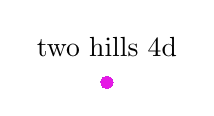
\begin{tikzpicture}

% defining custom colors
\definecolor{mycolor1}{rgb}{1,0.1,0.1}
\definecolor{mycolor2}{rgb}{0.1,1,0.1}
\definecolor{mycolor3}{rgb}{0.1,0.1,1}
\definecolor{mycolor4}{rgb}{0.1,1,1}
\definecolor{mycolor5}{rgb}{0.9,0.1,0.9}


\begin{axis}[%
view={-72}{42},
xmin=0, xmax=100,
xlabel={Number of samples},
xmajorgrids,
y dir=reverse,
ymin=-40, ymax=40,
ylabel={sample location},
ymajorgrids,
zmin=0, zmax=0.04,
zmajorgrids,
axis lines=left,
scale only axis,
width=\fwidth,
height=\fheight,
title={two hills 4d}]
\addplot3 [
color=mycolor1,
only marks,
mark=*,
mark options={solid}
]
coordinates{
 (1,8.64397318249258,0)(2,0.94202610858281,0)(3,-8.51909224508774,0)(4,8.73504449150106,0)(5,-4.38039043088074,0)(6,-4.29661051911298,0)(7,-11.0272856023819,0)(8,3.9624682112797,0)(9,-9.64925101622627,0)(10,1.68448763331274,0)(11,-19.6535886818246,0)(12,-7.44302088643632,0)(13,-5.52306700484431,0)(14,-8.19726048957947,0)(15,11.0914180018547,0)(16,-6.14945861779946,0)(17,-2.54635294228131,0)(18,-2.6982964643979,0)(19,-16.7199406378983,0)(20,-18.7604530491713,0)(21,5.75006015878006,0)(22,-8.66133150431014,0)(23,-21.1652270104548,0)(24,-9.64465668893709,0)(25,2.12729440847614,0)(26,4.77917410863812,0)(27,1.0065773429252,0)(28,2.97433365310199,0)(29,5.70148492190659,0)(30,-16.2449561946395,0)(31,6.43442896614198,0)(32,6.81861101501212,0)(33,0.146545462976063,0)(34,-13.0154083556885,0)(35,-12.8458694199502,0)(36,8.12213221007246,0)(37,8.38548117504491,0)(38,14.2032099924033,0)(39,-9.89751963936141,0)(40,-11.8322927670026,0)(41,-4.66258701033501,0)(42,-3.65943456601606,0)(43,11.1833282594471,0)(44,-4.65614764979949,0)(45,-15.6079951442098,0)(46,-2.83103049634655,0)(47,-13.2294142478163,0)(48,-1.96238020663121,0)(49,4.19039092209372,0)(50,7.42318242363705,0)(51,-1.43031901660663,0)(52,-21.6194345485188,0)(53,-6.44226188013935,0)(54,14.3958966362552,0)(55,-8.46916703704845,0)(56,0.573396598842837,0)(57,6.43407819310009,0)(58,-6.70431031039433,0)(59,-0.0314182038723435,0)(60,3.5293137585827,0)(61,11.7950226794027,0)(62,-6.85902078686398,0)(63,16.7678943259546,0)(64,-2.55308776295612,0)(65,-6.47548492231093,0)(66,-1.82214217198884,0)(67,8.51800292262651,0)(68,-3.06550037434344,0)(69,-4.40528888444301,0)(70,-6.11471876975789,0)(71,-4.85206910127117,0)(72,11.9701928905678,0)(73,13.9478769033299,0)(74,1.65367561474691,0)(75,-5.09966956368727,0)(76,13.7771664896642,0)(77,12.9851755410422,0)(78,-1.30117041997769,0)(79,7.40248586252175,0)(80,13.320174467912,0)(81,-2.78070689182663,0)(82,-3.27992902252155,0)(83,-0.125272443409905,0)(84,9.03178709204238,0)(85,-11.1246332865596,0)(86,-8.39210796544983,0)(87,0.355343920326862,0)(88,-12.4652893677206,0)(89,8.84505037335452,0)(90,25.3833384421976,0)(91,13.1679503886664,0)(92,14.4221307180034,0)(93,14.6691939938362,0)(94,-11.0705180813558,0)(95,-4.60936138301192,0)(96,-0.202959162388906,0)(97,-0.459981798696434,0)(98,-5.44486576241684,0)(99,9.17034563222667,0)(100,-0.194183076797647,0) 
};

\addplot3 [
color=mycolor2,
only marks,
mark=*,
mark options={solid}
]
coordinates{
 (1,7.25877210225363,0)(2,7.25877210225363,0)(3,5.5122249617504,0)(4,4.70699745932238,0)(5,4.70699745932238,0)(6,5.3797070177749,0)(7,7.18267485760811,0)(8,7.18267485760811,0)(9,9.83439683656881,0)(10,8.35995736243145,0)(11,3.42427592597632,0)(12,3.42427592597632,0)(13,1.38705384352442,0)(14,1.38705384352442,0)(15,5.11696751554988,0)(16,3.06923938469177,0)(17,1.67616472210555,0)(18,1.67616472210555,0)(19,1.67616472210555,0)(20,0.796827993755592,0)(21,-2.7210899382097,0)(22,-2.7210899382097,0)(23,-2.7210899382097,0)(24,-2.86654895481988,0)(25,-2.86654895481988,0)(26,-2.86654895481988,0)(27,-7.87597180805479,0)(28,-12.7209444587649,0)(29,-11.8622781257905,0)(30,-11.8622781257905,0)(31,-13.2152312870819,0)(32,-13.2152312870819,0)(33,-13.2152312870819,0)(34,-13.2152312870819,0)(35,-13.2152312870819,0)(36,-14.9918851020262,0)(37,-14.7299549914729,0)(38,-14.7299549914729,0)(39,-14.7299549914729,0)(40,-14.7299549914729,0)(41,-14.7299549914729,0)(42,-14.7299549914729,0)(43,-14.7299549914729,0)(44,-14.7299549914729,0)(45,-14.8690279250911,0)(46,-14.8690279250911,0)(47,-14.8690279250911,0)(48,-14.8690279250911,0)(49,-14.8690279250911,0)(50,-14.8690279250911,0)(51,-12.1537199135851,0)(52,-12.1537199135851,0)(53,-10.7565337123758,0)(54,-12.4881629189951,0)(55,-12.4881629189951,0)(56,-12.4881629189951,0)(57,-12.4881629189951,0)(58,-10.8422792459222,0)(59,-10.8422792459222,0)(60,-10.8422792459222,0)(61,-10.8422792459222,0)(62,-10.8422792459222,0)(63,-10.8422792459222,0)(64,-10.8422792459222,0)(65,-8.09932913118103,0)(66,-2.42231930817771,0)(67,-2.42231930817771,0)(68,-2.42231930817771,0)(69,-9.5767622129988,0)(70,-9.5767622129988,0)(71,-9.5767622129988,0)(72,-7.23335783733829,0)(73,-7.23335783733829,0)(74,-7.23335783733829,0)(75,-7.23335783733829,0)(76,-7.23335783733829,0)(77,-4.53361513103103,0)(78,-4.53361513103103,0)(79,-4.53361513103103,0)(80,-4.53361513103103,0)(81,-4.53361513103103,0)(82,-4.53361513103103,0)(83,-4.53361513103103,0)(84,-4.53361513103103,0)(85,-4.53361513103103,0)(86,-4.53361513103103,0)(87,-4.53361513103103,0)(88,-4.53361513103103,0)(89,-4.53361513103103,0)(90,-4.53361513103103,0)(91,-4.53361513103103,0)(92,-4.53361513103103,0)(93,-4.29099355258858,0)(94,-4.29099355258858,0)(95,-4.29099355258858,0)(96,-4.29099355258858,0)(97,-4.29099355258858,0)(98,-4.29099355258858,0)(99,-10.1713797999397,0)(100,-10.1713797999397,0) 
};

\addplot3 [
color=mycolor3,
only marks,
mark=*,
mark options={solid}
]
coordinates{
 (1,7.25877210225363,0)(2,7.25877210225363,0)(3,5.5122249617504,0)(4,4.70699745932238,0)(5,4.70699745932238,0)(6,5.3797070177749,0)(7,7.18267485760811,0)(8,7.18267485760811,0)(9,9.83439683656881,0)(10,8.35995736243145,0)(11,3.42427592597632,0)(12,3.42427592597632,0)(13,1.38705384352442,0)(14,1.38705384352442,0)(15,5.11696751554988,0)(16,3.06923938469177,0)(17,1.67616472210555,0)(18,1.67616472210555,0)(19,1.67616472210555,0)(20,0.796827993755592,0)(21,-2.7210899382097,0)(22,-2.7210899382097,0)(23,-2.7210899382097,0)(24,-2.86654895481988,0)(25,-2.86654895481988,0)(26,-2.86654895481988,0)(27,-7.87597180805479,0)(28,-12.7209444587649,0)(29,-11.8622781257905,0)(30,-11.8622781257905,0)(31,-13.2152312870819,0)(32,-13.2152312870819,0)(33,-13.2152312870819,0)(34,-13.2152312870819,0)(35,-13.2152312870819,0)(36,-14.9918851020262,0)(37,-14.7299549914729,0)(38,-14.7299549914729,0)(39,-14.7299549914729,0)(40,-14.7299549914729,0)(41,-14.7299549914729,0)(42,-14.7299549914729,0)(43,-14.7299549914729,0)(44,-14.7299549914729,0)(45,-14.8690279250911,0)(46,-14.8690279250911,0)(47,-14.8690279250911,0)(48,-14.8690279250911,0)(49,-14.8690279250911,0)(50,-14.8690279250911,0)(51,-12.1537199135851,0)(52,-12.1537199135851,0)(53,-10.7565337123758,0)(54,-12.4881629189951,0)(55,-12.4881629189951,0)(56,-12.4881629189951,0)(57,-12.4881629189951,0)(58,-10.8422792459222,0)(59,-10.8422792459222,0)(60,-10.8422792459222,0)(61,-10.8422792459222,0)(62,-10.8422792459222,0)(63,-10.8422792459222,0)(64,-10.8422792459222,0)(65,-8.09932913118103,0)(66,-2.42231930817771,0)(67,-2.42231930817771,0)(68,-2.42231930817771,0)(69,-9.5767622129988,0)(70,-9.5767622129988,0)(71,-9.5767622129988,0)(72,-7.23335783733829,0)(73,-7.23335783733829,0)(74,-7.23335783733829,0)(75,-7.23335783733829,0)(76,-7.23335783733829,0)(77,-4.53361513103103,0)(78,-4.53361513103103,0)(79,-4.53361513103103,0)(80,-4.53361513103103,0)(81,-4.53361513103103,0)(82,-4.53361513103103,0)(83,-4.53361513103103,0)(84,-4.53361513103103,0)(85,-4.53361513103103,0)(86,-4.53361513103103,0)(87,-4.53361513103103,0)(88,-4.53361513103103,0)(89,-4.53361513103103,0)(90,-4.53361513103103,0)(91,-4.53361513103103,0)(92,-4.53361513103103,0)(93,-4.29099355258858,0)(94,-4.29099355258858,0)(95,-4.29099355258858,0)(96,-4.29099355258858,0)(97,-4.29099355258858,0)(98,-4.29099355258858,0)(99,-10.1713797999397,0)(100,-10.1713797999397,0) 
};

\addplot3 [
color=mycolor4,
only marks,
mark=*,
mark options={solid}
]
coordinates{
 (1,8.64397318249258,0)(2,-4.38039043088074,0)(3,-9.64925101622627,0)(4,-5.52306700484431,0)(5,-2.54635294228131,0)(6,5.75006015878006,0)(7,2.12729440847614,0)(8,5.70148492190659,0)(9,0.146545462976063,0)(10,8.38548117504491,0)(11,-4.66258701033501,0)(12,-15.6079951442098,0)(13,4.19039092209372,0)(14,-6.44226188013935,0)(15,6.43407819310009,0)(16,11.7950226794027,0)(17,-6.47548492231093,0)(18,-4.40528888444301,0)(19,13.9478769033299,0)(20,12.9851755410422,0)(21,-2.78070689182663,0)(22,-11.1246332865596,0)(23,8.84505037335452,0)(24,14.6691939938362,0)(25,-0.459981798696434,0)(26,7.74630170067919,0)(27,6.8593778037851,0)(28,-15.8411859791217,0)(29,-15.3211487774673,0)(30,2.71534136230341,0)(31,-5.50556055505238,0)(32,-4.27841355720601,0)(33,-12.8432806164091,0)(34,22.788714924349,0)(35,-8.33888222877994,0)(36,-9.25689568236607,0)(37,-5.61827266885125,0)(38,0.828295737128377,0)(39,-0.910346091729716,0)(40,-9.28710447028532,0)(41,0,0)(42,-9.41710232692403,0)(43,16.2075129330797,0)(44,-6.35514086344284,0)(45,-20.4726855027881,0)(46,-0.87972504507333,0)(47,-0.439787231114959,0)(48,-2.14829528926237,0)(49,-7.46695232460116,0)(50,10.0346920730319,0)(51,1.06501925298886,0)(52,-10.8651159936796,0)(53,8.58655786526147,0)(54,-3.26146433447351,0)(55,4.41829071117974,0)(56,-5.47589235578721,0)(57,-16.4297445292357,0)(58,-2.51608297481982,0)(59,-0.386248047719412,0)(60,5.20474117059437,0)(61,11.5973134212842,0)(62,-15.3281983976842,0)(63,-13.9051466783837,0)(64,3.45155795737528,0)(65,-0.480373835359512,0)(66,0.571314603916797,0)(67,8.67396987080217,0)(68,17.9522813398399,0)(69,5.22442218786417,0)(70,-5.43988057630887,0)(71,-22.6243349688659,0)(72,-0.155033585159644,0)(73,-7.30090998573805,0)(74,7.41049530589206,0)(75,15.0507321352726,0)(76,-12.7806691875923,0)(77,-4.98405983066428,0)(78,9.86615924967321,0)(79,8.53733604835799,0)(80,-1.91396023802537,0)(81,-9.65133704029641,0)(82,20.1838052497679,0)(83,-7.26842720767158,0)(84,-8.67937826619676,0)(85,4.85959542900476,0)(86,-14.8766922867241,0)(87,-11.0750411220868,0)(88,-9.18766881909361,0)(89,-7.62727133228085,0)(90,-8.55062699296247,0)(91,-6.32951970568829,0)(92,17.790376880496,0)(93,-0.235713608468783,0)(94,-5.40453938066577,0)(95,0.767236797383346,0)(96,7.55429908599643,0)(97,-13.8998730188666,0)(98,23.7101392186287,0)(99,-4.1303280502124,0)(100,15.0075011042154,0) 
};

\addplot3 [
color=mycolor5,
only marks,
mark=*,
mark options={solid}
]
coordinates{
 (1,7.25877210225363,0)(2,7.25877210225363,0)(3,5.5122249617504,0)(4,4.70699745932238,0)(5,4.70699745932238,0)(6,5.3797070177749,0)(7,7.18267485760811,0)(8,7.18267485760811,0)(9,9.83439683656881,0)(10,8.35995736243145,0)(11,3.42427592597632,0)(12,3.42427592597632,0)(13,1.38705384352442,0)(14,1.38705384352442,0)(15,5.11696751554988,0)(16,3.06923938469177,0)(17,1.67616472210555,0)(18,1.67616472210555,0)(19,1.67616472210555,0)(20,0.796827993755592,0)(21,-2.7210899382097,0)(22,-2.7210899382097,0)(23,-2.7210899382097,0)(24,-2.86654895481988,0)(25,-2.86654895481988,0)(26,-2.86654895481988,0)(27,-7.87597180805479,0)(28,-12.7209444587649,0)(29,-11.8622781257905,0)(30,-11.8622781257905,0)(31,-13.2152312870819,0)(32,-13.2152312870819,0)(33,-13.2152312870819,0)(34,-13.2152312870819,0)(35,-13.2152312870819,0)(36,-14.9918851020262,0)(37,-14.7299549914729,0)(38,-14.7299549914729,0)(39,-14.7299549914729,0)(40,-14.7299549914729,0)(41,-14.7299549914729,0)(42,-14.7299549914729,0)(43,-14.7299549914729,0)(44,-14.7299549914729,0)(45,-14.8690279250911,0)(46,-14.8690279250911,0)(47,-14.8690279250911,0)(48,-14.8690279250911,0)(49,-14.8690279250911,0)(50,-14.8690279250911,0)(51,-12.1537199135851,0)(52,-12.1537199135851,0)(53,-10.7565337123758,0)(54,-12.4881629189951,0)(55,-12.4881629189951,0)(56,-12.4881629189951,0)(57,-12.4881629189951,0)(58,-10.8422792459222,0)(59,-10.8422792459222,0)(60,-10.8422792459222,0)(61,-10.8422792459222,0)(62,-10.8422792459222,0)(63,-10.8422792459222,0)(64,-10.8422792459222,0)(65,-8.09932913118103,0)(66,-2.42231930817771,0)(67,-2.42231930817771,0)(68,-2.42231930817771,0)(69,-9.5767622129988,0)(70,-9.5767622129988,0)(71,-9.5767622129988,0)(72,-7.23335783733829,0)(73,-7.23335783733829,0)(74,-7.23335783733829,0)(75,-7.23335783733829,0)(76,-7.23335783733829,0)(77,-4.53361513103103,0)(78,-4.53361513103103,0)(79,-4.53361513103103,0)(80,-4.53361513103103,0)(81,-4.53361513103103,0)(82,-4.53361513103103,0)(83,-4.53361513103103,0)(84,-4.53361513103103,0)(85,-4.53361513103103,0)(86,-4.53361513103103,0)(87,-4.53361513103103,0)(88,-4.53361513103103,0)(89,-4.53361513103103,0)(90,-4.53361513103103,0)(91,-4.53361513103103,0)(92,-4.53361513103103,0)(93,-4.29099355258858,0)(94,-4.29099355258858,0)(95,-4.29099355258858,0)(96,-4.29099355258858,0)(97,-4.29099355258858,0)(98,-4.29099355258858,0)(99,-10.1713797999397,0)(100,-10.1713797999397,0) 
};

\addplot3 [
color=black,
solid,
line width=2.0pt
]
coordinates{
 (101,-40,1.33830225764885e-05)(101,-39.9199199199199,1.38182046410497e-05)(101,-39.8398398398398,1.42666228042307e-05)(101,-39.7597597597598,1.47286481503254e-05)(101,-39.6796796796797,1.52046611333821e-05)(101,-39.5995995995996,1.56950517814782e-05)(101,-39.5195195195195,1.6200219904485e-05)(101,-39.4394394394394,1.6720575305353e-05)(101,-39.3593593593594,1.72565379949497e-05)(101,-39.2792792792793,1.7808538410479e-05)(101,-39.1991991991992,1.83770176375138e-05)(101,-39.1191191191191,1.89624276356684e-05)(101,-39.039039039039,1.95652314679408e-05)(101,-38.958958958959,2.01859035337517e-05)(101,-38.8788788788789,2.08249298057069e-05)(101,-38.7987987987988,2.14828080701089e-05)(101,-38.7187187187187,2.21600481712426e-05)(101,-38.6386386386386,2.285717225946e-05)(101,-38.5585585585586,2.35747150430845e-05)(101,-38.4784784784785,2.43132240441603e-05)(101,-38.3983983983984,2.50732598580649e-05)(101,-38.3183183183183,2.58553964170059e-05)(101,-38.2382382382382,2.66602212574213e-05)(101,-38.1581581581582,2.74883357912987e-05)(101,-38.0780780780781,2.83403555814326e-05)(101,-37.997997997998,2.92169106206323e-05)(101,-37.9179179179179,3.01186456148956e-05)(101,-37.8378378378378,3.104622027056e-05)(101,-37.7577577577578,3.20003095854415e-05)(101,-37.6776776776777,3.29816041439723e-05)(101,-37.5975975975976,3.39908104163431e-05)(101,-37.5175175175175,3.50286510616579e-05)(101,-37.4374374374374,3.60958652351047e-05)(101,-37.3573573573574,3.71932088991451e-05)(101,-37.2772772772773,3.8321455138726e-05)(101,-37.1971971971972,3.94813944805093e-05)(101,-37.1171171171171,4.06738352161196e-05)(101,-37.037037037037,4.18996037294058e-05)(101,-36.956956956957,4.31595448277079e-05)(101,-36.8768768768769,4.4454522077123e-05)(101,-36.7967967967968,4.57854181417587e-05)(101,-36.7167167167167,4.71531351269623e-05)(101,-36.6366366366366,4.85585949265103e-05)(101,-36.5565565565566,5.00027395737409e-05)(101,-36.4764764764765,5.14865315966113e-05)(101,-36.3963963963964,5.30109543766577e-05)(101,-36.3163163163163,5.45770125118335e-05)(101,-36.2362362362362,5.61857321831992e-05)(101,-36.1561561561562,5.78381615254348e-05)(101,-36.0760760760761,5.95353710011453e-05)(101,-35.995995995996,6.12784537789192e-05)(101,-35.9159159159159,6.30685261151104e-05)(101,-35.8358358358358,6.49067277392972e-05)(101,-35.7557557557558,6.67942222433795e-05)(101,-35.6756756756757,6.87321974742665e-05)(101,-35.5955955955956,7.07218659301082e-05)(101,-35.5155155155155,7.27644651600165e-05)(101,-35.4354354354354,7.48612581672246e-05)(101,-35.3553553553554,7.70135338156225e-05)(101,-35.2752752752753,7.9222607239612e-05)(101,-35.1951951951952,8.1489820257214e-05)(101,-35.1151151151151,8.38165417863602e-05)(101,-35.035035035035,8.62041682643007e-05)(101,-34.954954954955,8.86541240700501e-05)(101,-34.8748748748749,9.11678619497959e-05)(101,-34.7947947947948,9.37468634451866e-05)(101,-34.7147147147147,9.63926393244148e-05)(101,-34.6346346346346,9.91067300160058e-05)(101,-34.5545545545546,0.00010189070604522)(101,-34.4744744744745,0.000104746168472971)(101,-34.3943943943944,0.00010767474933716)(101,-34.3143143143143,0.000110678112096323)(101,-34.2342342342342,0.000113757952075483)(101,-34.1541541541542,0.000116915996914087)(101,-34.0740740740741,0.000120154007015926)(101,-33.993993993994,0.000123473776000907)(101,-33.9139139139139,0.000126877131158549)(101,-33.8338338338338,0.000130365933903088)(101,-33.7537537537538,0.000133942080230046)(101,-33.6736736736737,0.000137607501174126)(101,-33.5935935935936,0.0001413641632683)(101,-33.5135135135135,0.000145214069003937)(101,-33.4334334334334,0.00014915925729182)(101,-33.3533533533534,0.000153201803923895)(101,-33.2732732732733,0.000157343822035606)(101,-33.1931931931932,0.000161587462568624)(101,-33.1131131131131,0.000165934914733831)(101,-33.033033033033,0.000170388406474362)(101,-32.952952952953,0.000174950204928538)(101,-32.8728728728729,0.000179622616892505)(101,-32.7927927927928,0.000184407989282385)(101,-32.7127127127127,0.000189308709595757)(101,-32.6326326326326,0.000194327206372254)(101,-32.5525525525526,0.000199465949653091)(101,-32.4724724724725,0.000204727451439301)(101,-32.3923923923924,0.000210114266148476)(101,-32.3123123123123,0.000215628991069791)(101,-32.2322322322322,0.000221274266817093)(101,-32.1521521521522,0.000227052777779814)(101,-32.0720720720721,0.000232967252571501)(101,-31.991991991992,0.000239020464475689)(101,-31.9119119119119,0.000245215231888918)(101,-31.8318318318318,0.000251554418760605)(101,-31.7517517517518,0.000258040935029545)(101,-31.6716716716717,0.000264677737056775)(101,-31.5915915915916,0.000271467828054534)(101,-31.5115115115115,0.000278414258511061)(101,-31.4314314314314,0.000285520126610952)(101,-31.3513513513514,0.000292788578650791)(101,-31.2712712712713,0.000300222809449793)(101,-31.1911911911912,0.000307826062755151)(101,-31.1111111111111,0.000315601631641804)(101,-31.031031031031,0.000323552858906328)(101,-30.950950950951,0.000331683137454643)(101,-30.8708708708709,0.000339995910683238)(101,-30.7907907907908,0.000348494672853595)(101,-30.7107107107107,0.000357182969459489)(101,-30.6306306306306,0.000366064397586863)(101,-30.5505505505506,0.000375142606265932)(101,-30.4704704704705,0.000384421296815189)(101,-30.3903903903904,0.000393904223176991)(101,-30.3103103103103,0.000403595192244368)(101,-30.2302302302302,0.000413498064178719)(101,-30.1501501501502,0.000423616752718052)(101,-30.0700700700701,0.000433955225475398)(101,-29.98998998999,0.000444517504227068)(101,-29.9099099099099,0.000455307665190355)(101,-29.8298298298298,0.000466329839290368)(101,-29.7497497497497,0.000477588212415564)(101,-29.6696696696697,0.000489087025661667)(101,-29.5895895895896,0.000500830575563558)(101,-29.5095095095095,0.000512823214314763)(101,-29.4294294294294,0.000525069349974172)(101,-29.3493493493493,0.000537573446659573)(101,-29.2692692692693,0.000550340024727644)(101,-29.1891891891892,0.000563373660939975)(101,-29.1091091091091,0.00057667898861475)(101,-29.029029029029,0.000590260697763673)(101,-28.9489489489489,0.000604123535213746)(101,-28.8688688688689,0.000618272304713484)(101,-28.7887887887888,0.000632711867023164)(101,-28.7087087087087,0.000647447139988702)(101,-28.6286286286286,0.000662483098598742)(101,-28.5485485485485,0.000677824775024529)(101,-28.4684684684685,0.00069347725864219)(101,-28.3883883883884,0.000709445696036946)(101,-28.3083083083083,0.000725735290988892)(101,-28.2282282282282,0.000742351304439893)(101,-28.1481481481481,0.000759299054441176)(101,-28.0680680680681,0.00077658391608121)(101,-27.987987987988,0.000794211321393438)(101,-27.9079079079079,0.000812186759243431)(101,-27.8278278278278,0.000830515775195072)(101,-27.7477477477477,0.000849203971355292)(101,-27.6676676676677,0.000868257006197)(101,-27.5875875875876,0.000887680594359711)(101,-27.5075075075075,0.00090748050642751)(101,-27.4274274274274,0.000927662568683897)(101,-27.3473473473473,0.0009482326628431)(101,-27.2672672672673,0.000969196725757424)(101,-27.1871871871872,0.000990560749100247)(101,-27.1071071071071,0.00101233077902421)(101,-27.027027027027,0.00103451291579421)(101,-26.9469469469469,0.00105711331339476)(101,-26.8668668668669,0.00108013817911136)(101,-26.7867867867868,0.0011035937730854)(101,-26.7067067067067,0.00112748640784219)(101,-26.6266266266266,0.00115182244779185)(101,-26.5465465465465,0.00117660830870247)(101,-26.4664664664665,0.00120185045714527)(101,-26.3863863863864,0.00122755540991133)(101,-26.3063063063063,0.00125372973339956)(101,-26.2262262262262,0.00128038004297541)(101,-26.1461461461461,0.00130751300230007)(101,-26.0660660660661,0.00133513532262973)(101,-25.985985985986,0.00136325376208454)(101,-25.9059059059059,0.00139187512488693)(101,-25.8258258258258,0.0014210062605689)(101,-25.7457457457457,0.00145065406314803)(101,-25.6656656656657,0.00148082547027168)(101,-25.5855855855856,0.00151152746232934)(101,-25.5055055055055,0.00154276706153247)(101,-25.4254254254254,0.00157455133096184)(101,-25.3453453453453,0.00160688737358179)(101,-25.2652652652653,0.0016397823312213)(101,-25.1851851851852,0.00167324338352152)(101,-25.1051051051051,0.00170727774684939)(101,-25.025025025025,0.00174189267317727)(101,-24.9449449449449,0.00177709544892815)(101,-24.8648648648649,0.00181289339378627)(101,-24.7847847847848,0.00184929385947285)(101,-24.7047047047047,0.00188630422848682)(101,-24.6246246246246,0.00192393191281025)(101,-24.5445445445445,0.00196218435257817)(101,-24.4644644644645,0.00200106901471285)(101,-24.3843843843844,0.0020405933915221)(101,-24.3043043043043,0.0020807649992616)(101,-24.2242242242242,0.00212159137666093)(101,-24.1441441441441,0.00216308008341344)(101,-24.0640640640641,0.00220523869862944)(101,-23.983983983984,0.00224807481925294)(101,-23.9039039039039,0.0022915960584417)(101,-23.8238238238238,0.00233581004391047)(101,-23.7437437437437,0.0023807244162374)(101,-23.6636636636637,0.00242634682713357)(101,-23.5835835835836,0.00247268493767558)(101,-23.5035035035035,0.00251974641650119)(101,-23.4234234234234,0.00256753893796796)(101,-23.3433433433433,0.00261607018027502)(101,-23.2632632632633,0.00266534782354776)(101,-23.1831831831832,0.00271537954788581)(101,-23.1031031031031,0.00276617303137407)(101,-23.023023023023,0.00281773594805703)(101,-22.9429429429429,0.00287007596587648)(101,-22.8628628628629,0.00292320074457259)(101,-22.7827827827828,0.0029771179335487)(101,-22.7027027027027,0.00303183516969979)(101,-22.6226226226226,0.00308736007520491)(101,-22.5425425425425,0.00314370025528369)(101,-22.4624624624625,0.00320086329591723)(101,-22.3823823823824,0.00325885676153351)(101,-22.3023023023023,0.00331768819265761)(101,-22.2222222222222,0.00337736510352706)(101,-22.1421421421421,0.00343789497967251)(101,-22.0620620620621,0.00349928527546413)(101,-21.981981981982,0.00356154341162401)(101,-21.9019019019019,0.00362467677270497)(101,-21.8218218218218,0.00368869270453615)(101,-21.7417417417417,0.00375359851163568)(101,-21.6616616616617,0.00381940145459099)(101,-21.5815815815816,0.00388610874740723)(101,-21.5015015015015,0.00395372755482399)(101,-21.4214214214214,0.0040222649896012)(101,-21.3413413413413,0.00409172810977437)(101,-21.2612612612613,0.00416212391588003)(101,-21.1811811811812,0.00423345934815158)(101,-21.1011011011011,0.00430574128368641)(101,-21.021021021021,0.00437897653358481)(101,-20.9409409409409,0.00445317184006117)(101,-20.8608608608609,0.00452833387352837)(101,-20.7807807807808,0.00460446922965576)(101,-20.7007007007007,0.00468158442640166)(101,-20.6206206206206,0.00475968590102091)(101,-20.5405405405405,0.00483878000704834)(101,-20.4604604604605,0.00491887301125894)(101,-20.3803803803804,0.00499997109060533)(101,-20.3003003003003,0.00508208032913362)(101,-20.2202202202202,0.00516520671487824)(101,-20.1401401401401,0.00524935613673682)(101,-20.0600600600601,0.0053345343813258)(101,-19.97997997998,0.00542074712981784)(101,-19.8998998998999,0.00550799995476186)(101,-19.8198198198198,0.00559629831688667)(101,-19.7397397397397,0.00568564756188931)(101,-19.6596596596597,0.00577605291720876)(101,-19.5795795795796,0.0058675194887865)(101,-19.4994994994995,0.00596005225781458)(101,-19.4194194194194,0.00605365607747232)(101,-19.3393393393393,0.0061483356696531)(101,-19.2592592592593,0.0062440956216817)(101,-19.1791791791792,0.00634094038302401)(101,-19.0990990990991,0.00643887426198963)(101,-19.019019019019,0.00653790142242912)(101,-18.9389389389389,0.00663802588042656)(101,-18.8588588588589,0.00673925150098903)(101,-18.7787787787788,0.00684158199473404)(101,-18.6986986986987,0.00694502091457626)(101,-18.6186186186186,0.00704957165241465)(101,-18.5385385385385,0.00715523743582165)(101,-18.4584584584585,0.00726202132473521)(101,-18.3783783783784,0.00736992620815557)(101,-18.2982982982983,0.00747895480084762)(101,-18.2182182182182,0.00758910964005057)(101,-18.1381381381381,0.00770039308219614)(101,-18.0580580580581,0.00781280729963669)(101,-17.977977977978,0.00792635427738473)(101,-17.8978978978979,0.00804103580986525)(101,-17.8178178178178,0.00815685349768226)(101,-17.7377377377377,0.00827380874440108)(101,-17.6576576576577,0.00839190275334777)(101,-17.5775775775776,0.00851113652442723)(101,-17.4974974974975,0.0086315108509615)(101,-17.4174174174174,0.00875302631654975)(101,-17.3373373373373,0.00887568329195139)(101,-17.2572572572573,0.00899948193199405)(101,-17.1771771771772,0.00912442217250772)(101,-17.0970970970971,0.00925050372728685)(101,-17.017017017017,0.00937772608508176)(101,-16.9369369369369,0.00950608850662112)(101,-16.8568568568569,0.00963559002166691)(101,-16.7767767767768,0.00976622942610364)(101,-16.6966966966967,0.0098980052790632)(101,-16.6166166166166,0.0100309159000872)(101,-16.5365365365365,0.0101649593663279)(101,-16.4564564564565,0.0103001335097907)(101,-16.3763763763764,0.010436435914617)(101,-16.2962962962963,0.0105738639144131)(101,-16.2162162162162,0.0107124145896225)(101,-16.1361361361361,0.0108520847649465)(101,-16.0560560560561,0.010992871006813)(101,-15.975975975976,0.0111347696208955)(101,-15.8958958958959,0.0112777766496842)(101,-15.8158158158158,0.0114218878701105)(101,-15.7357357357357,0.0115670987912262)(101,-15.6556556556557,0.0117134046519405)(101,-15.5755755755756,0.011860800418814)(101,-15.4954954954955,0.0120092807839133)(101,-15.4154154154154,0.0121588401627275)(101,-15.3353353353353,0.0123094726921466)(101,-15.2552552552553,0.0124611722285057)(101,-15.1751751751752,0.012613932345695)(101,-15.0950950950951,0.0127677463333369)(101,-15.015015015015,0.0129226071950339)(101,-14.9349349349349,0.0130785076466857)(101,-14.8548548548549,0.0132354401148798)(101,-14.7747747747748,0.0133933967353555)(101,-14.6946946946947,0.013552369351543)(101,-14.6146146146146,0.0137123495131801)(101,-14.5345345345345,0.013873328475006)(101,-14.4544544544545,0.0140352971955359)(101,-14.3743743743744,0.0141982463359159)(101,-14.2942942942943,0.0143621662588612)(101,-14.2142142142142,0.014527047027677)(101,-14.1341341341341,0.0146928784053658)(101,-14.0540540540541,0.0148596498538208)(101,-13.973973973974,0.0150273505331067)(101,-13.8938938938939,0.0151959693008306)(101,-13.8138138138138,0.0153654947116025)(101,-13.7337337337337,0.0155359150165875)(101,-13.6536536536537,0.0157072181631514)(101,-13.5735735735736,0.0158793917945997)(101,-13.4934934934935,0.0160524232500122)(101,-13.4134134134134,0.016226299564173)(101,-13.3333333333333,0.0164010074675994)(101,-13.2532532532533,0.0165765333866673)(101,-13.1731731731732,0.0167528634438376)(101,-13.0930930930931,0.0169299834579821)(101,-13.013013013013,0.017107878944811)(101,-12.9329329329329,0.0172865351174024)(101,-12.8528528528529,0.0174659368868355)(101,-12.7727727727728,0.0176460688629273)(101,-12.6926926926927,0.0178269153550739)(101,-12.6126126126126,0.018008460373198)(101,-12.5325325325325,0.0181906876288021)(101,-12.4524524524525,0.0183735805361283)(101,-12.3723723723724,0.0185571222134271)(101,-12.2922922922923,0.0187412954843324)(101,-12.2122122122122,0.018926082879347)(101,-12.1321321321321,0.0191114666374361)(101,-12.0520520520521,0.0192974287077311)(101,-11.971971971972,0.0194839507513435)(101,-11.8918918918919,0.019671014143289)(101,-11.8118118118118,0.0198585999745227)(101,-11.7317317317317,0.0200466890540856)(101,-11.6516516516517,0.0202352619113618)(101,-11.5715715715716,0.0204242987984477)(101,-11.4914914914915,0.0206137796926331)(101,-11.4114114114114,0.0208036842989938)(101,-11.3313313313313,0.0209939920530956)(101,-11.2512512512513,0.021184682123811)(101,-11.1711711711712,0.021375733416247)(101,-11.0910910910911,0.0215671245747847)(101,-11.011011011011,0.0217588339862305)(101,-10.9309309309309,0.0219508397830784)(101,-10.8508508508509,0.0221431198468836)(101,-10.7707707707708,0.0223356518117463)(101,-10.6906906906907,0.0225284130679063)(101,-10.6106106106106,0.022721380765447)(101,-10.5305305305305,0.0229145318181096)(101,-10.4504504504505,0.0231078429072154)(101,-10.3703703703704,0.0233012904856966)(101,-10.2902902902903,0.0234948507822352)(101,-10.2102102102102,0.0236884998055083)(101,-10.1301301301301,0.0238822133485401)(101,-10.0500500500501,0.024075966993159)(101,-9.96996996996997,0.0242697361145593)(101,-9.88988988988989,0.0244634958859672)(101,-9.80980980980981,0.0246572212834085)(101,-9.72972972972973,0.0248508870905785)(101,-9.64964964964965,0.025044467903813)(101,-9.56956956956957,0.0252379381371581)(101,-9.48948948948949,0.0254312720275384)(101,-9.40940940940941,0.0256244436400228)(101,-9.32932932932933,0.0258174268731856)(101,-9.24924924924925,0.0260101954645623)(101,-9.16916916916917,0.0262027229961987)(101,-9.08908908908909,0.0263949829002911)(101,-9.00900900900901,0.0265869484649171)(101,-8.92892892892893,0.0267785928398552)(101,-8.84884884884885,0.0269698890424904)(101,-8.76876876876877,0.0271608099638066)(101,-8.68868868868869,0.0273513283744617)(101,-8.60860860860861,0.0275414169309444)(101,-8.52852852852853,0.0277310481818124)(101,-8.44844844844845,0.0279201945740075)(101,-8.36836836836837,0.0281088284592474)(101,-8.28828828828829,0.028296922100493)(101,-8.20820820820821,0.0284844476784867)(101,-8.12812812812813,0.0286713772983616)(101,-8.04804804804805,0.0288576829963198)(101,-7.96796796796797,0.0290433367463758)(101,-7.88788788788789,0.0292283104671645)(101,-7.80780780780781,0.0294125760288111)(101,-7.72772772772772,0.0295961052598603)(101,-7.64764764764764,0.029778869954263)(101,-7.56756756756756,0.0299608418784177)(101,-7.48748748748748,0.0301419927782648)(101,-7.4074074074074,0.0303222943864308)(101,-7.32732732732732,0.0305017184294204)(101,-7.24724724724724,0.0306802366348536)(101,-7.16716716716716,0.0308578207387456)(101,-7.08708708708708,0.0310344424928268)(101,-7.007007007007,0.0312100736719007)(101,-6.92692692692692,0.0313846860812361)(101,-6.84684684684684,0.031558251563992)(101,-6.76676676676676,0.0317307420086723)(101,-6.68668668668668,0.0319021293566066)(101,-6.6066066066066,0.032072385609456)(101,-6.52652652652652,0.0322414828367396)(101,-6.44644644644644,0.0324093931833804)(101,-6.36636636636636,0.0325760888772662)(101,-6.28628628628628,0.0327415422368237)(101,-6.2062062062062,0.0329057256786028)(101,-6.12612612612612,0.0330686117248681)(101,-6.04604604604604,0.033230173011195)(101,-5.96596596596596,0.0333903822940662)(101,-5.88588588588588,0.0335492124584683)(101,-5.8058058058058,0.0337066365254824)(101,-5.72572572572572,0.0338626276598684)(101,-5.64564564564564,0.0340171591776383)(101,-5.56556556556556,0.0341702045536168)(101,-5.48548548548548,0.0343217374289848)(101,-5.4054054054054,0.0344717316188045)(101,-5.32532532532532,0.0346201611195215)(101,-5.24524524524524,0.0347670001164422)(101,-5.16516516516516,0.0349122229911825)(101,-5.08508508508508,0.0350558043290856)(101,-5.005005005005,0.0351977189266053)(101,-4.92492492492492,0.0353379417986526)(101,-4.84484484484484,0.0354764481859011)(101,-4.76476476476476,0.0356132135620502)(101,-4.68468468468468,0.0357482136410418)(101,-4.6046046046046,0.0358814243842273)(101,-4.52452452452452,0.0360128220074839)(101,-4.44444444444444,0.0361423829882743)(101,-4.36436436436436,0.0362700840726495)(101,-4.28428428428428,0.0363959022821904)(101,-4.2042042042042,0.0365198149208855)(101,-4.12412412412412,0.0366417995819425)(101,-4.04404404404404,0.03676183415453)(101,-3.96396396396396,0.0368798968304465)(101,-3.88388388388388,0.0369959661107154)(101,-3.8038038038038,0.037110020812101)(101,-3.72372372372372,0.0372220400735444)(101,-3.64364364364364,0.0373320033625156)(101,-3.56356356356356,0.0374398904812801)(101,-3.48348348348348,0.0375456815730761)(101,-3.4034034034034,0.0376493571282005)(101,-3.32332332332332,0.0377508979900006)(101,-3.24324324324324,0.0378502853607702)(101,-3.16316316316316,0.0379475008075448)(101,-3.08308308308308,0.0380425262677969)(101,-3.003003003003,0.0381353440550259)(101,-2.92292292292292,0.0382259368642425)(101,-2.84284284284284,0.038314287777343)(101,-2.76276276276276,0.0384003802683735)(101,-2.68268268268268,0.03848419820868)(101,-2.6026026026026,0.0385657258719425)(101,-2.52252252252252,0.0386449479390916)(101,-2.44244244244244,0.0387218495031049)(101,-2.36236236236236,0.0387964160736804)(101,-2.28228228228228,0.038868633581787)(101,-2.2022022022022,0.0389384883840873)(101,-2.12212212212212,0.0390059672672329)(101,-2.04204204204204,0.0390710574520297)(101,-1.96196196196196,0.0391337465974705)(101,-1.88188188188188,0.039194022804635)(101,-1.8018018018018,0.0392518746204527)(101,-1.72172172172172,0.0393072910413305)(101,-1.64164164164164,0.0393602615166401)(101,-1.56156156156156,0.0394107759520657)(101,-1.48148148148148,0.0394588247128102)(101,-1.4014014014014,0.0395043986266573)(101,-1.32132132132132,0.03954748898689)(101,-1.24124124124124,0.0395880875550626)(101,-1.16116116116116,0.0396261865636259)(101,-1.08108108108108,0.0396617787184037)(101,-1.001001001001,0.0396948572009207)(101,-0.920920920920921,0.0397254156705792)(101,-0.840840840840841,0.0397534482666846)(101,-0.76076076076076,0.039778949610319)(101,-0.68068068068068,0.039801914806061)(101,-0.6006006006006,0.0398223394435522)(101,-0.52052052052052,0.0398402195989086)(101,-0.44044044044044,0.0398555518359772)(101,-0.36036036036036,0.0398683332074364)(101,-0.28028028028028,0.0398785612557403)(101,-0.2002002002002,0.0398862340139061)(101,-0.12012012012012,0.0398913500061449)(101,-0.04004004004004,0.0398939082483343)(101,0.04004004004004,0.0398939082483343)(101,0.12012012012012,0.0398913500061449)(101,0.2002002002002,0.0398862340139061)(101,0.28028028028028,0.0398785612557403)(101,0.36036036036036,0.0398683332074364)(101,0.44044044044044,0.0398555518359772)(101,0.52052052052052,0.0398402195989086)(101,0.6006006006006,0.0398223394435522)(101,0.68068068068068,0.039801914806061)(101,0.76076076076076,0.039778949610319)(101,0.840840840840841,0.0397534482666846)(101,0.920920920920921,0.0397254156705792)(101,1.001001001001,0.0396948572009207)(101,1.08108108108108,0.0396617787184037)(101,1.16116116116116,0.0396261865636259)(101,1.24124124124124,0.0395880875550626)(101,1.32132132132132,0.03954748898689)(101,1.4014014014014,0.0395043986266573)(101,1.48148148148148,0.0394588247128102)(101,1.56156156156156,0.0394107759520657)(101,1.64164164164164,0.0393602615166401)(101,1.72172172172172,0.0393072910413305)(101,1.8018018018018,0.0392518746204527)(101,1.88188188188188,0.039194022804635)(101,1.96196196196196,0.0391337465974705)(101,2.04204204204204,0.0390710574520297)(101,2.12212212212212,0.0390059672672329)(101,2.2022022022022,0.0389384883840873)(101,2.28228228228228,0.038868633581787)(101,2.36236236236236,0.0387964160736804)(101,2.44244244244244,0.0387218495031049)(101,2.52252252252252,0.0386449479390916)(101,2.6026026026026,0.0385657258719425)(101,2.68268268268268,0.03848419820868)(101,2.76276276276276,0.0384003802683735)(101,2.84284284284284,0.038314287777343)(101,2.92292292292292,0.0382259368642425)(101,3.003003003003,0.0381353440550259)(101,3.08308308308308,0.0380425262677969)(101,3.16316316316316,0.0379475008075448)(101,3.24324324324324,0.0378502853607702)(101,3.32332332332332,0.0377508979900006)(101,3.4034034034034,0.0376493571282005)(101,3.48348348348348,0.0375456815730761)(101,3.56356356356356,0.0374398904812801)(101,3.64364364364364,0.0373320033625156)(101,3.72372372372372,0.0372220400735444)(101,3.8038038038038,0.037110020812101)(101,3.88388388388388,0.0369959661107154)(101,3.96396396396396,0.0368798968304465)(101,4.04404404404404,0.03676183415453)(101,4.12412412412412,0.0366417995819425)(101,4.2042042042042,0.0365198149208855)(101,4.28428428428428,0.0363959022821904)(101,4.36436436436436,0.0362700840726495)(101,4.44444444444444,0.0361423829882743)(101,4.52452452452452,0.0360128220074839)(101,4.6046046046046,0.0358814243842273)(101,4.68468468468468,0.0357482136410418)(101,4.76476476476476,0.0356132135620502)(101,4.84484484484484,0.0354764481859011)(101,4.92492492492492,0.0353379417986526)(101,5.005005005005,0.0351977189266053)(101,5.08508508508508,0.0350558043290856)(101,5.16516516516516,0.0349122229911825)(101,5.24524524524524,0.0347670001164422)(101,5.32532532532532,0.0346201611195215)(101,5.4054054054054,0.0344717316188045)(101,5.48548548548548,0.0343217374289848)(101,5.56556556556556,0.0341702045536168)(101,5.64564564564564,0.0340171591776383)(101,5.72572572572572,0.0338626276598684)(101,5.8058058058058,0.0337066365254824)(101,5.88588588588588,0.0335492124584683)(101,5.96596596596596,0.0333903822940662)(101,6.04604604604604,0.033230173011195)(101,6.12612612612612,0.0330686117248681)(101,6.2062062062062,0.0329057256786028)(101,6.28628628628628,0.0327415422368237)(101,6.36636636636636,0.0325760888772662)(101,6.44644644644644,0.0324093931833804)(101,6.52652652652652,0.0322414828367396)(101,6.6066066066066,0.032072385609456)(101,6.68668668668668,0.0319021293566066)(101,6.76676676676676,0.0317307420086723)(101,6.84684684684684,0.031558251563992)(101,6.92692692692692,0.0313846860812361)(101,7.007007007007,0.0312100736719007)(101,7.08708708708708,0.0310344424928268)(101,7.16716716716716,0.0308578207387456)(101,7.24724724724724,0.0306802366348536)(101,7.32732732732732,0.0305017184294204)(101,7.4074074074074,0.0303222943864308)(101,7.48748748748748,0.0301419927782648)(101,7.56756756756756,0.0299608418784177)(101,7.64764764764764,0.029778869954263)(101,7.72772772772772,0.0295961052598603)(101,7.80780780780781,0.0294125760288111)(101,7.88788788788789,0.0292283104671645)(101,7.96796796796797,0.0290433367463758)(101,8.04804804804805,0.0288576829963198)(101,8.12812812812813,0.0286713772983616)(101,8.20820820820821,0.0284844476784867)(101,8.28828828828829,0.028296922100493)(101,8.36836836836837,0.0281088284592474)(101,8.44844844844845,0.0279201945740075)(101,8.52852852852853,0.0277310481818125)(101,8.60860860860861,0.0275414169309444)(101,8.68868868868869,0.0273513283744617)(101,8.76876876876877,0.0271608099638066)(101,8.84884884884885,0.0269698890424904)(101,8.92892892892893,0.0267785928398552)(101,9.00900900900901,0.0265869484649172)(101,9.08908908908909,0.0263949829002911)(101,9.16916916916917,0.0262027229961987)(101,9.24924924924925,0.0260101954645624)(101,9.32932932932933,0.0258174268731856)(101,9.40940940940941,0.0256244436400228)(101,9.48948948948949,0.0254312720275385)(101,9.56956956956957,0.0252379381371581)(101,9.64964964964965,0.0250444679038131)(101,9.72972972972973,0.0248508870905785)(101,9.80980980980981,0.0246572212834085)(101,9.88988988988989,0.0244634958859673)(101,9.96996996996997,0.0242697361145594)(101,10.0500500500501,0.024075966993159)(101,10.1301301301301,0.0238822133485401)(101,10.2102102102102,0.0236884998055083)(101,10.2902902902903,0.0234948507822352)(101,10.3703703703704,0.0233012904856966)(101,10.4504504504505,0.0231078429072154)(101,10.5305305305305,0.0229145318181096)(101,10.6106106106106,0.022721380765447)(101,10.6906906906907,0.0225284130679062)(101,10.7707707707708,0.0223356518117463)(101,10.8508508508509,0.0221431198468836)(101,10.9309309309309,0.0219508397830784)(101,11.011011011011,0.0217588339862305)(101,11.0910910910911,0.0215671245747847)(101,11.1711711711712,0.021375733416247)(101,11.2512512512513,0.021184682123811)(101,11.3313313313313,0.0209939920530956)(101,11.4114114114114,0.0208036842989938)(101,11.4914914914915,0.0206137796926331)(101,11.5715715715716,0.0204242987984477)(101,11.6516516516517,0.0202352619113618)(101,11.7317317317317,0.0200466890540856)(101,11.8118118118118,0.0198585999745227)(101,11.8918918918919,0.019671014143289)(101,11.971971971972,0.0194839507513435)(101,12.0520520520521,0.0192974287077311)(101,12.1321321321321,0.0191114666374361)(101,12.2122122122122,0.018926082879347)(101,12.2922922922923,0.0187412954843324)(101,12.3723723723724,0.0185571222134271)(101,12.4524524524525,0.0183735805361283)(101,12.5325325325325,0.018190687628802)(101,12.6126126126126,0.018008460373198)(101,12.6926926926927,0.0178269153550739)(101,12.7727727727728,0.0176460688629273)(101,12.8528528528529,0.0174659368868355)(101,12.9329329329329,0.0172865351174024)(101,13.013013013013,0.017107878944811)(101,13.0930930930931,0.0169299834579821)(101,13.1731731731732,0.0167528634438376)(101,13.2532532532533,0.0165765333866673)(101,13.3333333333333,0.0164010074675993)(101,13.4134134134134,0.016226299564173)(101,13.4934934934935,0.0160524232500122)(101,13.5735735735736,0.0158793917945997)(101,13.6536536536537,0.0157072181631514)(101,13.7337337337337,0.0155359150165875)(101,13.8138138138138,0.0153654947116025)(101,13.8938938938939,0.0151959693008306)(101,13.973973973974,0.0150273505331067)(101,14.0540540540541,0.0148596498538208)(101,14.1341341341341,0.0146928784053658)(101,14.2142142142142,0.014527047027677)(101,14.2942942942943,0.0143621662588612)(101,14.3743743743744,0.0141982463359159)(101,14.4544544544545,0.0140352971955359)(101,14.5345345345345,0.013873328475006)(101,14.6146146146146,0.0137123495131801)(101,14.6946946946947,0.013552369351543)(101,14.7747747747748,0.0133933967353555)(101,14.8548548548549,0.0132354401148798)(101,14.9349349349349,0.0130785076466857)(101,15.015015015015,0.0129226071950339)(101,15.0950950950951,0.0127677463333369)(101,15.1751751751752,0.012613932345695)(101,15.2552552552553,0.0124611722285057)(101,15.3353353353353,0.0123094726921466)(101,15.4154154154154,0.0121588401627275)(101,15.4954954954955,0.0120092807839133)(101,15.5755755755756,0.011860800418814)(101,15.6556556556557,0.0117134046519405)(101,15.7357357357357,0.0115670987912262)(101,15.8158158158158,0.0114218878701105)(101,15.8958958958959,0.0112777766496842)(101,15.975975975976,0.0111347696208955)(101,16.0560560560561,0.010992871006813)(101,16.1361361361361,0.0108520847649465)(101,16.2162162162162,0.0107124145896225)(101,16.2962962962963,0.0105738639144131)(101,16.3763763763764,0.010436435914617)(101,16.4564564564565,0.0103001335097907)(101,16.5365365365365,0.0101649593663279)(101,16.6166166166166,0.0100309159000872)(101,16.6966966966967,0.0098980052790632)(101,16.7767767767768,0.00976622942610364)(101,16.8568568568569,0.00963559002166691)(101,16.9369369369369,0.00950608850662112)(101,17.017017017017,0.00937772608508176)(101,17.0970970970971,0.00925050372728685)(101,17.1771771771772,0.00912442217250772)(101,17.2572572572573,0.00899948193199405)(101,17.3373373373373,0.00887568329195139)(101,17.4174174174174,0.00875302631654975)(101,17.4974974974975,0.0086315108509615)(101,17.5775775775776,0.00851113652442723)(101,17.6576576576577,0.00839190275334777)(101,17.7377377377377,0.00827380874440108)(101,17.8178178178178,0.00815685349768226)(101,17.8978978978979,0.00804103580986525)(101,17.977977977978,0.00792635427738473)(101,18.0580580580581,0.00781280729963669)(101,18.1381381381381,0.00770039308219614)(101,18.2182182182182,0.00758910964005057)(101,18.2982982982983,0.00747895480084762)(101,18.3783783783784,0.00736992620815557)(101,18.4584584584585,0.00726202132473521)(101,18.5385385385385,0.00715523743582165)(101,18.6186186186186,0.00704957165241465)(101,18.6986986986987,0.00694502091457626)(101,18.7787787787788,0.00684158199473404)(101,18.8588588588589,0.00673925150098903)(101,18.9389389389389,0.00663802588042656)(101,19.019019019019,0.00653790142242912)(101,19.0990990990991,0.00643887426198963)(101,19.1791791791792,0.00634094038302401)(101,19.2592592592593,0.0062440956216817)(101,19.3393393393393,0.0061483356696531)(101,19.4194194194194,0.00605365607747232)(101,19.4994994994995,0.00596005225781458)(101,19.5795795795796,0.0058675194887865)(101,19.6596596596597,0.00577605291720876)(101,19.7397397397397,0.00568564756188931)(101,19.8198198198198,0.00559629831688667)(101,19.8998998998999,0.00550799995476186)(101,19.97997997998,0.00542074712981784)(101,20.0600600600601,0.0053345343813258)(101,20.1401401401401,0.00524935613673682)(101,20.2202202202202,0.00516520671487824)(101,20.3003003003003,0.00508208032913362)(101,20.3803803803804,0.00499997109060533)(101,20.4604604604605,0.00491887301125894)(101,20.5405405405405,0.00483878000704834)(101,20.6206206206206,0.00475968590102091)(101,20.7007007007007,0.00468158442640166)(101,20.7807807807808,0.00460446922965576)(101,20.8608608608609,0.00452833387352837)(101,20.9409409409409,0.00445317184006117)(101,21.021021021021,0.00437897653358481)(101,21.1011011011011,0.00430574128368641)(101,21.1811811811812,0.00423345934815158)(101,21.2612612612613,0.00416212391588003)(101,21.3413413413413,0.00409172810977437)(101,21.4214214214214,0.0040222649896012)(101,21.5015015015015,0.00395372755482399)(101,21.5815815815816,0.00388610874740723)(101,21.6616616616617,0.00381940145459099)(101,21.7417417417417,0.00375359851163568)(101,21.8218218218218,0.00368869270453615)(101,21.9019019019019,0.00362467677270497)(101,21.981981981982,0.00356154341162401)(101,22.0620620620621,0.00349928527546413)(101,22.1421421421421,0.00343789497967251)(101,22.2222222222222,0.00337736510352706)(101,22.3023023023023,0.00331768819265761)(101,22.3823823823824,0.00325885676153351)(101,22.4624624624625,0.00320086329591723)(101,22.5425425425425,0.00314370025528369)(101,22.6226226226226,0.00308736007520491)(101,22.7027027027027,0.00303183516969979)(101,22.7827827827828,0.0029771179335487)(101,22.8628628628629,0.00292320074457259)(101,22.9429429429429,0.00287007596587648)(101,23.023023023023,0.00281773594805703)(101,23.1031031031031,0.00276617303137407)(101,23.1831831831832,0.00271537954788581)(101,23.2632632632633,0.00266534782354776)(101,23.3433433433433,0.00261607018027502)(101,23.4234234234234,0.00256753893796796)(101,23.5035035035035,0.00251974641650119)(101,23.5835835835836,0.00247268493767558)(101,23.6636636636637,0.00242634682713357)(101,23.7437437437437,0.0023807244162374)(101,23.8238238238238,0.00233581004391047)(101,23.9039039039039,0.0022915960584417)(101,23.983983983984,0.00224807481925294)(101,24.0640640640641,0.00220523869862944)(101,24.1441441441441,0.00216308008341344)(101,24.2242242242242,0.00212159137666093)(101,24.3043043043043,0.00208076499926159)(101,24.3843843843844,0.0020405933915221)(101,24.4644644644645,0.00200106901471285)(101,24.5445445445446,0.00196218435257817)(101,24.6246246246246,0.00192393191281025)(101,24.7047047047047,0.00188630422848682)(101,24.7847847847848,0.00184929385947284)(101,24.8648648648649,0.00181289339378626)(101,24.944944944945,0.00177709544892815)(101,25.025025025025,0.00174189267317727)(101,25.1051051051051,0.00170727774684938)(101,25.1851851851852,0.00167324338352151)(101,25.2652652652653,0.0016397823312213)(101,25.3453453453454,0.00160688737358178)(101,25.4254254254254,0.00157455133096184)(101,25.5055055055055,0.00154276706153247)(101,25.5855855855856,0.00151152746232934)(101,25.6656656656657,0.00148082547027168)(101,25.7457457457458,0.00145065406314803)(101,25.8258258258258,0.0014210062605689)(101,25.9059059059059,0.00139187512488692)(101,25.985985985986,0.00136325376208454)(101,26.0660660660661,0.00133513532262973)(101,26.1461461461462,0.00130751300230007)(101,26.2262262262262,0.00128038004297541)(101,26.3063063063063,0.00125372973339956)(101,26.3863863863864,0.00122755540991133)(101,26.4664664664665,0.00120185045714527)(101,26.5465465465466,0.00117660830870247)(101,26.6266266266266,0.00115182244779185)(101,26.7067067067067,0.00112748640784219)(101,26.7867867867868,0.0011035937730854)(101,26.8668668668669,0.00108013817911136)(101,26.946946946947,0.00105711331339476)(101,27.027027027027,0.00103451291579421)(101,27.1071071071071,0.00101233077902421)(101,27.1871871871872,0.000990560749100245)(101,27.2672672672673,0.000969196725757422)(101,27.3473473473474,0.000948232662843098)(101,27.4274274274274,0.000927662568683897)(101,27.5075075075075,0.000907480506427509)(101,27.5875875875876,0.000887680594359711)(101,27.6676676676677,0.000868257006197)(101,27.7477477477478,0.000849203971355292)(101,27.8278278278278,0.00083051577519507)(101,27.9079079079079,0.00081218675924343)(101,27.987987987988,0.000794211321393436)(101,28.0680680680681,0.00077658391608121)(101,28.1481481481482,0.000759299054441175)(101,28.2282282282282,0.000742351304439892)(101,28.3083083083083,0.000725735290988892)(101,28.3883883883884,0.000709445696036945)(101,28.4684684684685,0.00069347725864219)(101,28.5485485485486,0.000677824775024528)(101,28.6286286286286,0.00066248309859874)(101,28.7087087087087,0.000647447139988701)(101,28.7887887887888,0.000632711867023163)(101,28.8688688688689,0.000618272304713484)(101,28.948948948949,0.000604123535213746)(101,29.029029029029,0.000590260697763673)(101,29.1091091091091,0.000576678988614749)(101,29.1891891891892,0.000563373660939974)(101,29.2692692692693,0.000550340024727644)(101,29.3493493493494,0.000537573446659573)(101,29.4294294294294,0.000525069349974171)(101,29.5095095095095,0.000512823214314762)(101,29.5895895895896,0.000500830575563558)(101,29.6696696696697,0.000489087025661667)(101,29.7497497497498,0.000477588212415563)(101,29.8298298298298,0.000466329839290367)(101,29.9099099099099,0.000455307665190355)(101,29.98998998999,0.000444517504227067)(101,30.0700700700701,0.000433955225475398)(101,30.1501501501502,0.000423616752718051)(101,30.2302302302302,0.000413498064178719)(101,30.3103103103103,0.000403595192244367)(101,30.3903903903904,0.000393904223176991)(101,30.4704704704705,0.000384421296815189)(101,30.5505505505506,0.000375142606265931)(101,30.6306306306306,0.000366064397586863)(101,30.7107107107107,0.000357182969459488)(101,30.7907907907908,0.000348494672853594)(101,30.8708708708709,0.000339995910683238)(101,30.950950950951,0.000331683137454642)(101,31.031031031031,0.000323552858906328)(101,31.1111111111111,0.000315601631641804)(101,31.1911911911912,0.000307826062755151)(101,31.2712712712713,0.000300222809449793)(101,31.3513513513514,0.00029278857865079)(101,31.4314314314314,0.000285520126610952)(101,31.5115115115115,0.000278414258511061)(101,31.5915915915916,0.000271467828054534)(101,31.6716716716717,0.000264677737056775)(101,31.7517517517518,0.000258040935029545)(101,31.8318318318318,0.000251554418760605)(101,31.9119119119119,0.000245215231888918)(101,31.991991991992,0.000239020464475689)(101,32.0720720720721,0.000232967252571501)(101,32.1521521521522,0.000227052777779814)(101,32.2322322322322,0.000221274266817093)(101,32.3123123123123,0.000215628991069791)(101,32.3923923923924,0.000210114266148476)(101,32.4724724724725,0.000204727451439301)(101,32.5525525525526,0.000199465949653091)(101,32.6326326326326,0.000194327206372254)(101,32.7127127127127,0.000189308709595757)(101,32.7927927927928,0.000184407989282385)(101,32.8728728728729,0.000179622616892505)(101,32.952952952953,0.000174950204928538)(101,33.033033033033,0.000170388406474362)(101,33.1131131131131,0.000165934914733831)(101,33.1931931931932,0.000161587462568624)(101,33.2732732732733,0.000157343822035606)(101,33.3533533533534,0.000153201803923895)(101,33.4334334334334,0.00014915925729182)(101,33.5135135135135,0.000145214069003937)(101,33.5935935935936,0.0001413641632683)(101,33.6736736736737,0.000137607501174126)(101,33.7537537537538,0.000133942080230046)(101,33.8338338338338,0.000130365933903088)(101,33.9139139139139,0.000126877131158549)(101,33.993993993994,0.000123473776000907)(101,34.0740740740741,0.000120154007015926)(101,34.1541541541542,0.000116915996914087)(101,34.2342342342342,0.000113757952075483)(101,34.3143143143143,0.000110678112096323)(101,34.3943943943944,0.00010767474933716)(101,34.4744744744745,0.000104746168472971)(101,34.5545545545546,0.00010189070604522)(101,34.6346346346346,9.91067300160058e-05)(101,34.7147147147147,9.63926393244148e-05)(101,34.7947947947948,9.37468634451866e-05)(101,34.8748748748749,9.11678619497959e-05)(101,34.954954954955,8.86541240700501e-05)(101,35.035035035035,8.62041682643007e-05)(101,35.1151151151151,8.38165417863602e-05)(101,35.1951951951952,8.1489820257214e-05)(101,35.2752752752753,7.9222607239612e-05)(101,35.3553553553554,7.70135338156225e-05)(101,35.4354354354354,7.48612581672246e-05)(101,35.5155155155155,7.27644651600165e-05)(101,35.5955955955956,7.07218659301082e-05)(101,35.6756756756757,6.87321974742665e-05)(101,35.7557557557558,6.67942222433795e-05)(101,35.8358358358358,6.49067277392972e-05)(101,35.9159159159159,6.30685261151104e-05)(101,35.995995995996,6.12784537789192e-05)(101,36.0760760760761,5.95353710011453e-05)(101,36.1561561561562,5.78381615254348e-05)(101,36.2362362362362,5.61857321831992e-05)(101,36.3163163163163,5.45770125118335e-05)(101,36.3963963963964,5.30109543766577e-05)(101,36.4764764764765,5.14865315966113e-05)(101,36.5565565565566,5.00027395737409e-05)(101,36.6366366366366,4.85585949265103e-05)(101,36.7167167167167,4.71531351269623e-05)(101,36.7967967967968,4.57854181417587e-05)(101,36.8768768768769,4.4454522077123e-05)(101,36.956956956957,4.31595448277079e-05)(101,37.037037037037,4.18996037294058e-05)(101,37.1171171171171,4.06738352161196e-05)(101,37.1971971971972,3.94813944805093e-05)(101,37.2772772772773,3.8321455138726e-05)(101,37.3573573573574,3.71932088991451e-05)(101,37.4374374374374,3.60958652351047e-05)(101,37.5175175175175,3.50286510616579e-05)(101,37.5975975975976,3.39908104163431e-05)(101,37.6776776776777,3.29816041439723e-05)(101,37.7577577577578,3.20003095854415e-05)(101,37.8378378378378,3.104622027056e-05)(101,37.9179179179179,3.01186456148956e-05)(101,37.997997997998,2.92169106206323e-05)(101,38.0780780780781,2.83403555814326e-05)(101,38.1581581581582,2.74883357912987e-05)(101,38.2382382382382,2.66602212574213e-05)(101,38.3183183183183,2.58553964170059e-05)(101,38.3983983983984,2.50732598580649e-05)(101,38.4784784784785,2.43132240441603e-05)(101,38.5585585585586,2.35747150430845e-05)(101,38.6386386386386,2.285717225946e-05)(101,38.7187187187187,2.21600481712426e-05)(101,38.7987987987988,2.14828080701089e-05)(101,38.8788788788789,2.08249298057069e-05)(101,38.958958958959,2.01859035337517e-05)(101,39.039039039039,1.95652314679408e-05)(101,39.1191191191191,1.89624276356684e-05)(101,39.1991991991992,1.83770176375138e-05)(101,39.2792792792793,1.7808538410479e-05)(101,39.3593593593594,1.72565379949497e-05)(101,39.4394394394394,1.6720575305353e-05)(101,39.5195195195195,1.6200219904485e-05)(101,39.5995995995996,1.56950517814782e-05)(101,39.6796796796797,1.52046611333821e-05)(101,39.7597597597598,1.47286481503254e-05)(101,39.8398398398398,1.42666228042307e-05)(101,39.9199199199199,1.38182046410497e-05)(101,40,1.33830225764885e-05) 
};

\addplot3 [
color=green,
solid,
line width=2.0pt
]
coordinates{
 (100,-40,2.2776284268384e-70)(100,-39.9199199199199,4.58611764073293e-70)(100,-39.8398398398398,9.21958227130211e-70)(100,-39.7597597597598,1.85046567833328e-69)(100,-39.6796796796797,3.70812667340322e-69)(100,-39.5995995995996,7.41876861371788e-69)(100,-39.5195195195195,1.48187928531687e-68)(100,-39.4394394394394,2.95527272437818e-68)(100,-39.3593593593594,5.88418123603166e-68)(100,-39.2792792792793,1.16971013542827e-67)(100,-39.1991991991992,2.32152947669038e-67)(100,-39.1191191191191,4.60017007616641e-67)(100,-39.039039039039,9.10075267206376e-67)(100,-38.958958958959,1.79756445650689e-66)(100,-38.8788788788789,3.54482964832014e-66)(100,-38.7987987987988,6.97927006273686e-66)(100,-38.7187187187187,1.3719186972368e-65)(100,-38.6386386386386,2.69246758335846e-65)(100,-38.5585585585586,5.27565428614011e-65)(100,-38.4784784784785,1.03206229204422e-64)(100,-38.3983983983984,2.01576188920766e-64)(100,-38.3183183183183,3.930757812462e-64)(100,-38.2382382382382,7.6527421321163e-64)(100,-38.1581581581582,1.48751587673532e-63)(100,-38.0780780780781,2.88675466994682e-63)(100,-37.997997997998,5.59321973466477e-63)(100,-37.9179179179179,1.08197598768822e-62)(100,-37.8378378378378,2.08966707908424e-62)(100,-37.7577577577578,4.02939938756739e-62)(100,-37.6776776776777,7.75724071677132e-62)(100,-37.5975975975976,1.49100107853272e-61)(100,-37.5175175175175,2.86122745619973e-61)(100,-37.4374374374374,5.48189290835508e-61)(100,-37.3573573573574,1.04860626319172e-60)(100,-37.2772772772773,2.00261785814754e-60)(100,-37.1971971971972,3.81845308339519e-60)(100,-37.1171171171171,7.26909877317466e-60)(100,-37.037037037037,1.38158439230235e-59)(100,-36.956956956957,2.62166987447892e-59)(100,-36.8768768768769,4.96686465580099e-59)(100,-36.7967967967968,9.39486156621187e-59)(100,-36.7167167167167,1.77419839233285e-58)(100,-36.6366366366366,3.34516631292552e-58)(100,-36.5565565565566,6.29704772592536e-58)(100,-36.4764764764765,1.18347746316339e-57)(100,-36.3963963963964,2.22068386129034e-57)(100,-36.3163163163163,4.16022881382259e-57)(100,-36.2362362362362,7.78128703588927e-57)(100,-36.1561561561562,1.45307955116709e-56)(100,-36.0760760760761,2.70913772140836e-56)(100,-35.995995995996,5.04285536866811e-56)(100,-35.9159159159159,9.371857550368e-56)(100,-35.8358358358358,1.73891591415445e-55)(100,-35.7557557557558,3.22133003808942e-55)(100,-35.6756756756757,5.95793278726662e-55)(100,-35.5955955955956,1.10016978610174e-54)(100,-35.5155155155155,2.02827839680828e-54)(100,-35.4354354354354,3.73335383814724e-54)(100,-35.3553553553554,6.8607955630996e-54)(100,-35.2752752752753,1.25879074361771e-53)(100,-35.1951951951952,2.30587807512283e-53)(100,-35.1151151151151,4.21718716604476e-53)(100,-35.035035035035,7.70039758992508e-53)(100,-34.954954954955,1.40380621123041e-52)(100,-34.8748748748749,2.55508237893815e-52)(100,-34.7947947947948,4.6430824001977e-52)(100,-34.7147147147147,8.42386915202186e-52)(100,-34.6346346346346,1.52588066714507e-51)(100,-34.5545545545546,2.75951821938674e-51)(100,-34.4744744744745,4.98252742702264e-51)(100,-34.3943943943944,8.98193415993884e-51)(100,-34.3143143143143,1.61656723985722e-50)(100,-34.2342342342342,2.90483465213322e-50)(100,-34.1541541541542,5.21138065985185e-50)(100,-34.0740740740741,9.3344323837768e-50)(100,-33.993993993994,1.66927069190512e-49)(100,-33.9139139139139,2.98036434785736e-49)(100,-33.8338338338338,5.31270483368289e-49)(100,-33.7537537537538,9.45509187023208e-49)(100,-33.6736736736737,1.68003974192564e-48)(100,-33.5935935935936,2.98041742924331e-48)(100,-33.5135135135135,5.27883844172909e-48)(100,-33.4334334334334,9.33476488609061e-48)(100,-33.3533533533534,1.64805664287969e-47)(100,-33.2732732732733,2.90498986342051e-47)(100,-33.1931931931932,5.11235314110911e-47)(100,-33.1131131131131,8.98257406324709e-47)(100,-33.033033033033,1.57573980145597e-46)(100,-32.952952952953,2.75976396831609e-46)(100,-32.8728728728729,4.8257310326866e-46)(100,-32.7927927927928,8.42476938536535e-46)(100,-32.7127127127127,1.46844156114366e-45)(100,-32.6326326326326,2.55540094466221e-45)(100,-32.5525525525526,4.43981803704107e-45)(100,-32.4724724724725,7.70149483364366e-45)(100,-32.3923923923924,1.33379357982583e-44)(100,-32.3123123123123,2.306247718291e-44)(100,-32.2322322322322,3.98131941764551e-44)(100,-32.1521521521522,6.8620175939798e-44)(100,-32.0720720720721,1.18081094348894e-43)(100,-31.991991991992,2.02867580042916e-43)(100,-31.9119119119119,3.47975497839649e-43)(100,-31.8318318318318,5.95920626771817e-43)(100,-31.7517517517518,1.01890081176085e-42)(100,-31.6716716716717,1.73931857670407e-42)(100,-31.5915915915916,2.96435423379518e-42)(100,-31.5115115115115,5.04411292578866e-42)(100,-31.4314314314314,8.56925840316566e-42)(100,-31.3513513513514,1.45346779779298e-41)(100,-31.2712712712713,2.46133839507837e-41)(100,-31.1911911911912,4.16141449549765e-41)(100,-31.1111111111111,7.02448293552714e-41)(100,-31.031031031031,1.18383584310031e-40)(100,-30.950950950951,1.99192207774464e-40)(100,-30.8708708708709,3.34623889087062e-40)(100,-30.7907907907908,5.61235684531044e-40)(100,-30.7107107107107,9.39804126877181e-40)(100,-30.6306306306306,1.57120609790538e-39)(100,-30.5505505505506,2.62260389061125e-39)(100,-30.4704704704705,4.37054889616439e-39)(100,-30.3903903903904,7.27181802926986e-39)(100,-30.3103103103103,1.20796335238021e-38)(100,-30.2302302302302,2.00340268685255e-38)(100,-30.1501501501502,3.3173132400672e-38)(100,-30.0700700700701,5.48413894255201e-38)(100,-29.98998998999,9.05178340540846e-38)(100,-29.9099099099099,1.49163853575826e-37)(100,-29.8298298298298,2.45412552671578e-37)(100,-29.7497497497497,4.03119389822253e-37)(100,-29.6696696696697,6.61110934334658e-37)(100,-29.5895895895896,1.08247712940318e-36)(100,-29.5095095095095,1.76956636768739e-36)(100,-29.4294294294294,2.8881431738128e-36)(100,-29.3493493493493,4.70624268888056e-36)(100,-29.2692692692693,7.65655939817408e-36)(100,-29.1891891891892,1.24364586501382e-35)(100,-29.1091091091091,2.01680329122707e-35)(100,-29.029029029029,3.26538271534259e-35)(100,-28.9489489489489,5.27847385456558e-35)(100,-28.8688688688689,8.51895642707792e-35)(100,-28.7887887887888,1.37267636531818e-34)(100,-28.7087087087087,2.20827752429543e-34)(100,-28.6286286286286,3.54685051721197e-34)(100,-28.5485485485485,5.68768918630044e-34)(100,-28.4684684684685,9.10610309250312e-34)(100,-28.3883883883884,1.45556970149941e-33)(100,-28.3083083083083,2.32293569790633e-33)(100,-28.2282282282282,3.70122175552722e-33)(100,-28.1481481481481,5.88785032700081e-33)(100,-28.0680680680681,9.35130352522571e-33)(100,-27.987987987988,1.48282972287584e-32)(100,-27.9079079079079,2.34754620496058e-32)(100,-27.8278278278278,3.71057105168199e-32)(100,-27.7477477477477,5.85559582185022e-32)(100,-27.6676676676677,9.22582408552825e-32)(100,-27.5875875875876,1.45125250890572e-31)(100,-27.5075075075075,2.27921101294013e-31)(100,-27.4274274274274,3.57379653040525e-31)(100,-27.3473473473473,5.59472633592691e-31)(100,-27.2672672672673,8.74443210699867e-31)(100,-27.1871871871872,1.36454577580605e-30)(100,-27.1071071071071,2.12592698938268e-30)(100,-27.027027027027,3.30683342405584e-30)(100,-26.9469469469469,5.1354680164871e-30)(100,-26.8668668668669,7.96253722981671e-30)(100,-26.7867867867868,1.23261276245338e-29)(100,-26.7067067067067,1.90504650208539e-29)(100,-26.6266266266266,2.9396000046605e-29)(100,-26.5465465465465,4.52871128686263e-29)(100,-26.4664664664665,6.9657000070494e-29)(100,-26.3863863863864,1.06969172418764e-28)(100,-26.3063063063063,1.64004680314992e-28)(100,-26.2262262262262,2.51048473581491e-28)(100,-26.1461461461461,3.83674260988533e-28)(100,-26.0660660660661,5.85425293602962e-28)(100,-25.985985985986,8.91834023263222e-28)(100,-25.9059059059059,1.35643918644133e-27)(100,-25.8258258258258,2.05977771832791e-27)(100,-25.7457457457457,3.12279964260938e-27)(100,-25.6656656656657,4.72684784865807e-27)(100,-25.5855855855856,7.14336534059853e-27)(100,-25.5055055055055,1.07779915409817e-26)(100,-25.4254254254254,1.62359068710713e-26)(100,-25.3453453453453,2.44185010940503e-26)(100,-25.2652652652653,3.66661397022248e-26)(100,-25.1851851851852,5.49686553023439e-26)(100,-25.1051051051051,8.22751673034666e-26)(100,-25.025025025025,1.22949331637915e-25)(100,-24.9449449449449,1.83437155518704e-25)(100,-24.8648648648649,2.7324497217382e-25)(100,-24.7847847847848,4.0636920434297e-25)(100,-24.7047047047047,6.03383089971835e-25)(100,-24.6246246246246,8.94477082383076e-25)(100,-24.5445445445445,1.3238812703301e-24)(100,-24.4644644644645,1.95628711798715e-24)(100,-24.3843843843844,2.8861565832539e-24)(100,-24.3043043043043,4.25119396353887e-24)(100,-24.2242242242242,6.25180881527421e-24)(100,-24.1441441441441,9.17918649640353e-24)(100,-24.0640640640641,1.34557043366365e-23)(100,-23.983983983984,1.96930242136835e-23)(100,-23.9039039039039,2.87754504650766e-23)(100,-23.8238238238238,4.1979337856365e-23)(100,-23.7437437437437,6.11438490292348e-23)(100,-23.6636636636637,8.89147274080739e-23)(100,-23.5835835835836,1.29091713513818e-22)(100,-23.5035035035035,1.87122825520332e-22)(100,-23.4234234234234,2.70806388070179e-22)(100,-23.3433433433433,3.91286423901456e-22)(100,-23.2632632632633,5.64461586365058e-22)(100,-23.1831831831832,8.1297603029222e-22)(100,-23.1031031031031,1.16902776823855e-21)(100,-23.023023023023,1.67832340214485e-21)(100,-22.9429429429429,2.40563764033201e-21)(100,-22.8628628628629,3.44261540294699e-21)(100,-22.7827827827828,4.91870234052939e-21)(100,-22.7027027027027,7.01643187363353e-21)(100,-22.6226226226226,9.99276837437911e-21)(100,-22.5425425425425,1.42088544647048e-20)(100,-22.4624624624625,2.01714003037623e-20)(100,-22.3823823823824,2.85901719405256e-20)(100,-22.3023023023023,4.04577031296982e-20)(100,-22.2222222222222,5.71596309895393e-20)(100,-22.1421421421421,8.06271570260402e-20)(100,-22.0620620620621,1.13547352781383e-19)(100,-21.981981981982,1.59652755189912e-19)(100,-21.9019019019019,2.24119455581497e-19)(100,-21.8218218218218,3.14113380649872e-19)(100,-21.7417417417417,4.39538631867866e-19)(100,-21.6616616616617,6.14060842516552e-19)(100,-21.5815815815816,8.56504192706441e-19)(100,-21.5015015015015,1.19275520200183e-18)(100,-21.4214214214214,1.65835262455649e-18)(100,-21.3413413413413,2.30200457565387e-18)(100,-21.2612612612613,3.19035653302012e-18)(100,-21.1811811811812,4.41444381536929e-18)(100,-21.1011011011011,6.098408398028e-18)(100,-21.021021021021,8.41125409832283e-18)(100,-20.9409409409409,1.15826714643533e-17)(100,-20.8608608608609,1.59243040107951e-17)(100,-20.7807807807808,2.18582766939978e-17)(100,-20.7007007007007,2.9955399455708e-17)(100,-20.6206206206206,4.09862371299201e-17)(100,-20.5405405405405,5.59892588305144e-17)(100,-20.4604604604605,7.63616186370853e-17)(100,-20.3803803803804,1.03979869885611e-16)(100,-20.3003003003003,1.41360199929879e-16)(100,-20.2202202202202,1.91870748082039e-16)(100,-20.1401401401401,2.60012438271658e-16)(100,-20.0600600600601,3.51789778030465e-16)(100,-19.97997997998,4.75199576663233e-16)(100,-19.8998998998999,6.40873938570549e-16)(100,-19.8198198198198,8.6292472783947e-16)(100,-19.7397397397397,1.16005065686149e-15)(100,-19.6596596596597,1.55698608561618e-15)(100,-19.5795795795796,2.08639361743863e-15)(100,-19.4994994994995,2.7913320140203e-15)(100,-19.4194194194194,3.72846855447768e-15)(100,-19.3393393393393,4.97225289996129e-15)(100,-19.2592592592593,6.62033051496484e-15)(100,-19.1791791791792,8.80055113827349e-15)(100,-19.0990990990991,1.16800259308391e-14)(100,-19.019019019019,1.54768110331448e-14)(100,-18.9389389389389,2.04749518962588e-14)(100,-18.8588588588589,2.70438200317322e-14)(100,-18.7787787787788,3.56629217980619e-14)(100,-18.6986986986987,4.69536698920653e-14)(100,-18.6186186186186,6.17199975844433e-14)(100,-18.5385385385385,8.10001821426153e-14)(100,-18.4584584584585,1.06132850239083e-13)(100,-18.3783783783784,1.38840892453126e-13)(100,-18.2982982982983,1.81337950370442e-13)(100,-18.2182182182182,2.36463299772987e-13)(100,-18.1381381381381,3.0785238733171e-13)(100,-18.0580580580581,4.00152046978923e-13)(100,-17.977977977978,5.19291599258573e-13)(100,-17.8978978978979,6.72823710930764e-13)(100,-17.8178178178178,8.70352169207441e-13)(100,-17.7377377377377,1.12406773248644e-12)(100,-17.6576576576577,1.44941810934895e-12)(100,-17.5775775775776,1.86594407098834e-12)(100,-17.4974974974975,2.39832093430088e-12)(100,-17.4174174174174,3.07765341850548e-12)(100,-17.3373373373373,3.94308247854917e-12)(100,-17.2572572572573,5.04377550852426e-12)(100,-17.1771771771772,6.44138670469714e-12)(100,-17.0970970970971,8.21309286874539e-12)(100,-17.017017017017,1.04553320875281e-11)(100,-16.9369369369369,1.32883992098931e-11)(100,-16.8568568568569,1.68620836239074e-11)(100,-16.7767767767768,2.13625724105248e-11)(100,-16.6966966966967,2.70208865394522e-11)(100,-16.6166166166166,3.41231705604209e-11)(100,-16.5365365365365,4.30232185801199e-11)(100,-16.4564564564565,5.41576927442871e-11)(100,-16.3763763763764,6.80645767195408e-11)(100,-16.2962962962963,8.54055077764233e-11)(100,-16.2162162162162,1.06992749254024e-10)(100,-16.1361361361361,1.33821702953891e-10)(100,-16.0560560560561,1.67110021181473e-10)(100,-15.975975975976,2.08344563861058e-10)(100,-15.8958958958959,2.59337660868216e-10)(100,-15.8158158158158,3.22294387281668e-10)(100,-15.7357357357357,3.99892843854228e-10)(100,-15.6556556556557,4.95379761220517e-10)(100,-15.5755755755756,6.1268411916166e-10)(100,-15.4954954954955,7.56551896979877e-10)(100,-15.4154154154154,9.32705553411887e-10)(100,-15.3353353353353,1.1480323805891e-09)(100,-15.2552552552553,1.41080649270238e-09)(100,-15.1751751751752,1.73094990287564e-09)(100,-15.0950950950951,2.12033891811074e-09)(100,-15.015015015015,2.59316294894937e-09)(100,-14.9349349349349,3.16634379460816e-09)(100,-14.8548548548549,3.86002453253099e-09)(100,-14.7747747747748,4.69813832000338e-09)(100,-14.6946946946947,5.70906871060774e-09)(100,-14.6146146146146,6.9264145050456e-09)(100,-14.5345345345345,8.38987369838135e-09)(100,-14.4544544544545,1.01462627569298e-08)(100,-14.3743743743744,1.22506892590246e-08)(100,-14.2942942942943,1.47678978639367e-08)(100,-14.2142142142142,1.777381162898e-08)(100,-14.1341341341341,2.13572928701735e-08)(100,-14.0540540540541,2.56221500471178e-08)(100,-13.973973973974,3.06894195345113e-08)(100,-13.8938938938939,3.66999536029955e-08)(100,-13.8138138138138,4.38173484477751e-08)(100,-13.7337337337337,5.22312486461204e-08)(100,-13.6536536536537,6.21610669596371e-08)(100,-13.5735735735736,7.38601608825627e-08)(100,-13.4934934934935,8.76205097245913e-08)(100,-13.4134134134134,1.03777938249308e-07)(100,-13.3333333333333,1.22717934902648e-07)(100,-13.2532532532533,1.44882114386828e-07)(100,-13.1731731731732,1.70775375682177e-07)(100,-13.0930930930931,2.00973807502025e-07)(100,-13.013013013013,2.3613339348512e-07)(100,-12.9329329329329,2.76999569079116e-07)(100,-12.8528528528529,3.24417680932369e-07)(100,-12.7727727727728,3.79344397568315e-07)(100,-12.6926926926927,4.42860117039319e-07)(100,-12.6126126126126,5.16182413013794e-07)(100,-12.5325325325325,6.00680555206891e-07)(100,-12.4524524524525,6.97891133087042e-07)(100,-12.3723723723724,8.09534803244834e-07)(100,-12.2922922922923,9.37534170570027e-07)(100,-12.2122122122122,1.08403280132716e-06)(100,-12.1321321321321,1.25141535224226e-06)(100,-12.0520520520521,1.44232878372117e-06)(100,-11.971971971972,1.65970460724155e-06)(100,-11.8918918918919,1.90678209674841e-06)(100,-11.8118118118118,2.18713237151909e-06)(100,-11.7317317317317,2.50468323346407e-06)(100,-11.6516516516517,2.86374461524963e-06)(100,-11.5715715715716,3.26903446706754e-06)(100,-11.4914914914915,3.72570487948226e-06)(100,-11.4114114114114,4.23936820776001e-06)(100,-11.3313313313313,4.81612292968318e-06)(100,-11.2512512512513,5.46257893439951e-06)(100,-11.1711711711712,6.18588190472564e-06)(100,-11.0910910910911,6.9937364199702e-06)(100,-11.011011011011,7.89442737127085e-06)(100,-10.9309309309309,8.89683924723226e-06)(100,-10.8508508508509,1.00104728149429e-05)(100,-10.7707707707708,1.1245458690941e-05)(100,-10.6906906906907,1.26125672691434e-05)(100,-10.6106106106106,1.41232144489384e-05)(100,-10.5305305305305,1.57894625874255e-05)(100,-10.4504504504505,1.76240160860038e-05)(100,-10.3703703703704,1.96402110140615e-05)(100,-10.2902902902903,2.18519981722656e-05)(100,-10.2102102102102,2.42739190057567e-05)(100,-10.1301301301301,2.69210737942416e-05)(100,-10.0500500500501,2.98090815723149e-05)(100,-9.96996996996997,3.29540312700247e-05)(100,-9.88988988988989,3.63724236113228e-05)(100,-9.80980980980981,4.00811033670851e-05)(100,-9.72972972972973,4.40971816301977e-05)(100,-9.64964964964965,4.84379478629438e-05)(100,-9.56956956956957,5.31207715616097e-05)(100,-9.48948948948949,5.81629934896233e-05)(100,-9.40940940940941,6.35818065482533e-05)(100,-9.32932932932933,6.93941264822465e-05)(100,-9.24924924924925,7.56164527558822e-05)(100,-9.16916916916917,8.22647200816385e-05)(100,-9.08908908908909,8.93541412375519e-05)(100,-9.00900900900901,9.68990419688121e-05)(100,-8.92892892892893,0.000104912688932242)(100,-8.84884884884885,0.000113407111806926)(100,-8.76876876876877,0.00012239292085808)(100,-8.68868868868869,0.000131879121401729)(100,-8.60860860860861,0.000141872926772206)(100,-8.52852852852853,0.000152379571540128)(100,-8.44844844844845,0.000163402126862414)(100,-8.36836836836837,0.000174941319965198)(100,-8.28828828828829,0.000186995359862236)(100,-8.20820820820821,0.000199559771492825)(100,-8.12812812812813,0.00021262724052155)(100,-8.04804804804805,0.000226187471074947)(100,-7.96796796796797,0.000240227058695038)(100,-7.88788788788789,0.000254729380764839)(100,-7.80780780780781,0.000269674506604516)(100,-7.72772772772772,0.000285039129348008)(100,-7.64764764764764,0.000300796521587573)(100,-7.56756756756756,0.00031691651661791)(100,-7.48748748748748,0.000333365516922373)(100,-7.4074074074074,0.000350106531322338)(100,-7.32732732732732,0.000367099241958389)(100,-7.24724724724724,0.000384300101990739)(100,-7.16716716716716,0.000401662464598856)(100,-7.08708708708708,0.000419136743529788)(100,-7.007007007007,0.000436670605094858)(100,-6.92692692692692,0.000454209191149704)(100,-6.84684684684684,0.00047169537221741)(100,-6.76676676676676,0.000489070029534064)(100,-6.68668668668668,0.000506272364415786)(100,-6.6066066066066,0.000523240232971601)(100,-6.52652652652652,0.000539910503823429)(100,-6.44644644644644,0.000556219436148476)(100,-6.36636636636636,0.000572103075036522)(100,-6.28628628628628,0.000587497660860054)(100,-6.2062062062062,0.00060234004909493)(100,-6.12612612612612,0.000616568136807513)(100,-6.04604604604604,0.000630121291846064)(100,-5.96596596596596,0.000642940780643325)(100,-5.88588588588588,0.000654970190457201)(100,-5.8058058058058,0.000666155841849873)(100,-5.72572572572572,0.000676447187234737)(100,-5.64564564564564,0.00068579719140636)(100,-5.56556556556556,0.000694162690111952)(100,-5.48548548548548,0.000701504722923288)(100,-5.4054054054054,0.000707788836924865)(100,-5.32532532532532,0.00071298535804575)(100,-5.24524524524524,0.000717069627227106)(100,-5.16516516516516,0.000720022199032074)(100,-5.08508508508508,0.000721829000766973)(100,-5.005005005005,0.000722481450689379)(100,-4.92492492492492,0.000721976534426671)(100,-4.84484484484484,0.000720316839315221)(100,-4.76476476476476,0.000717510546992867)(100,-4.68468468468468,0.000713571385234028)(100,-4.6046046046046,0.000708518540706064)(100,-4.52452452452452,0.000702376535047624)(100,-4.44444444444444,0.000695175067424913)(100,-4.36436436436436,0.000686948827512709)(100,-4.28428428428428,0.000677737283676662)(100,-4.2042042042042,0.000667584452006842)(100,-4.12412412412412,0.000656538652775983)(100,-4.04404404404404,0.000644652261876767)(100,-3.96396396396396,0.000631981465839292)(100,-3.88388388388388,0.000618586030152044)(100,-3.8038038038038,0.000604529091816298)(100,-3.72372372372372,0.000589876988364138)(100,-3.64364364364364,0.000574699136971819)(100,-3.56356356356356,0.00055906797880807)(100,-3.48348348348348,0.000543059005373317)(100,-3.4034034034034,0.000526750885306698)(100,-3.32332332332332,0.000510225711953809)(100,-3.24324324324324,0.000493569393880179)(100,-3.16316316316316,0.000476872212454702)(100,-3.08308308308308,0.000460229572571945)(100,-3.003003003003,0.000443742974475859)(100,-2.92292292292292,0.000427521236416882)(100,-2.84284284284284,0.000411681999427965)(100,-2.76276276276276,0.000396353546730822)(100,-2.68268268268268,0.000381676971048538)(100,-2.6026026026026,0.000367808723249913)(100,-2.52252252252252,0.000354923575108713)(100,-2.44244244244244,0.000343218027331632)(100,-2.36236236236236,0.000332914191179885)(100,-2.28228228228228,0.000324264167755664)(100,-2.2022022022022,0.000317554943113964)(100,-2.12212212212212,0.000313113809561348)(100,-2.04204204204204,0.000311314313594913)(100,-1.96196196196196,0.000312582718717336)(100,-1.88188188188188,0.000317404956673032)(100,-1.8018018018018,0.000326334023370716)(100,-1.72172172172172,0.00033999775583968)(100,-1.64164164164164,0.000359106904044139)(100,-1.56156156156156,0.000384463386385299)(100,-1.48148148148148,0.000416968590504372)(100,-1.4014014014014,0.000457631551944203)(100,-1.32132132132132,0.000507576812860788)(100,-1.24124124124124,0.00056805173198242)(100,-1.16116116116116,0.000640432986238542)(100,-1.08108108108108,0.000726231974928121)(100,-1.001001001001,0.000827098810127627)(100,-0.920920920920921,0.000944824553549074)(100,-0.840840840840841,0.00108134134166223)(100,-0.76076076076076,0.00123872002908654)(100,-0.68068068068068,0.0014191649765731)(100,-0.6006006006006,0.001625005615858)(100,-0.52052052052052,0.00185868444072882)(100,-0.44044044044044,0.00212274110311831)(100,-0.36036036036036,0.00241979233602601)(100,-0.28028028028028,0.002752507482384)(100,-0.2002002002002,0.00312357948107741)(100,-0.12012012012012,0.00353569124821671)(100,-0.04004004004004,0.0039914774929469)(100,0.04004004004004,0.00449348212151746)(100,0.12012012012012,0.00504411150937561)(100,0.2002002002002,0.00564558405640972)(100,0.28028028028028,0.00629987658226224)(100,0.36036036036036,0.00700866826335883)(100,0.44044044044044,0.0077732829569213)(100,0.52052052052052,0.00859463089524873)(100,0.6006006006006,0.00947315086110663)(100,0.68068068068068,0.0104087540670965)(100,0.76076076076076,0.0114007710532685)(100,0.840840840840841,0.0124479029830071)(100,0.920920920920921,0.013548178752713)(100,1.001001001001,0.0146989193319124)(100,1.08108108108108,0.0158967107137708)(100,1.16116116116116,0.0171373867791559)(100,1.24124124124124,0.0184160232590497)(100,1.32132132132132,0.0197269438202173)(100,1.4014014014014,0.021063739098922)(100,1.48148148148148,0.0224192992698914)(100,1.56156156156156,0.0237858604669229)(100,1.64164164164164,0.0251550650730972)(100,1.72172172172172,0.026518035579496)(100,1.8018018018018,0.0278654613796865)(100,1.88188188188188,0.0291876975320874)(100,1.96196196196196,0.030474874193337)(100,2.04204204204204,0.0317170151130272)(100,2.12212212212212,0.0329041632936772)(100,2.2022022022022,0.0340265116693369)(100,2.28228228228228,0.035074536450715)(100,2.36236236236236,0.036039130632152)(100,2.44244244244244,0.0369117350626384)(100,2.52252252252252,0.0376844644542499)(100,2.6026026026026,0.0383502257397538)(100,2.68268268268268,0.0389028262975824)(100,2.76276276276276,0.0393370697355125)(100,2.84284284284284,0.0396488371607275)(100,2.92292292292292,0.0398351521578199)(100,3.003003003003,0.0398942280401433)(100,3.08308308308308,0.0398254963244421)(100,3.16316316316316,0.0396296157931658)(100,3.24324324324324,0.0393084619415657)(100,3.32332332332332,0.0388650970451955)(100,3.4034034034034,0.0383037215151805)(100,3.48348348348348,0.0376296076212656)(100,3.56356356356356,0.0368490170444733)(100,3.64364364364364,0.0359691040616248)(100,3.72372372372372,0.0349978064537919)(100,3.8038038038038,0.0339437264625293)(100,3.88388388388388,0.0328160042859896)(100,3.96396396396396,0.0316241867083971)(100,4.04404404404404,0.030378093489663)(100,4.12412412412412,0.0290876841081735)(100,4.2042042042042,0.0277629273520334)(100,4.28428428428428,0.0264136760972897)(100,4.36436436436436,0.025049549402529)(100,4.44444444444444,0.0236798237957638)(100,4.52452452452452,0.0223133353407575)(100,4.6046046046046,0.0209583937556401)(100,4.68468468468468,0.0196227095269093)(100,4.76476476476476,0.0183133346267268)(100,4.84484484484484,0.0170366171104649)(100,4.92492492492492,0.0157981695537074)(100,5.005005005005,0.0146028509913665)(100,5.08508508508508,0.0134547617531106)(100,5.16516516516516,0.0123572503544344)(100,5.24524524524524,0.0113129314055459)(100,5.32532532532532,0.0103237133434771)(100,5.4054054054054,0.00939083467763014)(100,5.48548548548548,0.00851490736523542)(100,5.56556556556556,0.00769596589948397)(100,5.64564564564564,0.00693352069691964)(100,5.72572572572572,0.00622661440858958)(100,5.8058058058058,0.00557387984729808)(100,5.88588588588588,0.00497359831640623)(100,5.96596596596596,0.00442375723896506)(100,6.04604604604604,0.00392210611444707)(100,6.12612612612612,0.00346620996889222)(100,6.2062062062062,0.00305349960807932)(100,6.28628628628628,0.00268131812790105)(100,6.36636636636636,0.00234696327746098)(100,6.44644644644644,0.00204772540507169)(100,6.52652652652652,0.00178092084246426)(100,6.6066066066066,0.00154392069589452)(100,6.68668668668668,0.00133417511284567)(100,6.76676676676676,0.00114923317867454)(100,6.84684684684684,0.000986758668380516)(100,6.92692692692692,0.00084454193474088)(100,7.007007007007,0.000720508255837322)(100,7.08708708708708,0.000612722993334787)(100,7.16716716716716,0.00051939392888937)(100,7.24724724724724,0.000438871151084809)(100,7.32732732732732,0.000369644860789667)(100,7.4074074074074,0.000310341450318856)(100,7.48748748748748,0.000259718192810222)(100,7.56756756756756,0.000216656854282313)(100,7.64764764764764,0.000180156513331673)(100,7.72772772772772,0.000149325843647701)(100,7.80780780780781,0.000123375083621212)(100,7.88788788788789,0.000101607886295724)(100,7.96796796796797,8.34132125932456e-05)(100,8.04804804804805,6.82574018132583e-05)(100,8.12812812812813,5.56765263733293e-05)(100,8.20820820820821,4.52691130061333e-05)(100,8.28828828828829,3.66892903923625e-05)(100,8.36836836836837,2.9640403617905e-05)(100,8.44844844844845,2.38691189232933e-05)(100,8.52852852852853,1.91600279084061e-05)(100,8.60860860860861,1.53307485453269e-05)(100,8.68868868868869,1.22275108677232e-05)(100,8.76876876876877,9.72120784237469e-06)(100,8.84884884884885,7.70388646254047e-06)(100,8.92892892892893,6.08565029869374e-06)(100,9.00900900900901,4.79194236407949e-06)(100,9.08908908908909,3.76117597178025e-06)(100,9.16916916916917,2.9426810603725e-06)(100,9.24924924924925,2.29493404751479e-06)(100,9.32932932932933,1.784040455171e-06)(100,9.40940940940941,1.38244117792193e-06)(100,9.48948948948949,1.06781519974182e-06)(100,9.56956956956957,8.2215368862912e-07)(100,9.64964964964965,6.30982616620769e-07)(100,9.72972972972973,4.82713287688515e-07)(100,9.80980980980981,3.68102347395465e-07)(100,9.88988988988989,2.79804950511831e-07)(100,9.96996996996997,2.12006743513633e-07)(100,10.0500500500501,1.60122156437144e-07)(100,10.1301301301301,1.20548180420225e-07)(100,10.2102102102102,9.04643282287409e-08)(100,10.2902902902903,6.76708356746797e-08)(100,10.3703703703704,5.04583669519386e-08)(100,10.4504504504505,3.7503544552088e-08)(100,10.5305305305305,2.77855447021004e-08)(100,10.6106106106106,2.05197936032067e-08)(100,10.6906906906907,1.51054801758127e-08)(100,10.7707707707708,1.10841796567005e-08)(100,10.8508508508509,8.10737108127084e-09)(100,10.9309309309309,5.91104166580569e-09)(100,11.011011011011,4.29591286353902e-09)(100,11.0910910910911,3.11210599987686e-09)(100,11.1711711711712,2.24729855205921e-09)(100,11.2512512512513,1.6176130320652e-09)(100,11.3313313313313,1.1606358371219e-09)(100,11.4114114114114,8.30089249472435e-10)(100,11.4914914914915,5.9178108047705e-10)(100,11.5715715715716,4.20537605518397e-10)(100,11.6516516516517,2.97890101682294e-10)(100,11.7317317317317,2.10336567231477e-10)(100,11.8118118118118,1.48040643741063e-10)(100,11.8918918918919,1.03861507536792e-10)(100,11.971971971972,7.26332961426727e-11)(100,12.0520520520521,5.0631915546959e-11)(100,12.1321321321321,3.51819929619806e-11)(100,12.2122122122122,2.43682303032205e-11)(100,12.2922922922923,1.68242230571089e-11)(100,12.3723723723724,1.15785324930152e-11)(100,12.4524524524525,7.94290729740614e-12)(100,12.5325325325325,5.43141444538343e-12)(100,12.6126126126126,3.70214876433591e-12)(100,12.6926926926927,2.51537223757978e-12)(100,12.7727727727728,1.70356274660739e-12)(100,12.8528528528529,1.15006259756174e-12)(100,12.9329329329329,7.73913279339821e-13)(100,13.013013013013,5.19123383519897e-13)(100,13.0930930930931,3.47101394857509e-13)(100,13.1731731731732,2.31339397445365e-13)(100,13.2532532532533,1.53691664900324e-13)(100,13.3333333333333,1.01779076128872e-13)(100,13.4134134134134,6.71852855791568e-14)(100,13.4934934934935,4.42076373259272e-14)(100,13.5735735735736,2.89953206514754e-14)(100,13.6536536536537,1.89568424652149e-14)(100,13.7337337337337,1.23541127386772e-14)(100,13.8138138138138,8.02536130093635e-15)(100,13.8938938938939,5.19666954016391e-15)(100,13.973973973974,3.3542318760447e-15)(100,14.0540540540541,2.15808495483199e-15)(100,14.1341341341341,1.38404900130442e-15)(100,14.2142142142142,8.84793390088886e-16)(100,14.2942942942943,5.63819051734907e-16)(100,14.3743743743744,3.58133624565744e-16)(100,14.4544544544545,2.26755548901733e-16)(100,14.5345345345345,1.43112715635588e-16)(100,14.6146146146146,9.00338861561184e-17)(100,14.6946946946947,5.64600480618433e-17)(100,14.7747747747748,3.52926252722607e-17)(100,14.8548548548549,2.19904522170374e-17)(100,14.9349349349349,1.36581484862009e-17)(100,15.015015015015,8.45584421944755e-18)(100,15.0950950950951,5.21830658424724e-18)(100,15.1751751751752,3.21003437190566e-18)(100,15.2552552552553,1.96832699360393e-18)(100,15.3353353353353,1.20307385317831e-18)(100,15.4154154154154,7.32984518805036e-19)(100,15.4954954954955,4.45148372688123e-19)(100,15.5755755755756,2.69477340226264e-19)(100,15.6556556556557,1.62609976991695e-19)(100,15.7357357357357,9.78091756673375e-20)(100,15.8158158158158,5.8643446113708e-20)(100,15.8958958958959,3.50482906608373e-20)(100,15.975975975976,2.08795759751432e-20)(100,16.0560560560561,1.23989235383164e-20)(100,16.1361361361361,7.33928517811785e-21)(100,16.2162162162162,4.33042996021545e-21)(100,16.2962962962963,2.54692260946266e-21)(100,16.3763763763764,1.49316552131031e-21)(100,16.4564564564565,8.72584776546732e-22)(100,16.5365365365365,5.08293768116663e-22)(100,16.6166166166166,2.95140910646841e-22)(100,16.6966966966967,1.70825033840274e-22)(100,16.7767767767768,9.85555515309559e-23)(100,16.8568568568569,5.66784734612665e-23)(100,16.9369369369369,3.24909696007628e-23)(100,17.017017017017,1.85658430202781e-23)(100,17.0970970970971,1.05748484363558e-23)(100,17.1771771771772,6.00400582119899e-24)(100,17.2572572572573,3.39793865062506e-24)(100,17.3373373373373,1.91689108831706e-24)(100,17.4174174174174,1.07792071874131e-24)(100,17.4974974974975,6.04204113388016e-25)(100,17.5775775775776,3.37588786773832e-25)(100,17.6576576576577,1.88018171933138e-25)(100,17.7377377377377,1.04380438539839e-25)(100,17.8178178178178,5.77624875097128e-26)(100,17.8978978978979,3.18625212463893e-26)(100,17.977977977978,1.75195065406976e-26)(100,18.0580580580581,9.60220742455202e-27)(100,18.1381381381381,5.24599389271511e-27)(100,18.2182182182182,2.85687976804008e-27)(100,18.2982982982983,1.55082800057104e-27)(100,18.3783783783784,8.39156173236832e-28)(100,18.4584584584585,4.52615525214478e-28)(100,18.5385385385385,2.43345654721999e-28)(100,18.6186186186186,1.30414309142414e-28)(100,18.6986986986987,6.96681694840267e-29)(100,18.7787787787788,3.70980485668612e-29)(100,18.8588588588589,1.9691339021564e-29)(100,18.9389389389389,1.04185423176672e-29)(100,19.019019019019,5.49472811163266e-30)(100,19.0990990990991,2.88863723129424e-30)(100,19.1791791791792,1.51372633094934e-30)(100,19.2592592592593,7.90695575130403e-31)(100,19.3393393393393,4.11698092776397e-31)(100,19.4194194194194,2.13676141031773e-31)(100,19.4994994994995,1.10545449588085e-31)(100,19.5795795795796,5.70076855388539e-32)(100,19.6596596596597,2.93044581897756e-32)(100,19.7397397397397,1.50155687861318e-32)(100,19.8198198198198,7.66933581333504e-33)(100,19.8998998998999,3.90464613502319e-33)(100,19.97997997998,1.98158941203408e-33)(100,20.0600600600601,1.00242954333842e-33)(100,20.1401401401401,5.05478155251042e-34)(100,20.2202202202202,2.54073557593155e-34)(100,20.3003003003003,1.27299097694015e-34)(100,20.3803803803804,6.35770326295253e-35)(100,20.4604604604605,3.16507944117478e-35)(100,20.5405405405405,1.57064795662647e-35)(100,20.6206206206206,7.76932914932357e-36)(100,20.7007007007007,3.8308866218816e-36)(100,20.7807807807808,1.88289904169499e-36)(100,20.8608608608609,9.2250298282701e-37)(100,20.9409409409409,4.50529093476437e-37)(100,21.021021021021,2.19327885219936e-37)(100,21.1011011011011,1.06434602360155e-37)(100,21.1811811811812,5.14863795689851e-38)(100,21.2612612612613,2.48270755074732e-38)(100,21.3413413413413,1.19340115848419e-38)(100,21.4214214214214,5.71847222406163e-39)(100,21.5015015015015,2.73157114408825e-39)(100,21.5815815815816,1.30074401748787e-39)(100,21.6616616616617,6.17487113717082e-40)(100,21.7417417417417,2.92235654346244e-40)(100,21.8218218218218,1.37887059432553e-40)(100,21.9019019019019,6.48662403484612e-41)(100,21.981981981982,3.04259390927078e-41)(100,22.0620620620621,1.42308576729872e-41)(100,22.1421421421421,6.63773850375406e-42)(100,22.2222222222222,3.08789088660941e-42)(100,22.3023023023023,1.43291563834884e-42)(100,22.3823823823824,6.63402490443666e-43)(100,22.4624624624625,3.06502010388995e-43)(100,22.5425425425425,1.41357037068963e-43)(100,22.6226226226226,6.51013260326217e-44)(100,22.7027027027027,2.99536942171168e-44)(100,22.7827827827828,1.3776739422967e-44)(100,22.8628628628629,6.33842542101712e-45)(100,22.9429429429429,2.91959811258084e-45)(100,23.023023023023,1.34775477899275e-45)(100,23.1031031031031,6.24251383991686e-46)(100,23.1831831831832,2.90507379032431e-46)(100,23.2632632632633,1.36036363917125e-46)(100,23.3433433433433,6.42015048606261e-47)(100,23.4234234234234,3.05862104486208e-47)(100,23.5035035035035,1.47316862203582e-47)(100,23.5835835835836,7.18264019331834e-48)(100,23.6636636636637,3.54834962402006e-48)(100,23.7437437437437,1.77700353163648e-48)(100,23.8238238238238,9.02109122976082e-49)(100,23.9039039039039,4.63994124137189e-49)(100,23.983983983984,2.41566397972842e-49)(100,24.0640640640641,1.27139896381515e-49)(100,24.1441441441441,6.75488390756275e-50)(100,24.2242242242242,3.61731580210309e-50)(100,24.3043043043043,1.94959981636587e-50)(100,24.3843843843844,1.05608806960773e-50)(100,24.4644644644645,5.74275939712905e-51)(100,24.5445445445446,3.13148006569096e-51)(100,24.6246246246246,1.71081161355626e-51)(100,24.7047047047047,9.35751103277525e-52)(100,24.7847847847848,5.12112960738532e-52)(100,24.8648648648649,2.80292254575475e-52)(100,24.944944944945,1.53366886114333e-52)(100,25.025025025025,8.38682278276804e-53)(100,25.1051051051051,4.58254873204822e-53)(100,25.1851851851852,2.50138989728858e-53)(100,25.2652652652653,1.36382639691474e-53)(100,25.3453453453454,7.4266491894483e-54)(100,25.4254254254254,4.03874544086676e-54)(100,25.5055055055055,2.19326911557624e-54)(100,25.5855855855856,1.18934517854713e-54)(100,25.6656656656657,6.43988625922739e-55)(100,25.7457457457458,3.48169230425129e-55)(100,25.8258258258258,1.87946865946361e-55)(100,25.9059059059059,1.01299003809962e-55)(100,25.985985985986,5.45123942784237e-56)(100,26.0660660660661,2.92887790782487e-56)(100,26.1461461461462,1.57115901093705e-56)(100,26.2262262262262,8.41491178718348e-57)(100,26.3063063063063,4.49974411268622e-57)(100,26.3863863863864,2.40233512543129e-57)(100,26.4664664664665,1.28051867826015e-57)(100,26.5465465465466,6.81465808463649e-58)(100,26.6266266266266,3.62082478041472e-58)(100,26.7067067067067,1.92077205841946e-58)(100,26.7867867867868,1.0172992695872e-58)(100,26.8668668668669,5.37930286428975e-59)(100,26.946946946947,2.83992882846753e-59)(100,27.027027027027,1.4969006961642e-59)(100,27.1071071071071,7.87739292793215e-60)(100,27.1871871871872,4.13881434303009e-60)(100,27.2672672672673,2.17106712712662e-60)(100,27.3473473473474,1.13703646135393e-60)(100,27.4274274274274,5.94537617923846e-61)(100,27.5075075075075,3.10375958927582e-61)(100,27.5875875875876,1.61770967987627e-61)(100,27.6676676676677,8.41815383818476e-62)(100,27.7477477477478,4.37357812217423e-62)(100,27.8278278278278,2.26861432439348e-62)(100,27.9079079079079,1.17486562925924e-62)(100,27.987987987988,6.07462498063695e-63)(100,28.0680680680681,3.13584427128084e-63)(100,28.1481481481482,1.61619308121983e-63)(100,28.2282282282282,8.31640707333522e-64)(100,28.3083083083083,4.27249904120279e-64)(100,28.3883883883884,2.19145192185664e-64)(100,28.4684684684685,1.12223977808354e-64)(100,28.5485485485486,5.73776962698393e-65)(100,28.6286286286286,2.92889831118858e-65)(100,28.7087087087087,1.49268860461415e-65)(100,28.7887887887888,7.59517663524379e-66)(100,28.8688688688689,3.85842689854858e-66)(100,28.948948948949,1.95698011083765e-66)(100,29.029029029029,9.9098318230399e-67)(100,29.1091091091091,5.01014036968294e-67)(100,29.1891891891892,2.52893251465987e-67)(100,29.2692692692693,1.27446620491355e-67)(100,29.3493493493494,6.41243748658003e-68)(100,29.4294294294294,3.22122975338648e-68)(100,29.5095095095095,1.61556336509524e-68)(100,29.5895895895896,8.08965551040807e-69)(100,29.6696696696697,4.04426678483976e-69)(100,29.7497497497498,2.0186140987549e-69)(100,29.8298298298298,1.00593644941248e-69)(100,29.9099099099099,5.00485528477863e-70)(100,29.98998998999,2.48608653277149e-70)(100,30.0700700700701,1.232947812933e-70)(100,30.1501501501502,6.10487653451085e-71)(100,30.2302302302302,3.01795536781401e-71)(100,30.3103103103103,1.48954105338743e-71)(100,30.3903903903904,7.33999694132955e-72)(100,30.4704704704705,3.61112912113387e-72)(100,30.5505505505506,1.77375606365261e-72)(100,30.6306306306306,8.69858287865334e-73)(100,30.7107107107107,4.25899230393507e-73)(100,30.7907907907908,2.08194351188729e-73)(100,30.8708708708709,1.01609605559826e-73)(100,30.950950950951,4.95112995971333e-74)(100,31.031031031031,2.40867177541096e-74)(100,31.1111111111111,1.16991593997455e-74)(100,31.1911911911912,5.67329582578597e-75)(100,31.2712712712713,2.74675509263337e-75)(100,31.3513513513514,1.32772515660787e-75)(100,31.4314314314314,6.40767043391889e-76)(100,31.5115115115115,3.08742122979884e-76)(100,31.5915915915916,1.48523557373925e-76)(100,31.6716716716717,7.1334321748479e-77)(100,31.7517517517518,3.42062501093603e-77)(100,31.8318318318318,1.63763131531213e-77)(100,31.9119119119119,7.82763450573908e-78)(100,31.991991991992,3.73549948271545e-78)(100,32.0720720720721,1.77979736385434e-78)(100,32.1521521521522,8.46634915111812e-79)(100,32.2322322322322,4.02092087805549e-79)(100,32.3123123123123,1.90659573375991e-79)(100,32.3923923923924,9.02600237526787e-80)(100,32.4724724724725,4.26614887669223e-80)(100,32.5525525525526,2.01316934009541e-80)(100,32.6326326326326,9.48480365935484e-81)(100,32.7127127127127,4.46149201204541e-81)(100,32.7927927927928,2.09524894822575e-81)(100,32.8728728728729,9.82414762516177e-82)(100,32.952952952953,4.59894129042163e-82)(100,33.033033033033,2.14943634447792e-82)(100,33.1131131131131,1.00298640771966e-82)(100,33.1931931931932,4.67271447246635e-83)(100,33.2732732732733,2.1734376086162e-83)(100,33.3533533533534,1.00931992853822e-83)(100,33.4334334334334,4.67965951744415e-84)(100,33.5135135135135,2.16622418576221e-84)(100,33.5935935935936,1.00114338460274e-84)(100,33.6736736736737,4.6194779720144e-85)(100,33.7537537537538,2.12810599951524e-85)(100,33.8338338338338,9.78807635697941e-86)(100,33.9139139139139,4.4947462441701e-86)(100,33.993993993994,2.06070936486681e-86)(100,34.0740740740741,9.43261368794105e-87)(100,34.1541541541542,4.31073264946272e-87)(100,34.2342342342342,1.96686189410817e-87)(100,34.3143143143143,8.95984261245831e-88)(100,34.3943943943944,4.07502833160427e-88)(100,34.4744744744745,1.85039574486008e-88)(100,34.5545545545546,8.38884841064598e-89)(100,34.6346346346346,3.79702808259466e-89)(100,34.7147147147147,1.71588828324601e-89)(100,34.7947947947948,7.7417286530779e-90)(100,34.8748748748749,3.48731051121053e-90)(100,34.954954954955,1.56836459351597e-90)(100,35.035035035035,7.0421808974665e-91)(100,35.1151151151151,3.15697440909951e-91)(100,35.1951951951952,1.41298868141444e-91)(100,35.2752752752753,6.31407943874285e-92)(100,35.3553553553554,2.81698890893526e-92)(100,35.4354354354354,1.25476954615958e-92)(100,35.5155155155155,5.58015855474873e-93)(100,35.5955955955956,2.47760943223357e-93)(100,35.6756756756757,1.0983048192521e-93)(100,35.7557557557558,4.86089981045008e-94)(100,35.8358358358358,2.14790063957071e-94)(100,35.9159159159159,9.47579031474107e-95)(100,35.995995995996,4.17369235074233e-95)(100,36.0760760760761,1.83539338422639e-95)(100,36.1561561561562,8.05826652509908e-96)(100,36.2362362362362,3.53230202265253e-96)(100,36.3163163163163,1.54588708721325e-96)(100,36.3963963963964,6.75462815716344e-97)(100,36.4764764764765,2.94665207436094e-97)(100,36.5565565565566,1.28339401638323e-97)(100,36.6366366366366,5.58077993750703e-98)(100,36.7167167167167,2.42288902212262e-98)(100,36.7967967967968,1.05020935782211e-98)(100,36.8768768768769,4.54487540968198e-99)(100,36.956956956957,1.96368497778041e-99)(100,37.037037037037,8.47081877058901e-100)(100,37.1171171171171,3.64823411223054e-100)(100,37.1971971971972,1.56871390580475e-100)(100,37.2772772772773,6.73454919731035e-101)(100,37.3573573573574,2.88653647950127e-101)(100,37.4374374374374,1.2352342012201e-101)(100,37.5175175175175,5.27746427921082e-102)(100,37.5975975975976,2.25115310918147e-102)(100,37.6776776776777,9.58712748583544e-103)(100,37.7577577577578,4.07638981674857e-103)(100,37.8378378378378,1.73048026385031e-103)(100,37.9179179179179,7.33434491849779e-104)(100,37.997997997998,3.10355714651088e-104)(100,38.0780780780781,1.31117874388886e-104)(100,38.1581581581582,5.53054321997868e-105)(100,38.2382382382382,2.32904252446221e-105)(100,38.3183183183183,9.79243691972938e-106)(100,38.3983983983984,4.11062523595767e-106)(100,38.4784784784785,1.72277564167808e-106)(100,38.5585585585586,7.20863934915819e-107)(100,38.6386386386386,3.01149128479407e-107)(100,38.7187187187187,1.25606947113197e-107)(100,38.7987987987988,5.23057515611946e-108)(100,38.8788788788789,2.17464800206351e-108)(100,38.958958958959,9.02676696175344e-109)(100,39.039039039039,3.74092695433829e-109)(100,39.1191191191191,1.54785388912607e-109)(100,39.1991991991992,6.39417376420953e-110)(100,39.2792792792793,2.63719742321088e-110)(100,39.3593593593594,1.08593689394526e-110)(100,39.4394394394394,4.46447371883101e-111)(100,39.5195195195195,1.83248188549828e-111)(100,39.5995995995996,7.50953155847076e-112)(100,39.6796796796797,3.0724847800943e-112)(100,39.7597597597598,1.25507699936469e-112)(100,39.8398398398398,5.11864179213578e-113)(100,39.9199199199199,2.08421656240879e-113)(100,40,8.47295079298389e-114) 
};

\end{axis}
\end{tikzpicture}

\end{figure}


\end{document}